% МАЛЕНЬКИЙ ФОРМАТ. ЕСЛИ РАСПЕЧАТАТЬ С ДВУС СТОРОН, 1ый БИЛЕТ ОКАЖЕТСЯ НАПРОТИВ 2ого, 3ий НАПРОТИВ 4ого И Т.Д.

\documentclass[oneside,final,8pt,]{extreport}

\usepackage[T2A]{fontenc}
\usepackage[utf8]{inputenc}
\usepackage{csquotes}
\usepackage{vmargin}
\usepackage{amsmath}
\usepackage{amsfonts}
\usepackage{amssymb}
\usepackage{listings}
\usepackage{makecell}  % для переноса строк в таблицах
\usepackage[backend=biber, style=authortitle, natbib=false]{biblatex}  % для ссылок на литературу
\addbibresource{references.bib}
\usepackage{nopageno}

\usepackage{graphicx}
\usepackage{wrapfig}

\usepackage{indentfirst}
\sloppy
\usepackage{multicol}
\setlength{\columnseprule}{1pt}

\usepackage[dvipsnames]{xcolor}
\usepackage[many]{tcolorbox}
\usepackage[shortlabels]{enumitem}
\usepackage{MathNotesTex}

\setpapersize{A2}  % чтоб буквы были меньше
\setmarginsrb{1cm}{1cm}{1cm}{1cm}{0pt}{0mm}{0pt}{0mm}

\DeclareGraphicsExtensions{.pdf,.png,.jpg}
\DeclareMathOperator{\Sh}{\textit{Ш}}

\newcommand{\todo}[1]{\colorbox{red}{#1}}

\newcommand{\mathLet}{\scalebox{1.}[1.5]{$\sqsupset$}}  % math symbol 'let'

\usepackage{fontawesome}  % to import '\faEye' -- math symbol 'eye'

\usepackage{pst-optic}
\usepackage{graphicx}
\newcommand*\latseye{%
       \scalebox{0.25}{\begin{pspicture}(-1,-1)(1,1)
\rput(1,-.5){\eye}
\end{pspicture}\kern1em}}

\newcommand*\latdeye{%
       \reflectbox{\scalebox{0.25}{\begin{pspicture}(-1,-1)(1,1)
\rput(1,-.5){\eye}
\end{pspicture}\kern.2em}}}

\everymath{\displaystyle}
\setlength\parindent{0pt}

\newlist{itemize2}{enumerate}{1}
\setlist[itemize2,1]{label = $\bullet$, leftmargin=0em, itemindent = 1.2em}

\renewenvironment{itemize}
{\begin{itemize2}}
{\end{itemize2}}

\renewenvironment{proof}  % док-во теорем
    {$\blacktriangle$}  % without '$'a does not work
    {$\blacksquare$}

\begin{document}

% ------------------------- ПРЕЛЮДИЯ -----------------------------

% --- BEGIN OF PAGE ----
\newpage
\begin{tcolorbox}[colback=white, left=0mm, right=0mm]
\begin{multicols}{4}
%---------------------0--------------------
\begingroup
    % \fontsize{36pt}{50pt}\selectfont
    % \large
    \centerline{ВНИМАНИЕ!}
    \centerline{спасибо за внимание}
    \centerline{\hfill\hrulefill\hrulefill\hfill}
    \vskip1.5cm
    \centerline{Материалы для ГОСов. 1 поток.}
    \vskip1.5cm

    Исходники билетов расположены здесь:
    \url{https://github.com/dmitrylala/gos}
    
    Исходники большей части билетов из основной части взяты отсюда: \url{https://github.com/TheFieryLynx/GOOSi}

    \bigbreak
    \bigbreak
    \bigbreak
    \bigbreak
    \bigbreak
    \rightline{Мальчик, водочки нам принеси. Мы МГУ закончили.}

    \vfill
    \centerline{Москва, 2023}
\endgroup

\vfill\null
\columnbreak
%---------------------1--------------------
osn 1. Предел и непрерывность функций одной и нескольких переменных. Свойства функций  непрерывных на отрезке.

osn 2. Производная и дифференциал функций одной и нескольких переменных. Достаточные условия дифференцируемости.

osn 3. Определенный интеграл, его свойства. Основная формула интегрального исчисления.

osn 4. Числовые ряды. Абсолютная и условная сходимость. Признаки сходимости: Даламбера, интегральный, Лейбница.

osn 5. Функциональные ряды. Равномерная сходимость. Признак Вейерштрасса. Непрерывность суммы  равномерно сходящегося ряда непрерывных функций.

osn 6. Криволинейный интеграл, формула Грина.

osn 7. Производная функции комплексногопеременного. Условия Коши-Римана. Аналитическая  функция.

osn 8. Степенные ряды в действительной и комплексной области. Радиус сходимости.

osn 9. Ряд Фурье по ортогональной системе функций. Неравенство Бесселя, равенство Парсеваля,  сходимость ряда Фурье.

osn 10. Прямая и плоскость, их уравнения. Взаимное расположение прямой и плоскости,  основные задачи на прямую и плоскость.

osn 11. Алгебраические линии и поверхности второго порядка, канонические уравнения,  классификация.

osn 12. Системы линейных алгебраических уравнений. Теорема Кронекера-Капелли. Общее решение системы линейных алгебраических уравнений.

osn 13. Линейный оператор в конечномерном пространстве, его матрица. Норма линейного оператора.

osn 14. Ортогональные преобразования евклидова пространства. Ортогональные матрицы и их свойства.

osn 15. Характеристический многочлен линейного оператора. Собственные числа и собственные векторы.

osn 16.Формализация понятия алгоритма. Машины Тьюринга, нормальные алгоритмы Маркова. Алгоритмическая неразрешимость. Задача останова. Задача самоприменимости.

osn 17. Понятие архитектуры ЭВМ. Принципы фон Неймана. Компоненты компьютера: процессор, оперативная память, внешние устройства. Аппарат прерываний.

osn 18. Операционные системы. Процессы, взаимодействие процессов, разделяемые ресурсы, синхронизация взаимодействующих процессов, взаимное исключение. Программирование взаимодействующих процессов с использованием средств ОС UNIX (сигналы, неименованные каналы, IPC).

osn 19. Системы программирования. Основные компоненты систем программирования, схема их функционирования. Общая схема работы компилятора. Основные методы, используемые при построении компиляторов.

osn 20. Основные принципы объектно-ориентированного программирования. Реализация этих принципов в языке С++. Примеры.

osn 21. Базы данных.Основные понятия реляционной модели данных. Реляционная алгебра. Средства языка запросов SQL.

osn 22. Виды параллельной обработки данных, их особенности. Компьютеры с общей и распределенной памятью. Производительность вычислительных систем, методы оценки и измерения.

osn 23. Ансамбли в машинном обучении: комитеты, бэггинг, бустинг, стекинг. Алгоритм градиентного бустинга и его
параметры.

osn 24. Линейные методы в машинном обучении: линейная и гребневая регрессии, метод опорных векторов.
Регуляризация в линейных методах.

osn 25. Линейные обыкновенные дифференциальные уравнения и системы. Фундаментальная система решений. Определитель Вронского.

osn 26. Теоремы существования и единственности решения задачи Коши для обыкновенного дифференциального уравнения первого порядка, разрешенного относительно производной.

osn 27. Функции алгебры логики. Реализация их формулами. Совершенная дизъюнктивная нормальная форма.

osn 28. Схемы из функциональных элементов и простейшие алгоритмыих синтеза. Оценка сложности схем, получаемых по методу Шеннона.

osn 29. Вероятностное пространство. Случайные величины. Закон больших чисел в форме Чебышева.

osn 30. Квадратурные формулы прямоугольников, трапеций и парабол.

osn 31. Методы Ньютона и секущих для решения нелинейных уравнений.

osn 32. Численное решение задачи Коши для обыкновенных дифференциальных уравнений. Примеры методов Рунге-Кутта.

osn 33. Задача Коши для уравнения колебания струны. Формула Даламбера.

osn 34. Постановка краевых задач для уравнения теплопроводности.  Метод разделения переменных для решения первой краевой задачи.

\vfill\null
\columnbreak
%---------------------2--------------------
dop 1. Необходимые условия экстpемума функции нескольких пеpеменных. Достаточные условия.

dop 2. Фоpмулы Стокса, Остpогpадского.

dop 3. Почленное интегpиpование и диффеpенциpование функциональных pядов.

dop 4. Фоpмула Тейлоpа с остаточным членом в фоpме Лагpанжа. Разложение элементаpных функций.

dop 5. Ряд Лоpана. Классификация изолиpованных особых точек.

dop 6. Билинейные и квадpатичные фоpмы. Пpиведение их к каноническому виду. Закон инеpции.

dop 7. Пpинцип сжимающих отобpажений в полных метpических пpостpанствах. Пpимеpы пpименения.

dop 8. Гильбеpтовы пpостpанства. Теоpема Леви об оpтогональной пpоекции.

dop 9. Теоpема Рисса о пpедставлении линейного функционала.

dop 10. Сопpяженный опеpатоp в гильбеpтовом пpостpанстве. Вполне непpеpывные опеpатоpы.

dop 11. Компактные операторы.

dop 12. Теоpема Гильбеpта-Шмидта.

dop 13. Функция Гpина первой кpаевой задачи для обыкновенного диффеpенциального уpавнения втоpого поpядка. Условия существования pешения кpаевой задачи.

dop 14. Задача Штуpма-Лиувилля и свойства ее pешений.

dop 15. Зависимость pешений диффеpенциальных уpавнений от исходных данных.

dop 16. Постановка ваpиационных задач. Необходимые условия экстpемума.

dop 17. Пеpвая кpаевая задача для уpавнения колебаний стpуны. Интегpал энеpгии и единственность pешения пеpвой кpаевой задачи.

dop 18. Пpинцип максимума для уpавнения теплопpоводности. Единственность pешения пеpвой кpаевой задачи.

dop 19. Постановка внешней и внутренней задач Дирихле для уравнения Лапласа. Единственность решения внутренней задачи Дирихле.

dop 20. Внутренняя задача Неймана для уравнения Лапласа. Теорема единственности. Условия разрешимости.

dop 21. Фоpмулы Гpина.

dop 22. Пpимеpы и канонический вид одношаговых итеpационных методов pешения систем линейных алгебpаических уpавнений.

dop 23. Теоpема о сходимости итеpационного метода для систем с симметpической положительно матpицей.

dop 24. Интеpполяционная фоpмула Лагpанжа и оценка ее погpешности.

dop 25. Метод пpогонки pешения pазностных уpавнений.

dop 26. Основные понятия теоpии pазностных схем: аппpоксимация, устойчивость, сходимость.

dop 27. Разностная аппpоксимация задачи Диpихле для уpавнения Пуассона: постановка pазностной задачи, оценка погpешности.

dop 28. Двуслойные pазностные схемы для уpавнения теплопpоводности: постpоение, исследование погpешности аппpоксимации.

dop 29. Исследование устойчивости по начальным данным схемы с весами для уpавнения теплопpоводности.

dop 30. Виды параллельной обработки данных. Компьютеры с общей и распределенной памятью. Производительность вычислительных систем, методы оценки и измерения.

dop 31. Закон Амдала, его следствия. Этапы решения задач на параллельных вычислительных системах. Граф алгоритма, критический путь графа алгоритм, ярусно-параллельная форма графа алгоритма.

\vfill\null
\columnbreak
%---------------------3--------------------

\vfill\null
\columnbreak
%---------------------
\end{multicols}
\end{tcolorbox}
% --- END OF PAGE ----



% -------------------------------------------- OSN -

% --- BEGIN OF PAGE ----
\begin{tcolorbox}[colback=white, left=0mm, right=0mm]
\begin{multicols}{4}
%---------------------0--------------------
\textbf{\LARGE osn 1. Предел и непрерывность функций одной и нескольких переменных. Свойства функций  непрерывных на отрезке.}

Множество всех упорядоченных совокупностей $(x_1,\dots,x_m)$ $m$ чисел $x_1,\dots,x_m$ наз-ся \textbf{m-мерным координатным пространством $A_m$}.

% \\ Координатное пространство $A_m$ называется \textbf{m-мерным метрическим пространством $E_m$}, если между любыми двумя точками $M'(x'_1,\dots,x'_m)$ и $M''(x'',\dots,x'' )$ координатного пространства $A_m$ определен о расстояние $$ \rho(M', M'')=\sqrt{(x''_1 - x_1')^2+ \dots + (x''_m - x'_m)^2} $$
\bigbreak
\mathLet \ имеется  некоторое множество M и некоторая функция $\rho : M \times M \rightarrow R^+$. Функция $\rho$ называется \textbf{метрикой} (расстоянием), а пара $(M, \rho)$ -- \textbf{метрическим пространством}, если $\forall x, y, z \in M$ выполнено:
\begin{enumerate}
    \item $\rho(x, y) > 0$ и $\rho(x, y) = 0 \Leftrightarrow  x = y$
    \item $\rho(x, y) = \rho(y, x)$ (симметричность)
    \item $\rho(x, y) \leq \rho(x, z) + \rho(z, y)$ (неравенство треугольника)
\end{enumerate}
% При этом вместо $(M, \rho)$ часто используют сокращённое обозначение M , автоматически подразумевая, что на M задана некоторая метрика $\rho$

\bigbreak
Если каждой точке $M$ из $\{M\}$ точек $E_m$ ставится в соответствие по известному закону некоторое число $u$, то говорят, что на множестве $\{M\}$ задана функция $u = f(M)$. $\{M\}$ --- \textbf{область определения функции} $u = f(M)$. Число $u$, соответствующее данной $M$ из $\{M\}$ ---\textbf{ значение функции} в $M$. Совокупность $\{u\}$ всех частных значений $u = f(M)$ --- \textbf{множество значений этой функции}.

% \bigbreak
% \textbf{Лемма о покомпонентной сходимости.} Последовательность $\{M_n\}$ точек m-мерного евклидова пространства сходится к точке $A(a_1,\dots,a_m)$ $\Leftrightarrow$ числовые последовательности $\{x_1^{(n)}\},\dots,\{x_m^{(n)}\}$ координат точек $\{M_n\}$ сходятся к $a_1,\dots,a_m$ \textit{(Никитин сказал, что будет круто это рассказать, но чет непонятно зачем)}

% \begin{proof}
% $(\implies) \{M_n\} \rightarrow A \implies \forall \varepsilon > 0 \exists N \in \N: \forall n \geq N \pho(M_n,A) < \varepsilon \implies$ при $n \geq N \sqrt{(x_1^{(n)}-a_1)^2+\dots+(x_m^{(n)}-a_m)^2} < \varepsilon \implies$ при $n \geq N \left|x_1^{(n)}-a_1\right| < \varepsilon,\dots, \left|x_m^{(n)}-a_m\right| < \varepsilon \implies \{x_1^{(n)}\},\dots,\{x_m^{(n)}\}$ сходятся к $a_1,\dots,a_m$ соответственно \\
% $(\impliedby)$ Пусть $\{x_1^{(n)}\},\dots,\{x_m^{(n)}\}$ сходятся к $a_1,\dots,a_m$ соответственно, тогда $\forall \varepsilon > 0 \exists N_1,\dots,N_m \in \N: \forall n: n \geq N_1,\dots,n \geq N_m \left|x_1^{(n)}-a_1\right| < \frac{\varepsilon}{\sqrt{m}},\dots,\left|x_m^{(n)}-a_m\right| < \frac{\varepsilon}{\sqrt{m}} \implies$ при $n \geq N=\max\{N_1,\dots,N_m\}$ выполнено $\rho(M_n,A) < \varepsilon \implies \{M_n\} \to A$ при $n \to \infty$
% \end{proof}

\bigbreak
\textbf{Предел по Гейне.} Число $b \in R$ называется \textbf{предельным значением функции} $u = f(M)$ в точке $A \in R^m$ (пределом функции при $M \to A$), если для $\forall$ сходящейся к $A$ последовательности $M_1, \dots, M_n, \dots$ точек множества $\{M\}$, где $M_n \neq A$, соответствующая последовательность $f(M_1),\dots,f(M_n), \dots$ значений функций сходится к $b$.

\bigbreak
\textbf{Предел по Коши.} Число $b \in R$ называется \textbf{предельным значением функции} $u = f(M)$ в точке $A = (a_1, \dots, a_m)$, если $\forall \varepsilon > 0 ~ \exists \delta: ~ \forall M \in \{M\}$, удовлетворяющих $0 < \rho(M, A) < \delta$, выполняется $|f(M) - b| < \varepsilon$.

\bigbreak
\textbf{Теорема об эквивалентности определений предела.} Определения предела функции по Коши и по Гейне эквивалентны.

\begin{proof}
$($Г$\implies$К$)$ \mathLet \ $b$ -- предел $u=f(M)$ в т. $A$ по Гейне, но опр. по Коши не выполнено
$\implies \exists \varepsilon > 0: \forall \delta > 0 ~ \exists M \in \{M\}: 0 < \rho(M,A) < \delta, \left|f(M)-b\right| \geq \varepsilon$
$\implies$ для $\delta_n=\frac{1}{n} ~ \exists M_n: 0<\rho(M_n,A)<\delta_n, ~ \left|f(M_n)-b\right| \geq \varepsilon$
$\implies \{M_n\} \to A \implies$ по Гейне $\{f(M_n)\} \to b \implies$ противоречие с $\left|f(M_n)-b\right| \geq \varepsilon$. \\
$($К$\implies$Г$)$ \mathLet \ $b$ -- предел $u=f(M)$ в т. $A$ по Коши и $\{M_n\} \to A$. Фиксируем $\varepsilon > 0$, по Коши $\exists \delta > 0: \forall M \in \{M\}: 0 < \rho(M,A) < \delta, ~ \left|f(M)-b\right| < \varepsilon$. 
Т.к. $\{M_n\} \to A$, то для этого $\delta ~ \exists N \in N: \forall n \geq N, ~ 0 < \rho(M_n, A) < \delta \implies \left|f(M_n)-b\right| < \varepsilon \implies \{f(M_n)\} \to b$
\end{proof}

% \\ \textbf{Лемма о покомпонентной сходимости} \\
%  $x_k=(x_k^1,\ldots,x_k^n)\overset{\|\cdot\|}{\to}x_0=(x_0^1,\ldots,x_0^n)\Leftrightarrow x_k^1\to x_0^1,\ldots, x_k^n\to x_0^n$ при $k\to\infty$.

% \begin{proof}
%  $x_k\overset{\|\cdot\|}{\to}x_0\Leftrightarrow x_k\overset{\|\cdot\|_\infty}{\to}x_0\Leftrightarrow\max\{|x_k^1-x_0^1|,\ldots,|x_k^n-x_0^n|\}\to 0 \Leftrightarrow x_k^m \to x_0^m$ $\forall m\in\overline{1,n}$.
% \end{proof}

% \\ \textbf{Лемма о покомпонентной фундаментальности} \\
% Последовательность $x_k=(x_k^1,\ldots,x_k^n)\in R^n$ фундаментальна $\Leftrightarrow$ последовательности $x_k^1,\ldots,x_k^n$ фундаментальны.

% \begin{proof} Так как $\|\cdot\|_\infty\sim\|\cdot\|$, то существуют $c_1,c_2>0$ такие, что $$c_1\|x_p-x_q\|\leqslant\max\{|x_p^1-x_q^1|,\ldots,|x_p^n-x_q^n|\}\leqslant c_2\|x_p-x_q\|.$$ Фиксируем любое $\varepsilon > 0$. $\newline$
%  $\Rightarrow:$ \indent $\forall p,q\geqslant N$ $\|x_p-x_q\|<\displaystyle\frac{\varepsilon}{c_2}$  $\Rightarrow$ $\forall m\in \overline{1,n}, \forall p,q\geqslant N$ $|x_p^m-x_q^m|<\varepsilon$. $\newline$
% $\Leftarrow:$ \indent $\forall p,q\geqslant N$ $|x_p^1-x_q^1|<c_1\varepsilon,\ldots,|x_p^n-x_q^n|<c_1\varepsilon$ $\Rightarrow$ $\forall p,q\geqslant N$ $\|x_p - x_q\|<\varepsilon$.
% \end{proof}

\bigbreak
Последовательность $M_1, \dots, M_n$ наз-ся \textbf{фундаментальной}, если $\forall \varepsilon > 0 ~ \exists N=N(\varepsilon) \in \mathbb{N}: \forall m \geq N, p \in \mathbb{N}$ выполнено $\rho(M_{m+p}, M_{m}) < \varepsilon$.

\textbf{Критерий Коши сходимости посл-ти}: последовательность $M_1, \dots, M_n$ сходится $\Longleftrightarrow$ последовательность фундаментальна.

\bigbreak
Функция $f(M)$ \textbf{удовлетворяет в точке M условию Коши}, если $\forall \varepsilon > 0 ~ \exists \delta: \forall M', M'' \in \mathring{U}(M)$, удовлетворяющих $0 < \rho(M',M) < \delta, ~ 0 < \rho(M'',M) < \delta$, следует $|f(M') - f(M'')| < \varepsilon$

\bigbreak
\textbf{Критерий Коши $\exists$ предела ф-ции}. Чтобы функция $f(x)$ имела конечное предельное значение в точке $a$, необходимо и достаточно, чтобы функция $f(a)$ удовлетворяла в этой точке условию Коши.

\begin{proof}
$(\implies) ~ \mathLet ~ \lim\limits_{M \to A}f(M)=b$. 
Выберем $\varepsilon > 0 \implies$ по опр. предела по Коши для $\frac{\varepsilon}{2} ~ \exists \delta > 0, ~ \forall M', M'' \in \{M\}:$
$0< \rho(M',A) < \delta, ~ 0< \rho(M'', A) < \delta$
$\implies \left|f(M')-b\right| < \frac{\varepsilon}{2}, ~ \left|f(M'')-b\right| < \frac{\varepsilon}{2}$. 
Тогда $ \left|f(M')-f(M'')\right| = \left|(f(M') - b) - (f(M'') - b)\right| \leq \left|f(M')-b\right| + \left|f(M')-b\right| <  \frac{\varepsilon}{2} + \frac{\varepsilon}{2} < \varepsilon$

$(\impliedby) ~ \mathLet ~ f(M)$ удовл. в т. $A$ усл. Коши, $\{M_n\}: \{M_n\} \rightarrow A, ~ M_n \neq A$. 
Выберем $\varepsilon > 0$ и соотв. $\delta > 0$ такое, что вып. усл. Коши, для этого $\delta$. 
$\exists N \in \mathbb{N} : \forall n \geq N \implies 0 < \rho(M_n,A) < \delta$ (т.к. $\{M_n\} \rightarrow A$).
Таким образом для $p = 1,2,\dots \implies 0 < \rho(M_{n+p},A) < \delta$ при $n \geq N \implies$ в силу усл. Коши $\left|f(M_{n+p})-f(M_n)\right| < \varepsilon \implies \{f(M_n)\}$ -- фундаментальна $\implies \{f(M_n)\}$ сход. к некоторому $b$. \\
$\mathLet ~ \{M_n\} \rightarrow A, ~ \{M'_n\} \rightarrow A, ~ \{f(M_n)\} \rightarrow b, ~ \{f(M'_n)\} \rightarrow b'$. Тогда $f(M_1), f(M'_1), \dots, f(M_n), f(M'_n), \dots$ сходится $\implies$ все её подпосл-ти сходятся к одному пределу $\implies b = b'$.
\end{proof}

\bigbreak
Функция $f(x)$ называется \textbf{непрерывной в т. a}, если $\lim\limits_{x \to a} f(x) = f(a)$ \textit{(функция должна быть задана в т. a!)}.
Для функции нескольких переменных можно определить непрерывность по каждой из переменных.

\bigbreak
\textbf{Теорема об арифметических операциях над непрерывными функциями.} $\mathLet ~ f(M)$ и $g(M)$ непрерывны в т. $A$. Тогда $f(M) + g(M)$, $f(M)-g(M)$, $f(M)g(M)$, $\frac{f(M)}{g(M)}$ (последнее при условии $g(M)\neq0$) непрерывны в т. $A$.

\bigbreak
\mathLet \ функции $x_1 = \phi_1(t_1,\dots,t_k), ~ \dots, ~ x_m = \phi_m(t_1,\dots,t_k)$ заданы на множестве $\{N\}$ евклидова пространства $E_m$, $t_1, \dots, t_k$ --- координаты точек в $E_k \implies \forall N(t_1,\dots,t_k) \in \{N\}$ ставится в соответствие точка $M(x_1,\dots,x_m)$ евклидова пространства $E_m$. \mathLet \ $\{M\}$ --- множество всех этих точек, $u = f(x_1,\dots,x_m)$ - функция $m$ переменных, заданная на $\{M\}$ $\implies$ на множестве $\{N\}$ пространства $E_k$ \textbf{определена сложная функция} $u = f(\phi_1(t_1,\dots,t_k),\dots,\phi_m(t_1,\dots,t_k)) = f(x(t))$

\bigbreak
\textbf{Теорема о непрерывности сложной функции.} \mathLet \ функции $x_1 = \phi_1(t_1,\dots,t_k), \dots, x_m = \phi_m(t_1,\dots,t_k)$  непрерывны в точке $a=(a_1,\dots,a_k)$, а функция $u = f(x_1,\dots,x_m)$ непрерывна в точке $b=(b_1,\dots,b_m)$. Тогда сложная функция $f(x(t))$ непрерывна в точке $a$.

\bigbreak
\textbf{Свойства функций, непрерывных на отрезке} \textit{(тут именно отрезок, поэтому доказываем для функции одной переменной)}:

\bigbreak
\textbf{Теорема о сохранении знака.} \mathLet \ $f(x)$ определена на мн-ве $\{X\}$, непрерывна в т. $a$ и $f(a) > 0 ~ (f(a) < 0)$. Тогда $\exists \delta > 0: \forall x \in \{X\}, x \in (a-\delta, a+\delta) \implies f(x) > 0 ~ (f(x) < 0)$. 

\begin{proof}
$\forall \varepsilon > 0 ~ \exists \delta(\varepsilon)>0: \forall x \in {X}, ~ 0 < \left|x-a\right| < \delta$
$\implies \left|f(x)-f(a)\right|<\varepsilon$. 
$\mathLet ~ \varepsilon=\frac{\left|f(a)\right|}{2} \implies -\varepsilon < f(x) - f(a) < \varepsilon \implies f(a) - \frac{\left|f(a)\right|}{2} < f(x) < f(a) + \frac{\left|f(a)\right|}{2}$ (тот же знак)
\end{proof}

\bigbreak
\textbf{Теорема о прохождении через 0.} $\mathLet ~ f(x)$ непрерывна на $[a,b], ~ f(a) > 0; f(b) < 0$. Тогда $\exists c \in (a,b): f(c) = 0$.

\begin{proof}
$\mathLet ~ f(a) < 0, ~ f(b) > 0, ~ A = \{x \in [a,b]: f(x) < 0\}$. $A \neq \varnothing$ (т.к. $a \in A$) и ограничено сверху (например, числом $b$) $\implies \exists sup A = c$. Покажем, что $f(c) = 0$. \\
$\mathLet ~ f(c) > 0$. Тогда $c \neq a$ и по т. о сохр. знака $\exists \delta > 0: f(x) > 0 ~ \forall x \in (c - \delta, c] \implies c \neq sup A \implies$ противоречие $\implies f(c) \leq 0$. \\
$\mathLet ~ f(c) < 0$. Тогда $c \neq b$ и по т. о сохр. знака $\exists \delta > 0: f(x) < 0 ~ \forall x \in [c, c + \delta) \implies c \neq sup A \implies$ противоречие $\implies f(c) = 0$.
\end{proof}

\bigbreak
\textbf{Теорема о достижении значения.} $\mathLet ~ f(x)$ непрерывна на $[a,b]$, тогда $\forall \gamma \in [\alpha, \beta]$, где $\alpha=\min\{f(a), f(b)\}, ~ \beta=\max\{f(a), f(b)\}, ~ \exists c \in [a,b]: f(c) = \gamma$.

\begin{proof}
Если $\gamma = \alpha$ или $\gamma = \beta$ -- очевидно. $\mathLet ~ \alpha < \gamma < \beta$. \faEye \ $g(x) = f(x) - \gamma$. Она удовл. усл. пред. теоремы $\implies \exists c \in [a,b]: g(c) = 0$, т.е. $f(c) = \gamma$
\end{proof}

\bigbreak
\textbf{Теорема Больцано-Вейерштрасса} (нужна ниже) \\
Из любой ограниченной последовательности $\{x_n\}$ можно выделить сходящуюся подпоследовательность.

\begin{proof}
$\mathLet ~ \{X\}$ -- мн-во значений последовательности $\{x_n\}$. Если $\{X\}$ -- конечно, то найдется подпосл-ть такая, что $x_{n_1} = x_{n_2} = x_{n_3}$. Если $\{X\}$ -- бесконечно, то по принципу Больцано-Вейерштрасса (у любого огр. беск. мн-ва есть хотя бы 1 предельная точка) у $\{X\}$ есть предельная точка $\implies \exists$ сходящаяся к этой точке подпосл-ть.
\end{proof}

\bigbreak
\textbf{1-я теорема Вейерштрасса.} Если $f(x)$ непрерывна на сегменте $[a,b]$, то она ограничена на нём.

\begin{proof}
Выберем $\{x_n\}: x_n \in [a,b], ~ \left|f(x_n)\right|>n$. По теореме Б-В можно выделить сход. подпосл-ть $\{x_{k_n}\}$, предел $c$ которой $\in [a,b]$. Очевидно, что посл-ть $\{f(x_{k_n})\}$ беск. большая, но в силу непр-ти функции в т. $c$ эта посл-ть должна сходится к $f(c) \implies$ противоречие.
\end{proof}

\bigbreak
\textbf{2-я теорема Вейерштрасса.} Если $f(x)$ непрерывна на сегменте $[a,b]$, то она достигает на нем своих ТВГ и ТНГ. 

\begin{proof}
$f(x)$ непр. на $[a,b] \implies$ она огр. на $[a,b] \implies \exists M, m$ -- ТВГ и ТНГ $f(x)$ на $[a,b]$. $\mathLet ~ f(x) < M ~ \forall x \in [a,b]$. 
Введем $g(x) = \frac{1}{M - f(x)}$. 
$g(x)$ -- непр. на $[a,b]$, причем знаменатель не обр. в 0 $\implies$ огр. на $[a,b] \implies \exists A > 0: \frac{1}{M-f(x)} \leq A ~ \forall x \in [a,b] \implies M -f(x) \geq \frac{1}{A} \implies f(x) \leq M - \frac{1}{A} ~ \forall x \in [a,b] \implies M \neq sup f(x) \implies$ противоречие (для ТНГ аналогично) 
\end{proof}

\bigbreak
Функция $f(x)$ называется \textbf{равномерно непрерывной} на множестве $\{X\}$, если для $ \forall \varepsilon > 0 ~ \exists \delta = \delta(\varepsilon) > 0: \forall x', x'' \in \{X\}: \left|x'-x''\right| < \delta$, выполняется $|f(x') - f(x'')| < \varepsilon$.

\bigbreak
\textbf{Теорема о равномерной непрерывности (Кантора).} Непрерывная на сегменте $[a,b]$ функция равномерно непрерывна на нем. 

\begin{proof}
$\mathLet ~ f(x)$ непр. на $[a,b]$, но не р/н на нем. Тогда $\exists x'_n, x''_n \in [a,b]: \left|x'_n-x''_n\right| < \frac{1}{n} \forall n \in N$, но $\left|f(x'_n)-f(x''_n)\right| \geq \varepsilon$. \\
$\{x_n\}$ -- огр. $\implies \exists \{x'_{n_k}\}\in [a,b]: \exists \lim\limits_{k \to \infty} x'_{n_k} = c$. 
\faEye \ $\{x''_{n_k}\}$: $\left|x''_{n_k} - c\right| \leq \left|x''_{n_k} - x'_{n_k}\right| + \left|x'_{n_k} - c\right| \implies \{x''_{n_k}\} \to c$. По определению по Гейне непрерывности в точке: $\{f(x'_{n_k})\} \to f(c), \{f(x''_{n_k})\} \to f(c)$ -- противоречие с $\left|f(x'_n)-f(x''_n)\right| \geq \varepsilon$.
\end{proof}

\vfill\null
\columnbreak
%---------------------1--------------------
\textbf{\LARGE osn 3. Определенный интеграл, его свойства. Основная формула интегрального исчисления.}

\textbf{Определения:}

\mathLet \ $f(x)$ задана на $[a,b],~a<b$, $T$ --- разбиение $[a,b]:~a=x_0 < x_1 < \dots < x_n = b$ на n частичных сегментов $[x_0,x_1],~\dots,~[x_{n-1},x_n]$. \mathLet \ $\xi_i$  --- любая точка $[x_{i-1}, x_i], \Delta x_i = x_i - x_{i-1}$ --- длина сегмента. $\Delta = max(\Delta x_i)$.

\bigbreak
Число $I\{x_i, \xi_i\}$, где
$I\{x_i,\xi_i\} = f(\xi_1) \Delta x_1 + f(\xi_2) \Delta x_2 + \dots + f(\xi_n) \Delta x_n = \displaystyle\sum_{i=1}^n f(\xi_i) \Delta x_i$ называется \textbf{интегральной суммой} $f(x)$, соответствующей данному разбиению $T$ сегмента $[a, b]$ и данному выбору промежуточных точек $\xi_i$ на частичных сегментах $[x_{i-1}, x_i]$.

\bigbreak
Число $I$ называется \textbf{пределом интегральных сумм} $I\{x_i, \xi_i\}$ при $\delta \to 0$, если для $\forall \varepsilon > 0~\exists \delta = \delta(\varepsilon)$ : для $\forall$ разбиения $T$ сегмента $[a, b]$, для которого $\Delta  = \max \Delta x_i < \delta$, независимо от выбора точек $\xi_i$ на $[x_{i-1}, x_i]$ выполняется неравенство $|I\{x_i, \xi_i\} - I| < \varepsilon$.
$$I = \lim\limits_{\Delta \to 0} I\{x_i,\xi_i\} $$

\bigbreak
Функция называется \textbf{интегрируемой (по Риману)} на $[a, b]$, если $\exists$ конечный предел $I$ интегральных сумм $f(x)$ при $\Delta \to 0$. Предел $I$ --- \textbf{определённый интеграл} от $f(x)$ по $[a,b]$: $I = \int\limits_a^b f(x)dx$

\bigbreak
\mathLet \ $f(x)$ ограничена на $[a, b]$, $T$ --- разбиение $[a, b]$ точками $a = x_0 < x_1 < \dots < x_n = b$, $M_i$ и $m_i$ --- точная верхняя граница и точная нижняя граница $f(x)$ на $[x_{i-1}, x_i]$. Суммы $S = \sum_{i=1}^n M_i\Delta x_i$ и $s = \sum_{i=1}^n m_i\Delta x_i$ называются \textbf{верхней и нижней суммами} $f(x)$ для данного $T$ сегмента $[a,b]$.

\bigbreak
\mathLet \ $\overline{I}$ --- точная нижняя граница множества $\{S\}$ верхних сумм, $\underline{I}$ --- точная верхняя граница множества $\{s\}$ нижних сумм: $\overline{I} = inf\{S\}$, $\underline{I} = sup\{s\}$. Числа $\overline{I}$ и $\underline{I}$ --- \textbf{верхний и нижний интегралы Дарбу} от $f(x)$.

\bigbreak
\textbf{Теоремы:}

\textbf{Необходимое условие интегрируемости -- ограниченность.} Неограниченная на $[a, b]$ функция $f(x)$ не интегрируема на $[a, b]$.

\begin{proof}
Функция f(x) не ограничена на каком-либо промежутке $[x_{k-1}, x_k]$ $\implies \forall$ разбиения слагаемое $f(\xi_k)\Delta x_k$ можно сделать сколь угодно большим $\implies$ $\nexists lim$
\end{proof}

\bigbreak
\textbf{Лемма Дарбу.} Нижний и верхний интеграллы Дарбу $\overline{I}$ и $\underline{I}$ от $f(x)$ по $[a, b]$ являются соответственно пределами верхних и нижних сумм при $\Delta \to 0$.

\begin{proof}
При $f(x) = const$ -- очевидно. $\mathLet ~ f(x) \neq const$, $M = \sup_{[a, b]}f(x) > \inf_{[a,b]}f(x) = m$. 
Фикс. $\varepsilon > 0$, $\exists$ разбиение $T^* = {x_k^*}, ~ 0<k<l$ -- разбиение на $[a, b]$, такое что $S(T^*) - \overline{I} < \frac{\varepsilon}{2}$

Положим $\delta = \frac{\varepsilon}{2(M - m)(l - 1)} > 0 $ ($\delta$ зависит только от $\varepsilon$). 
\mathLet \ T -- произвольное разбиение $[a, b]$. $T' = T \cup T^*$, тогда $0 \leq S(T) - S(T') \leq (M - m)\Delta_T(l-1) < (M - m)(l - 1)\delta = \frac{\varepsilon}{2}$, $\Delta_T$ - диаметр разбиения $ = \max_{1\leq k \leq n}\Delta x_k$, $\Delta_T < \delta$ .
Получаем, что $\forall\varepsilon > 0  ~ \exists\delta=\delta(\varepsilon) > 0$ такая что $\forall T$ - разбиения $[a, b]$ 
$\implies 0 \leq S(T) - \overline{I}$ = $(S(T) - S(T')) + (S(T') - \overline{I}) \leq \frac{\varepsilon}{2} + (S(T^*) - \overline{I}) \leq \frac{\varepsilon}{2} + \frac{\varepsilon}{2} = \varepsilon$
\end{proof}

\bigbreak
\textbf{Критерий Римана интегрируемости функции.} $\mathLet ~ f(x)$ определена и ограничена на $[a,b]$. $f\in \mathcal{R}[a, b] \iff \forall \varepsilon > 0$ $\exists T$ -- разбиение $[a, b]$, такое что $S(T) - s(T) < \varepsilon$.

\begin{proof}

($\Rightarrow$) Пусть $f(x)$ интегрируема на $[a,b]$. Тогда по определению интеграла $\forall \varepsilon > 0~\exists \delta = \delta(\varepsilon)$ : для $\forall$ размеченного разбиения $V$ сегмента $[a, b]$, для которого $\Delta _V < \delta$, выполнено: $|I - \sigma(V)| < \dfrac{\varepsilon}{3}$. Или, что то же самое:$I - \dfrac{\varepsilon}{3} < \sigma(V) < I + \dfrac{\varepsilon}{3}$. 
Тогда для верхняя и нижняя суммы Дарбу тоже лежат в этом промежутке (так как являются точными нижней и верхней гранями). Отсюда: $|S(T) - s(T)| \le \dfrac{2\varepsilon}{3} < \varepsilon$.

($\Leftarrow$) Пусть $\forall \varepsilon > 0 \exists T$ - разбиение сегмента $[a,b]$, такое что $|S(T)-s(T)| < \varepsilon$. Так как $s(T) \le \underline{I} \le \overline{I} \le S(T)$, то $\overline{I} - \underline{I} < \varepsilon$. $\varepsilon$ - произвольное, $\Rightarrow I = \overline{I} = \underline{I}$.
Для $\forall$ размеченного разбиения $V$ сегмента $[a,b], \Delta_V < \delta$, выполнено: $S(T(V)) - s(T(V)) < \varepsilon$. 

Так как $s(T(V)) \le \sigma(V) \le S(T(V))$ и $s(T(V)) \le I \le S(T(V))$, то $|I - \sigma(V)| < \varepsilon$ для любого размеченного разбиения $V$ сегмента $[a,b]$. Мы доказали, что $I = \lim\limits_{\Delta_V \to 0}\sigma(V)$. Это означает, что функция $f(x)$ интегрируема на сегменте $[a,b]$ и $I = \int\limits_a^b f(x)dx$

\end{proof}



\textbf{Свойства определённого интеграла:}
\begin{enumerate}
    \item $\int\limits_a^a f(x)dx = 0$
    \item $\int\limits_a^b f(x)dx = -\int\limits_b^a f(x)dx$
    \item $\mathLet ~ f(x)$ и $g(x)$ интегрируемы на $[a,b]$. Тогда $f(x) + g(x)$, $f(x) - g(x)$ и $f(x) \cdot g(x)$ также интегрируемы на $[a,b]$, причём $\int\limits_a^b [f(x) \pm g(x)]dx = \int\limits_a^b f(x)dx \pm \int\limits_a^b g(x)dx$
    \item Если $f(x)$ интегрируема на $[a, b]$, то $cf(x)$ $(c=const)$ тоже: $\int\limits_a^b cf(x)dx = c\int\limits_a^b f(x)dx$
    \item Если $f(x)$ интегрируема на $[a, b]$, то $|f(x)|$ тоже.
    \item $\mathLet ~ f(x)$ интегрируема на $[a, b]$. Тогда $f(x)$ интегрируема на $\forall [c, d] \subset [a, b]$
    \item $\mathLet ~ f(x)$ интегрируема на сегментах $[a, c]$ и $[c, b]$. Тогда $f(x)$ интегрируема на $[a, b]$, причём $\int\limits_a^b f(x)dx = \int\limits_a^c f(x)dx + \int\limits_c^b f(x)dx$
\end{enumerate}

\textbf{Основная формула интегрального исчисления.}

\textbf{Первообразной} функции $f(x)$ называется дифференцируемая функция $F(x):~F'(x)=f(x)$ на всей области определения $f(x)$.

\textbf{Теорема.} $\mathLet ~ f \in \mathcal{R}[a, b], ~ F \in \mathcal{C}[a, b], ~ \forall x \in [a, b] ~ F'(x) = f(x).$ Тогда $\int_a^b f(x)dx = F(b) - F(a) = F(X)\bigg|_a^b$
    
\begin{proof}
${x_k} - \forall$ разбиение, $F(b) - F(a) = (F(b) - F(x_{k-1})) + (F(x_{k-1}) - F(x_{k-2})) + ... + (F(x_1) - F(a)) = \dots $ 
$\left\{ \right.$F удовлетворяет всем условиям теоремы Лагранжа (непрерывна на $[ \ ]$ и дифф-ма на $( \ )$)$\left. \right\}$
$ \dots = f(\xi_1)(b-x_{k-1}) + f(\xi_2)(x_{k-1}-x_{k-2})+ ... +f(\xi_k)(x_1-a) \rightarrow \int_a^b f(x)dx$ при $\Delta \rightarrow 0$
\end{proof}



% -------- source --------
\bigbreak
[\cite[page 14-23]{SadovnichayaOprIntegral}]

\vfill\null
\columnbreak
%---------------------2--------------------
\textbf{\LARGE osn 5. Функциональные ряды. Равномерная сходимость. Признак Вейерштрасса. Непрерывность суммы  равномерно сходящегося ряда непрерывных функций.}

\textbf{Определения:}
\begin{itemize}
    \item \mathLet ~ на числовой прямой $E_1$ или в $m$-мерном евклидовом пространстве $E_m$ задано некоторое множество $\{x\}$.
    Если каждому натуральному числу $n$ ставится в соответствие по определённому закону некоторая функция $f_n(x)$, определённая на множестве $\{x\}$, то множество занумерованных функций $f_1(x),f_2(x),\dots,f_n(x),\dots$ называется \textbf{функциональной последовательностью.}
    
    \item \faEye \ функциональную последовательность $\{u_n(x)\}$, c областью определения $\{x\}$.
    Формально написанная сумма
    $$\displaystyle \sum_{n=1}^{\infty} u_n(x) = u_1(x) + u_2(x) + \dots + u_n(x) + \dots$$
    бесконечного числа членов указанной функциональной последовательности называется \textbf{функциональным рядом.}
    Функции $u_n(x)$ называются \textbf{членами рассматриваемого ряда}, а множество $\{x\}$, на котором определены эти функции, называется \textbf{областью определения} этого ряда.
    
    \item  \mathLet ~ функциональная последовательность
    $f_1(x), f_2(x), \dots, f_n(x), \dots$ сходится на множестве $\{x\}$ пространства $E_m$ к предельной функции $f(x)$, т.е. сходится в каждой его точке.
    Последовательность \textbf{сходится к функции $f(x)$ равномерно} (обозн. $\rightrightarrows$) на множестве $\{x\}$, если $\forall \varepsilon > 0 ~ \exists$ номер $N(\varepsilon)$ такой, что $\forall n$, удовлетворяющих $n \geqslant N(\varepsilon$), и $\forall x \in \{x\}$ справедливо неравенство $|f_n(x) - f(x)| < \varepsilon$.
    
    \item Функциональный ряд называется \textbf{равномерно сходящимся} на множестве $\{x\}$ к сумме $S(x)$, если последовательность $\{S_n(x)\}$ его частичных сумм сходится равномерно на множестве $\{x\}$ к предельной функции $S(x)$.

\end{itemize}


\textbf{Теоремы:}

\bigbreak 
\textbf{Критерий Коши для функциональных последовательностей.} 
$\{f_n(x)\} \rightrightarrows$ на $\{x\} \iff \forall \varepsilon > 0$ $\exists N: \forall n \geq N$ $\forall p \in \mathbb{N}: |f_{n+p}(x) - f_n(x)| < \varepsilon$ выполнено $\forall x \in \{x\}$

\begin{proof}
$\Rightarrow$: $f(x) \equiv \lim_{n \rightarrow \infty} f_n(x)$, $\forall \varepsilon > 0$ $\exists N: \forall n \geq N$ $\forall x \in \{x\}$: \newline 
$|f_n(x) - f(x)| < \varepsilon$ и $|f_{n+p}(x) - f(x)| < \varepsilon $ $ \forall p \in \mathcal{N}$ $\implies |f_{n+p}(x) - f_n(x)| \leq |f_{n+p}(x) - f(x)| + |f(x) - f_n(x)| < 2 \varepsilon$ \newline
$\Leftarrow$: Заметим, что данное условие для $\forall$ фиксированного $x \in \{x\}$ означает сх. $\{f_n(x)\}$ в этой точке $x \in \{x\} \implies \exists f(x) \equiv \lim_{n \rightarrow \infty} f_n(x)$
В нер-ве $|f_{n+p}(x) - f_n(x)| < \varepsilon$ $\forall p \in \mathcal{N}$ перейдем к $lim$ при $p \rightarrow \infty \implies |f(x) - f_n(x)| \leq \varepsilon$. По определению это означает $\{f_n(x)\} \rightrightarrows f(x)$
\end{proof}

\bigbreak 
\textbf{Критерий Коши для функциональных рядов}. Функциональный ряд 
$\displaystyle \sum_{k=1}^{\infty} u_k(x)$ равномерно на множестве $\{x\}$ сходится к некоторой сумме 
$\iff ~ \forall \varepsilon > 0 ~ \exists N(\varepsilon): ~ \forall n \geqslant N(\varepsilon), ~ \forall p \in \mathbb{N}, ~ \forall x \in \{x\}$, выполнено
$\left|\sum_{k=n+1}^{n+p} u_k(x)\right| < \varepsilon$
\begin{proof}
Следует из критерия Коши для функ. последовательностей, так как $\sum^{n+p}_{k=n+1} u_k(x)=S_{n+p}(x)-S_n(x)$
\end{proof}


\bigbreak 
\textbf{Признак Вейерштрасса}. Если функциональный ряд $\displaystyle \sum_{k=1}^{\infty} u_k(x)$ определён на множестве $\{x\}$ пространства $E_m$ и если существует сходящийся числовой ряд $\displaystyle \sum_{k=1}^{\infty} c_k$ такой, что для всех точек $x$ множества $\{x\}$ и для всех номеров $k$ справедливо неравенство $|u_k(x)| \leqslant c_k$, то функциональный ряд $\displaystyle \sum_{k=1}^{\infty} u_k(x)$ сходится равномерно на множестве $\{x\}$.

\begin{proof}
$\sum c_k \to \Leftrightarrow \forall \varepsilon > 0$ $\exists N$ $\forall n \geq N$ $\forall p \in \mathcal{N}: \sum_{k = n + 1}^{n + p} c_n < \varepsilon$ \newline
Тогда $\left|\sum_{k = n + 1}^{n + p}u_k(x)\right| \leq \sum_{k = n + 1}^{n+p}|u_k(x)| \leq \sum_{k = n + 1}^{n+p}c_k < \varepsilon, \forall x \in \{x\}$. В силу критерия Коши теорема доказана.
\end{proof}

\bigbreak 
\textbf{Теорема о почленном переходе к пределу.}
Если функциональный ряд $\displaystyle \sum_{k=1}^{\infty} u_k(x)$ сходится равномерно на множестве $\{x\}$ к сумме $S(x)$ и у всех членов этого ряда существует в точке $x_0$ ($x_0$ --- предельная точка множества $\{x\}$) предел $\displaystyle\lim_{x\to x_0} u_k(x) = b_k$, то и сумма ряда $S(x)$ имеет в точке $x_0$ предел, причём $$\displaystyle\lim_{x\to x_0} S(x) = \displaystyle\lim_{x\to x_0} \displaystyle\sum_{k=1}^{\infty} u_k(x) = \displaystyle\sum_{k=1}^{\infty} \displaystyle\lim_{x\to x_0} u_k(x) = \displaystyle\sum_{k=1}^{\infty} b_k$$
(или, как говорят, к пределу можно переходить почленно), т.е. символ $\lim$ предела и символ $\sum$ суммирования можно переставлять местами.

\begin{proof}
\{Кр. Коши \} $\Rightarrow \forall \varepsilon > 0$ $\exists N = N(\varepsilon)$ $\forall n \geq N$ $\forall p \in \mathcal{N}$ $\implies \left|\sum_{k=n+1}^{n+p}u_k(x)\right| < \varepsilon$. Фиксируем $n$ и $p$ и перейдем к пределу при $x \rightarrow x_0$ $|b_{n+1} + \dots + b_{n+p}| \leq \varepsilon \implies \sum_{k=1}^{\infty}b_k$ сходится.
% wtf?
$\forall x \in U_{\delta}(x_0): $
$\left\{S(x) = \sum_{k=1}^{\infty}u_k(x) \forall x \in U_{\delta}(x_0) \right\} $
$\implies \left|S(x) - \sum_{k=1}^{\infty}b_k\right| \leq \left|\sum_{k=1}^{n}u_k(x) - \sum_{k=1}^{n}b_k\right| + \left|\sum_{k=n+1}^{\infty}u_k(x)\right| + \left|\sum_{k=n+1}^{\infty}b_k\right|$ $ \forall x \in U_{\delta}(x_0)$

Оценим слагаемые отдельно:
$\forall \varepsilon > 0$ $\exists n:$ $\forall x \in \mathcal{E} \implies $
$\left|\sum_{k=n+1}^{\infty}b_k\right| < \frac{\varepsilon}{3}$, так как ряд $\sum_{k=1}^{\infty}b_k$ сходится;
$\left| \sum_{k=n+1}^{\infty}u_k(x) \right| < \frac{\varepsilon}{3}$, так как $\sum_{k=1}^{\infty}u_k(x)$ равномерно сходимостся;
$\exists \delta > 0: \forall x \in U_{\delta}(x_0) \left| \sum_{k=1}^{n}u_k(x) - \sum_{k=1}^{n}b_k \right| < \frac{\varepsilon}{3}$, так как $\lim_{x \rightarrow x_0}{u_k(x)} = b_k$.
$\Longrightarrow \left| S(x) - \sum_{k=1}^{\infty}b_k \right| < \varepsilon \forall x \in U_{\delta}(x_0) \forall n > N$
\end{proof}

\bigbreak 
\textbf{Непрерывность предельной функции для ф.п.}. 
$\mathLet ~ \forall n \in \mathbb{N} \implies f_n(x) \in C(E)$ и 
$f_n(x) \rightrightarrows^E f(x)$. Тогда $f(x) \in C(E)$.

\begin{proof}
$\forall \varepsilon > 0 \exists N(\varepsilon): \forall n \geq N, \forall x \in E \implies \left|f_n(x)-f(x)\right|< \varepsilon$.
Выберем $x_0 \in E, \forall x \in U(x_0)$ ($\varepsilon$-окрестность $x_0$).\\
\faEye \ $\left|f(x)-f(x_0)\right| \leq \displaystyle\underbrace{\left|f(x) - f_N(x)\right|}_{\text{(1)}}+\displaystyle\underbrace{\left|f_N(x) - f_N(x_0)\right|}_{\text{(2)}}+\\ +\displaystyle\underbrace{\left|f_N(x_0) - f(x_0)\right|}_{\text{(3)}} < \varepsilon$\\
$(1) < \frac{\varepsilon}{3}, (3) < \frac{\varepsilon}{3}$ в силу сходимости к предельной функции. \\
$(2) < \frac{\varepsilon}{3}$ в силу непрерывности всех членов.
\end{proof}

\bigbreak 
\textbf{Непрерывность суммы ряда}. Если в условиях теоремы о почленном переходе к пределу дополнительно потребовать, чтобы точка $x_0$ принадлежала множеству $\{x\}$ и чтобы все члены $u_k(x)$ функционального ряда были непрерывны в точке $x_0$, то и сумма $S(x)$ этого ряда будет непрерывна в точке $x_0$.

\begin{proof}
Достаточно применить предыдущую теорему к функциям $f_n(x)=\sum^{n}_{k=1}u_k(x)$ и $f(x) = S(x)$
\end{proof}

% -------- source --------
\bigbreak
[\cite{matanBySashaK}]
\vfill\null
\columnbreak
%---------------------3--------------------
\textbf{\LARGE osn 7. Производная функции комплексногопеременного. Условия Коши-Римана. Аналитическая  функция.}

\textbf{Дифференцируемость функции.}

$\mathLet f(z)$ определена на $U_{\delta}(z_0),~\delta > 0$. Если $\exists \displaystyle\lim_{z\to z_0} \frac{f(z) - f(z_0)}{z - z_0}$,
то этот предел называют \textbf{производной функции} $f(z)$ в точке $z_0$ и обозначают $f'(z_0)$.

Положим $$f(z) = u(x, y) + iv(x, y),~z = x + iy,~z_0 = x_0 + iy_0,$$
$$\Delta f = f(z)-f(z_0),~\Delta f = \Delta u + i\Delta v,~\Delta z = z- z_0,~\Delta z = \Delta x + i\Delta y,$$
$$\Delta u = u(x, y)-u(x_0, y_0),~\Delta v = v(x, y)-v(x_0, y_0),~\Delta x = x-x_0,~\Delta y = y- y_0.$$

Функция $f(z)$ называется \textbf{дифференцируемой} в точке $z_0$, если приращение $\Delta f = A\Delta z + \overline{o}(1)\Delta z$, где $\displaystyle\lim_{\Delta z\to0} \overline{o}(1) = 0$, а $A$ не зависит от $\Delta z$.

\textbf{Условия Коши-Римана:}
$u'_x = v'_y,~u'_y = -v'_x.$

\textbf{Критерий дифференцируемости функции комплексного переменного.}
Для того, чтобы функция $f(z) = u(x,y)+iv(x,y)$ была дифференцируема в точке $z_0 =x_0+iy_0$, необходимо и достаточно, чтобы функции $u(x,y)$ и $v(x,y)$ были дифференцируемы в точке $(x_0, y_0)$ и выполнялись условия Коши-Римана.

\begin{proof}
($\impliedby$) Предположим, что функции $u(x,y)$ и $v(x,y)$ дифференцируемы в точке $(x_0, y_0)$ и выполнены условия Коши-Римана.

Пусть $u'_x =a=v'_y,~u'_y =-b=-v'_x$. В силу дифференцируемости функций $u$ и $v$ имеем:
$$\Delta u = a\Delta x - b\Delta y + \overline{o}_1(1)\Delta x + \overline{o}_2(1)\Delta y,$$
$$\Delta v = b\Delta x + a\Delta y + \overline{o}_3(1)\Delta x + \overline{o}_4(1)\Delta y,$$
$$\lim\limits_{\substack{\Delta x\to0 \\ \Delta y\to0}} \overline{o}_i(1)=0,~i=1,2,3,4.$$

Отсюда $\Delta f = \Delta u+\Delta iv = a\Delta x-b\Delta y + \overline{o}_1(1)\Delta x + \overline{o}_2(1)\Delta y + ib\Delta x + ia\Delta y + i\overline{o}_3(1)\Delta x + i\overline{o}_4(1)\Delta y = $

$ = \Delta x(a + ib) + \Delta y(-b + ia) + \Delta x(\overline{o}_1(1) + i\overline{o}_3(1)) + \Delta y(\overline{o}_2(1) + i\overline{o}_4(1)) = $

$ = (a + ib)(\Delta x + \Delta iy) + \Delta x(\overline{o}_1(1) + i\overline{o}_3(1)) + \Delta y(\overline{o}_2(1) + i\overline{o}_4(1))$.

Тем самым
$$\frac{\Delta f}{\Delta z} = a + ib + \frac{\Delta x}{\Delta z}(\overline{o}_1(1) + i\overline{o}_3(1)) + \frac{\Delta y}{\Delta z}(\overline{o}_2(1) + i\overline{o}_4(1)) .$$
Так как $|\Delta x| \leqslant |\Delta z|,~|\Delta y| \leqslant |\Delta z|,$ то
$$\lim\limits_{\Delta z\to0} \frac{\Delta f}{\Delta z} =a+ib=f'(z_0)=u'_x +iv'_x =v'_y-iu'_y =u'_x-iu'_y =v'_y +iv'_x $$.

($\implies$) Пусть $f(z)$ дифференцируема в точке $z_0$, тогда

$\Delta f = \Delta u+\Delta iv = f'(z_0) \Delta z + \overline{o}(1)\Delta z=f'(z_0)(\Delta x + i\Delta y)+\overline{o}(1)(\Delta x + i\Delta y),~\displaystyle\lim_{\Delta z\to0} \overline{o}(1) = 0$

Пусть $f'(z_0) = a+ib,~\overline{o}(1) = \alpha_1 + i\alpha_2$, тогда:

$\Delta u+\Delta iv = (a+ib)(\Delta x + i\Delta y)+(\alpha_1 + i\alpha_2)(\Delta x + i\Delta y) = (a\Delta x - b\Delta y)+i(a\Delta y + b\Delta x) +(\alpha_1\Delta x - \alpha_2\Delta y) + i(\alpha_1\Delta y + \alpha_2\Delta x)$

Отдельно для действительной и мнимой частей:
$$\Delta u = a\Delta x - b\Delta y + \alpha_1\Delta x - \alpha_2\Delta y$$
$$\Delta v = b\Delta x + a\Delta y + \alpha_1\Delta y + \alpha_2\Delta x$$
Отсюда, в силу того, что $\lim\limits_{\substack{\Delta x\to0 \\ \Delta y\to 0}} \alpha_1 = 0,~\lim\limits_{\substack{\Delta x\to0 \\ \Delta y\to 0}} \alpha_2 = 0$, следует, что
функции $u, v$ дифференцируемы в точке $(x_0,y_0)$ и удовлетворяют условиям Коши-Римана.
\end{proof}

\textbf{Аналитическая функция.}

\textbf{Достаточное условие существования} $f'(z)$.
Если $f(z) = u(x, y) + iv(x, y)$ и функции $u(x, y),~v(x, y)$ в области $D$ имеют непрерывные частные производные первого порядка и выполняются условия Коши-Римана, то функция $f(z)$ дифференцируема в области $D$ и $f'(z) \in C(D)$.

Функция $f(z)$ называется \textbf{аналитической} в области $D$, если она в каждой точке области $D$ имеет производную $f'(z) \in C(D)$.

\textit{Свойства аналитических функций:}
\begin{enumerate}
    \item Аналитическая в области $D$ функция непрерывна в $D$.
    \item Сумма и произведение аналитических функций являются аналитическими функциями. Частное $\dfrac{f(z)}{g(z)}$ двух аналитических функций является аналитической всюду, где $g(z) \neq 0$.
    \item Если $f(z), g(w)$ - аналитические функции, то сложная функция $t = g(f(z))$ является аналитической функцией переменного $z$.
    \item Если функция $w=f(z)$ аналитична в области $D$, и в окрестности точки $z_0 \in D, f'(z) \neq 0$, то в окрестности точки $w_0 = f(z_0) \in W$ определена обратная функция $z=g(w)$, являющаяся аналитической функцией переменного $w$. При этом $f'(z_0) = \dfrac{1}{g'(z_0)}$.
\end{enumerate}

Пусть $f(z)$ - комплекснозначная функция комплексного переменного $z$, $u(x,y) = Re f(z), v(x, y) = Im f(z), z = x + iy$. Интегралом по кривой $L$, лежащей в области опредения $f$, называется $\int_L f(z) dz = \int_L (u(x,y) dx - v(x, y) dy) + i \int_L (u(x,y) dy + v(x, y) dx)$.

\textbf{Теорема.} 
Пусть заданная в односвязной области $D$ функция $f(z)$ -однозначная аналитическая функция. Тогда интеграл от $f(z)$ по любому замкнутому контуру $L$, лежащему в $D$, равен нулю: $\oint_I f(z) dz = 0$.

\textbf{Теорема.}
Пусть заданная в односвязной области $D$ функция $f(z)$ непрерывна, а интеграл от $f(z)$ по любому замкнутому контуру $L$, лежащему в $D$, равен нулю. Тогда $f(z)$ является аналитической функцией в области $D$.


\vfill\null
\columnbreak
%---------------------
\end{multicols}
\end{tcolorbox}
% --- END OF PAGE ----



% --- BEGIN OF PAGE ----
\newpage
\begin{tcolorbox}[colback=white, left=0mm, right=0mm]
\begin{multicols}{4}
%---------------------0--------------------
\textbf{\LARGE osn 8. Степенные ряды в действительной и комплексной области. Радиус сходимости.}

\textbf{Степенной ряд и область его сходимости.}

\textbf{Степенным рядом} называется функциональный ряд вида
$$ a_0 + \displaystyle\sum_{n=1}^{\infty}a_n x^n =a_0 +a_1 x+a_2 x^2 +\dots,$$
где $a_0, a_1, a_2,\dots, a_n,\dots$ --- постоянные вещественные числа, называемые \textbf{коэффициентами ряда}.

Составим с помощью коэффициентов $a_n$ ряда числовую последовательность:
\begin{equation}
    \{\sqrt[n]{|a_n|}\},~(n = 1,2,\dots)
    \label{cond}
\end{equation}

\textbf{Теорема Коши-Адамара.}
\begin{enumerate}
    \item Если последовательность \ref{cond} не ограничена, то степенной ряд сходится лишь при $x = 0$.
    \item Если последовательность \ref{cond} ограничена и имеет верхний предел $L > 0$, то ряд абсолютно сходится для значений $x$, удовлетворяющих $|x| < \frac{1}{L}$, и расходится для значений $x$, удовлетворяющих неравенству $|x| > \frac{1}{L}$.
    \item Если последовательность \ref{cond} ограничена и ее верхний предел $L = 0$, то ряд абсолютно сходится для всех значений $x$.
\end{enumerate}

\begin{proof}
\begin{enumerate}
    \item Пусть последовательность \ref{cond} не ограничена. Тогда при $x \neq 0$ последовательность $|x|\sqrt[n]{|a_n|} = \sqrt[n]{|a_n x^n|}$
    также не ограничена, т.е. у этой последовательности имеются члены со сколь угодно большими номерами $n$, удовлетворяющие неравенству $\sqrt[n]{|a_n x^n|} > 1$, или $|a_n x^n| > 1$.
    Но это означает, что для ряда (при $x\neq 0$) нарушено необходимое условие сходимости, т. е. ряд расходится при $x\neq 0$.
    \item Пусть последовательность \ref{cond} ограничена и ее верхний предел $L > 0$. Докажем, что ряд абсолютно сходится при $|x| < \frac{1}{L}$ , и расходится при $|x| > \frac{1}{L}$.
    \begin{itemize}
        \item Фиксируем сначала любое $x$, удовлетворяющее неравенству $|x| < \frac{1}{L}$. Тогда найдется $\varepsilon > 0$, такое, что $|x| < \frac{1}{L+\varepsilon}$.

        В силу свойств верхнего предела все элементы $\sqrt[n]{|a_n|}$, начиная с некоторого номера $n$, удовлетворяют неравенству $\sqrt[n]{|a_n|} < L + \frac{\varepsilon}{2}$.

        Таким образом, начиная с этого номера $n$, справедливо неравенство $\sqrt[n]{|a_n x^n|} = |x|\sqrt[n]{|a_n|} < \frac{L + \frac{\varepsilon}{2}}{L+\varepsilon} < 1$, т. е. ряд абсолютно сходится по признаку Коши.
        \item Фиксируем теперь любое $x$, удовлетворяющее неравенству $|x| > \frac{1}{L}$. Тогда найдется $\varepsilon > 0$ такое, что $|x| > \frac{1}{L - \varepsilon}$.

        По определению верхнего предела из последовательности \ref{cond} можно выделить подпоследовательность $\{\sqrt[n_k]{|a_{n_k}|}\},~(k=1,2,\dots)$, сходящуюся к $L$.
        Но это означает, что, начиная с некоторого номера $k$, справедливо неравенство $L-\varepsilon< \sqrt[n_k]{|a_{n_k}|} <L+\varepsilon$.

        Таким образом, начиная с этого номера $k$, справедливо неравенство $\sqrt[n_k]{|a_{n_k}x^{n_k}|}=|x|\sqrt[n_k]{|a_{n_k}|}>\frac{L-\varepsilon}{L-\varepsilon}=1$, или $|a_{n_k}x^{n_k}| > 1$, откуда видно, что нарушено необходимое условие сходимости ряда и он расходится.
    \end{itemize}
    \item Пусть последовательность \ref{cond} ограничена и ее верхний предел $L = 0$.
    Докажем, что ряд абсолютно сходится при любом $x$.
    Фиксируем произвольное $x\neq 0$ (при $x = 0$ ряд заведомо абсолютно сходится). Поскольку верхний предел $L = 0$ и последовательность \ref{cond} не может иметь отрицательных предельных точек, число $L = 0$ является единственной предельной точкой, а следовательно, является пределом этой последовательности, т. е. последовательность является бесконечно малой.
    Но тогда для положительного числа $\frac{1}{2|x|}$ найдется номер, начиная с которого $\sqrt[n]{|a_n|} < \frac{1}{2|x|}$.
    Стало быть, начиная с указанного номера, $\sqrt[n]{|a_n x^n|}=|x^n|\sqrt[n]{|a_n|}<\frac{1}{2}<1$, т. е. ряд абсолютно сходится к признаку Коши.
\end{enumerate}
\end{proof}


\textbf{Радиус сходимости.}

\textbf{Теорема.} Для каждого степенного ряда, если он не является рядом, сходящимся лишь в точке $x = 0$, $\exists R > 0$ (возможно, равное бесконечности) такое, что этот ряд абсолютно сходится при $|x| < R$ и расходится при $|x| > R$.
Это число $R$ называется \textbf{радиусом сходимости} рассматриваемого степенного ряда, 
а интервал $(-R, R)$ называется \textbf{промежутком сходимости} этого ряда.
Для вычисления радиуса сходимости справедлива формула
$$R=\frac{1}{\overline{\lim\limits_{n\to\infty}}\sqrt[n]{|a_n|}}$$
(в случае, когда $\overline{\lim\limits_{n\to\infty}}\sqrt[n]{|a_n|} = 0,~R = \infty$)

\begin{proof}
Очевидно из предыдущей теоремы
\end{proof}

\textbf{Для случая комплексного пространства:}

Ряд вида $\displaystyle\sum_{n=0}^{\infty}a_n(z-z_0)^n$ называется \textbf{степенным рядом} с центром разложения в точке $z_0$, где $\{a_n\}$ --- фиксированная последовательность комплексных чисел.

\textbf{Теорема Коши-Адамара.} 

Если $R = 0$ (т. е. $\overline{\lim\limits_{n\to\infty}}\sqrt[n]{|a_n|} = \infty$), то ряд $\displaystyle\sum_{n=0}^{\infty}a_n(z-z_0)^n$ сходится только в точке $z_0$.

Если $R = \infty$ (т. е. $\overline{\lim\limits_{n\to\infty}}\sqrt[n]{|a_n|} = 0$), то ряд сходится абсолютно во всей комплексной плоскости $C$.

Если $0 < R < \infty$, то ряд сходится абсолютно внутри круга $|z-z_0| < R$, вне замкнутого круга ряд расходится.

% Можно даже привести пример (на пальцах) что сходимость неравномерная: для ряда sum(z^n) при z € R+ приближаясь к точке z=1 можно найти сколь угодно медленно сходящийся ряд

\begin{proof}
Доказательство по сути идентично доказательству для вещественного случая
\end{proof}
\vfill\null
\columnbreak
%---------------------1--------------------
\textbf{\LARGE osn 6. Криволинейный интеграл, формула Грина.}

$\mathLet ~ \varphi(t), \psi(t)$ непр. на $[a,b]$. 
Если рассматривать $t$ как время, эти функции определяют закон движения по плоскости точки $M$ с координатами 
$x = \varphi(t), y = \psi(t), ~ \alpha < t < \beta$. Множество $\{M\}$ всех точек $M$, координаты $x,y$ которых определяются уравнениями $\varphi(t), \psi(t)$, называется \textbf{простой плоской кривой} $L$, если различным значениям параметра $t$ из $[\alpha, \beta]$ отвечают различные точки этого множества.

$\mathLet ~ \varphi(t), \psi(t) \in C[\{t\}]$. Уравнения $x = \varphi(t), y = \psi(t)$ задают параметрически кривую L, если $\exists$ такая система сегментов $\{[t_{i-1}, t_i]\}$, разбивающих множество $\{t\}$, что для значений $t$ из каждого данного сегмента этой системы все уравнения определяют простую кривую.

\textbf{Спрямляемая кривая} --- кривая, имеющая конечную длину.

\textbf{Длина кривой} -- это предел последовательности длин ломаных, вписанных в эту линию, при условии, что длина наибольшего звена $\rightarrow 0$.

\bigbreak
$\mathLet ~ x = \varphi(t), y = \psi(t) \in C[\alpha, \beta]$. Тогда кривая $L$, определяемая $x, y$, спрямляема и длину $l$ ее дуги можно вычислить по формуле
$$l = \int^{\beta}_{\alpha} \sqrt{\varphi'^2(t) + \psi'^2(t)}dt$$

\faEye \ произвольную спрямляемую кривую $L$ на плоскости $Oxy$, не имеющую точек самопересечения и самоналегания, незамкнутую, ограниченную точками $A,~B$, описывающуюся параметрическими ур-ями:
$$\begin{cases} x=\varphi(t)&\\ y=\psi(t)\end{cases},~t\in [a,b], A=(\varphi(a),\psi(a)), B=(\varphi(b),\psi(b))$$

\mathLet \ на кривой L определены три непрерывные вдоль этой кривой функции $f(x,y)=f(M),~P(x,y)=P(M),~Q(x,y)=Q(M)$.

\faEye \ разбиение отрезка 
$[a,b]:~a=t_0 < t_1 < \dots < t_n = b,~$
$\Delta t_k = t_k-t_{k-1}, ~ M_k = M_k(\varphi(t_k),\psi(t_k))$.

$\Delta l_k = |\smile M_{k-1}M_k|$ (длина дуги), $\Delta \equiv \displaystyle\max_{1\leqslant k\leqslant n} \Delta l_k$.

Выберем точки $N_k(\xi_k, \eta_k) \in \smile M_{k-1}M_k,~\xi_k=\varphi(\tau_k),~\eta_k=\psi(\tau_k),~\tau_k\in [t_{k-1},t_k]$.

$\Delta x_k = x_k - x_{k-1},~x_k = \varphi(t_k),~\Delta y_k = y_k - y_{k-1},~y_k = \psi(t_k)$

\faEye \ три интегральные суммы:
\begin{enumerate}
    \item $\sigma_1=\displaystyle\sum_{k=1}^n f(N_k)\Delta l_k$
    \item $\sigma_2=\displaystyle\sum_{k=1}^n P(N_k)\Delta x_k$
    \item $\sigma_3=\displaystyle\sum_{k=1}^n Q(N_k)\Delta y_k$
\end{enumerate}

Число $I_s,~s=1,2,3$ называется \textbf{пределом интегральной суммы} $\sigma_s$ при $\Delta \rightarrow 0$, если $\forall\varepsilon>0~\exists\delta>0:~\Delta<\delta\implies|I_s-\sigma_s|<\varepsilon$ независимо от выбора точек $N_k\in\smile M_{k-1}M_k$.

Если существует предел $I_1$ интегральной суммы $\sigma_1$ при $\Delta \rightarrow 0$, то он называется \textbf{криволинейным интегралом 1 рода} от функции $f$ по кривой $L$.
$$I_1=\displaystyle\lim_{\Delta\to 0}\sigma_1
= \int\limits_{L}f(x,y)dl 
%=\int\limits_{\smile AB}f(x,y)dl 
=\int\limits_{a}^{b} f(\varphi(t), \psi(t)) \sqrt{ \varphi_t^{'2}(t) + \psi_t^{'2}(t) } dt $$

Если существуют пределы $I_2,~I_3$ интегральных сумм $\sigma_2,~\sigma_3$ при $\Delta \rightarrow 0$, то они называются \textbf{криволинейными интегралами 2} рода от функций $P,~Q$ по кривой $AB$.
$$I_2=\displaystyle\lim_{\Delta\to 0}\sigma_2= \int\limits_{\smile AB}P(x,y)dx =\int\limits_{\smile AB}P(M)dx $$
$$I_3=\displaystyle\lim_{\Delta\to 0}\sigma_3= \int\limits_{\smile AB}Q(x,y)dy =\int\limits_{\smile AB}Q(M)dy $$

$I_2+I_3=\int\limits_{\smile AB}P(x,y)dx+\int\limits_{\smile AB}Q(x,y)dy = \int\limits_{\smile AB}P(x,y)dx+Q(x,y)dy$ 

-- \textbf{общий криволинейный интеграл 2 рода}.

Из определения криволинейных интегралов следует, что:
\begin{enumerate}
    \item криволинейный интеграл первого рода не зависит от того, в каком направлении пробегает кривая $L$, а для криволинейного интеграла второго рода изменение направления кривой ведёт к изменению знака, т.е. $\int\limits_{\smile AB}P(x,y)dx+Q(x,y)dy=-\int\limits_{\smile BA}P(x,y)dx+Q(x,y)dy$
    \item физически криволинейный интеграл первого рода представляет собой массу кривой $L$, линейная плотность которой равна $f(x, y)$;

    общий линейный интеграл второго рода физически представляет собой работу по перемещению материальной точки $A$ в точку $B$ вдоль кривой $L$ под действием силы, имеющей составляющие $P(x, y)$ и $Q(x, y)$.

\end{enumerate}

\todo{Во второй части билета какая-то херня. Закоментированны} \\
\todo{совершенно рандомные куски ибо не влезает. Надо что-то придумать.}

% Область $D$ называется\textbf{ односвязной}, если любая кусочно гладкая замкнутая без самопересечения кривая, расположенная в $D$, ограничивает область, все точки которой также принадлежат $D$.
% $\mathLet ~ \pi$ --- плоскость в пространстве $E_3$, $k$ --- единичный вектор нормали к $\pi$, $D$ --- односвязная область на $\pi$. \mathLet \ далее, область $D$ удовлетворяет следующим условиям:
% \begin{enumerate}
%     \item граница $C$ области $D$ является замкнутой кусочно-гладкой кривой без особых точек;
%     \item на плоскости $\pi$ можно выбрать такую прямоугольную декартову систему координат, что все прямые, параллельные координатным осям, пересекают $C$ не более чем в двух точках.
% \end{enumerate}

$\mathLet ~ t$ --- единичный вектор касательной к кривой $C$, согласованной с $k$, т.е. положительное направление обхода кривой $C$ совпадает в точке приложения вектора $t$ с направлением этого вектора, и если смотреть с конца нормали $k$, то контур $C$ ориентирован положительно (Его обход осуществляется против часовой стрелки). Говорят, что ориентация кривой $C$ согласована с нормалью <<по правилу штопора>>.

\textbf{Опр.} \textbf{Векторным полем} в $\mathcal{R}^3$ называется векторная функция, определенная в $\mathcal{R}^3$ (или на $D \subset \mathcal{R}^3$): $\overline{f}(M): \mathcal{R}^3 \rightarrow \mathcal{R}^3$

\textbf{Опр.} \textbf{Ротором} векторного поля $f(M)$ называется $rot\mathcal{A}$

В Орт-Норм Базисе выражение для $rot(f) = rot(f_x \overline{e}_1 + f_y \overline{e}_2 + f_z \overline{e}_3):$ \newline 
$\left(\frac{\partial f_z}{\partial y} - \frac{\partial f_y}{\partial z}\right) \overline{e}_1$ + $\left(\frac{\partial f_x}{\partial z} - \frac{\partial f_z}{\partial x}\right) \overline{e}_2$ + $\left(\frac{\partial f_y}{\partial x} - \frac{\partial f_x}{\partial y}\right) \overline{e}_3$

\textbf{Формула Грина.} $\mathLet ~ a$ --- векторное поле, дифференцируемое в области $D$, удовлетворяющей условиям 1 и 2, и такое, что его градиент непрерывен в объединении $D \cup C = \overline{D}$. Тогда справедлива формула
$$\iint\limits_{\overline{D}}(k,rot~a)d\sigma = \oint\limits_{C} (a,t) dl $$
Выражение справа обычно называют \textbf{циркуляцией векторного поля} $a$ по кривой $C$, а выражение слева --- \textbf{потоком векторного пол}я $rot~a$ через область $D$.

% 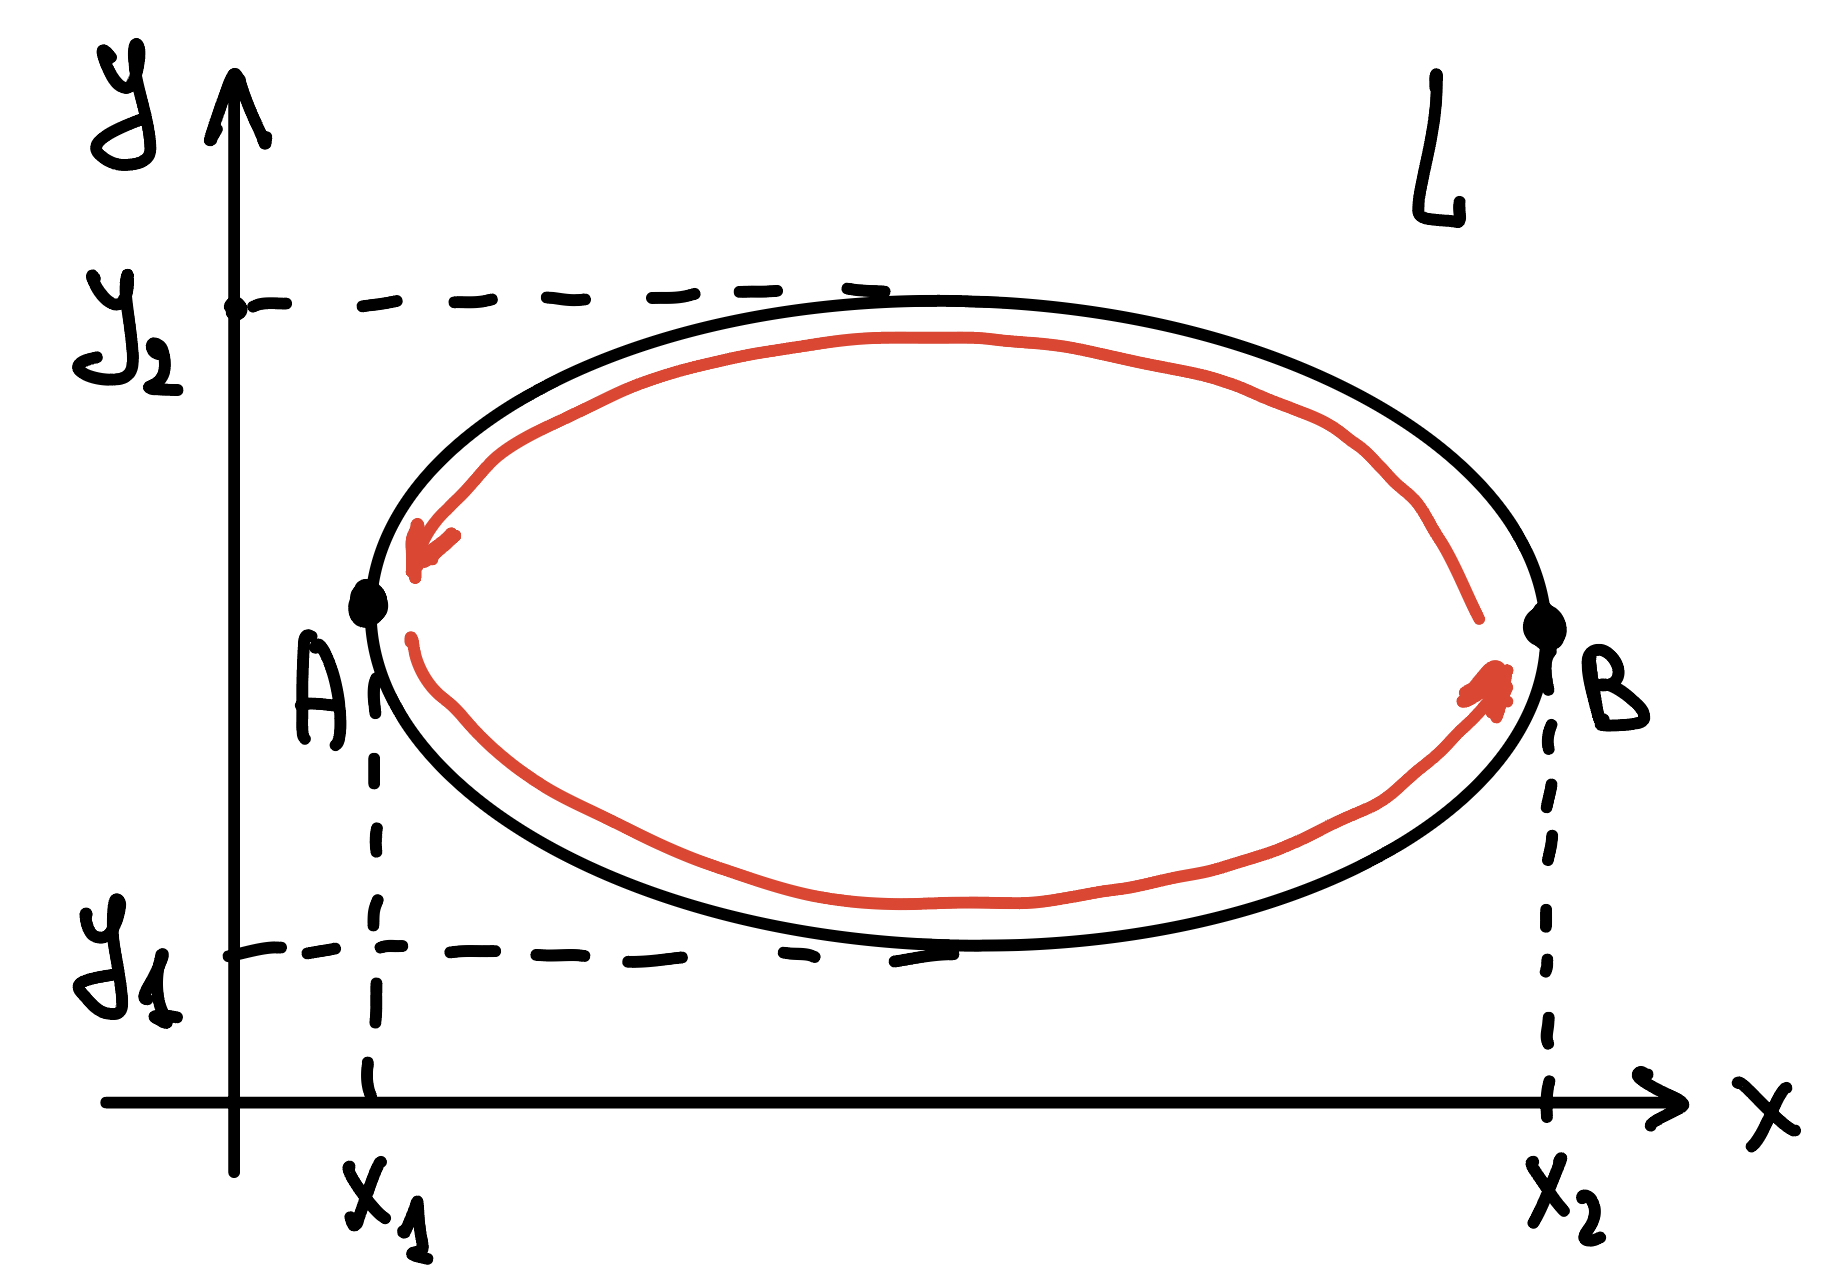
\includegraphics[scale=0.06]{pics/osn06_L.jpeg}

% Представим формулу Грина в покоординатной форме.

% \begin{proof}
% Введем ортонорм. Декартову сис. коорд.: $Oz \uparrow\uparrow \overline{k}$, $O_{xy}$ -- в плоскости $\pi$ и выбраны так, чтобы выполнялось "координатное свойство" на $D$
% $L: \{ x=x(t), ~ y = y(t) \}$ -- согласовано с направлением обхода.

% $\overline{a} = a_1(x,y,z)\overline{e}_1 + a_2(x,y,z)\overline{e}_2 + a_3(x,y,z)\overline{e}_3, ~ \overline{e}_3 = \overline{k}$, \\
% $rot(\overline{a}) = \dots + \left(\frac{\partial a_2}{\partial x} - \frac{\partial a_1}{\partial y} \right)\overline{e}_3 \Longrightarrow rot\left(\overline{a}, \overline{k}\right) = \frac{\partial a_2}{\partial x} - \frac{\partial a_1}{\partial y}$ в области $D$.

% $\overline{t} = \{x'(t), y'(t), 0\} \frac{1}{\sqrt{x'^2(t) + y'^2(t)}}$, $dl = \sqrt{x'^2(t) + y'^2(t)}dt \Longrightarrow
% \oint (\overline{a}, \overline{t})dl = \int_{t_1}^{t_2}(a_1(x,y,0)x'(t) + a_2(x,y,0)y'(t))dt = \oint\limits_{\mathcal{L}} (a_1(x,y,0)dx + a_2(x,y,0)dy)$

% $\iint\limits_{D}(\frac{\partial a_2}{\partial x} - \frac{\partial a_1}{\partial y})\bigg|_{z=0} dxdy$

% Пусть $P(x,y) = a_1(x,y,0), ~ Q(x, y) = a_2(x,y,0)$, тогда \textbf{Формула Грина} в покоординатной форме:
% $$\oint\limits_{L} (P(x,y)dx + Q(x,y)dy) = \iint\limits_{\overline{D}} (\frac{\partial Q}{\partial x} - \frac{\partial P}{\partial y}) dx dy$$
% \end{proof}

% Таким образом значение функции по третьей координате ($k$) не влияет на значение.
% Поэтому, не теряя общности, можем рассматривать функции, определенные только на плоскости: $a=\{P(x,y),Q(x,y)\}$.
% Докажем для этого прредставления для простой области.
% Пусть $L$ -- положительно ориентированная кусочно-гладкая замкнутая кривая на плоскости, а $D$ -- простая плоская область, ограниченная кривой $L$.
% Функции $P=P(x,y)$, $Q=Q(x,y)$ определены в области $D$ и имеют непрерывные частные производные $\frac{\partial P}{\partial y}, \frac{\partial Q}{\partial x}$.

% \begin{proof}
% Докажем по отдельности:

% \textbf{(1)}$ \oint\limits_{L}Pdx = \iint\limits_{\mathcal{D}}(-\frac{\partial P}{\partial y})dxdy$, 
% \textbf{(2)}$ \oint\limits_{L}Qdx = \iint\limits_{\mathcal{D}}(-\frac{\partial Q}{\partial y})dxdy$.

% $D: x_1 \leq x \leq x_2, ~ y_1(x) \leq y \leq y_2(x)$

% $(1) =\iint\limits_{\mathcal{D}}\frac{\partial P}{\partial y}dxdy = $
% $ -\int_{x_1}^{x_2}dx\int_{y_1(x)}^{y_2(x)} \left(\frac{\partial P}{\partial y} \right)dy = $
% $ -\int_{x_1}^{x_2}(P(x,y_2(x)) - P(x, y_1(x)))dx = -\int_{x_1}^{x_2}P(x, y_2(x))dx + \int_{x_1}^{x_2}P(x, y_1(x))dx = \int\limits_{\smile BA}P(x,y)dx + \int\limits_{\frown AB}P(x,y)dx$

% Аналогично, спроецируем D на $O_y$ - докажем вторую формулу.
% \end{proof}

\textbf{Формулировка}
Пусть $C$ -- положительно ориентированная кусочно-гладкая замкнутая кривая на плоскости, а $D$ -- область, ограниченная кривой $C$. 
Если 
%функция $P = P(x,y)$, $Q = Q(x,y)$ определены в области $D$ и имеют непрерывные частные производные
$\frac{\partial P}{\partial y}$, $\frac{\partial Q}{\partial x} \in \mathcal{C}(D)$, то

$\oint\limits_{C} P \,dx + Q \,dy = \iint\limits_{D} \left( \frac{\partial Q}{\partial x} - \frac{\partial P}{\partial y} \right) \,dx\,dy$

На символе интеграла часто рисуют окружность, чтобы подчеркнуть, что кривая $C$ замкнута.

\begin{proof}
\textbf{Доказательство ф. Грина для простой области}
%$D$ -- область, правильная в направлении $OY$, ограниченная замкнутой кривой $C$
\mathLet \ область $D$ -- криволинейная трапеция (область, правильная в направлении $OY$)
: $D = \{ (x,y)|a \le x \le b, y_1(x) \le y \le y_2(x) \}$

Для кривой $C$, ограничивающей область $D$ зададим направление обхода по часовой стрелке. Тогда:

$\iint\limits_{D} \frac{\partial P}{\partial y} \,dx\,dy = \int\limits_{a}^{b}dx \int\limits_{y_1(x)}^{y_2(x)} \frac{\partial P}{\partial y} \,dy = \int\limits_{a}^{b} (P(x,y_2(x)) - P(x,y_1(x))) \,dx =$
$= \int\limits_{a}^{b} P(x,y_2(x)) \,dx - \int\limits_{a}^{b} P(x,y_1(x)) \,dx \quad (1)$

Заметим, что оба полученных интеграла можно заменить криволинейными интегралами:
$\int\limits_{C_1} P(x,y) \,dx = -\int\limits_{-C_1} P(x,y) \,dx = -\int\limits_{a}^{b} P(x,y_1(x)) \,dx \quad (2)$
$\int\limits_{C_3} P(x,y) \,dx = \int\limits_{a}^{b} P(x,y_2(x)) \,dx \quad (3)$
Интеграл по $C_1$ берётся со знаком «минус», так как согласно ориентации контура $C$ направление обхода данной части -- от $b$ до $a$.

Криволинейные интегралы по $C_2$ и $C_4$ будут равны нулю, так как $x = \operatorname{const}$:
$\int\limits_{C_2} P(x,y) \,dx = 0 \quad (4)$
$\int\limits_{C_4} P(x,y) \,dx = 0 \quad (5)$

Заменим в (1) интегралы согласно (2) и (3), а также прибавим (4) и (5), равные нулю и поэтому не влияющие на значение выражения:\\
$\iint\limits_{D} \frac{\partial P}{\partial y} \,dx\,dy = \int\limits_{C_1} P(x,y) \,dx + \int\limits_{C_3} P(x,y) \,dx + \int\limits_{C_2} P(x,y) \,dx + \int\limits_{C_4} P(x,y) \,dx$

Так как обход по часовой стрелке при правой ориентации плоскости является отрицательным направлением, то сумма интегралов в правой части является криволинейным интегралом по замкнутой кривой $C$ в отрицательном направлении:
$\iint\limits_{D} \frac{\partial P}{\partial y} \,dx\,dy = -\int\limits_{C} P(x,y) \,dx \quad (6)$

Аналогично доказывается формула:\\
$\iint\limits_{D} \frac{\partial Q}{\partial x} \,dx\,dy = \int\limits_{C} Q(x,y) \,dy \quad (7)$
если в качестве области $D$ взять область, правильную в направлении $OX$.

Сложим (6) и (7):
$\int\limits_{C} P \,dx + Q \,dy = \iint\limits_{D} \left( \frac{\partial Q}{\partial x} - \frac{\partial P}{\partial y} \right) \,dx\,dy$
\end{proof}

% % -------- source --------
% \bigbreak
% [\cite[page 69-96]{replace_me}]
\vfill\null
\columnbreak
%---------------------2--------------------
\textbf{\LARGE osn 4. Числовые ряды. Абсолютная и условная сходимость. Признаки сходимости: Даламбера, интегральный, Лейбница.}

\textbf{Определения.}
\begin{itemize}
    \item Рассмотрим произвольную числовую последовательность $u_1,u_2,\dots,u_k,\dots$ и формально
    образуем из её элементов бесконечную сумму вида
    $u_1 +u_2 +\dots+u_k +\dots= \displaystyle \sum_{k=1}^{\infty}u_k$, называемую \textbf{числовым рядом}.
    Отдельные слагаемые $u_k$ называются \textbf{членами ряда}.
    Сумма первых $n$ членов ряда называется $n$-й \textbf{частичной суммой} ряда и обозначается $S_n$.
    Т.е. $S_n =u_1 +u_2 +\dots+u_n = \displaystyle \sum_{k=1}^n u_k$.
    \item Ряд называется \textbf{сходящимся}, если сходится последовательность $\{S_n\}$ частичных сумм этого ряда.
    При этом предел $S$ указанной последовательности $\{S_n\}$ называется \textbf{суммой ряда}.
    
    \item Ряд $\displaystyle \sum_{k=1}^{\infty}u_k$ называется \textbf{абсолютно сходящимся}, если ряд $\displaystyle \sum_{k=1}^{\infty}|u_k|$ также сходится.

    \item Ряд $\displaystyle \sum_{k=1}^{\infty}u_k$ называется \textbf{условно сходящимся}, если сам он сходится, а $\displaystyle \sum_{k=1}^{\infty}|u_k|$ расходится.
\end{itemize}

\textbf{Теоремы:}

\textbf{Критерий Коши} Ряд $\displaystyle \sum_{k=1}^n u_k$ сходится $\iff \forall \varepsilon > 0$ $\exists N$ $\forall n \geq N$ $ \forall p \in \mathbb{N} : \displaystyle \left|\sum_{k=n+1}^{n+p} u_k\right| < \varepsilon$.

\begin{proof}
    Обычный критерий Коши для последовательностей, с посл-ю частичных сумм: $|S_{n+p} - S_n| < \varepsilon$.
\end{proof}

Следствие: \textbf{Необходимое условие сходимости ряда:} $\lim_{k\rightarrow\infty} u_k=0$.

\begin{proof}
    Критерий Коши при $p = 1$.
\end{proof}

\bigbreak
\textbf{Признак Даламбера.}
Рассмотрим ряд $\displaystyle \sum_{k=1}^{\infty}p_k$,~$p_k > 0~\forall k \geqslant k_0 \geqslant 1$.

\textbf{П. I:} Если для всех номеров $k$, по крайней мере начиная с некоторого номера, справедливо неравенство
$\frac{p_{k+1}}{p_k} \leqslant q < 1 ~ \left( \frac{p_{k+1}}{p_k} \geqslant 1 \right)$,
то ряд $\displaystyle \sum_{k=1}^{\infty}p_k$ сходится (расходится).
    
\begin{proof}
Если $\frac{p_{k+1}}{p_k} \geqslant 1$, то $p_{k+1} \geqslant p_k$, а значит $\lim_{k\rightarrow\infty} u_k \neq 0$,
не выполнено необходимое условие сходимости ряда и ряд расходится.

Рассмотрим ряд из элементов геом. прогрессии: 

$\sum_{k=1}^{\infty} q^k = q + q^2 + \dots + \dots = \frac{1}{1-q}, \ |q| < 1$.

Если $\frac{p_{k+1}}{p_k} \leqslant q = \frac{q^{k+1}}{q^k}$, то ряд $\displaystyle \sum_{k=1}^{\infty}p_k$ сходится по признаку сравнения,
так как сходится ряд $\displaystyle \sum_{k=1}^{\infty}q_k$.
\end{proof}

\textbf{П. II:} Если $\exists$ предел $\displaystyle\lim_{k\rightarrow\infty}\frac{p_{k+1}}{p_k} = L$,
то ряд сходится при $L < 1$ и расходится при $L > 1$ (для $L=1$ признак не работает).


\begin{proof}
$\forall \varepsilon > 0$ $\exists N$ $\forall k \geq N : L - \varepsilon < \frac{p_{k+1}}{p_k} < L + \varepsilon$.
Выберем $\varepsilon = \frac{1}{2} |L-1|$.

Если $L < 1$, то $\frac{p_{k+1}}{p_k} < 0.5L + 0.5 = q < 1$, свели к 1 части, сходится.

Если $L > 1$, то $\frac{p_{k+1}}{p_k} > 0.5L + 0.5 > 1$, свели к 1 части, расходится.
\end{proof}

\bigbreak
\textbf{Интегральный признак Коши-Маклорена}.
Пусть при $x \geqslant 1$ функция $f(x) \geq 0$ и не возрастает.
Тогда ряд $\displaystyle \sum_{k=1}^{\infty}f(k)$ сходится или расходится одновременно с несобственным интегралом
$\int\limits_{1}^{\infty}f(x)dx$.

\begin{proof}
$\forall k \in \mathbb{N}$ $\forall x \in [k, k + 1]$, то $f(k) \geq f(x) \geq f(k+1) $
$\implies f(k) \geq \int_k^{k+1}f(x)dx \geq f(k+1), ~ k = 1, \dots, n-1, ~ (n \geq 2)$

$f(1) + f(2) + \dots + f(n-1) \geq \int\limits_1^n f(x)dx \geq f(2) + \dots + f(n)$

$S_n - p_1 \leq \int_1^n f(x)dx \leq S_{n-1}$

Если $\int_1^{+\infty} f(x)dx$ сходится, то $\int_1^n f(x)dx \leq M \implies S_n \leq M + p_1 \implies$ сходится 

Если $\int_1^{+\infty} f(x)dx$ расходится, то $\{f(x) \geq 0\} \int_1^n f(x)dx \rightarrow +\infty \implies S_{n-1} \rightarrow +\infty \implies$ расходится
\end{proof}

\bigbreak
\textbf{Признак Лейбница.}
Пусть последовательность $\{u_k\},~u_k>0~\forall k\in \mathbb{N}$ является невозрастающей и бесконечно малой.
Тогда знакочередующийся ряд $\displaystyle \sum_{k=1}^{\infty} (-1)^k u_k$ сходится.

\begin{proof}
$S_{2n} = (u_1 - u_2) + (u_3 - u_4) + \dots + (u_{2n-1} - u_{2n}) = (>0) + (>0) + \dots + (>0)$. Поэтому в силу
невозрастания последовательности $\{u_k\}$ последовательность $\{S_{2n}\}$ не убывает.
С другой стороны, ${S_{2n}} = u_1 - (u_2 - u_3) - \dots - (u_{2n-2} - u_{2n-1}) - u_{2n} = u_1 - (>0) - \dots - (>0) - u_{2n}$. Поэтому в силу
невозрастания последовательности $\{u_k\}$ и того, что $u_{2n} \geqslant 0$, последовательность
$\{S_{2n}\}$ ограничена сверху числом $u_1$. Следовательно, $\{S_{2n}\}$ сходится к некоторому
числу $S$. Но из того, что $S_{2n-1} = S_{2n} - u_{2n}$ и $\displaystyle \lim_{n\to \infty} u_{2n} = 0$ (из необх. условий сходимости), вытекает сходимость при $n\rightarrow\infty$
последовательности ${S_{2n-1}}$ к тому же $S$.
\end{proof}



% -------- source --------
\bigbreak
[\cite[page 7-22]{ilin_matan}]

\vfill\null
\columnbreak
%---------------------3--------------------
\textbf{\LARGE osn 2. Производная и дифференциал функций одной и нескольких переменных. Достаточные условия дифференцируемости.}

\textbf{Производной функции} $f(x)$ в точке $x_0$ называется предел при $\Delta x \to 0$ разностного отношения (если этот предел существует): $f'(x_0) = \lim \limits_{\Delta x \to 0}\frac{\Delta y}{\Delta x} = \lim \limits_{\Delta x \to 0} \frac{f(x_0+\Delta x)-f(x_0)}{\Delta x}$ ($x_0 + \Delta x \in$ области определения функции)

\bigbreak
Функция $f(x)$ называется \textbf{дифференцируемой в точке} $x_0$, если она определена в некоторой окрестности этой точки, а приращение $\Delta y$ этой функции в точке $x_0$, отвечающее приращению аргумента $\Delta x$, может быть представлено в виде $\Delta y = A \Delta x+ \omega(\Delta x)$, где $A$ --- не зависящее от $\Delta x$ конечное число, а $\omega(\Delta x) = o(\Delta x)$ при $\Delta x \to 0$

\bigbreak
Функция $u = f(x_1,\dots,x_m)$ называется \textbf{дифференцируемой в точке $M(x_1,\dots,x_m)$}, если её полное приращение в точке $M$ можно представить: 
$$ \Delta u= A_1 \Delta x_1 +\dots+A_m \Delta x_m + \alpha_1 \Delta x_1 +\dots+ \alpha_m \Delta x_m $$
где $A_1, \dots, A_m$ --- некоторые не зависящие от $\Delta x_1, \dots, \Delta x_m$ числа, а $ \alpha_1, \dots, \alpha_m$ --- бесконечно малые при $\Delta x_1 \to 0, \dots, \Delta x_m \to 0$ функции, равные 0 при $\Delta x_1 = \dots = \Delta x_m = 0$

\bigbreak
\textbf{Частная производная функции} $f(x_1,\dots,x_m)$ по переменной $x_i$ --- это предел отношения приращения функции по $x_i$ к приращению этой переменной, при стремлении этого приращения к нулю: $$ \frac{\partial f}{\partial x_i} = \lim\limits_{\Delta x \to 0}\frac{ f(x_1,\dots,x_i +\Delta x,\dots,x_m)-f(x_1,\dots,x_i,\dots,x_m)}{\Delta x}$$

\bigbreak
\textbf{Дифференциалом} $du$ дифференцируемой в $M(x_1,\dots,x_m)$ функции $u = f(x_1,\dots,x_m)$ называется главная линейная относительно приращений аргументов часть приращения этой функции в точке $M.$
$$du=A_1\Delta x_1 +\dots+A_m \Delta x_m = \frac{\partial u}{\partial x_1}\Delta x_1 +\dots+ \frac{\partial u}{\partial x_m}\Delta x_m$$

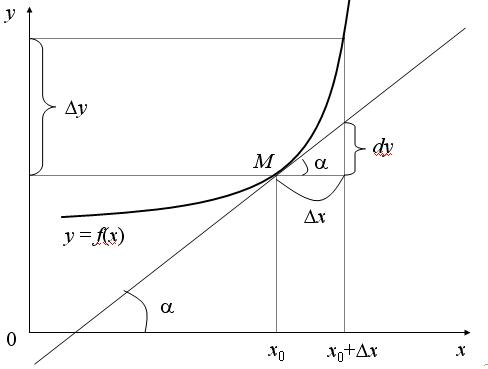
\includegraphics[scale=0.65]{pics/osn02_derivative.jpg}

\textbf{Критерий дифференцируемости для функции одной переменной}. Функция одной переменной $f(x)$ дифференцируема в точке $x_0$ $\iff$ она имеет в этой точке конечную производную.

\begin{proof} 
$(\implies) \Delta y = A \Delta x + \alpha(\Delta x)\Delta x \Rightarrow$ \{$\mathLet \Delta x \neq 0$\} $\Rightarrow \frac{\Delta y}{\Delta x}=A + \alpha(\Delta x) \Rightarrow \lim\limits_{\Delta x \to 0}\frac{\Delta y}{\Delta x}=A \Rightarrow f'(x) = A$\\
$(\impliedby) \mathLet \exists f'(x) < \infty. \mathLet \alpha(\Delta x)=\frac{\Delta y}{\Delta x}-f'(x)$, домножим на $\Delta x: \Delta y=f'(x)\Delta x+\alpha(\Delta x)\Delta x$
\end{proof}
\bigbreak

\textbf{Необходимое условие дифференцируемости для функций нескольких переменных.} Если $u = f(x_1,\dots,x_m)$ дифференцируема в $M(x_1,\dots,x_m)$, то в этой точке $\exists$ частные производные по всем аргументам, причём $\frac{\partial u}{\partial x_i} = A_i$, где $A_i$ определяются из условия дифференцируемости функции.

\begin{proof}
Из условия дифференцируемости вытекает, что частные приращения 
$\Delta u_i = A_i\Delta x_i+\alpha_i\Delta x_i$
$\Rightarrow \frac{\Delta u_i}{\Delta x_i} = A_i + \alpha_i $
$\Rightarrow \{\alpha_i \to 0$ при $\Delta x_i \to 0\} $
$\Rightarrow \lim\limits_{\Delta x_i \to 0}\frac{\Delta u_i}{\Delta x_i}=A_i$
\end{proof}

Условие не является достаточным, пример: $f(x, y) = \sqrt{\left|xy\right|}$ -- $\exists$ ч.п. 
$f'_x = \frac{1}{2} \sqrt{\frac{y}{x}}$, $f'_y = \frac{1}{2} \sqrt{\frac{x}{y}}$, но не дифф. в т. 0.
\bigbreak

\textbf{Достаточное условие дифференцируемости функций нескольких переменных.} Если $u = f(x_1,\dots,x_m)$ имеет частные производные по всем аргументам в некоторой окрестности точки $M_0(x^0_1, \dots, x^0_m)$, причём все эти частные производные непрерывны в точке $M_0$, то функция дифференцируема в точке $M_0$.

\begin{proof}
Для функции двух переменных $u=f(x,y)$: $\mathLet$ ч.п. $f'_x$ и $f'_y$ $ \exists$ в окр-ти точки $M_0(x_0,y_0)$ и непрерывны в этой точке, $\mathLet$ $M(x_0+\Delta x, y_0 + \Delta y)$ принадлежит указанной окрестности. \\
$\Delta u=f(x_0+\Delta x, y_0+\Delta y) - f(x_0, y_0) = [f(x_0+\Delta x, y_0+\Delta y)-f(x_0, y_0+\Delta y)] + [f(x_0, y_0+\Delta y) - f(x_0, y_0)]$ \\
$[f(x_0+\Delta x, y_0+\Delta y)-f(x_0, y_0+\Delta y)]$ -- приращение ф-ии одной переменной на сегменте $[x_0, x_0+\Delta x]$. Т.к. $u = f(x,y)$ имеет ч.п., то $f(x, y_0+\Delta y)$ дифф-ма и ее производная по $x = f'_x$. Применим к указанному приращению формулу Лагранжа: \\
$[f(x_0+\Delta x, y_0+\Delta y)-f(x_0, y_0+\Delta y)] = f'_x(x_0+\theta_1\Delta x, y_0+\Delta y)\Delta x, ~ \theta_1 \in (0,1)$.\\
Аналогично 
$[f(x_0, y_0+\Delta y)-f(x_0, y_0)] = f'_y(x_0, y_0+\theta_2\Delta y)\Delta y, ~ \theta_2 \in (0,1)$.

$f'_x$ и $f'_y$ непр. в т. $M_0 \Rightarrow f'_x(x_0+\theta_1\Delta x, y_0+\Delta y)=f'_x(x_0,y_0) + \alpha$, $f'_y(x_0, y_0+\theta_2\Delta y)\Delta y=f'_y(x_0,y_0) + \beta$, где $\alpha$ и $\beta$ -- беск. малые при $\Delta x \to 0, ~ \Delta y \to 0$ ф-ии. \\
Отсюда: $\Delta u=f'_x(x_0,y_0)\Delta x + f'_y(x_0,y_0)\Delta y + \alpha\Delta x + \beta\Delta y \Rightarrow u = f(x,y)$ -- дифф-ма в точке $M_0$.

Для ф-ии $m$ переменных $u=f(x_1, \dots, x_m)$ аналогично, представив $\Delta u$  в виде: \\
$\Delta u = f(x^0_1+\Delta x_1, \dots, x^0_m+\Delta x_m) - f(x^0_1, \dots, x^0_m) = \sum_{i=1}^{m}[f(x^0_1, \dots, x^0_i+\Delta x_i, \dots, x^0_m+\Delta x_m) - f(x^0_1, \dots, x^0_i, x^0_{i+1}+\Delta x_{i+1}, \dots, x^0_m+\Delta x_m)]$
\end{proof}




% -------- source --------

\vfill\null
\columnbreak
%---------------------
\end{multicols}
\end{tcolorbox}
% --- END OF PAGE ----



% --- BEGIN OF PAGE ----
\newpage
\begin{tcolorbox}[colback=white, left=0mm, right=0mm]
\begin{multicols}{4}
%---------------------0--------------------
\textbf{\LARGE osn 9. Ряд Фурье по ортогональной системе функций. Неравенство Бесселя, равенство Парсеваля,  сходимость ряда Фурье.}

Два элемента $f$ и $g$ евклидова пространства называются \textbf{ортогональными}, если скалярное произведение $\langle f, g \rangle = 0$.
Рассмотрим в произвольном бесконечномерном евклидовом пространстве $E$ некоторую последовательность элементов.
\begin{equation}
    \psi_1, \psi_2, \dots, \psi_n, \dots
    \label{asdfkjfnavw}
\end{equation}
Последовательность (\ref{asdfkjfnavw}) называется \textbf{ортонормированной системой}, если входящие в эту последовательность элементы попарно ортогональны и имеют норму, равную единице.

Пусть в произвольном бесконечномерном евклидовом пространстве $E$ задана произвольная ортонормированная система элементов $\{\psi_k\}$. Рассмотрим какой угодно элемент $f$ пространства $E$.

Назовём \textbf{рядом Фурье} элемента $f$ по ортонормированной системе $\{\psi_k\}$ ряд вида
$$\displaystyle\sum_{k=1}^{\infty} f_k\psi_k,$$
в котором через $f_k$ обозначены постоянные числа, называемые \textbf{коэффициентами Фурье} элемента $f$ и определяемые равенствами $f_k =\langle f,\psi_k\rangle, ~ k=1,2,\dots$

$S_n =\displaystyle\sum_{k=1}^{n}f_k\psi_k$ называется $n$-й \textbf{частичной суммой ряда Фурье}.

Рассмотрим наряду с $n$-й частичной суммой произвольную линейную комбинацию первых $n$ элементов ортонормированной системы $\{\psi_k\}$: $\displaystyle\sum_{k=1}^{n}C_k\psi_k$ с какими угодно постоянными числами $C_1, C_2, \dots, C_n$.

Величина $ \| f-g \|$ называется \textbf{отклонением} $f$ по норме данного евклидова пространства.

\textbf{Задача о начальном приближении:} $\displaystyle\min_{\forall\{C_j\}\in\mathbb{R}}  \|f-\displaystyle\sum_{k=1}^{n}C_k\psi_k \|$

Будем минимизировать квадрат нормы:

$ \| f-\displaystyle\sum_{k=1}^{n}C_k\psi_k \|^2 =  
\left\langle f-\displaystyle\sum_{k=1}^{n}C_k\psi_k, ~ f-\displaystyle\sum_{k=1}^{n}C_k\psi_k \right\rangle = 
\langle f, f \rangle - 2\displaystyle\sum_{k=1}^{n}C_k\langle f, \psi_k \rangle + \displaystyle\sum_{k=1}^{n} C_k^2 = 
\| f\|^2 + \displaystyle\sum_{k=1}^{n}(C_k^2-2C_kf_k) = 
\left\{ \pm \displaystyle\sum_{k=1}^{n}f_k^2 \right\} = 
\| f\|^2 - \displaystyle\sum_{k=1}^{n}f_k^2 + \displaystyle\sum_{k=1}^{n}(C_k-f_k)^2$,

минимум достигается при $ C_k = f_k,~k=1,2,\dots,n$. Таким образом, доказана следующая теорема:

\textbf{Теорема.} Среди всевозможных линейных комбинаций элементов ортонормированной системы $\{\psi_k\}$ евклидова пространства наименьшее отклонение от произвольного элемента  $f$ из пространства имеет $n$-я частичная сумма ряда Фурье элемента $f$ по системе $\{\psi_k\}$.

\textbf{Следствие 1.} $\forall$ элемента $f$ данного евклидова пространства, $\forall$ ортонормированной системы $\{\psi_k\}$ при произвольном выборе постоянных $C_k$ и $\forall n$ справедливо неравенство
$$ \| f \|^2-\displaystyle\sum_{k=1}^{n}f_k^2 \leqslant  \| \displaystyle\sum_{k=1}^{n}C_k\psi_k-f \|^2$$

\begin{proof}
$ \| f-\displaystyle\sum_{k=1}^{n}C_k\psi_k \|^2 = 
\| f\|^2 - \displaystyle\sum_{k=1}^{n}f_k^2 + \displaystyle\sum_{k=1}^{n}(C_k-f_k)^2 \geq \| f\|^2 - \displaystyle\sum_{k=1}^{n}f_k^2$
\end{proof}

\textbf{Следствие 2 (тождество Бесселя).} $\forall$ элемента $f$ данного евклидова пространства, $\forall$ ортонормированной системы $\{\psi_k\}$ и $\forall n$ справедливо равенство
$$ \| \displaystyle\sum_{k=1}^{n}f_k\psi_k-f \|^2 = \| f \|^2-\displaystyle\sum_{k=1}^{n}f_k^2$$

\begin{proof}
Подставить $C_k = f_k$ в $ \| f-\displaystyle\sum_{k=1}^{n}C_k\psi_k \|^2 = 
\| f\|^2 - \displaystyle\sum_{k=1}^{n}f_k^2 + \displaystyle\sum_{k=1}^{n}(C_k-f_k)^2$ 
\end{proof}

\textbf{Неравенство Бесселя.} $\forall$ элемента $f$ данного евклидова пространства, $\forall$ ортонормированной системы $\{\psi_k\}$ выполняется неравенство Бесселя: $$ \displaystyle\sum_{k=1}^{n}f_k^2 \leqslant \| f\|^2 $$

\begin{proof}
Из тождества Бесселя: $ \| \displaystyle\sum_{k=1}^{n}f_k\psi_k-f \|^2 \geq 0 \implies \| f \|^2-\displaystyle\sum_{k=1}^{n}f_k^2 \geq 0 \implies \| f \|^2 \geq \displaystyle\sum_{k=1}^{n}f_k^2$
\end{proof}

Ортонормированная система $\{\psi_k\}$ называется \textbf{замкнутой}, если $\forall$ элемента $f$ данного евклидова пространства $E$ и $\forall$ числа $\varepsilon > 0$ найдётся такая линейная комбинация конечного числа элементов $\{\psi_k\}$, отклонение которой от $f$ (по норме пространства $E$) меньше $\varepsilon$.

Другими словами, любой элемент пространства можно с любой степенью точности приблизить по норме этого пространства линейной комбинацией конечного числа первых элементов этой системы.

\textbf{Теорема.} Если ортонормированная система $\{\psi_k\}$ является замкнутой, то $\forall$ элемента $f$ рассматриваемого евклидова пространства неравенство Бесселя переходит в точное равенство
$$\displaystyle\sum_{k=1}^{\infty}f_k^2= \| f  \|^2,$$ называемое \textbf{равенством Парсеваля}.

\begin{proof}
Фиксируем произвольный элемент $f$ рассматриваемого евклидова пространства и произвольное $\varepsilon > 0$. 
Т.к система $f_k$ является замкнутой, то найдётся такой номер $n$ и такие числа $C_1, C_2, \dots, C_n$, что квадрат нормы, стоящий в правой части неравенства из следствия 1, будет меньше $\varepsilon$. В силу следствия 1 это означает, что для произвольного $\varepsilon > 0$ найдётся номер $n$, для которого
$ \| f  \|^2- \displaystyle\sum_{k=1}^{n}f_k^2 < \varepsilon$.

$\forall m > n$ это неравенство будет тем более справедливо, так как при возрастании номера $n$ сумма, стоящая в левой части может только возрасти.
В соединении с неравенством Бесселя это означает, что ряд  сходится к сумме $ \| f \|^2$.
\end{proof}

% -------- source --------

\vfill\null
\columnbreak
%---------------------1--------------------
\textbf{\LARGE osn 11. Алгебраические линии и поверхности второго порядка, канонические уравнения,  классификация.}

Если в пространстве $V_3$ зафиксированы точка $O$ и базис $\{e_1, e_2, e_3\}$, то говорят что в пространстве задана \textbf{афинная система координат} (или \textbf{общая декартова система координат}) $\{O, e_1, e_2, e_3\}$. Точка $O$ называется \textbf{началом координат}. Оси, проходящие через начало координат и определенные векторами $\{e_1, e_2, e_3\}$, называются \textbf{осями координат}. (Обозначается как $O_{xyz}$). Если вектора $e_i$ взаимно перепендикулярны, то задана \textbf{прямоугольная система координат}.

\bigbreak

Пусть $Oxy$ --- афинная система координат на плоскости. \textbf{Алгебраическая линия второго порядка} определяется уравнением $F(x, y) = 0$, где $F(x, y)$ --- алгебраический многочлен второй степени от переменных $x$ и $y$ с вещественными коэффициентами:
$$F(x,y)=a_{11}x^2 +2a_{12}xy+a_{22}y^2 +2a_{13}x+2a_{23}y+a_{33} =0,$$
$$~a_{11}^2 + a_{21}^2 + a_{22}^2\neq 0.$$
Это ур-е назывется \textbf{общим уравнением алгебраической линии второго порядка на плоскости}. Группа слагаемых $a_{11}x^2 + 2a_{12}xy + a_{22}y^2$ называется \textbf{квадратичной частью уравнения}, группа слагаемых $2a_{13}x + 2a_{23}y$ --- \textbf{линейной частью}, а $a_{33}$ --- свободным членом.

Введем обозначения:
$$A = \begin{pmatrix} a_{11} & a_{12} \\a_{12} & a_{22}\end{pmatrix},~ b=\begin{pmatrix} a_{13} \\ a_{23} \end{pmatrix},~ X=\begin{pmatrix}x \\ y\end{pmatrix},$$
$$B = \begin{pmatrix} a_{11} & a_{12} & a_{13} \\a_{12} & a_{22} & a_{23} \\ a_{13} & a_{23} & a_{33}\end{pmatrix} = \begin{pmatrix} A & b \\ b^T & a_{33}\end{pmatrix}$$

Тогда уравнение примет вид:
$$F(x,y) = X^TAX+2b^TX+a_{33}=0,~A=A^T,~A\neq\mathcal{O}.$$

\textbf{Теорема.} Общее уравнение линии второго порядка, заданное в прямоугольной декартовой системе координат, переходом к другой прямоугольной системе координат приводится к одному из следующих типов уравнений:
\begin{enumerate}
    \item $\lambda_1 x^2 + \lambda_2 y^2 + a_0 = 0$, где $\lambda_1\lambda_2\neq 0$
    \item $\lambda_2 y^2 + 2b_0x = 0$, где $\lambda_2 b_0\neq 0$
    \item $\lambda_2 y^2 + c_0 = 0$, где $\lambda_2\neq 0$
\end{enumerate}
Эти уранения называются \textbf{приведенными уравнениями} линии второго порядка.

\begin{proof}
\textbf{Шаг 1}: (преобразование базиса). \textbf{Метод вращений}. Если $a_{12} \neq 0$, то поворотом осей можно привести квадратичную часть $F(x,y)$ к сумме квадратов: $F(x,y) = a'_{11}x'^{2} + a'_{22}y'^{2} + a'_{13}x' + a'_{23}y' + a_{33} = 0$.

\textbf{Шаг 2}: (перенос начала). Если в полученном ур-е содержится ненулевой квадрат какой-либо переменной, то переносом начала можно освободиться от этой переменной в первой степени. Если $a'_{11} \neq 0$ и $a'_{22} \neq 0$, то 
$$
x'' = x' + \frac{a'_{13}}{a'_{11}}, \ y'' = y' + \frac{a'_{23}}{a'_{22}}, \ a'_{33} = a_{33} - \frac{{a'_{13}}^2}{a'_{11}} - \frac{{a'_{23}}^2}{a'_{22}}
$$

$$
a'_{11}x''^{2} + a'_{22}y''^{2} + a'_{33} = 0
$$
Все промежуточные и окончательные системы координат оставались прямоугольными, т.к. преобразования базиса с помощью ортогональной матрицы перехода сохраняют свойства ортонормированности.
\end{proof}


\textbf{Классификация ЛИНИЙ второго порядка}

\textbf{Теорема.} Общее уравнение линии второго порядка, заданное в прямоугольной декартовой системе координат, определяет одну и только одну из девяти линий. Для каждой из них существует прямоугольная система координат, в которой уравнение этой линии имеет \textbf{канонический вид}:

\textbf{I тип:}
\begin{enumerate}
    \item $\frac{x^2}{a^2} + \frac{y^2}{b^2} = \pm1$ --- эллипс (мнимый эллипс);
    \item $\frac{x^2}{a^2} \pm \frac{y^2}{b^2} = 0$ --- пара мнимых пересекающихся прямых (пара пересекающихся прямых); Только начало координат удовлетворяет ур-ю мним. пер. прям.
    \item $\frac{x^2}{a^2} - \frac{y^2}{b^2} = 1$ --- гипербола;
\end{enumerate}

\textbf{II тип:} $y^2 =2px,~p>0$ --- парабола;

\textbf{III тип:}
\begin{enumerate}
    \item $y^2 = \pm a^2,~a\neq 0$ --- пара параллельных прямых (пара мнимых параллельных прямых); Ни одна точна не удовлетворяет ур-ю мним. парал. прям.
    \item $y^2 = 0$ --- пара совпадающих прямых.
\end{enumerate}

\bigbreak

\textbf{Классификация ПОВЕРХНОСТЕЙ второго порядка}

Под \textbf{общим уравнением алгебраической поверхности} второго порядка в системе координат $Oxyz$ пространства понимают уравнение вида:

$F(x,y) = a_{11}x^2+a_{22}y^2+a_{33}z^2+2a_{12}xy+2a_{13}xz+2a_{23}yz+2b_1x+2b_2y+2b_3z+c=0$,
где не все коэффициенты $a_{ij}$ равны нулю, $a_{ij} = a_{ji}$

Введем обозначения:
$$A = \begin{pmatrix} a_{11} & a_{12} & a_{13} \\a_{12} & a_{22} & a_{23} \\ a_{13} & a_{23} & a_{33}\end{pmatrix},~ b=\begin{pmatrix} b_1 \\ b_2 \\ b_3 \end{pmatrix},~ X=\begin{pmatrix}x \\ y \\ z\end{pmatrix},
$$

$$~B = \begin{pmatrix} a_{11} & a_{12} & a_{13} & b_1 \\a_{12} & a_{22} & a_{23} & b_2 \\ a_{13} & a_{23} & a_{33} & b_3 \\ b_1 & b_2 & b_3 & c \end{pmatrix} = \begin{pmatrix} A & b \\ b^T & c\end{pmatrix}$$

Тогда уравнение примет вид:
$$F(x, y) = X^TAX+2b^TX+c=0,~A\neq\mathcal{O},~A=A^T.$$

\textbf{Теорема.} С помощью ортогонального преобразования координат (т.е. простым вращением и простым отражением) и параллельного перноса уравнение можно привести к одному из следующих типов:
\begin{enumerate}
    \item $\lambda_1x^2 + \lambda_2y^2 +\lambda_3z^2 + a_0 = 0, \ \lambda_1 \lambda_2 \lambda_3 \neq 0$
    \item $\lambda_1x^2 + \lambda_2y^2 + b_0z = 0, \ \lambda_1 \lambda_2 b_0 \neq 0$
    \item $\lambda_1x^2 + \lambda_2y^2 + c_0 = 0, \ \lambda_1 \lambda_2 \neq 0$
    \item $\lambda_2y^2 + p_0x = 0 , \ \lambda_1 p_o \neq 0$
    \item $\lambda_2y^2 + q = 0, \ \lambda_1 \neq 0$
\end{enumerate}


\textbf{Теорема.} Для любой алгебраической поверхности второго порядка существует прямоугольная декартова система координат, в которой уравнение этой поверхности имеет канонический вид:

\textbf{I тип:}
\begin{enumerate}
    \item $\frac{x^2}{a^2} + \frac{y^2}{b^2} + \frac{z^2}{c^2} = \pm1$ --- эллипсоид (мнимый эллипсоид); Ни одна точка пространства не удовлетворяет ур-ю мним. эллипс.
    \item $\frac{x^2}{a^2} + \frac{y^2}{b^2} + \frac{z^2}{c^2} = 0$ --- вырожденный эллипсоид; Удовлетворяет только начало координат.
    \item $\frac{x^2}{a^2} + \frac{y^2}{b^2} - \frac{z^2}{c^2} = \pm1$ --- однополостный гиперболоид (двухполостный гиперболоид);
    \item $\frac{x^2}{a^2} + \frac{y^2}{b^2} - \frac{z^2}{c^2} = 0$ --- конус;
\end{enumerate}

\textbf{II тип:}
 $ 2 Z = \frac{x^2}{a^2} \pm \frac{y^2}{b^2}$ --- эллиптический параболоид (гиперболический параболоид);

\textbf{III тип:}
\begin{enumerate}
    \item $\frac{x^2}{a^2} + \frac{y^2}{b^2} = \pm1$ --- эллиптический цилиндр (мнимый эллиптический цилиндр); Ни одна точка пространства не удовлетворяет ур-ю мним. эл. цил.
    \item $\frac{x^2}{a^2} - \frac{y^2}{b^2} = 1$ --- гиперболический цилиндр;
    \item $\frac{x^2}{a^2} + \frac{y^2}{b^2} = 0$ --- пара мнимых пересекающихся плоскостей;
    \item $\frac{x^2}{a^2} - \frac{y^2}{b^2} = 0$ --- пара пересекающихся плоскостей;
\end{enumerate}
\textbf{IV тип:} $y^2 = 2px,~p > 0$ --- параболический цилиндр;

\textbf{V тип:}
\begin{enumerate}
    \item $y^2 = \pm a^2$ --- пара параллельных плоскостей (пара мнимых параллельных плоскостей);
    \item $y^2 = 0$ --- пара совпадающих плоскостей.
\end{enumerate}


% -------- source --------
\bigbreak
[\cite[page 192-200, 329-341]{kim}]
\vfill\null
\columnbreak
%---------------------2--------------------
\textbf{\LARGE osn 13. Линейный оператор в конечномерном пространстве, его матрица. Норма линейного оператора.}


\textbf{Полем} называется множество $F$ с введенными на нем алгебраическими операциями сложения и умножения, а также если выполнены следующие аксиомы:
\begin{itemize}
    \item Коммутативность сложения: $\forall a,b \in F$ $a + b = b + a$
    \item Ассоциативность сложения: $\forall a,b,c \in F$ $(a + b) + c = a + (b + c)$
    \item Существование нулевого элемента: $\exists 0 \in F: \forall a \in F$ $a + 0 = 0$
    \item Существование противоположного элемента: $\forall a \in F \exists (-a) \in F: a + (-a) = 0$
    \item Коммутативность умножения: $\forall a, b \in F: a * b = b * a$
    \item Ассоциативность умножения: $\forall a,b,c \in F$ $(a * b) * c = a * (b * c)$
    \item Существование единичного элемента: $\exists e \in F\\ \{0\}: \forall a \in F$ $a * e = a$ 
    \item Существование обратного элемента для ненулевых элементов: $ (\forall a \in F: a \neq 0) \exists a^{-1} \in F: a * a^{-1} = e$
    \item Дистрибутивность умножения относительно сложения: $\forall a,b,c \in F$ $(a + b) *c = a * c + b * c$
\end{itemize}


\faEye \ множество $V$ элементов $x, y, z\dots$ и поле $P$ действительных или комплексных чисел. \mathLet \ в $V$ введены две операции: сложение его элементов и умножение его элементов на числа из $P$. 
Т.е $\forall x,y \in V$ определён элемент $z = x+y \in V$, а $\forall x \in V, ~ \forall \lambda \in P$ определён элемент $y = \lambda \cdot x \in  V$. \mathLet \ введённые две операции удовлетворяют \textbf{следующим аксиомам}:
\begin{enumerate}
    \item $x+y=y+x$;
    \item $(x+y)+z=x+(y+z)$;
    \item $\exists \theta\in V$, что $\forall x\in V \implies x+\theta=x$ ;
    \item $\forall x \in V ~ \exists (-x) \in V$, что $x + (-x) = \theta$;
    \item $1 \cdot x = x,~1 \in P$;
    \item $\lambda \cdot(x+y)=\lambda \cdot x+\lambda \cdot y,~\lambda \in P$;
    \item $(\lambda +\mu)\cdot x=\lambda \cdot x+\mu \cdot x,~\lambda,\mu \in P$;
    \item $(\lambda \mu )\cdot x = \lambda (\mu \cdot x)$.
\end{enumerate}
Тогда V называется \textbf{линейным пространством} над полем P.

Если P --- поле действительных чисел, то V --- \textbf{действительное линейное пространство}.

Если P --- поле комплексных чисел, то V --- \textbf{комплексное линейное пространство}.

Максимальное число линейно независимых векторов пространства V называется его \textbf{размерностью}. Если размерность пространства $V$ конечна, то оно называется \textbf{конечномерным}.

\mathLet \ даны 2 линейных пространства $V$ и W над общим полем $P$. Отображение $A :~V \to W$ называется \textbf{линейным отображением (линейным оператором)}, если для $\forall x, y \in V,~\alpha \in P$ выполнены равенства:
\begin{enumerate}
    \item $A(x + y) = A(x) + A(y)$;
    \item $A(\alpha x) = \alpha A(x)$;
\end{enumerate}

$\mathcal{L}(V, W)$ --- множество всех линейных операторов действующих из V в W.

\textbf{Простейшие свойства}.
\begin{enumerate}
    \item \textit{Линейный оператор переводит нулевой вектор в нулевой вектор}, так как $\mathcal{A}\theta_1 = \mathcal{A}(0x) = 0\mathcal{A}x = \theta_2$ (здесь $\theta_1,\theta_2$ - нулевые векторы пространств V и W соответственно)
    \item \textit{Линейный оператор сохраняет линейные комбинации}, т.е. переводит линейную комбиниацию векторов в линейную комбинацию образов с теми же коэффициентами: $\mathcal{A} \left( \sum_{i=1}^{k}\alpha_ix_i \right) = \sum_{i=1}^{k}\alpha_i\mathcal{A}x_i$
    \item \textit{Линейный оператор сохраняет линейную зависимость}, т.е. переводит линейно зависимую систему векторов в линейно зависимую.
\end{enumerate}

\textbf{Теорема.} $\mathLet ~ e_1, e_2,\dots,e_n$ --- базис пространства $V$, a $g_1,g_2,\dots,g_n$ --- любые векторы пространства $W$. Тогда существует единственный линейный оператор $A:~V \to W$, который переводит векторы $e_1, e_2,\dots,e_n$ в векторы $g_1,g_2,\dots,g_n$ соответственно.

\begin{proof} Строим оператор по правилу: если $x = \sum_{i=1}^{n} x_ie_i \in  V$, то $Ax = \sum_{i=1}^{n}x_iAe_i$. Из единственности разложения вектора по базису следует, что правило однозначно определяет образ $x$, при этом $Ae_i = g_i$. Линейность оператора вытекает из линейности координат. Если $B$ --- любой другой оператор, удовлетворяющий условию теоремы, то $Bx = \sum_{i=1}^{n} B(x_ie_i) = \sum_{i=1}^{n} x_ig_i = Ax \implies A$ единственен.
\end{proof}

\textbf{Матрица линейного оператора.}

$\mathLet ~ e_1, e_2,\dots,e_n$ и $f_1, f_2,\dots,f_m$ --- базисы конечномерных пространств $V$ и $W$. Линейный оператор $A:~V \to W$ однозначно определяется заданием векторов $Ae_1,\dots, Ae_n$. В свою очередь $Ae_i$ однозначно определяются своими координатами в базисе $f$:

$\begin{cases}
     Ae_1 = a_{11}f_1 + \dots + a_{m1}f_m&\\
     Ae_2 = a_{12}f_1 + \dots + a_{m2}f_m&\\
     \dots&\\
     Ae_n = a_{1n}f_1 + \dots + a_{mn}f_m&\\
\end{cases}$

$A_{fe} = \begin{pmatrix}a_{11} & \dots & a_{1n} \\ & \dots & \\ a_{m1} & \dots & a_{mn} \end{pmatrix}$ называется \textbf{матрицей оператора} $A$ в паре базисов $e$ и $f$.

$\mathLet ~ V$ --- линейное пространство над полем $P$.
\textbf{Нормой} в линейном пространстве V называется отображение $\|\cdot\|:~V \to R$, ставящее в соответствие каждому вектору $x \in V$ действительное число $\|x\| \in R$ и удовлетворяет аксиомам: $\forall x, y \in V, \alpha \in P$
\begin{enumerate}
    \item $\|x\| \geqslant 0$, причём норма равна нулю только если $x = 0$;
    \item $\|\alpha x\| = |\alpha| \cdot \|x\|$;
    \item $\|x + y\| \leqslant \|x\| + \|y\|$.
\end{enumerate}

Линейное пространство $V$ с заданной на нём нормой $\| \cdot \|$ называется \textbf{линейным нормированным пространством.} Число $\|x\|$ называется нормой вектора $x$.

$\mathLet ~ V, ~W$ --- линейные нормированные пространства с нормами $\| \cdot \|_V$ и $\| \cdot \|_W$. 
$\mathLet ~ \mathcal{L}(V, W)$ --- линейное пространство операторов, в котором можно ввести норму со следующими ограничениями $\forall \mathcal{A} \in \mathcal{L}(V, W)$:
\begin{itemize}
    \item \textbf{согласованность} с векторными нормами  $\| \cdot \|_V$ и $\| \cdot \|_W$: $\| \mathcal{A}x \|_W \leqslant \| \mathcal{A} \| \cdot \| x \|_V,~\forall x \in V$.
    \item \textbf{мультипликативность}: $\|\mathcal{A}\mathcal{B}\| \leqslant \| \mathcal{A}\|\cdot\|\mathcal{B}\|,~\forall\mathcal{A},\mathcal{B}$, для которых определено произведение $\mathcal{A}\mathcal{B}$.
\end{itemize}

\textbf{Теорема}. Собственное значение линейного оператора $\mathcal{A}\in\mathcal{L}(V,V)$ не превосходит по абсолютной величине любую его согласованную норму $\|\mathcal{A}\|$.

\begin{proof}
Если $\mathcal{A}x=\lambda x$, то для любой согласованной нормы оператора имеем $\| \mathcal{A}x \| = |\lambda| \cdot \| x \|$ и $\| \mathcal{A}x \| \leqslant \| \mathcal{A} \| \cdot \| x \|$, откуда следует, что $|\lambda| \leqslant \| \mathcal{A} \|$
\end{proof}

\textbf{Примеры операторных норм:}
\begin{itemize}
    \item $\mu(\mathcal{A}) = \displaystyle\sup_{\|x\|_V=1}\|\mathcal{A}x\|_W$ --- норма, \textbf{подчинённая} нормам $\| \cdot \|_V$ и $\| \cdot \|_W$, наименьшая из всех согласованных норм.
    \item $\|\mathcal{A}\|_2 = \displaystyle\sup_{\|x\|_V=1} \sqrt{(\mathcal{A}x,\mathcal{A}x)}$ --- \textbf{спектральная норма}, равная максимальному сингулярному числу (или максимальному по модулю собственному значению в случае нормального оператора).
    \item $\|\mathcal{A}\|_1 = \displaystyle\max_{1\leqslant j\leqslant n} \displaystyle\sum_{i=1}^{m}|a_{ij}|$ --- \textbf{максимальная столбцовая сумма}.
    \item $\|\mathcal{A}\|_{\infty} = \displaystyle\max_{1\leqslant i\leqslant m} \displaystyle\sum_{j=1}^{n}|a_{ij}|$ --- \textbf{максимальная строчная сумма}.
    \item $\|\mathcal{A}\|_E = \sqrt{\displaystyle\sum_{i,j}|a_{ij}|^2}$ --- \textbf{евклидова норма оператора.}
\end{itemize}




% -------- source --------
\bigbreak
[\cite[page 240-241, 352-353]{kim}]
\vfill\null
\columnbreak
%---------------------3--------------------
\textbf{\LARGE osn 15. Характеристический многочлен линейного оператора. Собственные числа и собственные векторы.}

\textbf{Линейным оператором} векторного пространства $V$ над полем $P$ в векторное пространство $W$ над тем же полем $P$ называется оператор $\mathcal{A} \in \mathcal{L}(V, W)$, удовлетворяющий условию линейности для всех $x, y \in V$ и $\alpha \in P$:
$$\mathcal{A} (x+y) = \mathcal{A} x + \mathcal{A} y$$
$$\mathcal{A} (\alpha x) = \alpha \mathcal{A} x$$

Пусть $e = (e_1, ..., e_n)$ и $f = (f_1, ..., f_m)$ -- базисы пространств $V$ и $W$. Линейный оператор $\mathcal{A} \in \mathcal{L}(V, W)$ однозначно определяется заданием векторов $\mathcal{A} e_1, ..., \mathcal{A} e_n$. В свою очередь вектора $\mathcal{A} e_i, i \in 1..n$ своими координатами в базисе $f$, т.е. коэффициентами разложений

$$\begin{cases} 
 \mathcal{A} e_1 = a_{11} f_1 + a_{21} f_2 + ... + a_{m1} f_m \\
 ... \\
 \mathcal{A} e_n = a_{1n} f_n + a_{2n} f_2 + ... + a_{mn} f_m
\end{cases}$$

Матрица $A_{fe} = 
\begin{bmatrix}
a_{11} & a_{12} & ... & a_{1n} \\
... & ... & ... & ... \\
a_{m1} & a_{m2} & ... & a_{mn} \\
\end{bmatrix}$
называется \textbf{матрицей линейного оператора} $\mathcal{A}$ в базисе $e$ и $f$. Матрицы линейного оператора в различных парах базисов эквивалентны.

Матрицы $A, B \in P^{m*n}$ называются \textbf{эквивалентными}, если существуют м-цы $D \in P^{m*m}, |D| \neq 0$ и $Q \in P^{n*n}, |Q| \neq 0$, такие что $B = D A Q$.

Квадратные матрицы $A, B \in P^{n*n}$ называются \textbf{подобными}, если существует м-ца $D \in P^{n*n}, |D| \neq 0$, такая что $B = D^{-1} A D$.

% ___думаю, это тут не нужно, в Киме есть теорема, но доказывать ее не хочется
% Подобные матрицы при задании одного и того же линейного оператора матрицей в разных координатных системах. При этом м-ца $D$ называется матрицей перехода от одной системы к другой.

\centerline{\textbf{Собственные числа и собственные векторы.}}

Пусть $V$ -- линейное пространство над полем $P$ и $\mathcal{A} \in \mathcal{L}(V, V)$.

Вектор $x: x\neq \theta, x \in V$ называется \textbf{собственным вектором} оператора $\mathcal{A}  = \mathcal{L}(V, V)$, если $\exists \lambda \in P$, такой что : 
$$\mathcal{A}x = \lambda x$$
$\lambda$ называется \textbf{собственным значением} оператора $\mathcal{A}$, соответствующим собственному вектору $x$.

\textbf{Спектр оператора} $\mathcal{A}$ -- это множество всех собственных значений $\mathcal{A}$.

\textbf{Теорема}: Собственные векторы, отвечающие различным собственным значениям, линейно независимы.

\begin{proof}
По индукции, для $n=1$ верно, т.к. с.в. $\neq \theta$ по определению. Пусть верно для из $n-1$ векторов, докажем для $n$.
От противного: пусть $x_1,\dots,x_n$ --- собственные векторы, отвечающие различным собственным значениям $\lambda_1,\dots,\lambda_n$, --- линейно зависимы. 
Тогда существует нетривиальная линейная комбинация этих векторов:
$$ \alpha_1x_1+\dots+\alpha_nx_n=\theta$$
Подействуем на неё оператором $A:~\alpha_1\lambda_1x_1+\dots+\alpha_n\lambda_nx_n=\theta$

Домножим линейную комбинацию на $\lambda_n:~\alpha_1\lambda_nx_1+\dots+\alpha_n\lambda_nx_n=\theta$

Вычтем первое равенство из второго, получим:
$$\alpha_1(\lambda_n-\lambda_1)x_1+\dots+\alpha_{n-1}(\lambda_n-\lambda_{n-1})x_{n-1}=\theta$$
Получили нетривиальную линейную комбинацию линейно независимых векторов, значит предположение неверно и теорема верна.
\end{proof}

\textbf{Следствие:} Линейный оператор, действующий в $n$-мерном пространстве, не может иметь более $n$ различных собственных значений.


\centerline{\textbf{Характеристический многочлен.}}

$f(\lambda) = |A - \lambda I|$ --- \textbf{характеристический многочлен} матрицы $A$.

Уравнение $det(\mathcal{A} - \lambda I) = 0$ --- \textbf{характеристическое уравнение} оператора $\mathcal{A}$.

\textbf{Теорема}: Характеристические многочлены подобных матриц совпадают, т.е.
    $A = Q^{-1}BQ \implies |A - \lambda I| = |B - \lambda I|$.

\begin{proof}
$|A - \lambda I| = |Q^{-1} B Q - \lambda I| = |Q^{-1} B Q - Q^{-1} \lambda I Q| = |Q^{-1} (B - \lambda I) Q| = |B - \lambda I|$. 

Т.е. $\forall \lambda$ характеристические многочлены м-ц $A$ и $B$ принимают одинаковые значения.
\end{proof}

\textbf{Следствие:} Все матрицы одного и того же линейного оператора имеют одинаковые характеристические многочлены.

\bigbreak

\textbf{Образом} лин. оператора $\mathcal{A} \in \mathcal{L}(V, W)$ наз-ся мн-во $im\mathcal{A} = \{y \in W | \exists x \in V : \mathcal{A}x=y \}$.

\textbf{Ядром} лин. оператора $\mathcal{A} \in \mathcal{L}(V, W)$ наз-ся мн-во $ker\mathcal{A} = \{x \in V | \mathcal{A}x=0 \}$.

\textbf{Теорема}: $\lambda$ --- собственное значение оператора $\mathcal{A} \iff \lambda$ --- корень характеристического уравнения оператора $\mathcal{A}$.

\begin{proof}
 $(\implies):~\lambda \in P$ --- собственное значение, $\exists x:~Ax = \lambda x,~x\neq 0,~(A - \lambda I)x = 0 \implies
    dim(ker(A - \lambda I))\neq 0 \implies det(A - \lambda I) = 0$.

    $(\impliedby):~\exists\lambda$ --- корень характеристического уравнения $\implies dim(im(A - \lambda I))
    \leqslant n - 1 \implies dim(ker(A - \lambda I)) \geqslant 1 \implies \exists x\neq\theta : (A - \lambda I)x = 0$.
\end{proof}



% -------- source --------
\bigbreak
[\cite[page 240-260]{kim}]
\vfill\null
\columnbreak
%---------------------
\end{multicols}
\end{tcolorbox}
% --- END OF PAGE ----


% --- BEGIN OF PAGE ----
\newpage
\begin{tcolorbox}[colback=white, left=0mm, right=0mm]
\begin{multicols}{4}
%---------------------0--------------------
\textbf{\LARGE osn 16.Формализация понятия алгоритма. Машины Тьюринга, нормальные алгоритмы Маркова. Алгоритмическая неразрешимость. Задача останова. Задача самоприменимости.}


\textbf{Интуитивное понятие алгоритма} --- четкая система действий, позволяющая определенным образом обработать входные данные и выдать результат решения задачи. Важен исполнитель алгоритма. Одна и та же система действий для одного исполнителя будет алгоритмом, а для другого --- нет.

Алгоритм \textbf{применим} к входным данным, если исполнитель за конечное число шагов остановится и выдаст (какой-то) ответ. В противном случае алгоритм \textbf{неприменим} к конкретным входным данным, т.е. он не остановится, либо завершит своё выполнение аварийно (сломается).

\textbf{Основные свойства алгоритма:}
\begin{enumerate}
    \item\textit{Определенность (понятность)}. Исполнитель алгоритма абсолютно точно знает, как выполнять все шаги алгоритма.
    \item \textit{Детерминированность}. Если алгоритм применим к конкретным входным данным, то он всегда и везде выдаст одинаковый ответ, а если неприменим, то всегда и везде зациклится или сломается.
    \item \textit{Дискретность или структурность.} Каждый достаточно сложный шаг алгоритма тоже является алгоритмом и может быть разложен на более простые шаги. Это же касается и обрабатываемых алгоритмом данных.
\end{enumerate}

Существуют разные способы формализации понятия алгоритма, \faEye \ два из них: машины Тьюринга и нормальные алгоритмы Маркова.


\textbf{Машина Тьюринга} --- гипотетическая машина (из-за использования бесконечной ленты). Автомат может двигаться вдоль ленты и по очереди обозревать содержимое ячеек. Он может находиться в одном из нескольких состояний $q_1,\dots, q_k$. В зависимости от того, какую букву $s_i$ автомат видит в состоянии $q_j$, то есть от пары $(s_i,q_j)$ (i --- номер ячейки, j --- номер состояния) автомат может выполнить следующие действия:
\begin{itemize}
    \item[--] запись новой буквы в обозреваемую ячейку; 
    \item[--] сдвиг влево или вправо на одну ячейку;
    \item[--] переход в новое состояние.
\end{itemize}


\textbf{Пример:} перенести первый символ непустого слова Р в его конец.
\begin{center}
\begin{tabular}{ |c||c|c|c|c||c| } 
\hline
       & a                   & b                   & c                  & $\Lambda$ & комментарий \\ 
\hline
\hline
 $q_1$ & $ \lambda, R, q_2 $ & $ \lambda, R, q_3 $ & $\lambda, R, q_4 $ & $, R,$    & анализ I симв., удаление \\ 
\hline
 $q_2$ & $, R,$              & $, R,$              & $, R,$             & $a, ,!$   & запись $a$ справа \\
\hline
 $q_3$ & $, R,$              & $, R,$              & $, R,$             & $b, ,!$   & запись $b$ справа \\
\hline
$q_4$  & $, R,$              & $, R,$              & $, R,$             & $c, ,!$   & запись $c$ справа \\
\hline
\end{tabular}
\end{center}

\textbf{Тезис Тьюринга:} если кто-то предложит какой-либо алгоритм обработки слов в заданном алфавите, то можно построить эквивалентную машину Тьюринга, которая будет применима и неприменима к одинаковым множествам слов.
В случае машины Тьюринга \textbf{алгоритм} --- это то, что может быть реализовано МТ.


\textbf{Нормальный алгоритм Маркова:}
        
Нет понятия ленты и подразумевается непосредственный доступ к любым частям преобразуемого слова. Пусть $A, B$ -- слова в некотором алфавите. Нормальный алгоритм можно записать в следующем виде: $A_i \left\{\begin{array}{lr} \to \\ \mapsto \end{array}\right\} B_i$.
Каждая пара -- формула подстановки для замены подслов в преобразуемом слове. Ищется вхождение слова $A_1$ в исходное слово. Если нашли, то заменяем его на $B_1$, если нет, то ищем $A_2$ и так далее. Затем возвращаемся в начало и снова ищем вхождение $A_1$. Процесс заканчивается, если ни одна из подстановок не применима, либо применилась завершающая формула, в которой $\mapsto$.

\textbf{Пример:} $A = \{a, b\}$. Преобразовать слово $P$ так, чтобы в его начале оказались все символы $a$, а в конце -- все символы $b$.

$$\begin{cases}
     ba \to ab &\\
\end{cases}$$

\textbf{Тезис Маркова:} если кто-то предложит какой-либо алгоритм обработки слов в заданном алфавите, то его можно нормализовать, т.е. построить эквивалентный нормальный алгоритм Маркова, который будет применим и неприменим к одинаковым множествам слов.
Машина Тьюринга и нормальные алгоритмы Маркова эквивалентны.

\centerline{\textbf{Самоприменимость}}

Входное слово, которое подаётся на вход алгоритму, может быть записью какого-то другого алгоритма. Когда алгоритм применим к своей записи, он называется \textbf{самоприменимым}.

\textbf{Теорема.} Если есть два алгоритма таких, что выходные данные одного можно использовать как входные данные для другого, то обязательно существует третий алгоритм, который работает как суперпозиция (композиция, последовательное выполнение) двух первых алгоритмов. [Давалась без док-ва]


\centerline{\textbf{Задача останова}} 

Пусть требуется построить алгоритм $X$, который, получая на входе запись любого алгоритма $A$ и его конкретные входные данные $D$, определяет, применим ли $A$ к этим данным $D$ (остановится ли $A$, получив на входе $D$).
    
\textbf{Теорема}. Такого алгоритма $X$ не существует. [Давалась без док-ва]
    
\centerline{\textbf{Алгоритмическая неразрешимость}}
Существуют задачи, для которых в принципе невозможно построить алгоритм их решения, они и называются \textbf{алгоритмически неразрешимыми}. Пусть требуется построить алгоритм $X$, который, получая на вход запись любого алгоритма $A$, определяет, самоприменим ли этот $A$, или нет. 
    
\textbf{Теорема.} Алгоритм $X$ не существует.

\begin{proof} Доказательство от противного. Пусть алгоритм $X$ существует, и, получив на вход запись алгоритма $A$, он вырабатывает ответ $DA$ (Да), если $A$ самоприменим, и ответ $NET$ (Нет), если несамоприменим.
Построим вспомогательный алгоритм $Y$ , вот его запись в форме НАМ:
$$\begin{cases} DA \to DA \\ NET \mapsto NET\end{cases}$$

Как видно, мы специально сделали так, чтобы выходные данные алгоритма $X$ можно подать на вход алгоритма $Y$. Тогда обязательно существует алгоритм $Z$, который работает как суперпозиция $X * Y$, то есть $Z = X * Y$. \faEye, самоприменим ли Z.
\begin{itemize}
    \item[--] Пусть $Z$ самоприменим, тогда $\langle \text{запись } Z\rangle Z \to \langle \text{запись } Z \rangle X * Y \to \langle DA \rangle Y \to $ Зациклились, предположение неверно.
    \item[--] Пусть Z несамоприменим, тогда $\langle \text{запись } Z \rangle Z \to \langle \text{запись } Z \rangle X * Y \to \langle NET \rangle Y \to $ Стоп, алгоритм самоприменим, предположение неверно.
\end{itemize} 
Как видно, оба предположения неверны, поэтому делаем вывод, что алгоритм $Z$ не существует. Однако алгоритм $Y$ существует (мы его построили), поэтому не существует алгоритм $X$. 
\end{proof}
    




% -------- source --------
\bigbreak
[\cite{pilschikov}]
\vfill\null
\columnbreak
%---------------------1--------------------
\textbf{\LARGE osn 14. Ортогональные преобразования евклидова пространства. Ортогональные матрицы и их свойства.}

Базисом линейного пространства называется упорядоченная линейно независимая система векторов пространства, через которую линейно выражается любой вектор пространства. 

Ортонормированным базисом называется
базис, векторы которого имеют единичную длину и в случае n>1 попарно перпендикулярны. 

\textbf{Ортогональные матрицы и их свойства.}
\begin{itemize}
    \item Матрица $Q \in \mathcal{C}^{n \times n}$ называется \textbf{унитарной}, если \newline $QQ^H = Q^HQ=I$
    \item Матрица $Q \in \mathcal{R}^{n \times n}$ называется \textbf{ортогональной}, если \newline $QQ^T = Q^TQ=I$
 
\end{itemize}   

$Q^H$ -- \textit{эрмитова-сопряженная матрица}: $q_{ji} = \overline{q}_{ij}$   \newline
$Q^T$ -- \textit{транспонированная матрица}: $q_{ij} = q_{ji}$

\textbf{Свойства ортогональной матрицы:}
    \begin{enumerate}
        \item $Q$ --- обратима, причём $Q^{-1}=Q^T$;
        
        \begin{proof}
        $\left|Q^T\right|=\left|Q\right| \implies \left|Q\right|^2 = 1 \implies \left|Q\right| \neq 0 \implies \exists Q^{-1}, Q^TQ=I \implies$ \{домн. справа на $Q^{-1}$ \} $\implies Q^T=Q^{-1}$
        \end{proof}
        
        \item $det(Q) = \pm1$;
        
        \begin{proof}
        $\left|Q^T\right|=\left|Q\right| \implies \left|Q\right|^2 = 1 \implies \left|Q\right| = \pm 1$
        \end{proof}
        
        \item $\forall \lambda$ --- собственное значение $Q\implies \lambda=\pm1$.
        \begin{proof}
        Пусть $Qx=\lambda x$ тогда $(x,x)=(x,Q^TQx) = (Qx,Qx) = (\lambda x,\lambda x) = \lambda^2(x,x) \Rightarrow (x,x) = \lambda^2(x,x) \Rightarrow \lambda^2 = 1$

        %$Qx=\lambda x, Q^Tx=\lambda x \implies Q^TQx=\lambda^2x=Ix \implies (\lambda^2 - 1) = \theta \implies %\lambda = \pm1$
        \end{proof}
    \end{enumerate}
 
Линейный оператор $\mathcal{U}$, действующий в унитарном (евклидомов) пространстве, называется \textbf{унитарным} (\textbf{ортогональным}) оператором, если $\mathcal{U}^*\mathcal{U} = \mathcal{U}\mathcal{U}^* = \mathcal{I}$
\begin{itemize}
\item Оператор $\mathcal{U}$ унитарен (ортогонален) $\iff$ в любом ортонормироавнном базисе он имеет унитарную (ортогональную) матрицу.
\item Для унитарного (ортогонального) оператора $\mathcal{U}$ справедливы равенства: \newline
$\mathcal{U}^* = \mathcal{U}^{-1}$, $|det\mathcal{U}| = 1$.
\item Унитарный (ортогональный) оператор нормален.
\end{itemize}

\textbf{Критерий унитарности}. В конечномерном унитарном (евклидовом) пространстве $\mathcal{V}$ следующие утверждения равносильны:
\begin{itemize}
\item Оператор $\mathcal{U}$ унитарен (ортогонален)
\item $\mathcal{U}^*\mathcal{U}$ = $\mathcal{I}$
\item $\mathcal{U}\mathcal{U}^*$ = $\mathcal{I}$
\item оператор $\mathcal{U}$ изометричен
\item оператор $\mathcal{U}$ сохраняет длину, т.е. $|\mathcal{U}x| = |x|, \forall x \in \mathcal{V}$
\item оператор $\mathcal{U}$ переводит любой ортонормированный базис $\mathcal{V}$ в ортонормированный базис
\item оператор $\mathcal{U}$ переводит хотя бы один ортонормированный базис $\mathcal{V}$ в ортонормированный базис
\end{itemize}

\begin{proof}
\begin{itemize}
\item $(1\Leftrightarrow 2)$ $(\implies)$ очевидно \\ $(\impliedby)$ $UU^*=I \implies \exists U^{-1}, UU^*=I$ \{домн. слева на $U^-1$\} $\implies U^*=U^{-1} \implies U^*U=I$ \\
\item $(1\Leftrightarrow 3)$ аналогично \\
\item $(3\Leftrightarrow 4)$ $(\implies)$ $(Ux, Uy)=(x,UU^*y)=(x,y)$ \\ $(\impliedby)$ $(Ux,Uy)=(x,y) \implies (x,UU^*y)=(x,Iy) \implies UU^*=I$ \\
\item $(4\Leftrightarrow 5)$ $(\implies)$ очевидно, т.к. $\left|x\right|=\sqrt{(x,x)}$ \\ $(\impliedby)$ a). $V$ -- евкл.: $(x,y)=(\left|x+y\right|^2-\left|x\right|^2-\left|y\right|^2)/2$ б). $V$ -- унит.: $(x,y)=(\left|x+y\right|^2-\left|x-y\right|^2+i\left|x+iy\right|^2-i\left|x-iy\right|^2)/2$ \\
\item $(4\Leftrightarrow 5)$ $(\implies)$ $e$ -- о/н $\implies (Ue_i,Ue_j)=(e_i,e_j)=\delta_{ij}$ \\ $(\impliedby)$ Пусть $e_1, \dots, e_n$ -- о/н. $\forall x \in V: x = \sum x_ie_i, Ux = \sum x_iUe_i \implies \left|x\right|^2 = \sum \left|x_i\right|^2, \left|Ux\right|^2 = \sum \left|x_i\right|^2 \implies U$ сохр. длину \\
\item $(6\Leftrightarrow 7)$ $(\implies)$ очевидно \\ $(\impliedby)$ доказано в предыдущем пункте $(\impliedby)$ \\
\end{itemize}
\end{proof}

\textbf{Примеры ортогональных матриц.}
\begin{itemize}
    \item $Q \in \mathbb{R}^{1\times1} \implies Q = \begin{bmatrix} \pm1\\ \end{bmatrix}$
    
    \item $Q \in \mathbb{R}^{2\times2} \implies 
    Q = \begin{bmatrix} 
        q_{11} & q_{12} \\
        q_{21} & q_{22} \\
    \end{bmatrix}$
    
    $QQ^T=Q^TQ=I \implies 
    \begin{cases}
    q_{11}^2 + q_{21}^2 = 1&\\
    q_{11}q_{12} + q_{21}q_{22} = 0&\\
    q_{12}^2 + q_{22}^2 = 1&\\
    \end{cases}
    \implies 
    \begin{cases}
    q_{11} = \cos\varphi&\\
    q_{21} = \sin\varphi&\\
    q_{12} = -kq_{21} = -k\sin\varphi&\\
    q_{22} = kq_{11} = k\cos\varphi&\\
    \end{cases}$
    
    \begin{enumerate}
        \item $k=1 \implies 
            Q = \begin{bmatrix} 
                \cos\varphi & -\sin\varphi \\
                \sin\varphi & \cos\varphi \\
            \end{bmatrix}$ (поворот).
            
        При $\varphi = \pi k$ получаются матрицы 
            $\begin{bmatrix} 
                1 & 0 \\
                0 & 1 \\
            \end{bmatrix}$, 
            $\begin{bmatrix} 
                -1 & 0 \\
                 0 & -1 \\
            \end{bmatrix}$.
            
        При $\varphi \ne \pi k$ матрица не диагонализируется, так как у неё нет вещественных собственных значений.
            
        \item $k=-1 \implies 
            Q = \begin{bmatrix} 
                \cos\varphi & \sin\varphi \\
                \sin\varphi & -\cos\varphi \\
            \end{bmatrix}$ (поворот и отражение).
        
        В этом случае собственные значения матрицы равны $\pm1 \implies$ 
        
        получаются матрицы 
        $\begin{bmatrix} 
            1 & 0 \\
            0 & -1 \\
        \end{bmatrix}$, 
        $\begin{bmatrix} 
            -1 & 0 \\
            0 & 1 \\
        \end{bmatrix}$.
    \end{enumerate}
    Таким образом, в случае $Q \in \mathbb{R}^{2\times2}$ для ортогонального оператора в евклидовом пространстве существует ортонормированный базис, в котором он имеет матрицу 
    
    либо 
    $\begin{bmatrix} 
        \pm1 & 0 \\
        0 & \pm1 \\
    \end{bmatrix}$, 
    
    либо 
    $\begin{bmatrix} 
        \cos\varphi & -\sin\varphi \\
        \sin\varphi & \cos\varphi \\
    \end{bmatrix},~(\varphi\ne\pi k)$.
\end{itemize}

\textbf{Теорема.} $\forall$ ортогонального оператора $Q$ в евклидовом пространстве $\exists$ ортонормированный базис $e$, в котором матрица оператора имеет вид:

$$ Q = \begin{bmatrix} 
            1 &    &   &   &   &   &   &   &   &   \\
              & \ddots  &  &   &   &   &   &   &   &   \\
              &  & 1  &    &   &   &   &   &   &   \\
              &   &   & -1 &   &   &   &   &   &   \\
              &   &   &  & \ddots &   &   &   &   \\
              &   &   &   &   & -1 &   &   &   &   \\
              &   &   &   &   &   & \cos\varphi_1 & -\sin\varphi_1 &  \\
              &   &   &   &   &   & \sin\varphi_1 & \cos\varphi_1 &  \\
              &   &   &   &   &   &   &   & \ddots\\
        \end{bmatrix} $$

\begin{proof} Доказательство методом математической индукции по размерности пространства $dim(V)=n$.

Для $n=1,~n=2$ теорема верна (выше рассмотрены все возможные случаи).

Пусть теорема верна для $n-1,~n-2$. Докажем для $n$. 

$Q$ действует в вещественном пространстве, а в нём существует либо одномерное, либо двумерное инвариантное подпространство $L$ ($\forall x \in L~Qx \in L$), для него можно найти базис. По свойствам ортогонального оператора $L^{\perp}$ (ортогональное подпространство) --- инвариантно относительно $Q$. $dim(L^{\perp})$ равна либо $n-1$, либо $n-2 \implies$ теорема для него верна. Совокупность базисов для $L$ и $L^{\perp}$ образует искомый базис с точностью до порядка базисных векторов.
\end{proof}


% -------- source --------
\bigbreak
[\cite[page 230-233, 292-295]{kim}]
\vfill\null
\columnbreak
%---------------------2--------------------
\textbf{\LARGE osn 12. Системы линейных алгебраических уравнений. Теорема Кронекера-Капелли. Общее решение системы линейных алгебраических уравнений.}

\textbf{Системой m линейных алгебраических уравнений с n неизвестными} называется совокупность отношений:
    $$\begin{cases}
        a_{11}x_1 + a_{12}x_2+\dots+a_{1n}x_n = b_1&\\
        a_{21}x_1 + a_{22}x_2+\dots+a_{2n}x_n = b_2&\\
        \dots&\\
        a_{m1}x_1 + a_{m2}x_2+\dots+a_{mn}x_n = b_m&\\
    \end{cases}$$
    
Упорядоченная совокупность чисел $c_1, ..., c_n \in\mathbb{R}$ называется \textbf{решением} системы, если при подстановке этих чисел в систему вместо неизвестных $x_1, ..., x_n$ соответственно каждое уравнение обращается в тождество.
Две СЛАУ \textbf{эквиваленты}, если множества их решений совпадают.
СЛАУ \textbf{совместна}, если существует хотя бы одно решение.
СЛАУ называется \textbf{определенной}, если она имеет единственное решение, если имеет больше одного -- \textbf{неопределенной}


\textbf{Теорема.} СЛАУ с квадратной невырожденной матрицей совместна и имеет единственное решение.

\begin{proof}
В силу невырожденности матрицы A для нее существует обратная матрица $A^{-1}$.
Вектор $x = A^{-1}b$ -- решение. Оно единственно. Если $y$ -- другое решение системы, то $Ax \equiv Ay$. Умножив обе части тождества слева на $A^{-1}$, получим $x = y$
\end{proof}

\textbf{Решение СЛАУ с помощью правила Крамера.}

Введём:
$A_i = \begin{pmatrix} a_{1,1} & \dots & a_{1,i-1} & b_1 & a_{1,i+1} & \dots & a_{1,n} \\
           a_{2,1} & \dots & a_{2,i-1} & b_2 & a_{2,i+1} & \dots & a_{2,n} \\
            & & & \dots & & & \\
           a_{n,1} & \dots & a_{n,i-1} & b_n & a_{n,i+1} & \dots & a_{n,n}
\end{pmatrix}$

Тогда: $x_i = \frac{|A_i|}{|A|},~i=1,\dots,n$. $A^{-1}$ получается из матрицы A заменой ее i-го столбца столбцом свободных членов.

$B = (A|b)$ --- \textbf{расширенная} матрица.
\newline
\textbf{Теорема Кронеккера-Капелли.} СЛАУ совместна $\iff$ $rgB = rgA$.

    \begin{proof}
    $(\implies)$ Пусть СЛАУ совместна $\implies \exists x_1, x_2, \dots, x_n:~a_1x_1 + a_2x_2 + \dots + a_nx_n = b \implies$ столбец $b$ является линейной комбинацией столбцов $a_1,\dots,a_n \implies rgB=rg(A|b) = rgA$
    
    $(\impliedby)$ Пусть $rgB = rg(A|b) = rgA = r$. Возьмём в матрице $A$ произвольный базисный минор. Так как $rg(A|b) = r$, то он же будет базисным минором матрицы $(A|b)$. Следовательно, последний столбец матрицы $(A|b)$ будет являться линейной комбинацией столбцов матрицы $A$. Коэффициенты этой комбинации являются решением СЛАУ $Ax=B$, то есть система совместна.
    \end{proof}

Пусть система
$$\begin{cases}
        a_{11}x_1+\dots + a_{1r}x_r+\dots+a_{1n}x_n = b_1&\\
        a_{21}x_1+\dots + a_{2r}x_r+\dots+a_{2n}x_n = b_2&\\
        \dots&\\
        a_{n1}x_1+\dots + a_{nr}x_r+\dots+a_{nn}x_n = b_n&\\
    \end{cases}$$

совместна и $rgA = rgB = r$. Будем считать, что базисный минор матрицы $A$ находится в левом верхнем углу:
$$M = \begin{vmatrix}
          a_{11} & \dots & a_{1r}\\
          & \dots & \\
          a_{r1} & \dots & a_{rr}
    \end{vmatrix} \neq 0 $$
Рассмотрим \textbf{укороченную} систему:
\begin{equation}
    \begin{cases}
        a_{11}x_1+\dots + a_{1r}x_r+\dots+a_{1n}x_n = b_1&\\
        a_{21}x_1+\dots + a_{2r}x_r+\dots+a_{2n}x_n = b_2&\\
        \dots&\\
        a_{r1}x_1+\dots + a_{rr}x_r+\dots+a_{rn}x_n = b_r&\\
    \end{cases}
    \label{eq1}
\end{equation}

\textbf{Теорема.} Укороченная система эквивалентна исходной системе.

\begin{proof}
Обе системы содержат одинаковое число неизвестных. Любое решение \textit{исходной} системы является рещением системы (\ref{eq1}). Покажем, что верно и обратное.
В расширенной матрице исходной системы первые $r$ строк являются базисными. Следовательно, все остальные строки согласно теореме о базисном миноре будут линейными комбинациями этих строк. Это означает, что каждое уравнение исходной системы, начиная с $(r+1)$-го, будет линейной комбинацией первых $r$ уравнений этой системы. Следовательно, каждое решение первых r уравнений исходной системы обращает в тождества все последующие уравнения.
\end{proof}

Запишем систему в виде
$$\begin{cases}
        a_{11}x_1+\dots + a_{1r}x_r = b_1-a_{1,r+1}x_{r+1} -\dots-a_{1n}x_n &\\
        a_{21}x_1+\dots + a_{2r}x_r= b_2-a_{2,r+1}x_{r+1} -\dots-a_{2n}x_n&\\
        \dots&\\
        a_{r1}x_1+\dots + a_{rr}x_r= b_r-a_{r,r+1}x_{r+1} -\dots-a_{rn}x_n&\\
    \end{cases}$$

Придав свободным членам $x_{r+1}, \dots, x_n$ произвольные значения $c_{r+1}, \dots, c_n$, получим систему уравнений относительно неизвестных $x_1, x_2, \dots, x_r$ с квадратной невырожденной матрицей:
\begin{equation}
    \begin{cases}
        a_{11}x_1+\dots + a_{1r}x_r = b_1-a_{1,r+1}c_{r+1} -\dots-a_{1n}c_n &\\
        a_{21}x_1+\dots + a_{2r}x_r= b_2-a_{2,r+1}c_{r+1} -\dots-a_{2n}c_n&\\
        \dots&\\
        a_{r1}x_1+\dots + a_{rr}x_r= b_r-a_{r,r+1}c_{r+1} -\dots-a_{rn}c_n&\\
    \end{cases}
    \label{eq2}
\end{equation}

Эта система имеет единственное решение $c_1, c_2, \dots, c_r$. Очевидно, совокупность $c_1, c_2, \dots, c_n$ является решением исходной системы.

\textbf{Теорема.} Придавая свободным неизвестным произвольные значения и вычисляя значения главных неизвестных, из полученной системы можно получить все решения исходной системы.

\begin{proof} Пусть $(c_1, \dots, c_r, c_{r+1}, \dots, c_n)$ --- произвольное решение (\ref{eq1}). Возьмём числа $(c_{r+1}, \dots, c_n)$ в качестве свободных переменных $x_{r+1}, \dots, x_n$ и будем вычислять значения главных неизвестных из системы (\ref{eq2}). Так как $(c_1, \dots, c_r, c_{r+1}, \dots, c_n)$ --- решение (\ref{eq1}), то $(c_1, \dots, c_r)$ --- решение системы (\ref{eq2}). Так как система (\ref{eq2}) имеет единственное решение, то в качестве решения можем получить только $(c_1, \dots, c_r)$. 
\end{proof}

\textbf{Опр.} Система линейных алгебраических уравнений с нулевой правой частью называется \textbf{однородной}.

\textbf{Теорема.} СЛАУ с $n$ неизвестными имеет единственное решение $\iff rgB = rgA = n$.

\begin{proof} Если $rgA < n$, то среди неизвестных будет хотя бы одно свободное неизвестное. Тогда получим бесконечно много решений. 
\end{proof}

\textbf{Общее решение СЛАУ}
Решим полученную систему (\ref{eq1}) относительно главных неизвестных: $x_1 = f_1(x_{r+1}, \dots, x_n), ~ \dots, ~ x_r = f_r(x_{r+1}, \dots, x_n)$, где $f_1, \dots, f_r$ -- однозначно определённые функции. Эти соотношения при произвольных $x_{r+1}, \dots, x_n$ описывают множество всех решений исходной системы и называются \textbf{общим решением} системы.
 
\todo{сюда бы пример нахождения общего решения}
 
\bigbreak
\begin{itemize}
    \item Однородная СЛАУ $Ax = 0$ всегда совместна: имеет тривиальное решение $x = \theta$.
    \item Однородная система с $n$ неизвестными имеет нетривиальное решение $\iff rgA < n$.
    \item Однородная система $Ax = 0$ с квадратной матрицей $A$ имеет нетривиальное решение $\iff |A| = 0$.
\end{itemize}






% -------- source --------
\bigbreak
[\cite[page 104-109]{kim}]
\vfill\null
\columnbreak
%---------------------3--------------------
\textbf{\LARGE osn 10. Прямая и плоскость, их уравнения. Взаимное расположение прямой и плоскости,  основные задачи на прямую и плоскость.}

Если в пространстве $V_3$ зафиксированы точка $O$ и базис $\{e_1, e_2, e_3\}$, то говорят что в пространстве задана \textbf{афинная система координат} (или \textbf{общая декартова система координат}) $\{O, e_1, e_2, e_3\}$. Точка $O$ называется \textbf{началом координат}. Оси, проходящие через начало координат и определенные векторами $\{e_1, e_2, e_3\}$, называются \textbf{осями координат}. (Обозначается как $O_{xyz}$)

Ненулевой вектор коллинеарный прямой называется ее \textbf{направляющим вектором}: $\overline{M_0M} = t \overline{a}$   

Два неколлинеарных вектора, параллельных плоскости, называются ее \textbf{направляющими векторами}. 


\bigbreak
\centerline{\textbf{Канонические уравнения.}}

\textbf{Уравнение прямой}. На плоскости в афинной системе координат $O_{xy}$ уравнение прямой \textit{l}, проходящей через точку $M_0(x_0,y_0)$ с направляющим вектором $\overline{a}=\{l,m\}$ имеет вид:
$$\begin{vmatrix} x-x_0 & y-y_0 \\ l & m \end{vmatrix} = 0 \iff \frac{x-x_0}{l} = \frac{y-y_0}{m} $$
\begin{proof}
$\mathLet M(x,y)$ -- точка. Тогда $\overline{M_0M}$ = $(x - x_0, ~ y - y_0)$. Условие $M_0M = ta$ в силу лин. координат означает, что в определении первая строка линейно выражена через вторую, а это равносильно определителю (выше). Равенство нулю определителя второго порядка равносильно пропорциональности его строк.
\end{proof}


\textbf{Уравнение плоскости}. 
В пространстве в афинной системе координат $O_{xyz}$ уравнение плоскости $\pi$, проходящей через точку $M_0(x_0,y_0,z_0)$ с направляющими векторами $\overline{p_i}=\{l_i,m_i,k_i\}$ $(i=1,2)$ имеет вид:
$$\begin{vmatrix} x-x_0 & y-y_0 & z-z_0\\ l_1 & m_1 & k_1 \\ l_2 & m_2 & k_2 \end{vmatrix} = 0 $$

\bigbreak
\centerline{\textbf{Параметрические уравнения.}}

\mathLet \ r = $\overline{OM}$, $r_0 = \overline{OM_0}$ -- радиус-векторы точек M и $M_0$ относительно полюса $O$. Если $\overline{a}$ - направляющий вектор, то $\overline{M_0M} = t\overline{a},~t\in\mathbb{R}$. Тогда $\overline{M_0M}$ = $r-r_0$ может быть записано в виде:

\textbf{Уравнение прямой}, проходящей через точку $M_0(\overline{r}_0)$ с направляющим вектором $\overline{a}=\{l,m\}$ имеет вид:
$$\overline{r} = \overline{r}_0 + \overline{a}t,~t\in\mathbb{R}$$

\textbf{Уравнение плоскости}, проходящей через точку $M_0(\overline{r}_0)$ с направляющими векторами $\overline{p}_i=\{l_i,m_i,k_i\}$, $(i=1,2)$ имеет вид:
$$\overline{r} = \overline{r}_0 + u\overline{p}_1 + v\overline{p}_2,~u,v\in\mathbb{R}$$

\bigbreak
\centerline{\textbf{Общие уравнения.}}

\textbf{Теорема}. Линия на плоскости (или поверхность в пространстве) --- есть прямая (плоскость) $\iff$ она является алгебраической линией (поверхностью) первого порядка, т. е. задается уравнением $$Ax+By+C=0,~A^2+B^2\neq0$$ $$(Ax+By+Cz+D=0,~A^2+B^2+C^2\neq0~\text{соответственно})$$ 
Это уравнение называется \textbf{общим уравнением} прямой на плоскости (плоскости в пространстве).

\begin{proof} $(\implies)$
$l$ --- прямая, каноническое уравнение прямой $\begin{vmatrix} x-x_0 & y-y_0 \\ l & m \end{vmatrix} = 0 \implies mx -ly -mx_0 +ly_0 = 0,~A=m,~B=-l,~C=-mx_0 +ly_0$, при этом $A^2+B^2\neq0$, так как $\overline{a}\neq 0$.

$(\impliedby)$ Рассмотрим линию $l:~Ax+By+C=0,~A^2+B^2\neq0$. Заметим, что при $x_0=-\frac{AC}{A^2+B^2},~y_0=-\frac{BC}{A^2+B^2}$ точка $M_0(x_0,y_0)\in l$. Вычитая из уравнения линии $Ax+By+C=0$ уравнение $Ax_0+By_0+C=0$, получим $A(x-x_0)+B(y-y_0)=0$, а значит $\begin{vmatrix} x-x_0 & y-y_0 \\ -B & A \end{vmatrix} = 0$ --- каноническое уравнение прямой, проходящей через точку $M_0$, с направляющим вектором $\{-B,A\}$, а значит линия $l$ --- прямая. 
\end{proof}
    


\textbf{Взаимное расположение прямой и плоскости.} 

\mathLet \ плоскость $\pi$ задана общим уравнением $Ax + By + Cz + D = 0$, а прямая $l$ задана каноническим уравнением $\frac{x-x_0}{m} = \frac{y-y_0}{n} = \frac{z-z_0}{k}$, $M(x_0, y_0, z_0) \in l$, $\overline{p} = (A, B, C)$ -- вектор нормали. Тогда:
\begin{enumerate}
    \item Прямая $l$ принадлежит плоскости $\pi$ $\iff$ \newline
    $
    \begin{cases}
        M \in \pi \implies Ax_0 +By_0 +Cz_0 +D = 0 \\
        (l, \overline{p}) = 0  \implies Am+Bn+Ck = 0
    \end{cases}
    $
    \item Прямая $l$ параллельна плоскости $\pi$ $\iff$ \newline
    
    $\begin{cases}
        M \notin \pi \implies Ax_0+By_0+Cz_0+D\neq 0 \\
        (l, \overline{p}) = 0  \implies Am+Bn+Ck = 0
    \end{cases}$
    
    \item Прямая $l$ перпендикулярна плоскости $\pi$ $\iff$ \newline
    $l \| \overline{p} \implies$ $\frac{A}{m} = \frac{B}{n} = \frac{C}{k}$.
    
    \item Угол $\varphi$ между прямой $l$ и плоскостью $\pi$: \newline
    $$  sin\varphi = sin(l, \pi) = \frac{| (l, \overline{p}) |}{|l| \cdot |\overline{p}|} = \frac{|Am+Bn+Ck|}{\sqrt{A^2+B^2+C^2}\cdot\sqrt{m^2+n^2+k^2}}$$
\end{enumerate}
   
\textbf{Основные задачи на прямую и плоскость.}

\textbf{Углом между двумя прямыми в пространстве} называется любой из углов между параллельными им прямыми, проходящими через какую-либо точку пространства. Таким образом, две прямые в пространстве образуют между собой два различных угла в сумме равных $\pi$. Угол между направляющими вектоами прямых равен одному из этих углов. Угол между прямыми $l_i: r = r_i + ta_i, i = 1,2$, совпадающий с угом между направляющими векторами $a_i = \{m_i, n_i, k_i\}$:

$$cos\varphi = \frac{m_1m_2 + n_1n_2 + k_1k_2}{\sqrt{m_1^2 + n_1^2 + k_1^2}\sqrt{m_2^2 + n_2^2 + k_2^2}}$$

\textbf{Углом между прямой и плоскостью} (если они не перпендикулярны) называется меньший из углов между этой прямой и ее ортогональной проекцией на плоскость. 
Если же прямая и плоскость перпендикулярны, то угол между ними считается равным $\pi / 2$. 
Угол $\varphi$ между прямой $l: r = r_0 + ta$ и плоскостью $\pi: Ax + By + Cz + D = 0$ находится как
дополнительный к углу между направляющим вектором прямой $\overline{a} = \{m, n, k\}$ 
и вектором нормали к плоскости $\overline{n} = \{A, B, C\}$ и вычисляется:

$$sin\varphi = \frac{|Am + Bn + Ck|}{\sqrt{m^2 + n^2 + k^2}\sqrt{A^2 + B^2 + C^2}}, ~ 0 \leq \varphi \leq \pi / 2$$

\textbf{Расстояние $\rho(M_1, l)$ от точки $M_1(r_1)$} до прямой $l: r = r_0 + ta$ находится как высота h параллелограмма, построенного на векторах a и $\overline{M_0M_1}$ площадь и основание которого известны

$$\rho(M_1, l) = \frac{|[a, r_1 - r_0]|}{|a|}$$

\textbf{Расстоянием между скрещивающимися прямыми} $l_i: r = r_i + ta_i, ~ i = 1,2$ называется расстояние между параллельными плоскостями, в которых лежат прямые $l_1, l_2$. Это расстояние $\rho(l_1, l_2)$ находится как высота параллелепипеда, построенного на векторах $\overline{M_1M_2}, a_1, a_2$, объем и площадь основания которого известны:

$$\rho(l_1, l_2) = \frac{|(r_2 - r_1, a_1, a_2)|}{|[a_1, a_2]|}$$

\textbf{Найти уравнение прямой $l$:} $l$  проходит через т. $M_0(x_0,y_0,z_0)$ и перпендикулярна плоскости $Ax+By+Cz+D=0$. Ответ: $\frac{x-x_0}{A} = \frac{y-y_0}{B} = \frac{z-z_0}{C}$.

\textbf{Найти уравнение плоскости $\pi$:} $\pi$ проходит через т. $M_0(x_0,y_0,z_0)$ и перпендикулярна прямой $\frac{x-x_1}{m} = \frac{y-y_1}{n} = \frac{z-z_1}{k}$. Ответ: $m(x-x_0)+n(y-y_0)+k(z-z_0) = 0$.

\textbf{Найти уравнение плоскости $\pi$:} $\pi$ проходит через прямую $\frac{x-x_1}{m} = \frac{y-y_1}{n} = \frac{z-z_1}{k}$ и через т. $M_0(x_0,y_0,z_0)$, не лежащую на этой прямой. Ответ: $$\begin{vmatrix} x-x_0 & y-y_0 & z-z_0\\ x_1-x_0 & y_1-y_0 & z_1-z_0 \\ m & n & k \end{vmatrix} = 0 $$

\textbf{Найти уравнение плоскости $\pi$:} $\pi$ проходит через прямую $\frac{x-x_1}{m_1} = \frac{y-y_1}{n_1} = \frac{z-z_1}{k_1}$ и параллельна другой данной прямой $\frac{x-x_2}{m_2} = \frac{y-y_2}{n_2} = \frac{z-z_2}{k_2}$ (две данные прямые не параллельны). Ответ: $$\begin{vmatrix} x-x_1 & y-y_1 & z-z_1\\ m_1 & n_1 & k_1 \\ m_2 & n_2 & k_2 \end{vmatrix} = 0 $$

\textbf{Найти уравнение плоскости $\pi$:} $\pi$ проходит через две данные точки $M_0(x_0,y_0,z_0)$ и $M_1(x_1,y_1,z_1)$ и  перпендикулярна данной плоскости $Ax + By + Cz + D = 0$ (прямая $M_0M_1$ и данная плоскость не перпендикулярны). Ответ: $$\begin{vmatrix} x-x_0 & y-y_0 & z-z_0\\ x_1-x_0 & y_1-y_0 & z_1-z_0 \\ A & B & C \end{vmatrix} = 0 $$
\vfill\null
\columnbreak
%---------------------
\end{multicols}
\end{tcolorbox}
% --- END OF PAGE ----



% --- BEGIN OF PAGE ----
\newpage
\begin{tcolorbox}[colback=white, left=0mm, right=0mm]
\begin{multicols}{4}
%---------------------0--------------------
\textbf{\LARGE osn 17. Понятие архитектуры ЭВМ. Принципы фон Неймана. Компоненты компьютера: процессор, оперативная память, внешние устройства. Аппарат прерываний.}


\textbf{Компьютер} --- исполнитель алгоритма на языке машины.

\textbf{Архитектура ЭВМ} --- совокупность узлов машины и взаимосвязей между ними, рассматриваемая на определённом уровне рассмотрения этой архитектуры.

\textbf{Принципы фон Неймана:}
\begin{enumerate}
    \item Принцип двоичного кодирования информации: вся информация, которая поступает и обрабатывается в компьютере, кодируется в двоичной системе счисления.
    \item Принцип программного управления. Программа состоит из команд, в которых закодированы операция и операнды, над которыми должна выполниться данная операция. Выполнение компьютером программы — это автоматическое выполнение определенной последовательности команд, составляющих программу. В компьютере устройство, обеспечивающее выполнение команд, — Последовательность выполняемых процессором команд последовательностью команд и данных, составляющих программу. То есть, по сути, второй принцип – это принцип последовательной обработки.
    \item Принцип хранимой программы. Для хранения команд и данных программы используется единое устройство памяти, которое представляется в виде вектора слов. Все слова имеют последовательную адресацию. Команды и данные представляются единым образом. Интерпретация информации памяти и, соответственно, ее идентификация как команды или как данных происходит неявно при выполнении очередной команды. К примеру, содержимое слова, адрес которого используется в команде перехода в качестве операнда, интерпретируется как команда. Если то же слово используется в качестве операнда команды сложения, то его содержимое интерпретируется как данные. То есть одна и та же область памяти в зависимости от команд в одном случае будет интерпретироваться как команда, в другом случае – как данные. Этот принцип фон Неймана замечателен тем, что он определяет возможность программной генерации команд с последующим их выполнением, то есть возможность компиляции программы, когда одна программа порождает другую программу, которая будет выполняться.
\end{enumerate}

\textbf{Процессор} состоит из \textit{устройства управления (УУ)} и \textit{арифметико-логического устройства (АЛУ)}. АЛУ выполняет различные операции над данными, хранящимися на регистрах АЛУ. УУ выполняет команды языка машины, посылая управляющие сигналы к остальным устройствам.

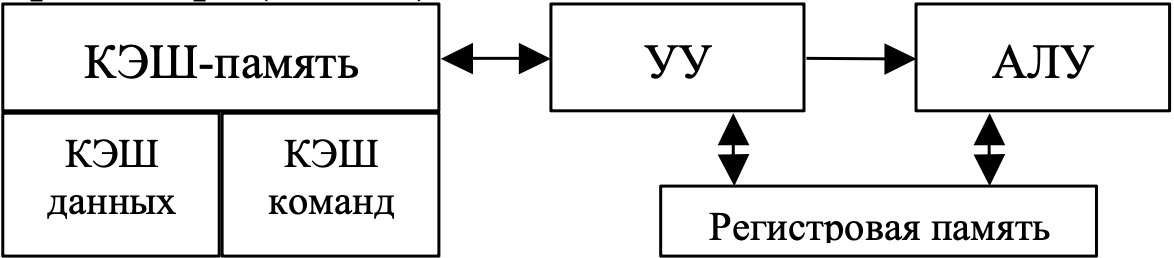
\includegraphics[width=\columnwidth]{pics/CPU.png}

\textbf{Основная (оперативная) память} хранит команды программы и обрабатываемые данные. ОЗУ состоит из ячеек, ячейка памяти - устройство, в котором размещается информация. Ячейка состоит из двух полей \textit{тег} и \textit{машинное слово}. Машинное слово - поле программно изменяемой информации. Здесь могут располагаться машинные команды или данные, с которыми будет оперировать программа. Имеет фиксированный для данной ЭВМ размер. Размер машинного слова - количество двоичных разрядов, размещаемых в машинном слове. Поле машинной информации (тег) - поле ячейки памяти, в котором схемами контроля процессами и ОЗУ автоматически размещается информация, необходимая для осуществления контроля за целостностью и корректностью использования данных. Использование тега:
\begin{itemize}
    \item Контроль за целостностью данных - одноразрядный тег, который использовался для контроля точности.
    \item Контроль доступа к командам/данным. (вся информация раскрашивается в 2 цвета - команды и данные)
    \item Контроль доступа к машинным типам данных. (в теге записывается код типа данных)
\end{itemize}

Ячейки памяти, расположенные не в основной памяти ЭВМ, а в других устройствах, называются регистрами. В процессе работы команды поступают на регистры в УУ, а данные --- на регистры в АЛУ. АЛУ может обрабатывать данные только на своих регистрах, чтобы обработать данные, расположенные в основной памяти, их надо сначала считать на регистры в АЛУ.

\textbf{Внешние устройства} служат для обмена программами и данными между основной (оперативной) памятью и <<внешним миром>>.


\centerline{\textbf{Аппарат прерываний}}

\textbf{Аппарат прерываний} -- способность ЭВМ быстро и гибко реагировать на события, происходящие как внутри процессора и оперативной памяти, так и во внешних устройствах. Каждое такое событие порождает сигнал, приходящий на специальную электронную схему -- контроллер прерываний.

Прерывания делятся на:
\begin{itemize}
    \item[--] \textit{Внутренние (синхронные)}, источником которых являются выполняемые команды программы, их нельзя закрыть и не реагировать на них.
    \item[--] \textit{Внешние (асинхронные)}, которые вызываются событиями в периферийных устройствах. Эти прерывания можно временно закрыть, если в данный момент процессор занят другой срочной работой.
\end{itemize}
    
\textbf{Аппаратная реакция} на прерывание заключается в сохранении информации о считающейся в данное время программе (процесса) и переключение на выполнение другой программы (процедуры обработки прерывания, т.е. события, здесь включается режим блокировки прерываний). В некоторых архитектурах это называется переключением контекста. Этот механизм позволяет (при необходимости) продолжить (возобновить) выполнение прерванной программы с текущего места.

\textbf{Программная реакция} на прерывание производится процедурой-обработчиком прерывания и делится на два этапа. Сначала происходит минимальная программная реакция, она производится в режиме с закрытыми прерываниями от внешних устройств. Это опасный режим, так как процессор не обращает внимание на все события в периферийных устройствах. Затем происходит полная программная реакция уже в режиме с открытыми прерываниями.

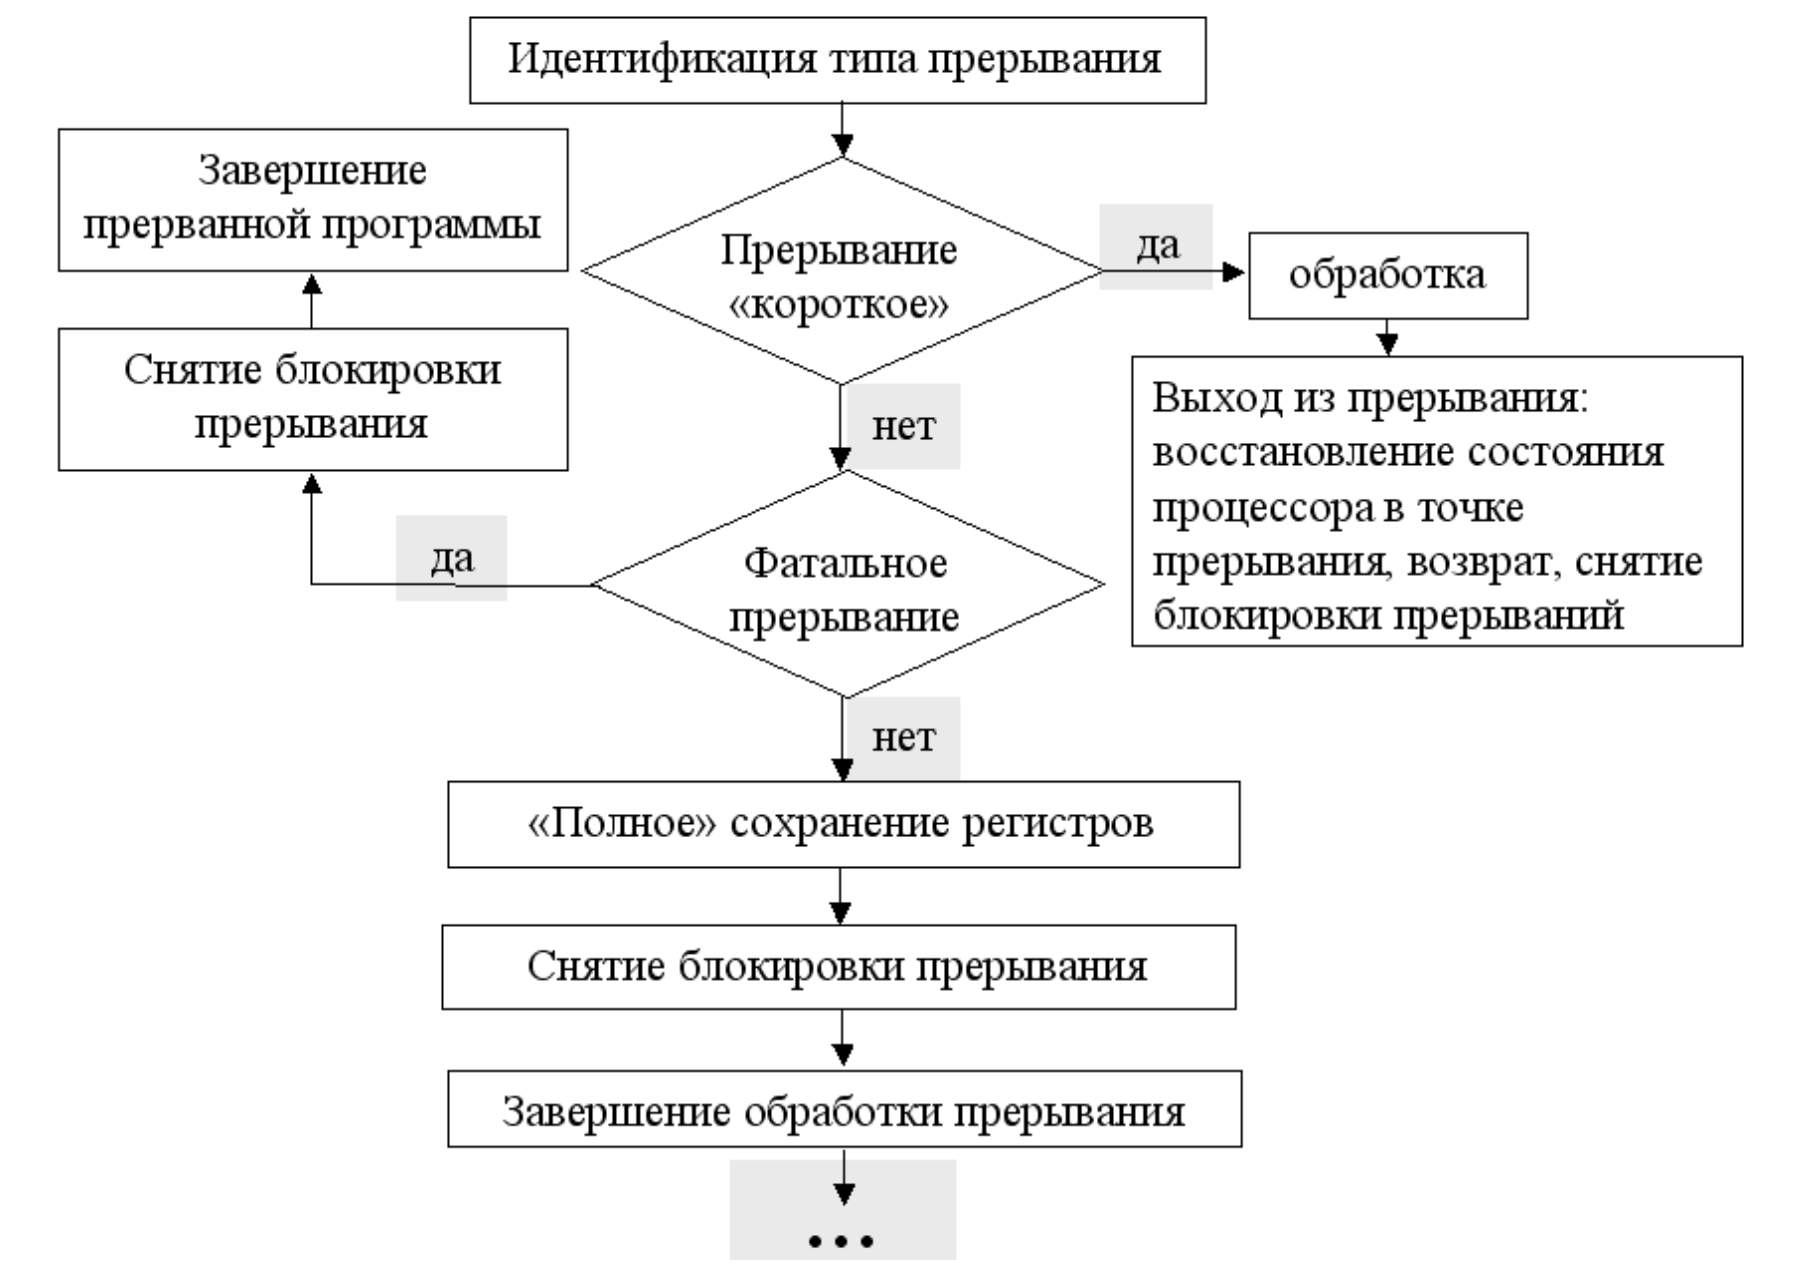
\includegraphics[scale=0.31]{pics/interruptions.png}

\textbf{Короткое прерывание} -- обработка не требует дополнительных ресурсов ЦП и времени.

\textbf{Фатальное прерывание} -- после него продолжить выполнение программы невозможно.


% % -------- source --------
% \bigbreak
% [\cite[page 69-96]{replace_me}]
\vfill\null
\columnbreak
%---------------------1--------------------
\textbf{\LARGE osn 19. Системы программирования. Основные компоненты систем программирования, схема их функционирования. Общая схема работы компилятора. Основные методы, используемые при построении компиляторов.}

\begin{itemize}
    \item \textbf{Системой программирования} называется комплекс программных средств, предназначенных для поддержки программного продукта на протяжении всего жизненного цикла этого продукта.
    \item \textbf{Этапы жизненного цикла} программного продукта: разработка, сопровождение, эксплуатация.
    \item \textbf{Этапы разработки программного продукта}
        анализ требований,
        проектирование,
        написание текста программ (``кодирование''),
        трансляция, компоновка/интеграция (связывание частей программы в единую систему),
        верификация (процесс проверки на правильность), тестирование (обнаружение дефектов посредством сравнения с эталоном) и отладка (процесс поиска причин дефектов и их устранение),
        документирование,
        внедрение,
        тиражирование,
        сопровождение (этот этап является повторением всех предыдущих).
    \item \textbf{Основные компоненты системы программирования:}
    \begin{enumerate}
        \item \textbf{Транслятор} переводит программы на исходном языке программирования в некоторый целевой язык.
        В случае, когда транслятор является компилятором, целевой язык --- язык ассемблера, машинный код или байт-код некоторый виртуальной машины.
        \item \textbf{Интерпретатор} выполняет программы без необходимости предварительной компиляции в машинный код.
        Может содержать \textbf{Just-in-Time} (\textbf{JIT}) компилятор, который транслирует программу в машинный код во время выполнения для оптимизации часто используемых участков кода.
        Если интерпретатор выполняет не исходный текст, а некоторое промежуточное представление (называемое байт-кодом), то интерпретатор называется виртуальной машиной.
        В этом случае для получения байт кода необходим отдельный транслятор.
        \item \textbf{Макрогенератор или макропроцессор} выполняет преобразование текста программы, выполняя замену вызовов макроопределений их определениями.
        Если макропроцессор входит в состав транслятора, его называют \textbf{Препроцессором}. В этом случае он выполняется непосредственно трансляцией кода в целевой язык.
        \item \textbf{Редактор текстов} используется для написания и редактирования исходного текста программ на языке программирования.
        \item \textbf{Редактор связей} или \textbf{компоновщик} используется для связывания между собой (по внешним данным) объектных модулей, порождаемых компилятором,
        а также файлов библиотек (которые являются наборами обьектных модулей внутри одного файла), входящих в состав СП.
        \item \textbf{Отладчик} используется для проверочных запусков программ и исправления ошибок. В нем обычно присутствуют такие возможности как интроспекция (получение типов данных) и анализ данных программы во время выполнения,
        остановка выполнения в определенной точке или при определенном условии, пошаговое выполнение программы и сопоставление машинного кода программы ее исходного кода при выполнении.
        \item \textbf{Библиотеки стандартных программ} облегчают работу программиста, используются на этапе трансляции и исполнения.
    \end{enumerate}
    \item \textbf{Дополнительные компоненты систем программирования:}
    \begin{enumerate}
        \item \textbf{Система контроля версий} для версионирования исходного текста ПП (git).
        \item \textbf{Средства конфигурирования} помогают создавать различные конфигурации ПП в зависимости от конкретных параметров системного окружения.
        \item \textbf{Система сборки} позволяет автоматизировать сборку ПО (maven)
        \item \textbf{Средства тестирования} помогают при составлении набора тестов, автоматического выполнения тестов.
        \item \textbf{Профилировщик} используется для анализа поведения программы и поиска критических участков кода, на которые затрачивается наиболее количество ресурсов (пример: анализ затрачиваемого на выполнение каждой функции времени, возможно в процентах от полного временем выполнения программы). Используется для оптимизации программ.
        \item \textbf{Справочная система} содержит справочные материалы по языку программирования и компонентам СП.
        \item \textbf{Инструменты для статического анализа кода} позволяет найти дефекты в программном коде без выполнения программы с помощью формальных методов.
        \item \textbf{Средства навигации по коду} позволяют более эффективно ориентироваться в коде и поддерживают, например, переход от вызова функции к ее определению.
        \item \textbf{Инструменты подготовки документации.} (Sphinx)
        \item \textbf{Система управление разработкой.}
    \end{enumerate}
\end{itemize}

В другой терминологии интерпретаторы также называют трансляторами.

В системе программирования должен обязательно присутствовать транслятор или интерпретатор.
также могут присутствовать оба. В этом случае они либо взаимозаменяемы (Например, tiny c compiler может либо интерпретировать Си, либо компилировать),
либо, если интерпретатор это виртуальная машина, должны использоваться одновременно (Например, java: javac+javavm).

\textbf{Схема функционирования компилятора} и \textit{часто применяемые алгоритмы (методы):}
\begin{enumerate}
    \item \textbf{Лексический анализ.} Лексический анализатор читает поток символов исходного текста программы и группирует эти символы в значащие последовательности -- \textbf{лексемы}.
    \textit{Используется разбор с использованием регулярных грамматик для преобразования потока символов в поток лексейм.}
    \item \textbf{Синтаксический анализ.} Синтаксический анализатор формирует из последовательности лексем (токенов) промежуточное представление программы (синтаксическое дерево, AST, dop24).
    	\textit{Используются алгоритмы разбора грамматик, наиболее эффективные для данной грамматики, например, рекурсивный спуск, LL(1), LR(1) или, для отдельных частей грамматики, регулярные выражения.}
    \item \textbf{Семантический анализ.} Семантический анализатор проверяет исходную программу на семантическую согласованность с определением языка (например, проверка типов). \textit{Используются различные обходы графов (DFS, BFS) и их пометка}
    \item \textbf{Генерация промежуточного кода.} Перевод AST в некоторое промежуточное представление, на котором удобнее производить оптимизации.
    	\textit{Часто применяется SSA-форма (single static assignment), в которой каждой переменной можно присвоить значение лишь единожды. Для ее построения используется обход графа для генерации трехадресного кода и алгоритм преобразования генерации $\phi$-функций для преобразования в SSA.}
    \item \textbf{Машинно-независимая оптимизация.} Серия трансформаций промежуточного кода с целью увеличения скорости его работы на целевом процессоре с сохранением семантики работы программы.
    	\textit{Используются различные алгоритмы работы с графами, см. билеты dop25, dop26.}
    \item \textbf{Машинно-зависимая оптимизация и генерация кода.} Трансляция промежуточного представления компилятора в машинный код целевого процессора с применением наиболее эффективных для целевой машины инструкций и генерация объектного файла. \textit{Также используются различные алгоритмы работы с графами. Для выбора инструкций --- сопоставления подграфа с образцом (алгоритм пытается найти фрагменты графа, которые некоторой машинной инструкции, например для \texttt{$(x << n) | (x >> (32 - n))$} может быть использован циклический сдвиг вправо) и использования знаний компилятора для выбора наиболее эффективной инструкции для данной инструкции промежуточного кода.}
\end{enumerate}

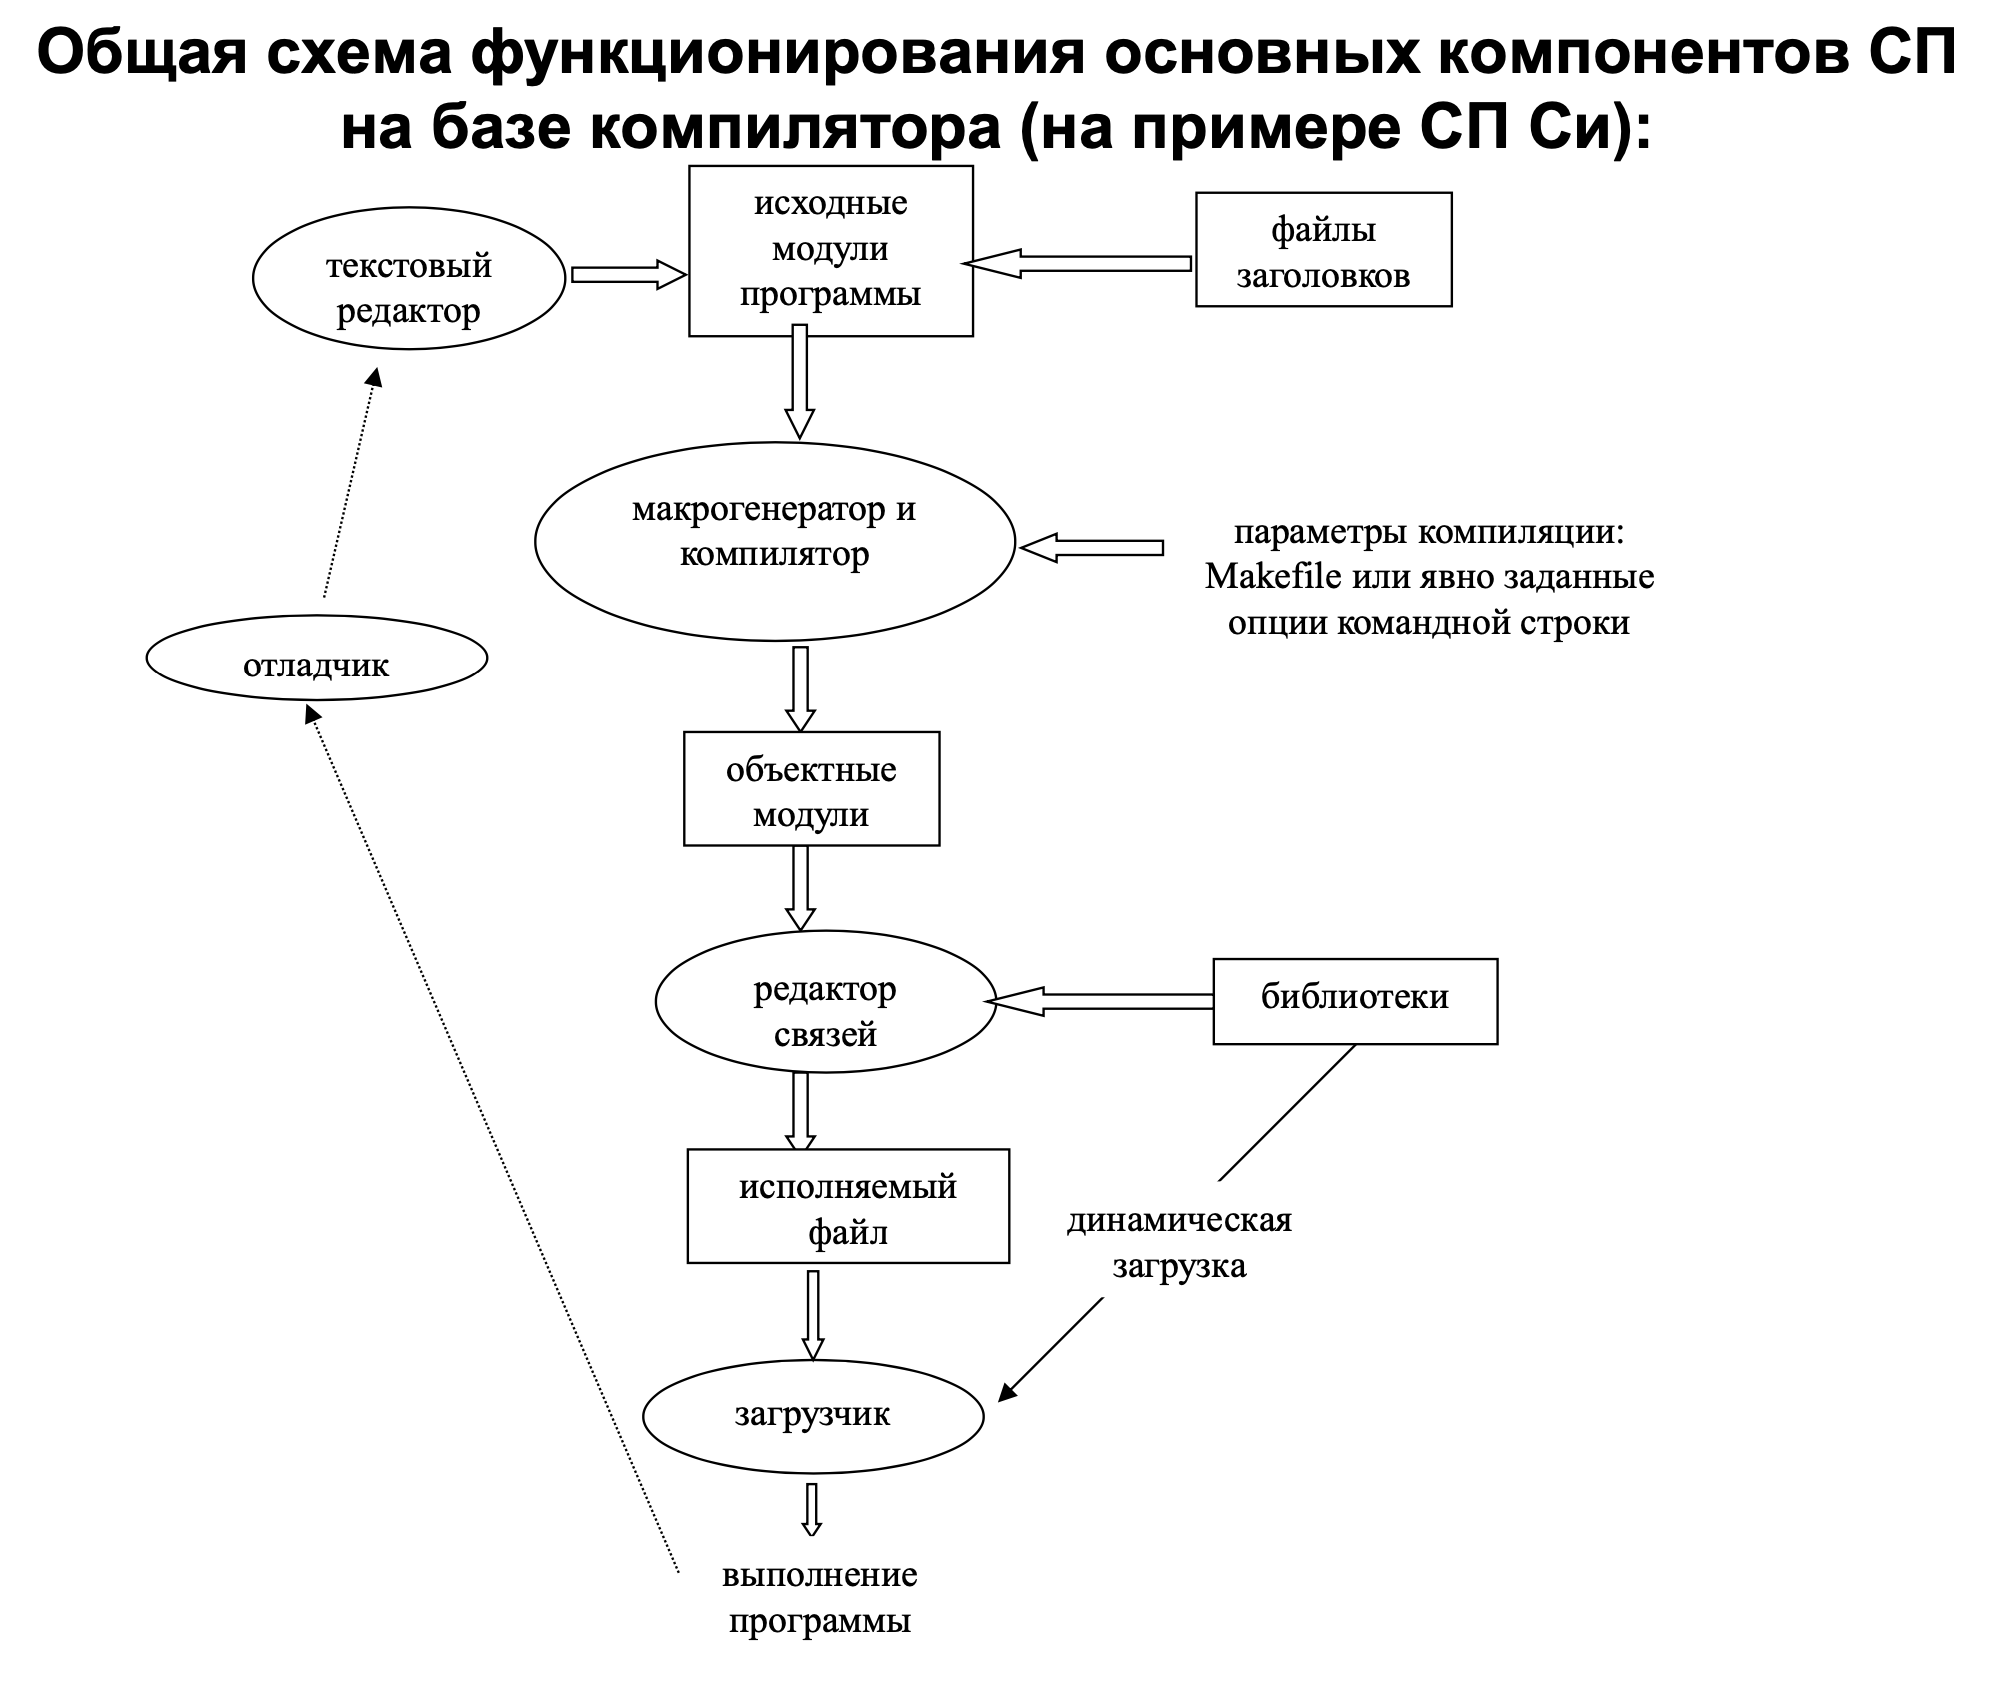
\includegraphics[width=0.5\columnwidth]{pics/scheme_compiler.png}%
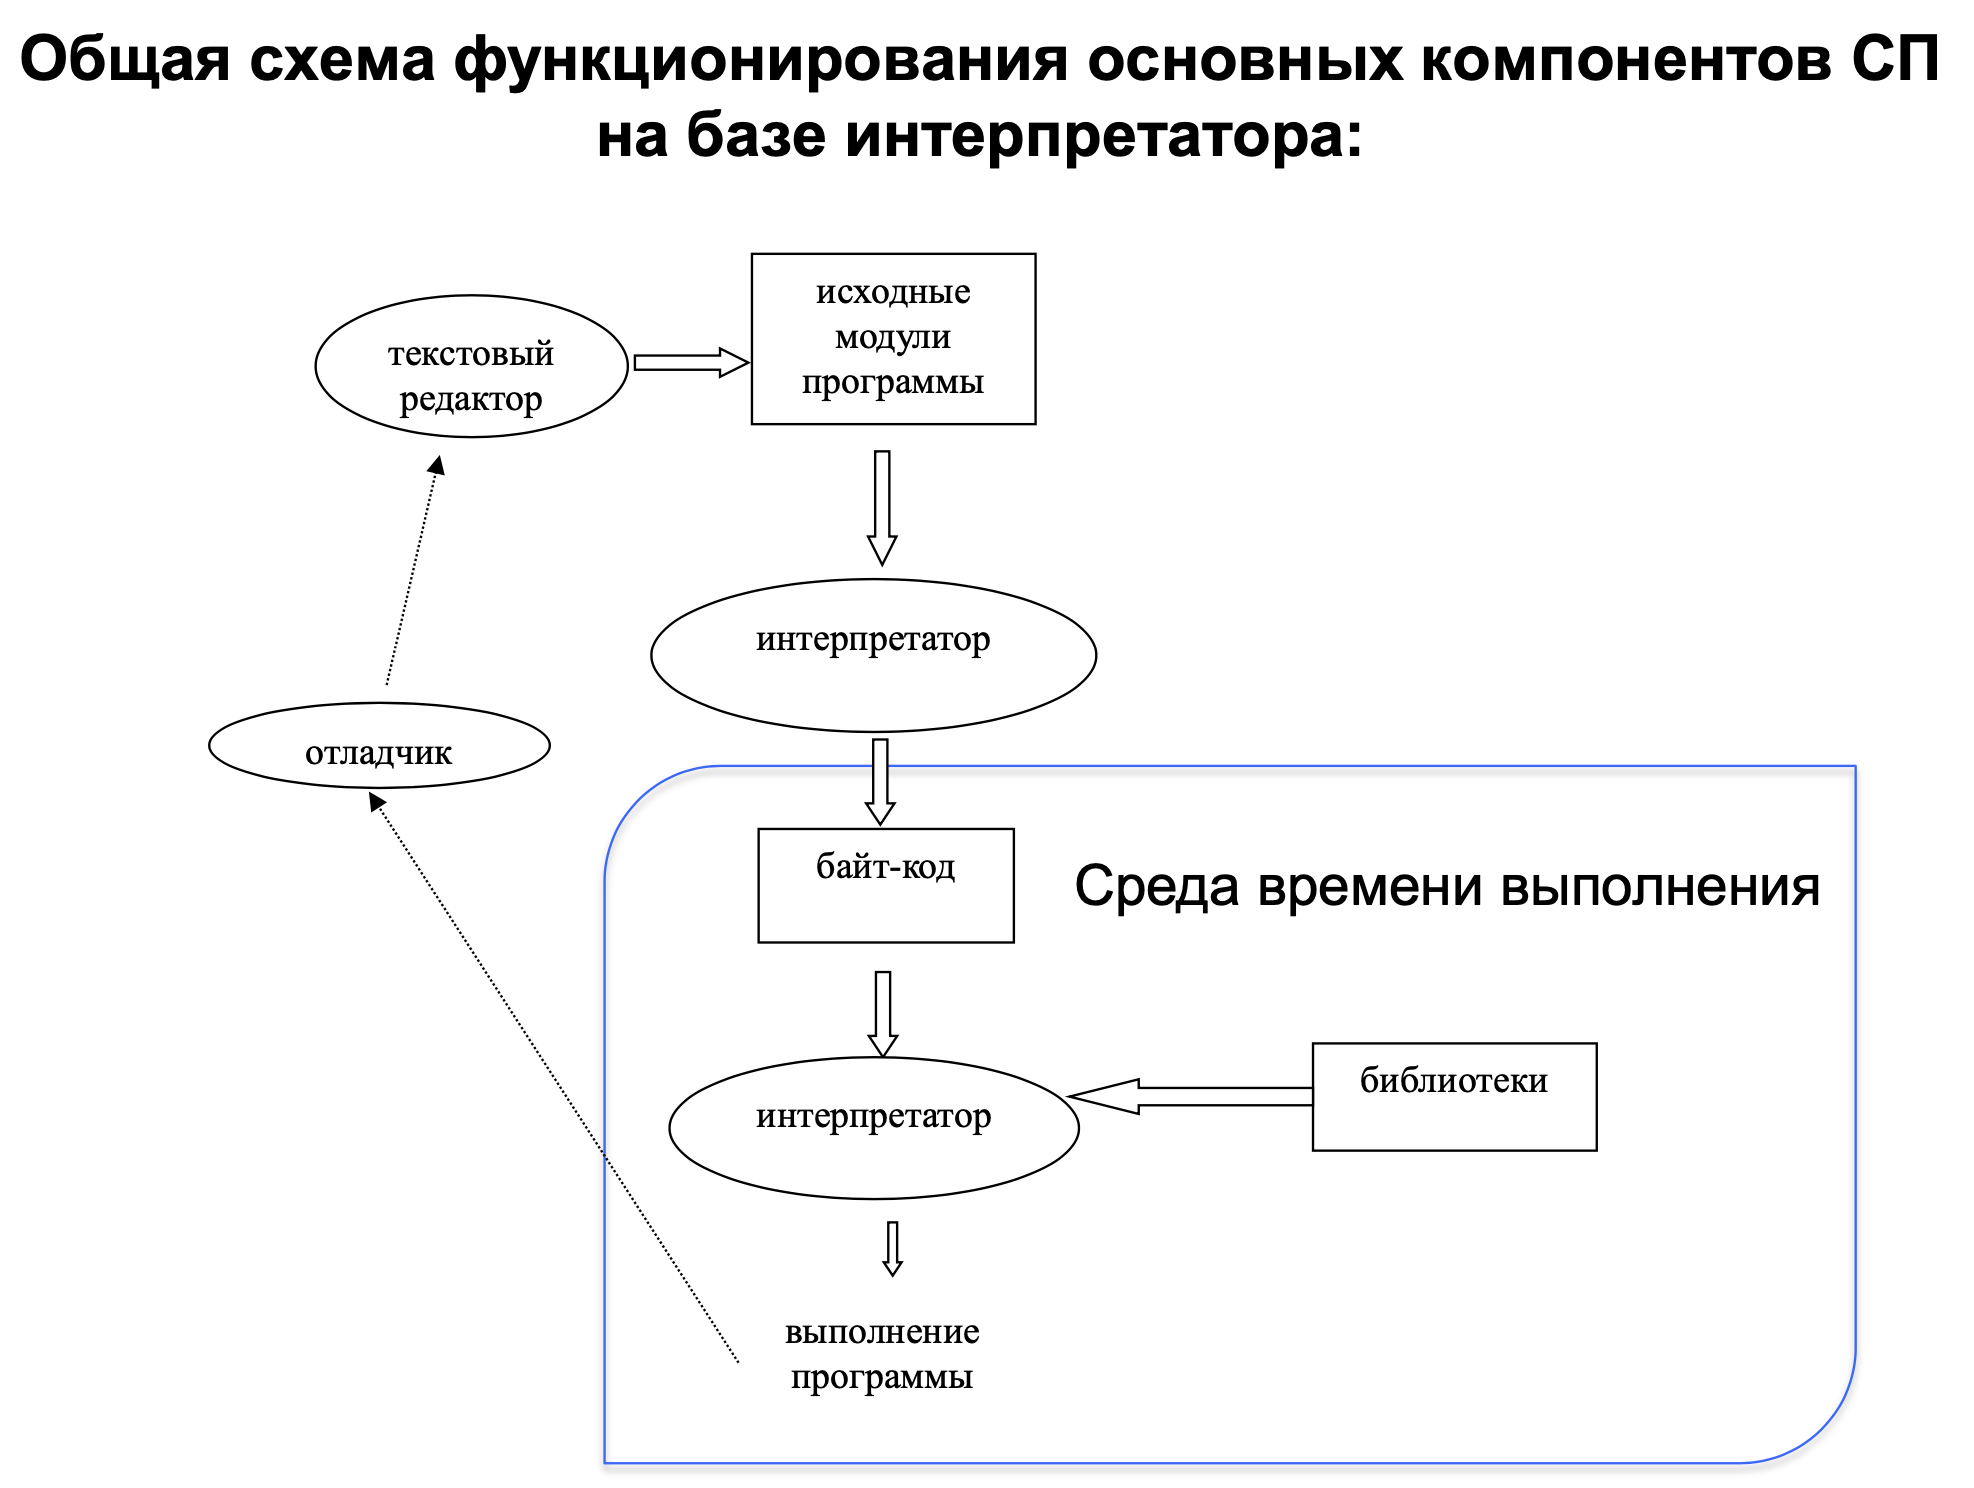
\includegraphics[width=0.5\columnwidth]{pics/scheme_interpret.png}

% -------- source --------
% \bigbreak
% [\cite[page 69-96]{replace_me}]

\vfill\null
\columnbreak
%---------------------2--------------------
\textbf{\LARGE osn 21. Базы данных. Основные понятия реляционной модели данных. Реляционная алгебра. Средства языка запросов SQL.}


\textbf{Основные понятия реляционной модели данных:}

\begin{itemize}
    \item Понятие \textbf{типа данных} в реляционной модели данных полностью соответствует понятию типа данных в языках программирования, состоит из трех основных компонентов: определение множества значений данного типа; определение набора операций, применимых к значениям типа; определение способа внешнего представления значений типа (литералов).
    \item \textbf{Домен} --- допустимое потенциальное, ограниченное подмножество значений данного типа.
    \item Для уточнения термина отношение выделяются понятия заголовка отношения, значения отношения и переменной отношения.
    Пусть дана совокупность типов данных $T_1, T_2, \dots, T_n$, называемых также доменами, не обязательно различных. Тогда $n$-арным \textbf{отношением} $R$, или отношением $R$ степени $n$ называют подмножество декартовa произведения множеств $T_1, T_2, \dots, T_n$.
    \item \textbf{Тело отношения} -- это множество кортежей вида $\{<A_1, T_1, v_1>, < A_2, T_2, v_2 >,\dots, < A_n, T_n, v_n>\}$, где $v_i \in T_i$, $A_i$ -- столбцы (атрибуты) отношения. 

\end{itemize}

\textbf{Алгебра Кодда -- основные реляционные операции}
\begin{itemize}
    \item При выполнении операции \textbf{объединения} (\textit{UNION}) двух отношений производится отношение, включающее все кортежи, входящие хотя бы в одно из отношений-операндов.
    \item Операция \textbf{пересечения} (\textit{INTERSECT}) двух отношений производит отношение, включающее все кортежи, входящие в оба отношения-операнда.
    \item Отношение, являющееся \textbf{разностью} (\textit{MINUS}) двух отношений, включает все кортежи, входящие в отношение-первый операнд, такие, что ни один из них не входит в отношение, являющееся вторым операндом.
    \item При выполнении \textbf{декартова произведения} (\textit{TIMES}) двух отношений производится отношение, кортежи которого являются конкатенацией (сцеплением) кортежей первого и второго операндов.
    \item Результатом \textbf{ограничения} (\textit{WHERE}) отношения по некоторому условию является отношение, включающее кортежи отношения-операнда, удовлетворяющее этому условию.
    \item При выполнении \textbf{проекции} (\textit{PROJECT}) отношения на заданное подмножество множества его атрибутов производится отношение, кортежи которого производятся путем взятия соответствующих значений из кортежей отношения-операнда.
    \item При \textbf{соединении} (\textit{JOIN}) двух отношений по некоторому условию образуется результирующее отношение, кортежи которого являются конкатенацией кортежей первого и второго отношений и удовлетворяют этому условию.
    \item У операции \textbf{реляционного деления} (\textit{DIVIDE BY}) два операнда – бинарное и унарное отношения. Результирующее отношение состоит из унарных кортежей, включающих значения первого атрибута кортежей первого операнда таких, что множество значений второго атрибута (при фиксированном значении первого атрибута) включает множество значений второго операнда.
    \item Операция \textbf{переименования} (\textit{RENAME}) производит отношение, тело которого совпадает с телом операнда, но имена атрибутов могут быть изменены.
    \item Операция \textbf{присваивания} (\textit{:=}) позволяет сохранить результат вычисления реляционного выражения в существующем отношении БД.
\end{itemize}

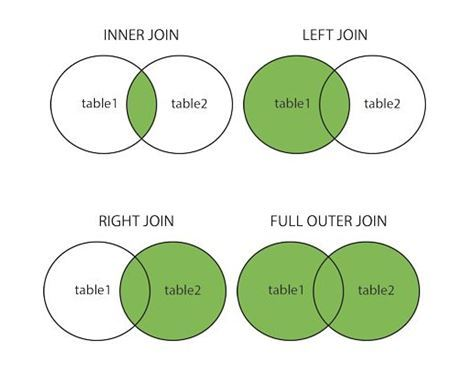
\includegraphics[width=\columnwidth]{pics/osn21_join.jpg}

\textbf{Алгебра Кодда -- специальные реляционные операции}

Имеются важные частные случаи соединения – \textbf{эквисоединение} (\textit{EQUIJOIN}) и \textbf{естественное соединение} (\textit{NATURAL JOIN}).
\begin{itemize}
    \item Операция соединения называется операцией \textbf{эквисоединения}, если условие соединения имеет вид (a = b), где a и b – атрибуты разных операндов соединения.
    \item Пусть AB обозначает объединение заголовков отношений A и B. Тогда \textbf{естественное соединение} A и B – это спроецированный на AB результат эквисоединения A и B по условию A.c = B.c.
\end{itemize}

\textbf{Язык SQL}

\textbf{SQL} --- универсальный компьютерный язык, применяемый для создания, модификации и управления данными в реляционных базах данных.
SQL основывается на реляционной алгебре. Язык SQL представляет собой совокупность операторов, инструкций и вычисляемых функций. Операторы SQL делятся на:
\begin{enumerate}
    \item \textbf{операторы определения данных} (Data Definition Language, DDL):
    \begin{itemize}
        \item[--] \textit{CREATE} создает объект БД (саму базу, таблицу, представление, пользователя и т. д.);
        \item[--] \textit{ALTER} изменяет объект;
        \item[--] \textit{DROP} удаляет объект.
    \end{itemize}
    \item \textbf{операторы манипуляции данными} (Data Manipulation Language, DML):
    \begin{itemize}
        \item[--] \textit{SELECT} считывает данные, удовлетворяющие условиям;
        \item[--] \textit{INSERT} добавляет новые данные;
        \item[--] \textit{UPDATE} изменяет существующие данные;
        \item[--] \textit{DELETE} удаляет данные.
    \end{itemize}
    \item \textbf{операторы определения доступа к данным} (Data Control Language, DCL):
    \begin{itemize}
        \item[--] \textit{GRANT} предоставляет пользователю (группе) разрешения на определенные операции с объектом;
        \item[--] \textit{REVOKE} отзывает ранее выданные разрешения;
        \item[--] \textit{DENY} задает запрет, имеющий приоритет над разрешением.
    \end{itemize}
    \item \textbf{операторы управления транзакциями} (Transaction Control Language, TCL):
    \begin{itemize}
        \item[--] \textit{COMMIT} применяет транзакцию;
        \item[--] \textit{ROLLBACK} откатывает все изменения, сделанные в контексте текущей транзакции;
        \item[--] \textit{SAVEPOINT} делит транзакцию на более мелкие участки.
    \end{itemize}
\end{enumerate}

\textbf{Пример:} Выбрать среднюю зарплату продавцов, которые обслуживают покупателей их штата 'CA'.
\begin{lstlisting}[language=SQL]
    SELECT employee.last_name, employee.salary FROM 
    employee JOIN job using (job_id)
    JOIN customer ON employee_id = salesperson_id 
    WHERE customer.state = 'CA' AND 
    job.function = 'SALESPERSON';
\end{lstlisting}


% -------- source --------
\bigbreak
[\cite{bdbook}]
\vfill\null
\columnbreak
%---------------------3--------------------
% \counterwithin{equation}{chapter} % Use chapter as driver for the resetting


\textbf{\LARGE osn 23. Ансамбли в машинном обучении: комитеты, бэггинг, бустинг, стекинг. Алгоритм градиентного бустинга и его параметры.}  \\
\textbf{Ансамблем} (Ensemble, Multiple Classifier System) называется алгоритм, который состоит из нескольких алгоритмов машинного обучения, а процесс построения ансамбля называется \textbf {ансамблированием} (ensemble learning). Простейший пример ансамбля в регрессии – усреднение нескольких алгоритмов:

\begin{equation}\label{first}
a(x) = \frac{1}{n}(b_1(x)+...+b_n(x))
\end{equation}

Алгоритмы из которых состоит ансамбль (в \ref{first}) называются \textbf{базовыми алгоритмами} (base learners). Если рассматривать значения базовых алгоритмов на объекте  как независимые случайные величины с одинаковым матожиданием  и одинаковой конечной дисперсией, то понятно, что случайная величина \ref{first} имеет такое же матожидание, но меньшую дисперсию:
\begin{equation}
    \xi = \frac{1}{n}(\xi_1+...+\xi_n) 
\end{equation}
\begin{equation}
    \mathbb{E}\xi=\frac{1}{n}(\mathbb{E}\xi_1+...+\mathbb{E}\xi_n)=\mathbb{E}\xi_i
\end{equation}
\begin{equation}
    \mathbb{D}\xi=\frac{1}{n^2}(\mathbb{D}\xi_1+...+\mathbb{D}\xi_n)=\frac{\mathbb{D}\xi_i}{n}
\end{equation}

В задачах классификации простейший пример ансамбля – \textbf{комитет большинства}:
\begin{equation}\label{komitet}
a(x) = mode(b_1(x)+...+b_n(x))
\end{equation}
где  \textbf{mode} – мода (значение, которое встречается чаще других среди аргументов функции). Если рассмотреть задачу классификации с двумя классами {0, 1}  и три алгоритма, каждый из которых ошибается  с вероятностью p, то в предположении, что их ответы – независимые случайные величины, получаем, что комитет большинства этих трёх алгоритмов ошибается с вероятностью $p^2(3-2p)$. Это выражение может быть существенно меньше p  (при p=0.1  почти в два раза), т.е. использование такого ансамбля уменьшает ошибку базовых алгоритмов.

Большинство приёмов в прикладном ансамблировании направлено на то, чтобы ансамбль был «достаточно разнообразным», тогда ошибки отдельных алгоритмов на отдельных объектах будут компенсироваться корректной работой других алгоритмов. По сути, при построении ансамбля:
\begin{itemize}
    \item повышают качество базовых алгоритмов
    \item повышают разнообразие (diversity) базовых алгоритмов
\end{itemize}

\textbf{Бэггинг(Bagging)}
Идея бэггинга (bootstrap aggregating) проста: каждый базовый алгоритм обучается на случайном подмножестве обучающей выборки. В этом случае, даже используя одну модель алгоритмов, мы получаем различные базовые алгоритмы. Есть следующие реализации описанной идеи. \\
\begin{center}
\begin{tabular}{l|l} 
    \hline\hline
    Метод  & Описание \\
     \hline\hline
    Бэгинг  & Подвыборка обучающей выборки \\
     & берётся с помощью бутстрепа \\
     \hline
    Случайные подпространства & Случайное подмножество признаков \\
    (Random Subspaces) & \\
    \hline
    Случайные патчи & Одновременно берём случайное подмножество \\
    (Random Patches) & объектов и признаков

 \end{tabular}
\end{center}

Бэгинг позволяет получать т.н. out-of-bag(OOB)-ответы модели. Идея очень простая: каждый алгоритм обучается на подвыборке, в неё, вообще говоря, попадают не все объекты их обучения, поэтому на остальных объектах можно узнать ответы алгоритма. При достаточном числе базовых алгоритмов мы таким образом оцениваем ответ почти на всех объектах обучения. При этом это «честный» ответ: те алгоритмы, которые участвовали в его формировании «не видели» истинной метки соответствующего объекта.

Аналогично оценивается out-of-bag(OOB)-ошибка бэгинга. Можно оценить ошибку с помощью полученных  OOB-ответов, но чаще делают проще: для каждого базового алгоритма ошибку оценивают на объектах, не попавших в его обучение, а затем ошибки усредняют.

\textbf{Бустинг (Boosting)}
Главная идея бустинга – базовые алгоритмы строятся не независимо, каждый следующий мы строим так, чтобы он исправлял ошибки предыдущих и повышал качество всего ансамбля. Первый успешный вариант бустинга – AdaBoost (Adaptive Boosting), сейчас практически не используется, поскольку его вытеснил градиентный аналог. Основной принцип реализации бустинга – Forward stagewise additive modeling (FSAM). Пусть, например, решается задача регрессии с функцией ошибки $L(y, a)$. Предположим, мы уже построили алгоритм a(x), теперь строим b(x) таким образом, чтобы
\begin{equation}
    \displaystyle\sum_{i=1}^{m} L(y_i, a(x_i) + b(x_i)) \xrightarrow{} min
\end{equation}
где $y_i$ - истинная метка, $x_i$-признаки i-го объекта выборки.
Особенность терминологии, когда говорят о бустинге следующая. Базовые алгоритмы называются \textbf{«слабыми»} (weak learners),  а ансамбль – \textbf{«сильным»} алгоритмом (strong learner).

\textbf{Стекинг (stacking)} — алгоритм ансамблирования, основные свойства:
\begin{itemize}
    \item он может использовать алгоритмы разного типа, а не только из какого-то фиксированного семейства. Например, в качестве базовых алгоритмов могут выступать метод ближайших соседей и линейная регрессия
    \item результаты базовых алгоритмов объединяются в один с помощью обучаемой мета-модели, а не с помощью какого-либо обычного способа агрегации (суммирования или усреднения)
\end{itemize}
Простейшая схема стекинга — \textbf{блендинг} (Blending): обучающую выборку делят на две части. На первой обучают базовые алгоритмы. Затем получают их ответы на второй части и на тестовой выборке. Понятно, что  ответ каждого алгоритма можно рассматривать как новый признак (т.н. «метапризнак»). На метапризнаках второй части обучения настраивают метаалгоритм. Затем запускают его на метапризнаках теста и получают ответ.

\textbf{Градиентный бустинг и его параметры} \\
Предположим, что решается задача машинного обучения (для простоты можно считать, что регрессии) с обучающей выборкой $(x_i, y_i), i=1,...,m$, и дифференцируемой функцией ошибки $L(y, a)$. Мы построили алгоритм $a(x)$, давайте теперь построим алгоритм $b(x)$ такой, что
\begin{equation}\label{sum a and b}
    a(x_i)+b(x_i)=y_i, i \in \{1,2,...m\}.
\end{equation}
Такой алгоритм осуществляет поправку ответов алгоритма $a(x)$ до верных ответов на обучающей выборке, т.е. на невязку $\varepsilon_i = y_i - a(x_i)$. 
Главный вопрос здесь – как обучить второй алгоритм. Вообще говоря, нельзя считать, что мы получили новую задачу с обучающей выборкой $(x_i, \varepsilon_i), i=1,...,m$ и функцией ошибки $L(y, a)$, поскольку наша задача 
\begin{equation}\label{1}
    \displaystyle\sum_{i=1}^{m} L(y_i, a(x_i) + b(x_i)) \xrightarrow{} min
\end{equation}
может отличаться от решения
\begin{equation}\label{2}
    \displaystyle\sum_{i=1}^{m} L(y_i - a(x_i), b(x_i)) \xrightarrow{} min
\end{equation}
Хотя, справедливости ради, заметим, что для большинства разумных функций ошибок записи \ref{1} и \ref{2} эквивалентны. \\
Не всегда \ref{1} решается аналитически (из-за достаточно сложных функций ошибок). Перепишем \ref{1} в таком виде 
\begin{equation}\label{3}
    F = \displaystyle\sum_{i=1}^{m} L(y_i, a(x_i) + b_i) \xrightarrow{} \min_{(b_1, ..., b_m)}
\end{equation}
если рассматривать эту задачу как задачу минимизации функции $F(b_1, ..., b_m)$, то полезно вспомнить, что функция многих переменных максимально убывает в направлении своего антиградиента: 
\begin{equation}\label{4}
    -(L'(y_1, a(x_1)),..., L'(y_m, a(x_m))),
\end{equation}
здесь производная берётся по второму аргументу. Получается, что выгодно считать
\begin{equation}\label{5}
    b_i = -(L'(y_i, a(x_i))), i \in \{1,2,...m\},
\end{equation}
а это и есть ответы нашего алгоритма b. Получается, что его следует настраивать на обучающей выборке 
\begin{equation}\label{6}
   (x_i, -L'(y_i, a(x_i))), i \in \{1,2,...m\},
\end{equation}
Из выражения \ref{6} понятно будет название – градиентный бустинг. 
Итак, мы научились строить алгоритм b, который корректирует ответы алгоритма a. Понятно, что и сумма этих алгоритмов может иметь значительную ошибку, но можно построить третий алгоритм, который корректирует эту сумму. Процесс построения можно продолжить. Получаем классический алгоритм градиентного бустинга. \\


Перечислим \textbf{параметры градиентного бустинга} в современных реализациях:
\begin{itemize}
    \item Параметры, определяющие задачу: \\
        -objective – какая задача решается и в каком формате будет ответ \\
        -loss – функция ошибки для минимизации \\
        -eval\_metric – значения какой функции ошибки смотреть на контроле \\
    \item Параметры, определяющие тип бустинга и способы построения деревьев: \\
    --booster – какой бустинг проводить: над решающими деревьями или линейный \\
    -grow\_policy – порядок построения дерева: на следующем шаге расщеплять вершину, ближайшую к корню, или на которой ошибка максимальна\\
    -init – какой алгоритм использовать в качестве первого базисного (именно его ответы будет улучшать бустинг). 
    \item Основные параметры: \\
    -learning\_rate – темп (скорость) обучения \\
    -num\_iterations / n\_estimators  – число итераций бустинга \\
    -early\_stopping\_round  –  если на отложенном контроле заданная функция ошибки не уменьшается такое число итераций, обучение останавливается
    \item Параметры регуляризации
    
    
\end{itemize}


Ссылки на используемые материалы:
\begin{itemize}
    \item \href{https://alexanderdyakonov.wordpress.com/2019/04/19/%D0%B0%D0%BD%D1%81%D0%B0%D0%BC%D0%B1%D0%BB%D0%B8-%D0%B2-%D0%BC%D0%B0%D1%88%D0%B8%D0%BD%D0%BD%D0%BE%D0%BC-%D0%BE%D0%B1%D1%83%D1%87%D0%B5%D0%BD%D0%B8%D0%B8}{Ансамбли в машинном обучении, сайт Дьяконова}
    \item \href{https://academy.yandex.ru/handbook/ml/article/ansambli-v-mashinnom-obuchenii}{Ансамбли в машинном обучении, учебник по машинному обучению Яндекса}
    \item \href{https://alexanderdyakonov.wordpress.com/2017/03/10/c%d1%82%d0%b5%d0%ba%d0%b8%d0%bd%d0%b3-stacking-%d0%b8-%d0%b1%d0%bb%d0%b5%d0%bd%d0%b4%d0%b8%d0%bd%d0%b3-blending/}{Стеккинг, Блендинг, сайт Дьяконова}
    \item \href{http://dyakonov.org/2017/06/09/%d0%b3%d1%80%d0%b0%d0%b4%d0%b8%d0%b5%d0%bd%d1%82%d0%bd%d1%8b%d0%b9-%d0%b1%d1%83%d1%81%d1%82%d0%b8%d0%bd%d0%b3/}{ГРАДИЕНТНЫЙ БУСТИНГ, Дьяконов}
\end{itemize}



\vfill\null
\columnbreak
%---------------------
\end{multicols}
\end{tcolorbox}
% --- END OF PAGE ----



% --- BEGIN OF PAGE ----
\newpage
\begin{tcolorbox}[colback=white, left=0mm, right=0mm]
\begin{multicols}{4}
%---------------------0--------------------
% \input{tickets/t_osn24}
\vfill\null
\columnbreak
%---------------------1--------------------
\textbf{\LARGE osn 22. Виды параллельной обработки данных, их особенности. Компьютеры с общей и распределенной памятью. Производительность вычислительных систем, методы оценки и измерения.}


Параллельная обработка данных имеет две разновидности: конвейерность и параллельность.
\begin{itemize}
    \item \textbf{Параллельная обработка.} Увеличение количества независимо работающих устройств. Если некое устройство выполняет одну операцию за единицу времени, то тысячу операций оно выполнит за тысячу единиц. Система из N устройств ту же работу выполнит за 1000/N единиц времени (в идеальном случае).
    \item \textbf{Конвейерная обработка.} Усложнение самого устройства, чтобы на разных этапах могли находиться разные данные. Идея заключается в выделении отдельных этапов выполнения общей операции, причем каждый этап, выполнив свою работу, передавал бы результат следующему, одновременно принимая новую порцию входных данных. Получаем выигрыш в скорости обработки за счет совмещения прежде разнесенных во времени операций. Существует некоторая задержка (время разгона), для того, чтобы заполнить все этапы конвейера; когда он заполнен, происходит ускорение обработки.
\end{itemize}

\textbf{Классификация многопроцессорных сетей по Флинну.}

В контексте машины можно выделить два потока информации: \textbf{поток управления} (для передачи управляющих воздействий на конкретное устройство) и \textbf{поток данных} (циркулирующий между оперативной памятью и внешними устройствами). В связи с этим выделяют 4 основных класса: SISD (1 поток команд, 1 поток данных. ``Традиционный'' последовательный компьютер), SIMD (1 поток команд, много потоков данных, пример - векторные компьютеры), MISD (много п. ком., 1 п. данных), MIMD (много и потоков команд, и данных). Среди MIMD можно выделить системы с общей ОП и системы с распределенной памятью.

\begin{itemize}
    \item \textbf{Компьютеры с общей памятью.}
    
    В системе присутствует несколько равноправных процессоров, имеющих одинаковый доступ к единой памяти. Всё, кроме процессоров, в одном экземпляре: образ операционной системы, память, подсистема ввода-вывода и т.д. Все процессоры работают с единым адресным пространством. (+) относительная простота параллельного программирования; (–) сложность увеличения числа процессоров (роста производительности).
    
    \textbf{UMA} -- системы с однородным доступом к памяти (все процессоры имеют одинаковый доступ к памяти). SMP --- есть общая шина, соединенная со всеми процессорами и с ОП.
    
    \textbf{NUMA} (Non Uniform Memory Access) -- память физически распределена, но логически общедоступна. Каждый вычислительный узел компьютера содержит процессор, локальную память, контроллер памяти и, быть может, некоторые устройства ввода/вывода. Контроллер памяти определяет, является ли запрос к памяти локальным или его необходимо передать удаленному узлу через коммутатор/шину. Проблема -- синхронизация кэш. 
    
    \textbf{ccNUMA} (cache coherent NUMA). На аппаратном уровне решает проблему когерентности кэшей. Но остаются ограничения, связанные с централизацией -- использованием системной шины, возникают ограничения, связанные с cc-архитектурой: есть системные потоки служебной информации, что ведет к дополнительным накладным расходам --- загрузке общей шины служебной информацией
    
    \item \textbf{Компьютеры с распределенной памятью.}
    
    Состоят из вычислительных узлов, каждый из которых является полноценным компьютером со своей памятью, ОС, устройствами ввода-вывода и т.п., взаимодействующих друг с другом через коммуникационную среду.
    (–) сложность параллельного программирования;
    (+) относительная простота увеличения числа процессоров (роста производительности).
\end{itemize}

\textbf{Основные понятия для распределённых систем}
\begin{itemize}
    \item \textbf{Длина критического пути} -- минимальное количество элементарных связей, которые нужно пройти для коммутации двух самых удаленных процессоров. \todo{что такое коммутация процессов?}
    \item \textbf{Связность} -- минимальное количество элементарных связей, которые нужно удалить, чтобы схема распалась на две несвязанные части.
    \item \textbf{Сложность} --- общее количество необходимых элементарных связей. 
    \item \textbf{Латентность и пропускная способность сети} – основные параметры коммуникационной сети кластеров. 
    
    \textbf{Латентность} --- время начальной задержки при посылке сообщений. 
    
    \textbf{Пропускная способность сети} определяется скоростью передачи информации по каналам связи и измеряется объёмом передаваемой информации в единицу времени. Время на передачу сообщения по коммуникационной сети вычисляется по следующей формуле: $t_N = t_0 + \frac{N}{S}$ , где $t_0$ -- латентность, $N$ -- объём передаваемых данных, $S$ -- пропускная способность сети.
\end{itemize}

\resizebox{\columnwidth}{!}{
\begin{tabular}{ |c|c|c|c| } 
    \hline
    Схема коммутации & Длина критического пути & Связность & Сложность \\ 
    \hline\hline
    линейка & $p - 1$  & $1$ & $p - 1$ \\ 
    \hline
    кольцо & $|\frac{p}{2}|$ & $2$ & $p$ \\
    \hline
    звезда & $2$ & $1$ & $p - 1$ \\
    \hline 
    полносвязная топология & $1$ & $p - 1$ & $ \frac{p(p-1)}{2}$\\
    \hline
\end{tabular}
}
\begin{center}
    $p$ -- количество процессов
\end{center}

\textbf{Методы оценки производительности.}
\begin{itemize}
    \item \textbf{Пиковая производительность} -- теоретический предел производительности для данного компьютера. Пиковая производительность компьютера вычисляется как сумма пиковых производительностей всех входящих в него вычислительных устройств (процессоров, ускорителей и т.д.). Даёт нижнюю оценку времени выполнения программы. Производительность компьютера на любой реальной программе никогда не только не превысит этого порога, но и не достигнет его точно.
    \item \textbf{Реальная производительность} -- производительность данного компьютера на конкретном приложении. Традиционно используются два способа оценки производительности компьютера. Один из них опирается на число команд, выполняемых компьютером в единицу времени. Единица измерения -- \textbf{MIPS} (Million Instructions Per Second). Второй способ -- число вещественных операций, выполняемых компьютером в единицу времени -- \textbf{Flops} (Floating point operations per second).
    
    Популярные тесты: 
    \item[--] \textbf{LINPACK}: измерение производительности при обработке чисел с плавающей точкой. Задача: решение СЛАУ.
    \item[--] \textbf{Graph500}: нагружает коммуникационную систему компьютера и не зависит от количества исполняемых в секунду операций с числами с плавающей точкой. Задача: поиск в ширину в большом ненаправленном графе.
    \item[--] \textbf{NAS Parallel Benchmark}: набор различных задач для проверки производительности.
\end{itemize}



% % -------- source --------
% \bigbreak
% [\cite[page 69-96]{replace_me}]
\vfill\null
\columnbreak
%---------------------2--------------------
\textbf{\LARGE osn 20. Основные принципы объектно-ориентированного программирования. Реализация этих принципов в языке С++. Примеры.}


\centerline{\textbf{Основные механизмы (постулаты) ООП:}}

1. \textbf{Инкапсуляция} -- это \textit{механизм}, который связывает данные с обрабатывающими их кодами и защищает и те, и другие от внешних воздействий и ошибочных действий. В объектно-ориентированном языке коды и данные могут быть связаны так, что вместе они создают автономный \textit{черный ящик}. Внутри этого ящика содержатся все необходимые данные и коды. При связывании таким образом данных и кодов создается \textit{объект}. Другими словами, объект представляет собой устройство, поддерживающее инкапсуляцию.
    
Внутри объекта коды или данные или и те, и другие могут иметь атрибут \textit{private}, что делает их закрытыми для внешнего мира, или \textit{public}, что открывает эти элементы объекта. Закрытые коды и данные известны и доступны только из других частей того же объекта. Другими словами, к закрытым кодам и данным нельзя обратиться ни из какого фрагмента программы, существующего вне объекта. Если же код или данные объявлены с атрибутом public, то доступ к ним открыт из любых частей программы, несмотря на то, что эти элементы определены внутри объекта. Обычно открытые элементы объекта используются для обеспечения контролируемого интерфейса с закрытыми элементами того же объекта.
    
В С++ базовой единицей инкапсуляции является \textbf{класс}. Класс определяет содержание объекта. Класс описывает как данные, так и коды, предназначенные для операций над этими данными. С++ использует спецификацию класса при конструировании \textit{объектов}. Объекты являются экземплярами класса. Т.е. класс в сущности представляет собой набор чертежей, по которым строится объект.
    
Код и данные, составляющие класс, называются \textit{членами} класса. Конкретно, \textit{члены-переменные}, называемые также переменными экземпляра, -- это данные, определенные в классе. \textit{Члены-функции}, или просто функции -- это коды, предназначенные для операций над данными.
    
2. \textbf{Полиморфизм} обозначает средство, позволяющее посредством единого интерфейса получить доступ к целому классу действий. Простым примером полиморфизма может служить рулевое колесо автомобиля. Рулевое колесо (интерфейс) остается одним и тем же, независимо от того, какой тип рулевого механизма используется в данном автомобиле. Другими словами, рулевое колесо действует одинаково для любых автомобилей: с непосредственным приводом на колеса, с гидравлическим усилителем или с реечной передачей. Поворот рулевого колеса влево заставляет автомобиль двигаться влево независимо от типа рулевого механизма. Достоинство единого интерфейса, очевидно, заключается в том, что если вы умеете пользоваться рулевым колесом, вы можете ездить на любых автомобилях.
    
Рассмотрим стек (список, действующий по правилу “первым вошел, последним вышел”). Пусть вашей программе требуется три стека различных видов. Один стек используется для целых чисел, другой для чисел с плавающей точкой, а третий для одиночных символов. Алгоритм реализации всех трех стеков будет одинаков, несмотря на то, что данные, заносимые в разные стеки, различаются. 
    
В общем случае концепция полиморфизма часто выражается фразой “один интерфейс, много методов”. Это означает возможность разработать обобщенный интерфейс для группы схожих действий.
    
Различают \textbf{статический} (реализуется на этапе компиляции с помощью перегрузки функций и операций), \textbf{динамический} (реализуется во время выполнения программы с помощью механизма виртуальных функций) и \textbf{параметрический} (реализуется на этапе компиляции с использованием механизма шаблонов) полиморфизм.
    
3. \textbf{Наследование} является процессом, который позволяет одному объекту приобретать свойства другого объекта. Важность наследования определяется тем, что оно поддерживает концепцию иерархической классификации. Большая часть наших знаний построена по иерархическому принципу. Например, антоновка является частью класса яблок, который, в свою очередь, есть часть класса фруктов; фрукты же входят в более широкий класс пищевых продуктов. Класс пищевые продукты обладает определенными качествами (съедобность, пищевая ценность и т. д.), которые, логично предположить, приложимы и к его подклассу фрукты. В дополнение к этим качествам класс фрукты обладает специфическими характеристиками (сочность, сладость и др.), которые выделяют его среди других пищевых продуктов. Класс яблоки определяет качества, характерные для яблок (растут на деревьях, не являются тропическими продуктами и т. д.). Класс антоновка, в свою очередь, наследует все качества всех предшествующих классов и определяет лишь те качества, которые выделяют антоновку среди прочих яблок.
    
Если не пользоваться иерархией, то каждый объект должен был бы явно определять все свои характеристики. При использовании же наследования объект определяет лишь те качества, которые делают его уникальным в рамках его класса. Более общие качества он может наследовать от родительского класса. Таким образом, механизм наследования позволяет объекту быть специфическим экземпляром более общего класса.

\centerline{\textbf{Примеры на C++:}}
1. \textbf{Инкапсуляция}.
Пример класса <<\textit{коробка}>>, инкапсулирующего данные и предоставляющего метод для вычисления объема.

\begin{lstlisting}[language=C++]
class Box { 
    int length;
    int width;
    int height; 
public:
    int volume() const {
        return length * width * height;
    }
}
\end{lstlisting}

2. \textbf{Наследование}.
Наследование свойств и поведения могут контролироваться с помощью квалификаторов доступа, задаваемых при наследовании: \textit{public, protected, private}.  В примере ниже класс C является наследником класса A.

\begin{lstlisting}[language=C++]
class A { 
public:
    virtual void f(int x) { 
        cout << "A::f" << '\n';
    }
};

class C: public A {
public:
    void f(int x) {
        cout << "C::f" << '\n';
    }
};
\end{lstlisting}

3. \textbf{Полиморфизм.}

\textbf{Статический полиморфизм} реализуется с помощью перегрузки функций и операций. Под перегрузкой функций в С++ понимается описание в одной области видимости нескольких функций с одним и тем же именем.
\begin{lstlisting}[language=C++]
void f(int x);
void f(double x);
\end{lstlisting}
\textbf{Динамический полиморфизм} реализуется с помощью механизма виртуальных методов.
Механизм виртуальных методов заключается в том, что результат вызова виртуального метода с использованием указателя или ссылки зависит не от того, на основе какого типа создан указатель, а от типа объекта, на который он указывает. Тип данных (класс), содержащий хотя бы одну виртуальную функцию, называется \textbf{полиморфным типом (классом)}, а объект этого типа – \textbf{полиморфным объектом}. Во всех наследниках виртуальная функция остается таковой.

В примере ниже используются описанные выше классы A и C.
\begin{lstlisting}[language=C++]
int main() { 
    A a1;
    C c1;
    C *pc = &c1;
    pc->f(1); // C::f
    A *pa = pc;
    pa->f(1); // C::f
    pc = (C*) &a1;
    pc->f(1); // A::f
    return 0;
}
\end{lstlisting}
\textbf{Чистая виртуальная функция} --- функция вида: \\
\textit{virtual <тип\_возвращаемого\_значения> имя\_функции (формальные\_параметры) = 0;}

Такая форма записи функции означает, что данная функция (точнее, метод класса) не имеет тела, описывающего ее алгоритм.

\textbf{Абстрактный класс} --- это класс, содержащий хотя бы одну чистую виртуальную функцию.

\textbf{Параметрический полиморфизм} позволяет применить один и тот же алгоритм к разным типам данных. При этом тип является параметром тела алгоритма. При обращении к функции-шаблону после имени функции в угловых скобках указываются фактические параметры шаблона -- имена реальных типов или значения объектов.
\begin{lstlisting}[language=C++]
template <class T> T max(T &x, T &y) {
    return x > y ? x : y; 
}
\end{lstlisting}

% -------- source --------
\bigbreak
[\cite[page 20-23]{gerbert}]
\vfill\null
\columnbreak
%---------------------3--------------------
\textbf{\LARGE osn 18. Операционные системы. Процессы, взаимодействие процессов, разделяемые ресурсы, синхронизация взаимодействующих процессов, взаимное исключение. Программирование взаимодействующих процессов с использованием средств ОС UNIX (сигналы, неименованные каналы, IPC).}

\textbf{Операционная система} --- комплекс программ, используемых для управления ресурсами компьютера и предоставления интерфейса пользователю.
В понятие управление ресурсами входит \textit{выделение} ресурсов для программ (например, памяти и процессорного времени),
\textit{защита} от доступа программ к ресурсам, которыми они не владеют, а также
\textit{абстрагирование} от оборудования, например, предоставление общего интерфейса для похожих типов устройств
(общий файловый интерфейс для всех дисков) или реализация виртуальных ресурсов (увеличение эффективного объема памяти за счет файла подкачки).

\textbf{Физические ресурсы (устройства)} -- компоненты аппаратуры компьютера, используемые на программных уровнях ВС или оказывающие влияние на функционирование всей ВС. Совокупность физических ресурсов составляет аппаратный уровень вычислительной системы.

\textbf{Логические, или виртуальные ресурсы (устройства) ВС} -- устройство/ресурс, некоторые эксплуатационные характеристики которого (возможно все) реализованы программным образом.

\textbf{Состав ОС:} 
\begin{itemize}
    \item ядро ОС - резидентная часть ОС, реализующая некоторую базовую функциональность ОС и работающая в режиме супервизора;
    \item динамически подгружаемые драйверы физических и виртуальных устройств. под динамически подгружаемыми понимается то, что в зависимости от ситуации состав этих драйверов при инсталяции и загрузке системы может меняться;
    \item интерфейсы системных вызовов.
\end{itemize} 

\textbf{Типы ОС:} 

- Пакетные ос  - система, критерием эффективности которой является максимальная загрузка ЦП. Время работы процессора/время работы исполнения пользовательских программ ~ 1. Пакет программ - совокупность программ которые системе необходимо обработать. Переключение процессов происходит по 1 из трех причин: зацикливание процесса, завершение процесса, обращение к внешнему устройству. 

- ОС разделения времени - модель, представляющая собой развитие пакетных систем. Дополнительная характеристика - квант процессорного времени - некоторый фиксированный ос промежуток времени работы процессора. + причина по смене исполняемого процесса - исчерпание кванта времени. 

- ОС реального времени - системы, ориентированные на обработку некоторого фиксированного набора событий, при возникновении любого из которых гарантируется обработка этого события за некоторый промежуток времени, не превосходящий определенного предельного значения. 

- Сетевые ОС - ос, обеспечивающая функционирование и взаимодействие вычислительной системы в пределах сети. 

- Распределенная система - система, функционирующая на многопроцессорном/многомашинном комплексе, в котором на каждом из узлов функционирует отдельное ядро, а сама система обеспечивает реализацию распределенных возможностей ОС. 

Под \textbf{процессом} понимается совокупность машинных команд и данных, обрабатываемая в вычислительной системе и обладающая правами на владение некоторым набором ресурсов ВС. \textbf{Процесс (полновесный)} - объект планирования и выполняется внутри защищённой области памяти. \textbf{Легковесные процессы} - могут активироваться внутри полновесного процесса, могут быть объектами планирования, и при этом они могут функционировать внутри общей (т.е. незащищённой от других нитей) области памяти. Понятие процесса включает в себя следующее:исполняемый код, собственное адресное пространство, представляющее собой множество виртуальных адресов, которые может использовать процесс, ресурсы сиcтемы, которые назначены процессу ос, хотя бы одну выполняемую нить. 
\textbf{Системный вызов} - средство ос, предоставляемое пользователям (процессам), посредством которого процессы могут обращаться к ядру ос за выполнением тех или иных функций.
\textbf{Процесс} - объект, порожденный системным вызовом \textbf{fork}. 
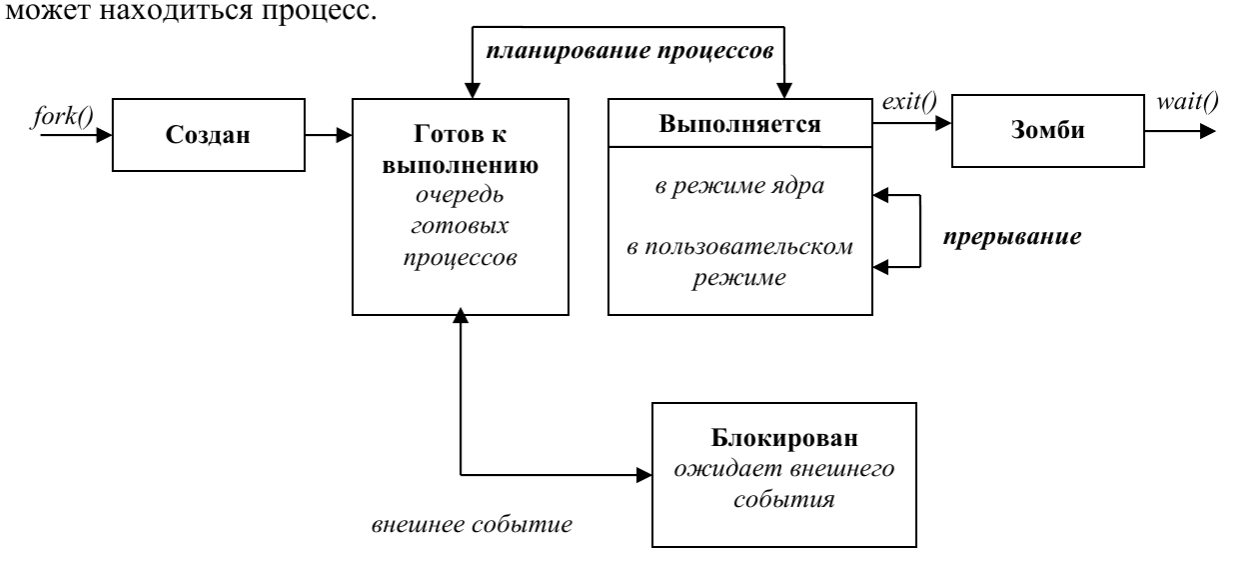
\includegraphics[scale=0.27]{pics/life_cycle.png}

Будем говорить, что процессы называются \textbf{параллельными}, если их выполнение хотя бы частично перекрывается по времени.
Совместное использование ресурса ВС двумя и более параллельными процессами, когда каждый некоторое время владеет этим ресурсом, называется \textbf{разделением ресурса.} Ситуация, когда процессы конкурируют за разделяемый ресурс, называются \textbf{гонкой процессов}. \textbf{Критический ресурс} - разделяемый ресурс, который в каждый момент времени доступен только одному из взаимодействующих процессов.  

\textbf{Пример.} Имеется разделяемый ресурс \textit{in} и два процесса. В некоторый момент времени процесс $A$ присвоил переменной \textit{in} значение $X$. Затем в некоторый момент процесс $B$ присвоил значение $Y$ этой же переменной \textit{in}. Далее оба процесса читают эту переменную, и в обоих случаях процессы прочтут значение $Y$ . То есть символ, считанный процессом $A$, был потерян, а символ, считанный процессом $B$, был выведен дважды. Результат выполнения процессов здесь зависит от того, в какой момент осуществляется переключение процессов, и от того, какой конкретно процесс будет выбран следующим для выполнения.

\textbf{Взаимное исключение} - способ работы с разделяемым ресурсом, при котором когда один из процессов работает с разделяемым ресурсом, все остальные не могут иметь к нему доступ.

\textbf{Блокировка} - доступ к разделяемому ресурсу одного из взаимодействующих процессов не обеспечивается из-за активности более приоритетных.

\textbf{Тупик} - взаимоблокировка.

\textbf{Семафоры Дейкстры}

Имеется специальный тип данных --- \textit{семафор}. Переменные типа семафор могут принимать целочисленные значения. Определены атомарные операции: опустить семафор \textit{down(S)} (или \textit{P(S)}) и поднять семафор \textit{up(S)} (или \textit{V(S)}).

Операция \textit{down(S)} проверяет значение семафора \textit{S} и, если оно больше нуля, то уменьшает его на 1. Если же это не так, процесс блокируется, причем связанная с заблокированным процессом операция down считается незавершенной.

Операция \textit{up(S)} увеличивает значение семафора на 1. При этом если в системе присутствуют процессы, блокированные ранее при выполнении \textit{down} на этом семафоре, то один из них разблокируется и завершает выполнение операции \textit{down}, т.е. вновь уменьшает значение семафора. Выбор процесса для разблокирования никак не оговаривается. Используется для предотвращения тупика. 

\textbf{Монитор} - это языковая конструкция с централизованным управлением (в отличие от семафоров, которые не обладают централизацией).
\begin{enumerate}
    \item Cтруктуры данных монитора доступны только через обращения к процедурам или функциям этого монитора (т.е. монитор представляет собой некоторый аналог объекта в объектно-ориентированных языках и реализует инкапсуляцию данных);
    \item процесс занимает (или входит в) монитор, если он вызывает одну из процедур или функций монитора;
    \item В каждый момент времени внутри монитора может находиться не более одного процесса.
\end{enumerate}

\textbf{Механизм передачи сообщений} основан на двух функциональных примитивах: \textit{send} и \textit{receive}. Их можно разделить по трем характеристикам: модель синхронизации (операции посылки/приема сообщений могут быть блокирующими и неблокирующими), адресация (прямая (конкретный адрес) или косвенная (сообщение бросается в общий пул)) и формат сообщения.   

\textbf{Сигналы} --- средство оказания воздействия одним процессом на другой процесс (одним из них может быть ОС). Используются непосредственные имена процессов. Асинхронное взаимодействие (момент прихода сигнала заранее неизвестен). Действия при получении: обработка по умолчанию(процесс завершается с кодом сигнала), специальная обработка(вызывается спец ф-я), игнорирование. Порядок реагирования не определен. Чтобы установить реакцию процесса на приходящий сигнал, используется системный вызов \textit{signal()}.

\textbf{Неименованый канал} (англ. pipe) - это объект, позволяющий реализовать односторонний канал между двумя процессами. Создается вызовом \textit{pipe()}, который возвращает два файловых дескриптора, один на чтение, другой на запись. Один процесс пишет в файловый дескриптор на запись, другой читает из файлового дескриптора на чтение. При этом реального файла в файловой системе нет.

Предельный размер канала декларируется параметрами настройки ОС. Для создания -- системный вызов $pipe()$. К неименованному каналу невозможен доступ по имени, существует в системе, пока существуют процессы, его использующие. Предназначен для синхронизации и организации взаимодействия родственных процессов.

\textbf{IPC} (Inter-Process Communication) предоставляет взаимодействующим процессам общие (разделяемые) ресурсы.
Например, SytemV IPC предоставляет следующие типы разделяемых ресурсов:
\begin{itemize}
    \item \textbf{Очередь сообщений} - это разделяемый ресурс, позволяющий организовывать очереди сообщений: один процесс может в эту очередь положить сообщение, а другой процесс - прочитать его.
    \item \textbf{Массив семафоров} - ресурс, представляющий собой массив из N элементов, где N задается при создании данного ресурса, и каждый из элементов является семафором IPC.
    \item \textbf{Общая (разделяемая) память} представляется процессу как указатель на область памяти, которая является общей для двух и более процессов.
\end{itemize}


% -------- source --------
\bigbreak
[\cite{mashbook}]
\vfill\null
\columnbreak
%---------------------
\end{multicols}
\end{tcolorbox}
% --- END OF PAGE ----



% --- BEGIN OF PAGE ----
\newpage
\begin{tcolorbox}[colback=white, left=0mm, right=0mm]
\begin{multicols}{4}
%---------------------0--------------------
\textbf{\LARGE osn 25. Линейные обыкновенные дифференциальные уравнения и системы. Фундаментальная система решений. Определитель Вронского.}



\textbf{Линейным дифференциальным оператором} $n$-го порядка называется оператор $\mathcal{L}$, \textbf{линейным лифференциальным уравнением}  $n$-го порядка называется $f(t)$:
$$\mathcal{L} y = f(t) = a_0(t)y^{(n)}(t) + a_1(t)y^{(n-1)}(t) +\dots + a_{n-1}(t)y'(t) + a_n(t)y(t),$$

где $\mathcal{L}y(t) \in C[a, b]$, $f(t)$ -- комплекснозначная функция, 

$a_k(t) \in C[a,b], a_k(t) \in R$ $a_0(t) \neq 0, t \in [a,b]$,

$y(t) \in C^{(n)}[a,b]$ ($n$ раз диф-ма на отрезке $[a,b]$), 


Если $f(t) = 0$ на $[a, b]$, то уравнение называется \textbf{однородным}, иначе \textbf{неоднородным}.

\textbf{Теорема 1.}:
Если функции $y_k(t), k=1..m$ являются решениями уравнений $\mathcal{L} y_k = f_k(t)$, то функция $y(t) = \sum_{k=1}^m c_k y_k(t)$, где $c_k$ -- комплексные постоянные, -- является решением уравнения  $\mathcal{L} y = f(t)$, где $f(t) =  \sum_{k=1}^m c_k f_k(t)$.

\begin{proof}
$\mathcal{L} y = \mathcal{L} \sum_{k=1}^m c_k y_k(t) = \sum_{k=1}^m c_k \mathcal{L} y_k(t) = \sum_{k=1}^m c_k f_k(t) = f(t), \ t \in [a,b]$
\end{proof}

\textbf{Следствие}: Линейная комбинация решений однородного уравнения является решением однородного уравнения. Разность двух решений неоднородного уравнения с одинаковой правой частью есть решение однородного уравнения

\textbf{Теорема 2} Решение задачи Коши $\mathcal{L}y = f(t),~y^{(k)}(t_0) = y_{0k},~k = \overline{0, n - 1}$ представимо в виде $y(t) = v(t) + w(t)$, где функция $v(t)$ является решением задачи Коши для \textit{неоднородного} уравнения $\mathcal{L}v = f(t)$ с нулевыми начальными условиями $v^{(k)}(t_0) = 0, k = \overline{0, n - 1}$, а функция $w(t)$ является решением задачи Коши для \textit{однородного} уравнения $\mathcal{L}w = 0$ с ненулевыми начальными условиями $w^{(k)}(t_0) = y_{0k},~k = \overline{0, n - 1}$.

\begin{proof}
Сумма $y(t) = v(t) + w(t)$ удовлетворяет неоднородому ур-ю в ситу теоремы 1. Для начальных условий имеем равенства $y^{(k)}(t_0) = v^{(k)}(t_0) + w^{(k)}(t_0) = 0 + y_{0k} = y_{0k}, \ k=1..n-1$
\end{proof}

Скалярные функции $\varphi_1(t),\dots ,\varphi_m(t)$ называются \textbf{линейно зависимыми} на отрезке $[a,b]$, если найдутся такие комплексные константы 
$c_k \in \mathbb{C},~k = \overline{1,m}, \sum_{k=1}^m |c_k| > 0$, 
что справедливо равенство
$\displaystyle \sum_{k=0}^m c_k\varphi_k(t) = 0,~\forall t \in [a, b].$
Если равенство выполнено только для $c_k = 0, \ k=1..n$, то функции \textbf{линейно независимы}.

\textbf{Определителем Вронского} (вронскианом) системы функций $\varphi_1(t),\dots, \varphi_m(t)$, 
где $\varphi_i(t) \in C^{(m-1)}[a, b]$, называется зависящий от переменной $t \in [a, b]$ определитель
$$W[\varphi_1,\dots,\varphi_m](t) = \begin{vmatrix} \varphi_1(t) & \varphi_2(t) & \dots & \varphi_m(t) \\ \varphi'_1(t) & \varphi'_2(t) & \dots & \varphi'_m(t) \\ \vdots & \vdots & \ddots & \vdots \\ \varphi^{(m-1)}_1(t) & \varphi^{(m-1)}_2(t) & \dots & \varphi^{(m-1)}_m(t) \\ \end{vmatrix}$$


\textbf{Теорема 3}: если система скалярных функций $\varphi_1(t),\dots, \varphi_m(t)$, 
где $\varphi_i(t) \in C^{(m-1)}[a, b]$,
является линейно зависимой на отрезке $[a, b]$, то определитель Вронского этой системы тождественно равен нулю на этом отрезке: $W[\varphi_1,\dots ,\varphi_m](t) \equiv 0, \forall t \in [a,b]$.

\begin{proof}
Так как функции $\varphi_k(t)$ линейно зависимы на $[a,b]$, то существует нетривиальный набор констант $c_1,\dots, c_m$, для которого на отрезке $[a,b]$ справедливо равенство выше. В этом равенстве допустимо почленное дифференцирование до порядка $m - 1$ включительно:
$$c_1\varphi^{(k)}_1(t)+\dots +c_m\varphi^{(k)}_m(t)=0,~k=\overline{0,m-1},~t\in[a,b].$$
Отсюда следует, что вектор-столбцы определителя Вронского линейно зависимы для всех $t \in [a,b]$. Следовательно, этот определитель равен нулю для всех $t \in [a, b]$.
\end{proof}

% \textbf{Замечание.} Из ЛНЗ не следует, что $W\neq 0$, контрпример: $\varphi_1(t) = t^3,~\varphi_2(t) = t^2,~\varphi_3(t) = |t|,~W \equiv 0$, но на $[-1, 1]$ функции ЛНЗ.

\textbf{Замечание.} Из ЛНЗ не следует, что $W\neq 0$, контрпример: $\varphi_1(t) = t^2,~\varphi_2(t) = \{-t^2, t < 0; t^2, t \geq 0\}, W \equiv 0$, но на $[-1, 1]$ функции ЛНЗ.

\textbf{Теорема 4}: Для решений $y_1(t),\dots, y_n(t)$ линейного однородного уравнения на отрезке $[a, b]$ справедлива следующая \textbf{альтернатива}: 

либо $W[y_1,\dots, y_n](t) = 0$ на $[a, b]$ и функции $y_1(t),\dots ,y_n(t)$ линейно зависимы на этом отрезке;

либо $W[y_1,\dots ,y_n](t)\neq 0, \forall t \in [a, b]$ и функции $y_1(t),\dots , y_n(t)$ линейно независимы на $[a, b]$.

\textbf{Фундаментальной системой решений} линейного однородного дифференциального уравнения $n$-го порядка на отрезке $[a, b]$ называется система из $n$ линейно независимых на данном отрезке решений этого уравнения.

\textbf{Общим решением} линейного однородного (неоднородного) дифференциального уравнения $n$-го порядка называется зависящее от $n$ произвольных постоянных решение этого уравнения такое, что любое другое решение уравнения может быть получено из него в результате выбора некоторых значений этих постоянных.

\textbf{Теорема 5}: У любого линейного однородного уравнения $\mathcal{L}y = 0$ существует фундаментальная система решений на $[a, b]$.

\begin{proof}
Рассмотрим постоянную матрицу $B$ с элементами $b_{ij}$, $i,j = 1, 2,\dots , n$ такую, что $det B\neq  0$. Обозначим через $y_j(t)$ решения задачи Коши для уравнения $\mathcal{L} y = 0$ с начальными условиями:
$$y_j(t_0) = b_{1j},~y'(t_0) = b_{2j},\dots ,~y_{n-1}(t_0) = b_{nj}, j = 1,2,\dots ,n.$$
По теореме существования и единственности решения задачи Коши для линейного дифференциального уравнения $n$-го порядка функции $y_j(t)$ существуют и определены однозначно. Составленный из них определитель Вронского $W[y_1,\dots , y_n](t)$, в силу начальных условий, таков, что
$W[y_1,\dots ,y_n](t_0) = detB\neq 0$. Следовательно, по предыдущей теореме он не равен нулю ни в одной точке отрезка $[a, b]$. Значит, они образуют фундаментальную систему решений уравнения $\mathcal{L}y = 0$.
\end{proof}

\textbf{Теорема 6}: Пусть $y_1(t), y_2(t),\dots, y_n(t)$ --- фундаментальная система решений линейного однородного уравнения уравнения $\mathcal{L}y = 0$ на отрезке $[a, b]$. Тогда общее решение этого уравнения на рассматриваемом отрезке имеет вид:
\begin{equation}
    y_{OO}(t) = c_1y_1(t) + c_2y_2(t) +\dots + c_ny_n(t),~\forall c_j \in \mathbb{C}.
    \label{t2}
\end{equation}

\begin{proof}
Так как линейная комбинация решений однородного уравнения $\mathcal{L}y = 0$ является решением этого уравнения, то при любых значениях постоянных $c_k$ функция $y_{OO}(t)$, определяемая формулой (\ref{t2}), является решением линейного однородного дифференциального уравнения $\mathcal{L}y = 0$.

Покажем теперь, что любое решение уравнения $\mathcal{L}y = 0$ может быть получено из (\ref{t2}) в результате выбора значений постоянных $c_k$. Пусть $\tilde{y}(t)$ --- некоторое решение уравнения $\mathcal{L}y = 0$. Рассмотрим систему алгебраических уравнений относительно неизвестных $c_k$:
\begin{equation}
    \begin{cases}
        c_1y_1(t_0) + c_2y_2(t_0) +\dots + c_ny_n(t_0) = \tilde{y}(t_0)&\\
        c_1y_1'(t_0) + c_2y_2'(t_0) +\dots + c_ny_n'(t_0) = \tilde{y}'(t_0)&\\
        \dots&\\
        c_1y_1^{(n-1)}(t_0) + c_2y_2^{(n-1)}(t_0) +\dots + c_ny_n^{(n-1)}(t_0) = \tilde{y}^{(n-1)}(t_0)&\\
    \end{cases}
    \label{t2_2}
\end{equation}
где $t_0$ --- некоторая точка отрезка $[a, b]$. Определитель этой системы равен определителю Вронского в точке $t_0$ и не равен 0, так как решения $y_1(t), y_2(t),\dots , y_n(t)$ линейно независимы. Следовательно, система (\ref{t2_2}) имеет единственное решение $\tilde{c}_1, \tilde{c}_2 ,\dots, \tilde{c}_n$.

Рассмотрим функцию $\hat{y}(t) = \displaystyle\sum_{k=1}^{n}\tilde{c}_ky_k(t).$

Эта функция является решением уравнения $\mathcal{L}y = 0$. Так как постоянные $\tilde{c}_1, \tilde{c}_2 ,\dots, \tilde{c}_n$ представляют собой решение системы (\ref{t2_2}), то функция $\hat{y}(t)$ такова, что $\hat{y}^{(k)}(t_0)=\tilde{y}^{(k)}(t_0),~k=0,1,\dots ,n-1$.

Следовательно, функции $\hat{y}(t)$ и $\tilde{y}(t)$ являются решениями уравнения $\mathcal{L}y = 0$ и удовлетворяют одним и тем же начальным условиям в точке $t0$. По теореме о существовании и единственности решения задачи Коши эти функции должны совпадать: $\hat{y}(t)=\tilde{y}(t)=\displaystyle\sum_{k=1}^{n}\tilde{c}_ky_k(t)$
\end{proof}

\textbf{Теорема 7}: Пусть $y_1(t), y_2(t),\dots, y_n(t)$ --- фундаментальная система решений линейного однородного уравнения $\mathcal{L}y = 0$ на отрезке $[a, b]$, $y_H(t)$ --- некоторое (частное) решение неоднородного уравнения $\mathcal{L}y = f(t)$. Тогда общее решение линейного неоднородного уравнения $\mathcal{L}y = f(t)$ на рассматриваемом отрезке имеет вид:
\begin{equation}
    y_{OH}(t) = y_{H}(t) + y_{OO}(t) = y_H(t) + c_1y_1(t) + c_2y_2(t) + \dots  + c_ny_n(t),
    \label{t3}
\end{equation}
где $c_1,c_2,\dots,c_n$ --- произвольные комплексные постоянные.

\begin{proof} Для любого набора констант $c_j \in \mathbb{C}$ формула (\ref{t3}) определяет решение линейного неоднородного уравнения $\mathcal{L}y = f(t)$ в силу линейности уравнения. Согласно определению общего решения осталось показать, что выбором констант в (\ref{t3}) можно получить любое наперед заданное решение $\mathcal{L}y = f(t)$, то есть для любого решения $\tilde{y}(t)$ неоднородного уравнения $\mathcal{L}y = f(t)$ найдутся константы $\tilde{c}_1, \tilde{c}_2 ,\dots, \tilde{c}_n$ такие, что на отрезке $[a, b]$ будет выполнено равенство
\begin{equation}
    \tilde{y}(t) = y_H(t) + \tilde{c}_1y_1(t) + \tilde{c}_2y_2(t) +\dots + \tilde{c}_ny_n(t).
    \label{t3_2}
\end{equation}

Пусть $\tilde{y}(t)$ --- решение неоднородного уравнения $\mathcal{L}y = f(t)$. Разность $y(t) = \tilde{y}(t)-y_H(t)$ двух решений линейного неоднородного уравнения $\mathcal{L}y = f(t)$ является решением однородного уравнения $\mathcal{L}y = 0$. По теореме об общем решении линейного однородного уравнения найдутся комплексные константы $\tilde{c}_j$ такие, что на рассматриваемом отрезке выполнено равенство $\tilde{y}(t) = \tilde{c}_1y_1(t) + \tilde{c}_2y_2(t) +\dots + \tilde{c}_ny_n(t)$, а вместе с ним и искомое равенство (\ref{t3_2}).
\end{proof}




% -------- source --------
\bigbreak
[\cite[page 65-73]{denisov}]
\vfill\null
\columnbreak
%---------------------1--------------------
\textbf{\LARGE osn 27. Функции алгебры логики. Реализация их формулами. Совершенная дизъюнктивная нормальная форма.}

Пусть $E_{2}$ = {0,1} - основное множество. Тогда $E^n_{2} = \{(a_{1}, a_{2}, \ldots, a_{n}) \} \mid \forall i, a_{i} \in E_{2}\}$. Тогда всюду определенной булевой функцией назовем отображение $f_{n}(x_{1}, x_{2}, \ldots, x_{n})$: $E^n_{2} \rightarrow E_{2}$. Такую функцию можно задать таблично, а можно как суперпозицию других, более простых функций. Например, для n=1: \\

\begin{tabular}{ l | l l l l}
x & 0 & 1 & x & $\overline{x}$ \\
\hline
0 & 0 & 1 & 0 & 1\\
1 & 0 & 1 & 1 & 0\\
\end{tabular}


При этом функция 0 называется константным нулем, функция 1 - константной единицей, функция х - тождественной, а функция $\overline{x}$ - отрицанием х.  

Для n = 2: \\
\begin{tabular}{ l l | l l l l l l l}
x & y & $f_{1}$ & $f_{2}$ & $f_{3}$ & $f_{4}$ & $f_{5}$ & $f_{6}$ & $f_{7}$ \\
\hline
0 & 0 & 0 & 0 & 0 & 1 & 1 & 1 & 1 \\
0 & 1 & 1 & 0 & 1 & 1 & 0 & 1 & 0 \\
1 & 0 & 1 & 0 & 1 & 0 & 0 & 1 & 0 \\
1 & 1 & 1 & 1 & 0 & 1 & 1 & 0 & 0 \\
\end{tabular}

При этом: 
$f_{1}$ - дизъюнкция $f_{1} = x \vee y$\\
$f_{2}$ - конъюнкция $f_{2} = x \wedge y$ \\
$f_{3}$ - сложение по модулю два $f_{3} = x \oplus y$ \\
$f_{4}$ - импликация $f_{4} = x \rightarrow y$ \\
$f_{5}$ - эквивалентность $f_{5} = x \equiv y$\\
$f_{6}$ - штрих Шеффера $f_{6} = x \mid y$ \\
$f_{7}$ - стрелка Пирса $f_{7} = x \downarrow y$ \\

\textbf{Лемма (о числе слов)}: В алфавите $A = \{a_{1}, a_{2}, \ldots, a_{r}\}$ из $r$ букв можно построить ровно $r^m$ различных слов длины $m$. \\
\begin{proof}
Проведем индукцию по m. Для $m = 1$ утверждение очевидно. Пусть утверждение леммы верно для $m - 1$, то есть существует ровно $r^{(m-1)}$ различных слов длины $m - 1$. Для каждого такого слова длины $m-1$ существует ровно $r$ возможностей добавить одну букву в конец. Так как всего слов длины $m-1$ --- $r^{(m-1)}$, то различных слов длины m получится r*$r^{(m-1)}$ = $r^m$. 
\end{proof}

\faEye \ таблицу некоторой функции алгебры логики от n переменных:

\begin{tabular}{ l l l l l }
$x_{1}$ & $x_{2}$ & ... & $x_{n}$ & f \\
0 & 0 & ... & 0 & $a_{1}$ \\
0 & 0 & ... & 1 & $a_{2}$\\
... & ... & ... & ... & ...\\
1 & 1 & ... & 1 & $a_{2_{n} - 1}$\\
\end{tabular}

Для ее задания необходимо и достаточно определить ее значения на $2^{n}$ наборах. Так, получим, что всего различных функций от n переменных столько, сколько существует различных наборов из нулей и единиц длины $2^{n}$, то есть $2^{2^{n}}$. \\

Переменная $x_{i}$ называется \textbf{существенной} переменной функции алгебры логики $f_{n} (x_{1}, x_{2}, \ldots, x_{n})$, если существуют такие $(a_{1}, \ldots,a_{i-1}, a_{i+1}, \ldots, a_{n})$, что \\
    $f_{n} (a_{1},\ldots,a_{i-1}, 0, a_{i+1}, \ldots, a_{n}) \neq f_{n} (a_{1},\ldots ,a_{i-1}, 1, a_{i+1}, \ldots, a_{n}$) \\
Такие наборы, отличающиеся лишь одной переменной $x_{i}$, называются \textbf{соседними} по $x_{i}$. В противном случае переменная $x_{i}$ называется \textbf{фиктивной}. \\
Если $x_{i}$ - фиктивная переменная функции f, то функция f однозначно определяется некоторой функцией $g_{n} (x_{1}, \ldots ,x_{i-1}, x_{i+1}, \ldots, x_{n})$. Таблицу любой функции можно расширить путем введения новых фиктивных переменных. 
Две функции алгебры логики называются равными, если одну из них можно получить путем добавления и изъятия любого числа фиктивных переменных. 
Пусть имеется некоторое множество функций: \\
$A = \{f_{1}(\ldots), f_{2}(\ldots), \ldots, f_{n}(\ldots)\}$\\
Введем понятие \textbf{формулы} над А: 
\begin{enumerate}
    \item Любая функция из А называется формулой над А. 
    \item Если $f(x_{1}, x_{2}, ..., x_{n}) \in A$ и для любого $i H_{i}$ - либо переменная, либо формула над А, то выражение вида f($H_{1}$, $H_{2}$, ..., $H_{n}$) - формула над А. 
    \item Только те объекты называются формулами над А, которые можно построить с помощью пунктов 1 и 2. 
\end{enumerate}

Основные эквивалентности: 
\begin{itemize}
    \item Коммутативность: \\
            $x \vee y = y \vee x$ \\
            $yx = xy$ \\
            $x + y = y + x$ \\
            $x \equiv y = y \equiv x$
    \item Ассоциативность \\
            $(x \vee y) \vee z = x \vee (y \vee z) = x \vee y \vee z$ \\
            $xyz = (xy)z = x(yz)$ \\
            $x + y + z = (x + y) + z = x + (y + z)$
    \item Дистрибутивность \\
            $(x + y)\wedge z = (x\wedge z) + (y\wedge z)$ \\
            $(x \vee y)\wedge z = (x \wedge z)  \vee (y\wedge z)$ \\
            $(x\wedge y) \vee z = (x\vee z)\wedge(y \vee z)$
    \item Закон снятия двойного отрицания \\
            $\overline{\overline{x}} = x$
    \item Правила де Моргана: \\
            $\overline{x \vee y} = \overline{x}\wedge\overline{y}$ \\
            $\overline{x \wedge y} = \overline{x}\vee\overline{y}$
    \item Законы поглощения: \\
            $x \vee x = x$ \\
            $x \wedge x = x$ \\
            $x \vee \overline{x} = 1$ \\
            $x \wedge \overline{x} = 0$ \\
            $x \vee 1 = 1$ \\
            $x \wedge 1 = x$ \\
            $x \vee 0 = x$ \\
            $x \wedge 0 = 0$
    \item остальные формулы: \\
            $x\mid y = \overline{xy}$ \\
            $x \downarrow y = \overline{x \vee y}$ \\
            $x \rightarrow y = \overline{x} \vee y$ \\
            $x + y = (x \wedge \overline{y}) \vee (y \wedge \overline{x})$ \\
            $x \sim y = \overline{x + y} = (xy) \vee (\overline{x} \overline{y})$
\end{itemize}

Приоритет конъюнкции выше, чем приоритеты дизъюнкции и суммы по модулю два. 

\textbf{x в степени $\sigma$} называется функция $x^{\sigma} = x$, если  $\sigma = 1$; $x^{ \sigma} = \overline{x}, \sigma = 0$.

\bigbreak
\textbf{Теорема о разложении функции алгебры логики по переменным}: $\forall$ функции алгебры логики $f(x_{1}, x_{2},\ldots, x_{n})$ и $\forall k \in [1,n]$ справедливо следующее равенство:

$f(x_{1}, x_{2}, \ldots, x_{n}) = $

$ = \bigvee_{(\sigma_1,\ldots,\sigma_k)\in E^k}{x^{\sigma_{1}}_{1}  x^{\sigma_{2}}_{2}  \ldots  x^{\sigma_{k}}_{k}  f (\sigma_{1},\sigma_{2},\ldots,\sigma_{k},x_{k+1}, x_{k+2}, \ldots, x_{n})}$

\begin{proof}
$\forall$ набора $a = (a_{1}, \ldots, a_{n})$ вычислим значение правой части на этом наборе. Как только один из сомножителей будет равен 0, вся конъюнкция обратится в 0. Таким образом, из ненулевых конъюнкций останется лишь одна --- та,  в которой $a_{i} = \sigma_{i}$ и

$\bigvee a^{\sigma_{1}}_{1}  a^{\sigma_{2}}_{2}  \ldots  a^{\sigma_{n}}_{n}  f (\sigma_{1}, \sigma_{2},\ldots,\sigma_{k},a_{k+1}, a_{k+2}, \ldots, a_{n}) = 0 \vee 0 \vee \ldots \vee 0 \vee a^{a_{1}}_{1}  a^{a_{2}}_{2}  \ldots  a^{a_{n}}_{n}  f(a_{1}, a_{2},\ldots,a_{n})$ \\
Так как $x^{x} = 1$, указанное выражение равно $f(a_{1}, \ldots, a_{n}$).
\end{proof}

\textbf{Литерал} -- это переменная или отрицание переменной.

\textbf{Конъюнкция} -- любое произведение нескольких литералов, не содержащее одинаковых и противоположных литералов.

\textbf{Дизъюнктивная нормальная форма (ДНФ)} -- дизъюнкция нескольких различных конъюнкций (одна отдельная конъюнкция -- тоже ДНФ).

\textbf{Совершенная дизъюнктивная нормальная форма (СДНФ)} -- ДНФ, в каждой конъюнкции которой есть литерал каждой переменной.

\bigbreak
\textbf{Теорема о совершенной дизъюнктивной нормальной форме}: $\forall$ функции алгебры логики $f(x_{1}, x_{2}, \ldots, x_{n})$, отличной от тождественного нуля, справедливо следующее представление:

 $f(x_{1}, x_{2}, \ldots, x_{n}) = \bigvee x^{\sigma_{1}}_{1}   x^{\sigma_{2}}_{2}   \ldots   x^{\sigma_{n}}_{n}$
 
\begin{proof} 
Пусть $f(x_{1}, x_{2}, \ldots, x_{n})$ отлична от тождественного нуля. Разложим данную функция по $k = n$ переменным: \\
$f(x_{1}, x_{2}, \ldots, x_{n}) = \bigvee x^{\sigma_{1}}_{1}   x^{\sigma_{2}}_{2}   \ldots   x^{\sigma_{n}}_{n} f(\sigma_{1}, \sigma_{2},\ldots,\sigma_{n})$

при этом $(\sigma_{1}, \sigma_{2},\ldots,\sigma_{n}) \in E^n_{2}$.\\

Это может быть переписано в эквивалентном виде:

$f(x_1, x_2, \dots, x_n) = \bigvee_{(\sigma_1, \sigma_2, \dots, \sigma_n): f(\sigma_1, \sigma_2, \dots, \sigma_n) = 1} x_1^{\sigma_1}  \dots  x_n^{\sigma_n}$

Это представление называется \textbf{СДНФ}
\end{proof}
% $\bigvee x^{\sigma_{1}}_{1}   x^{\sigma_{2}}_{2}   \ldots   x^{\sigma_{n}}_{n} f(\sigma_{1}, \sigma_{2},\ldots,\sigma_{n}) \vee x^{\sigma_{1}}_{1}   x^{\sigma_{2}}_{2}   \ldots   x^{\sigma_{n}}_{n} f(\sigma_{1}, \sigma_{2},\ldots,\sigma_{n})$ \\

% при этом: $(\sigma_{1}, \sigma_{2},\ldots,\sigma_{n})$:$f(\sigma_{1}, \sigma_{2},\ldots,\sigma_{n}) = 1$ - выполнено для первого слагаемого, для второго - $(\sigma_{1},\sigma_{2},\ldots,\sigma_{n}):f(\sigma_{1}, \sigma_{2},\ldots,\sigma_{n}) = 0$. \\



% -------- source --------


\vfill\null
\columnbreak
%---------------------2--------------------
\textbf{\LARGE osn 29. Вероятностное пространство. Случайные величины. Закон больших чисел в форме Чебышева.}

\centerline{\textbf{Вероятностное пространство}}

\textbf{Пространство элементарных исходов $\Omega$} -- любое непустое множество, содержащее все возможные результаты случайного эксперимента.

Элементы $\omega \in \Omega$ -- \textbf{элементарные исходы} -- исходы случайного эксперимента, из которых в эксперименте происходит ровно один. 

Множество $\mathcal{F}$, элементами которого являются подмножества множества $\Omega$ (не обязательно все) называется \textbf{$\sigma$-алгеброй} (сигма-алгеброй), если выполнены следующие условия:

1. $\Omega \in \mathcal{F}$;

2. если $A \in \mathcal{F}$, то $\neg A \in \mathcal{F}$;

3. $A_1,A_2,\dots~\in \mathcal{F} \implies \bigcup_{i=1}^{\infty} A_i \in \mathcal{F}$ (объединение по \textit{счетному} числу подмножеств)


Минимальная $\sigma$-алгебра, содержащая множество всех интервалов на вещественной прямой, называется \textbf{борелевской $\sigma$-алгеброй} в $\mathbb{R}$ и обозначается $\mathcal{B}(\mathbb{R})$. 

\textbf{Борелевское множество} --- элемент борелевской $\sigma$-алгебры.

\textbf{Вероятность} $P$ --- действительная функция случайного события: $\mathcal{F} \rightarrow \mathbb{R}$, удовлетворяющая следующим условиям:

1. $P(\Omega) = 1$;

2.  $\forall A \in \mathcal{F}\implies P(A) \geqslant 0$;

3. $\forall A_1,A_2,\dots,A_n,\dots \in \mathcal{F}:~A_i \cap A_j = \varnothing (i \neq j) \implies P(\displaystyle\bigcup_{i=1}^{\infty}A_i) = \displaystyle\sum_{i=1}^{\infty}P(A_i)$ (счётная аддитивность).


\textbf{Вероятностное пространство} -- тройка ($\Omega, \mathcal{F}, P$), где $\Omega$ -- множество элементарных исходов, $\mathcal{F}$ -- $\sigma$-алгебра над $\Omega$, вероятность $P$ определена на $\mathcal{F}$.

\textbf{Пример: }
Пусть $\Omega = (\omega_1,\dots,\omega_s)$, $\mathcal{F}$ --- всевозможные подмножества множества $\Omega$.

$P(\omega_1) = \dots = P(\omega_s) = \frac{1}{s} \implies P(A) = \frac{|A|}{|\Omega|}$ --- классическое определение вероятности.

\centerline{\textbf{Случайные величины}}

Пара $(X, \mathcal{U})$, где X – произвольное множество, а $\mathcal{U}$ -- $\sigma$-алгебра над ним -- \textbf{измеримое пространство}. 

Например, $(\Omega, \mathcal{F})$ и $(R, \mathcal{B})$ -- измеримые пространства. 

Элементы  $\sigma$-алгебры $\mathcal{U}$ называются \textbf{измеримыми множествами}.

Пусть даны измеримые пространства $(\Omega, \mathcal{F})$ и $(R, \mathcal{B})$. Функция $\xi : \Omega \rightarrow R$ называется \textbf{случайной величиной}, если прообраз любого борелевского множества $B \in \mathcal{B}$ является событием.

\textbf{Распределением} случайной величины $\xi$ называется функция $P_{\xi}:~\mathcal{B} \rightarrow \mathbb{R}$, определенная $\forall B \in \mathcal{B}$ по правилу $P_{\xi}(B) = P(\xi \in B)$.

\textbf{Функцией распределения} случайной величины $\xi$ называется отображение $F_{\xi}:~\mathbb{R} \rightarrow \mathbb{R}$, определённое по правилу: $F_{\xi}(x) = P(\xi < x)$ или $F_{\xi}(x) = P_{\xi}((-\infty, x))$.

Случайная величина $\xi$ называется \textbf{дискретной случайной величеной}, если существует не более чем счетное множество $B$ такое, что $P_{\xi}(B) = 1$. Распределение, соответствующее дискретной случайной величине, также называется дискретным.

\textit{Дискретная функция распределения} имеет вид:
    \begin{equation*}
        F_\xi(x) = P(\xi < x) = \sum\limits_{x_i < x}{}p_{i} = \sum\limits_{x_i < x}{} P(\xi = x_{i}).
    \end{equation*}


Распределение $\xi$ называется \textbf{абсолютно непрерывным}, если существует
$f(x) \geqslant 0$ такая, что для любого борелевского множества $B$ справедливо
\begin{equation*}
    P_\xi(B) = \int\limits_B f(x) \lambda(dx),
\end{equation*}
где $f(x)$~--- \textit{плотность распределения}, $\lambda$~--- мера Лебега. 
\textit{Абсолютно непрерывная функция распределения} имеет вид:
\begin{equation*}
    F_\xi(x) = P(\xi < x) = \int\limits_{-\infty}^x f(t)dt.
\end{equation*}


\textbf{Пример}: равномерное распределение
$f(x) = \begin{cases}\frac{1}{b - a},& x\in[a,b]\\ 0,& x\notin[a,b] \end{cases}$

% \begin{figure}
    % \centering
    % 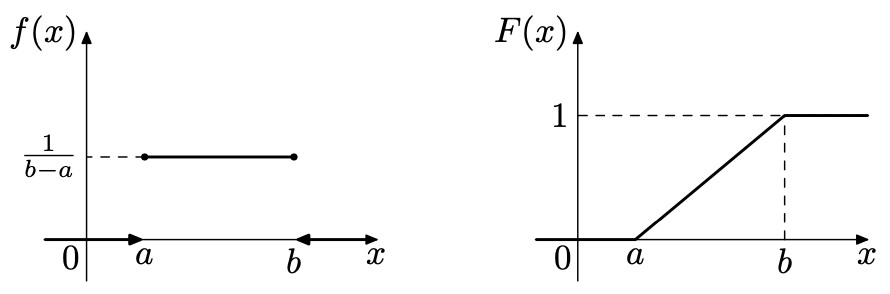
\includegraphics[width=0.01\textwidth]{pics/abs.png}
    % \caption{Пример равномерного распределения}
    % \label{abs}
% \end{figure}
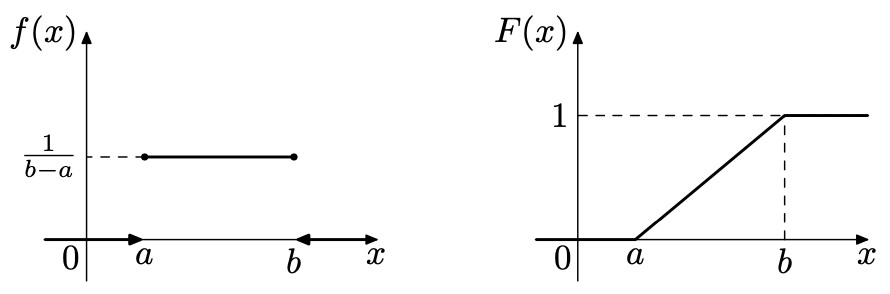
\includegraphics[width=\columnwidth]{pics/abs.png}


\textbf{Математическим ожиданием} случайной величины $\xi$ называется число $E\xi = \int\limits_{\Omega} \xi(\omega) P(d\omega)$ или $\int\limits_{-\infty}^{+\infty} x dF_{\xi}(x)$.
Если интеграл расходится, то говорят, что математического ожидания не существует.

В случае дискретной сл. вел.: $E\xi = \displaystyle\sum_{i} x_i p_i$.

В случае абсолютно непрерывной сл. вел.: $E\xi = \int x f(x) dx$

\textbf{Дисперсией} случайной величины $\xi$ называется число $D\xi = E(\xi - E\xi)^2$, $\sigma = \sqrt{D \xi}$ -- \textbf{среднеквадратическое отклонение}.

% Пусть $\xi$ и $\eta$ -- случайные величины. 
% Дисперсия их суммы в общем случае равна $D(\xi+n)=D \xi+D \eta + 2 \bigl( E (\xi \eta)-E \xi \, E \eta \bigr)$. 
Величина $\operatorname{cov}(\xi, \eta) \equiv E (\xi \eta)-E \xi \, E \eta$ называется \textbf{ковариацией} случайных величин $\xi$ и $\eta$. Если $\xi$ и $\eta$ независимы, то $\operatorname{cov}(\xi, \eta) = 0$. Обратное, вообще говоря, неверно.


\centerline{\textbf{Закон больших чисел в форме Чебышева}}

\textbf{Неравенство Чебышёва}
Если $\exists D\xi$, то $\forall \varepsilon > 0$
\begin{equation*}
    P(|\xi-E \xi| \geqslant \varepsilon) \leqslant \frac{D \xi}{\varepsilon^{2}}.
\end{equation*}


\begin{proof}
    Для $\varepsilon > 0$ неравенство $|\xi - E \xi| \geqslant \varepsilon \iff (\xi - E \xi)^2 \geqslant \varepsilon^2$, поэтому $P(|\xi-E \xi| \geqslant \varepsilon) = 
        P\left((\xi-E \xi)^{2} \geqslant \varepsilon^{2}\right) \leqslant 
        \cfrac{E (\xi-E \xi)^{2}}{\varepsilon^{2}} =
        \cfrac{D \xi}{\varepsilon^{2}}$.
\end{proof}

\textbf{Следствие}:
Если $\varepsilon = 3\sigma$, где $\sigma$ --- стандартное отклонение, то получим
\begin{equation*}
    P\bigl( |\xi-E \xi|> 3 \sigma \bigr) \leqslant 
    \frac{D \xi}{9 \sigma^2} = 
    \frac{D \xi}{9 \, D \xi} =
    \frac{1}{9} \iff 
    P\bigl( |\xi-E \xi| \leqslant 3 \sigma \bigr) \geqslant 
    1-\frac{1}{9} = 
    \frac{8}{9}.
\end{equation*}
Это соотношение называется \textbf{правилом трёх сигм}.

Последовательность случайных величин $\{\xi_n\}_{n = 1}^{+\infty}$ 
\textbf{сходится по вероятности} к случайной величине $\xi$ ($\xi_n \xrightarrow[]{\text{P}} \xi$), если
$$
    \forall \varepsilon>0 \quad P \biggl( \Bigl\{ \omega \colon |\xi_{n}(\omega)-\xi(\omega)|>\varepsilon \Bigr\} \biggr) \xrightarrow[n \to +\infty]{} 0.
$$

\textbf{Закон больших чисел в форме Чебышёва}:
$\forall$ последовательности $\xi_1, \xi_2, \ldots$ попарно независимых и одинаково распределённых случайных величин для которых $E \xi_i^2 < \infty \implies$ 
\begin{equation*}
    \frac{\xi_{1}+\ldots+\xi_{n}}{n} \xrightarrow[n \to + \infty]{\text{P}} E \xi_{1}.
\end{equation*}


\begin{proof}
    $S_n = \xi_1 + \ldots + \xi_n$, Из линейности матожидания получим
    \begin{equation*}
        E \left(\frac{S_{n}}{n}\right)=\frac{E \xi_{1}+\ldots+E \xi_{n}}{n}=\frac{n E \xi_{1}}{n}=E \xi_{1}.
    \end{equation*}
    
    Пусть $\varepsilon > 0$. Воспользуемся неравенством Чебышёва:
    \begin{multline*}
        P\left(\left|\frac{S_{n}}{n}-E \left(\frac{S_{n}}{n}\right)\right| \geqslant \varepsilon\right) \leqslant \frac{D\left(\frac{S_{n}}{n}\right)}{\varepsilon^{2}}
        = \frac{D S_{n}}{n^{2} \varepsilon^{2}}
        = \frac{D \xi_{1}+\ldots+D \xi_{n}}{n^{2} \varepsilon^{2}}= \\
        = \frac{n D \xi_{1}}{n^{2} \varepsilon^{2}}
        = \frac{D \xi_{1}}{n \varepsilon^{2}} \xrightarrow[n \to +\infty]{} 0,
    \end{multline*}
    т.к. $D\xi_1 < \infty$. Дисперсия суммы превратилась в сумму дисперсий в силу попарной независимости слагаемых, из-за которой все ковариации $\operatorname{cov}(\xi_i, \xi_j)$ по свойству ковариации обратились в нуль при $i \neq j$.
\end{proof}


\textbf{Центральная предельная теорема}:
    Пусть $\xi_{1}, \xi_{2}, \ldots$~--- последовательность независимых одинаково распределенных невырожденных случайных величин с $E \xi_{1}^{2}<\infty$ и $S_{n}=\xi_{1}+\ldots+\xi_{n}$. 
    Тогда
    \begin{equation*}
        P\left(\frac{S_{n}-E S_{n}}{\sqrt{D S_{n}}} \leqslant x\right)
        \xrightarrow[n \to +\infty]{}
        \Phi(x) = \frac{1}{\sqrt{2 \pi}} \int\limits_{-\infty}^{x} e^{-\frac{u^{2}}{2}} du~~ \forall x \in R
    \end{equation*}

\begin{proof}
Пусть $E \xi_{1}=m,\, D \xi_{1}=\sigma^{2}$. 
Введём $X = \xi_1 - m$ и $D \phi_X(t)=E e^{i tX}$ и 
$
    D \phi_{n}(t)=E e^{i t \frac{S_{n}-E S_{n}}{\sqrt{D S_{n}}}} = 
    \left[D \phi_X\left(\frac{t}{\sigma \sqrt{n}}\right)\right]^{n}
$

В силу разложения характеристической функции (при $\exists$ соответствующих моментов)
$
    D \phi_{X}(t)=1+i t E X+\ldots+\frac{(i t)^{n}}{n !} E X^{n}+R_{n}(t)
$

Т.к. $E X = E \left[ \xi_1 - m\right] = 0$, при $n=2$: 
$
    D \phi(t)=1-\frac{\sigma^{2} t^{2}}{2}+\overline{o}\left(t^{2}\right), \quad t \to 0
$.

$\forall t \in R$ при $n \to +\infty \implies $
$
    D \phi_{n}(t)=\left[1-\frac{\sigma^{2} t^{2}}{2 \sigma^{2} n}+\overline{o}\left(\frac{1}{n}\right)\right]^n \to e^{-\frac{t^{2}}{2}}
$

Функция $e^{-\frac{t^{2}}{2}}$ -- характеристическая функциия $N_{0,1}$. 
В силу теоремы о непрерывном соответствии между функциями распределения и характеристическими функциями Ц.П. теорема доказана.
\end{proof}

% -------- source --------
\bigbreak
[\cite[page 1-53]{stat_book}]
\vfill\null
\columnbreak
%---------------------3--------------------
\textbf{\LARGE osn 31. Методы Ньютона и секущих для решения нелинейных уравнений.}

% Рассматривается задача поиска корней нелинейного уравнения: нелинейные уравнения,
% вообще говоря, не имеют аналитического решения, поэтому для поиска решения
% используют вычислительные методы, хотя такое решение является лишь приближенным. Для конкретного итерационного метода необходимо специально выбирать
% начальное приближение, т.к. от этого выбора зависит сходимость рассматриваемых итерационных методов решения нелинейных уравнений.


\faEye \ ф-ию $f(x), ~x\in \mathbb{R}$, и ур-ие $f(x)=0.$

$\mathLet ~ x^* \in \mathbb{R}$~"--- корень уравнения, и определена его
окрестность радиуса $a$, не содержащая других корней уравнения: 
$U_a(x^*)=\{x:|x-x^*| < a\},$
причем заданная функция $f(x)$ определена на этой окрестности.
Считаем, что начальное приближение $x^0 \in U_a(x^*)$ задано.
Тогда для нахождения численного решения уравнения в
рассматриваемой окрестности необходимо построить последовательность
$\{x^n\}$, сходящуюся к~корню $x^*$ уравнения:
$\lim_{n\rightarrow\infty}f(x^n) = f(x^*) = 0.$
    
Численное решение нелинейных уравнений можно разбить на 2 этапа:
\begin{enumerate}
    \item Локализация корня, т.е. определение окрестности $U_a(x^*)$.
    \item Задание итерационного процесса~— построение последовательности
    $\{x^n\}$, сходящейся к~корню уравнения.
\end{enumerate}

\centerline{\textbf{Метод Ньютона}}

\mathLet \ в $U_a(x^*)$ существует и~не~обращается в~ноль непрерывная
первая производная функции $f(x)$: $f'(x) \neq 0,~~~x\in U_a(x^*).$

Разложим $f(x^*)$ по~формуле Тейлора в~малой окрестности точки $x\in U_a(x^*)$:
$f(x^*) =  f(x) + (x^* - x)f'(x) + \dots$, 
и отбросим в этом разложении величины, имеющие второй и выше порядок малости
по $(x^* - x)$.

Заменив $x^*$ на $x^{n+1}$ и $x$ на $x^n$, получим ур-ие 
$ f(x^n) + (x^{n + 1} - x^n)f'(x^n) = 0,~~~n\in \mathbb{Z}_+.$

Учитывая, что $f'(x^n) \neq 0$, имеем:
%
    \begin{equation}
    %
        \label{iter_proc}
        %
        x^{n + 1} = x^n - \frac{f(x^n)}{f'(x^n)},~~~n \in \mathbb{Z}_+.
    %
    \end{equation}
    %
%
Итерационный процесс поиска корня уравнения $f(x)=0$, задаваемый формулой \eqref{iter_proc},
наз-ся \textbf{итерационным методом Ньютона}.

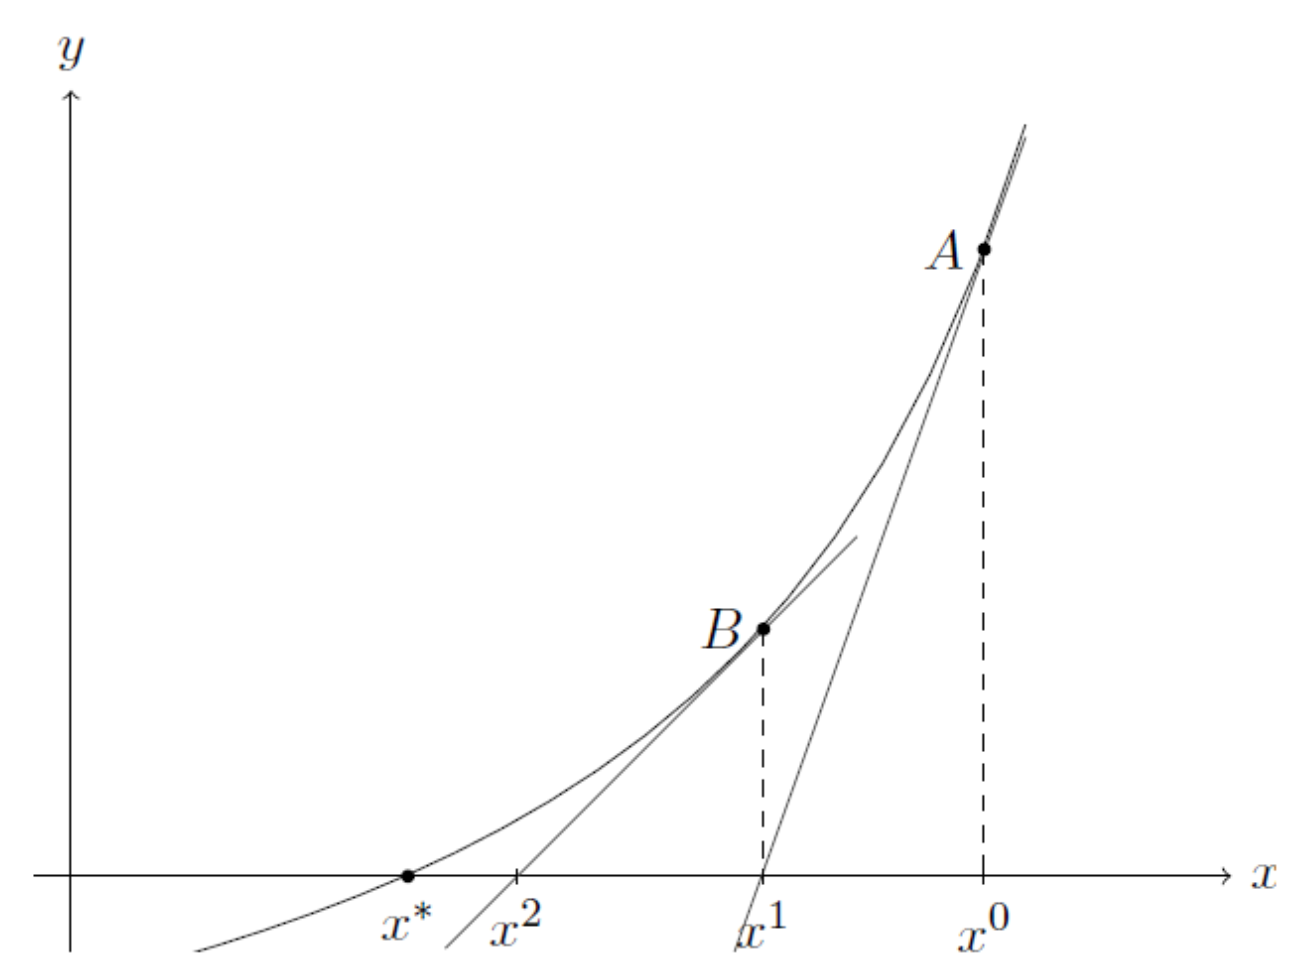
\includegraphics[scale=0.4]{pics/osn_30_0.png}

% \begin{figure}[h!]
%     \centering
%     \includegraphics[width=0.1\textwidth]{}
%     \caption{Геометрическая интерпретация метода Ньютона}
%     \label{fig:newton}
% \end{figure}
\faEye \ т. $A(x^0,f(x^0))$. Определим первую итерацию $x^1$ как абсциссу точки пересечения с осью $Ox$ касательной к $f(x)$, проведенной через т. $A$. Аналогично получаем значение $x^2$. Продолжая, на $n$-ом шаге получим значение $x^n$, приближающее корень $x^*$ уравнения $f(x)=0$ с заданной точностью.

\textbf{Зам.} При решении задач на практике часто рассматривается модифицированный
метод Ньютона, задаваемый формулой $ x^{n + 1} = x^n - \frac{f(x^n)}{f'(x^0)},~~n\in\mathbb{Z_+}$ (чтобы считать пр-ую только один раз).

\centerline{\textbf{Метод секущих}}

В методе Ньютона (\ref{iter_proc}) заменим $f'(x)$ на его дискретный аналог $\frac{f(x^n)-f(x^{n-1})}{x^n-x^{n-1}}$, получаем итерационный метод:
\begin{equation}
    x^{n+1} = x^n - \frac{(x^n - x^{n-1})f(x^n)}{f(x^n) - f(x^{n-1})}
    \label{sec}
\end{equation}
  
Итерационный процесс \ref{sec} задает двухшаговый метод решения уравнений, называемый \textbf{методом секущих}.

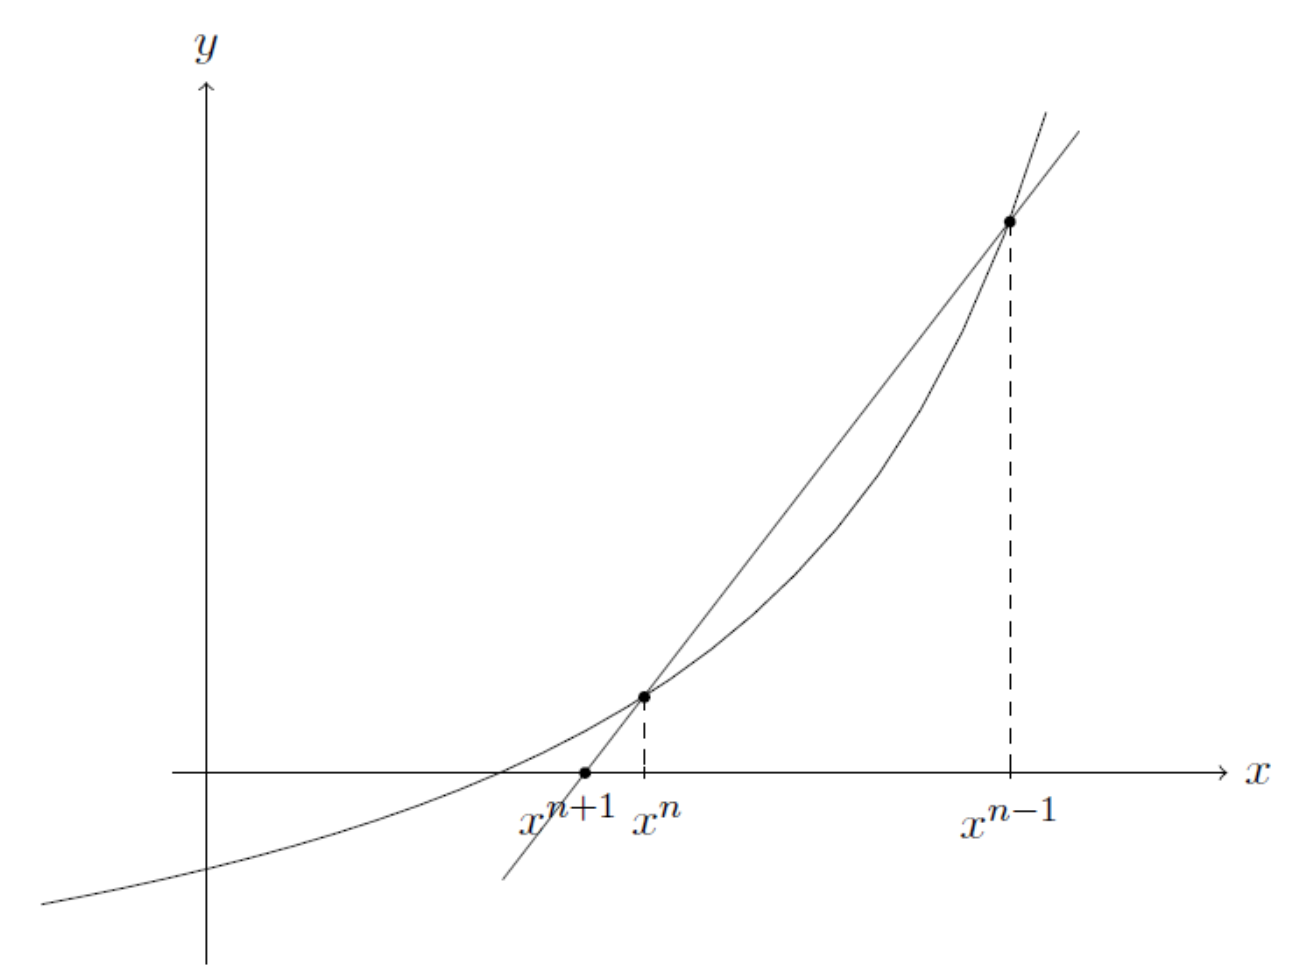
\includegraphics[scale=0.4]{pics/osn_30_1.png}

\centerline{\textbf{Сходимость метода Ньютона}}

Если рассмотреть итерационный метод Ньютона как метод простой итерации ($x^{n+1}=S(x^n), n\in \mathbb{Z_+}$) 
с функцией $S(x) = x - \frac{f(x)}{f'(x)}.$

$|S'(x)| < 1$ при $x \in U_a(x^*)$, то он сходится.
Предполагая, что функция $f(x)$ дифференцируема достаточное число раз,
продифференцируем функцию $S(x)$:
%
$$
    S'(x) = 1 - \frac{(f'(x))^2 - f(x)f''(x)}{(f'(x))^2} =
    \frac{f(x)f''(x)}{(f'(x))^2}.
$$%

\textbf{Теорема}: $\mathLet ~ \exists$ такая константа $M > 0$, для которой выполнена оценка
$\frac{1}{2}\left|S''(x)\right| \leqslant M, ~~~x \in U_a(x^*).$ 
Тогда если начальное приближение $x^0$ выбрать в соответствии с условием
$ |x^0 - x^*| < \frac{1}{M},$
то итерационный метод Ньютона сходится, и имеет место оценка:
$ |x^n - x^*| \leqslant \frac{1}{M}\left(M|x^0 - x^*|\right)^{2^n}.$

\begin{proof} Погрешность приближенного решения: $z^n = x^n - x^*.$
% Покажем, что связь между $z^n$ и $z^{n+1}$ квадратичная.

\faEye \ выражение для $z^{n+1}$:
$z^{n + 1} = x^{n + 1} - x^* = S(z^n + x^*) - S(x^*).$

Разложим $S(z^n + x^*)$ по формуле Тейлора и учитывая $S'(x^*)=0$:

$$
    z^{n + 1} = S(x^*) + S'(x^*)z^n +
    \frac{1}{2}S''(\tilde{x}^n)\left(z^n\right)^2 - S(x^*) =
    \frac{1}{2}S''(\tilde{x}^n)(z^n)^2,
$$

$$
    ~~~\tilde{x}^n=x^n+\theta z^n, ~\theta\in\mathbb{R}, ~|\theta|<1.
$$

\mathLet \ функция $f(x)$ трижды непрерывно дифференцируема в окрестности
$U_a(x^*)$. Тогда $S''(x) = \left(\frac{f(x)f''(x)}{(f'(x))^2}\right)'.$
    

$\mathLet ~ \exists$ постоянная $M > 0$ такая, что для любого $x \in U_a(x^*)$
выполняется неравенство $M \geqslant \frac{1}{2}\left|S''(x)\right|.$

Из этого неравенства и уравнения $z^{n + 1}$ следует оценка
$|z^{n+1}| \leqslant M|(z^n)^2|.$

Домножим это неравенство на $M$ и обозначим $v^n = M|z^n|$.
Тогда получим, что $v^{n+1} \leqslant (v^n)^2.$

Отсюда следует, что $v^n \leqslant (v^0)^{2^n}$, значит,
$ M|z^n| \leqslant \left(M\left|z^0\right|\right)^{2^n},$
$ |z^n| \leqslant \frac{1}{M} \left(M\left|z^0\right|\right)^{2^n}.$

Введем обозначение $q = M|z_0|$. Если $0< q < 1$,
то последовательность $\{z^n\}_{n=0}^\infty$ стремится к нулю:
$z^n \underset{n\rightarrow\infty}\longrightarrow 0,$
и итерационный метод Ньютона сходится. Условие на $q~(0<q<1)$ будет выполнено,
если $0<|z^0|<\frac{1}{M}$, то есть $|x^0 - x^*| < \frac{1}{M}$. \end{proof}

% -------- source --------
\bigbreak
[\cite[page 99-107]{chimi}]
\vfill\null
\columnbreak
%---------------------
\end{multicols}
\end{tcolorbox}
% --- END OF PAGE ----



% --- BEGIN OF PAGE ----
\newpage
\begin{tcolorbox}[colback=white, left=0mm, right=0mm]
\begin{multicols}{4}
%---------------------0--------------------
\textbf{\LARGE osn 32. Численное решение задачи Коши для обыкновенных дифференциальных уравнений. Примеры методов Рунге-Кутта.}

% Пишет Дима

Рассматривается задача Коши для системы ОДУ:
\begin{equation}
%
    \label{Koshi_sys}
    %
    \begin{cases}
    %
        \dfrac{du}{dt} = f(t, u(t)), \quad t > 0, \\
        u(0) = u_0,
    %
    \end{cases}
    %
\end{equation}
%
где
$u(t)=\left(u_1(t), \dots, u_m(t)\right)^T$, $f(t, u(t)) = \left(f_1(t, u(t)), \dots, f_m(t,u(t)\right)^T$.

Обозначим $ | u(t) | = \sqrt{u_1^2(t) + u_2^2(t) + \ldots + u_m^2(t)}$.

\textbf{Теорема}: Пусть $f(t, u(t))$ непрерывна в параллелепипеде 
$ R = \{|t| \leqslant a, | u(t)-u(0)| \leqslant b,\; a, b\in\mathbb{R}\} $ 
и уд-ет в $R$ условию Липшица по второму аргументу, т.е. 
$|f(t, u) - f(t, v)| \leqslant L|u - v|$
, для всех $(t, u)$, $(t, v) \in R$\\ 
$\implies $
$\exists!$ решение $u(t)$ задачи \eqref{Koshi_sys}, определенное и непрерывное на некотором отрезке.


% В настоящее время наибольшее распространение получили две группы численных
% методов решения задачи Коши:
% %
% \begin{enumerate}
%     \item Методы Рунге--Кутта;
%     \item Многошаговые разностные методы, наиболее известными из которых являются
%         методы Адамса.
% \end{enumerate}

В приведенных ниже примерах для простоты изложения предполагается, что
система \eqref{Koshi_sys} состоит всего из одного уравнения.

\centerline{\textbf{Нахождение численного решения}}


Для нахождения численного решения вводится сетка по времени с постоянным шагом $\tau>0$, т.е. множество точек
$\omega_\tau = \{t_n = n\tau,\;n \in \mathbb{Z}_+\}$, и обозначим
$u_n = u(t_n)$, $f_n = f(t_n, u_n)$.
Точное решение задачи \eqref{Koshi_sys} будем обозначать буквой $u$,
а \textbf{приближенное решение} (сеточная ф-ия) --- буквой $y$: $y_n = y_n(t_n)$.

\todo{ про численное решение }

\bigbreak

\centerline{\textbf{Двухэтапный метод Рунге--Кутта}}
Общий вид двухэтапного метода Рунге--Кутта для уравнения \eqref{Koshi_sys}:
\begin{equation}
%
    \label{Runge-Kutt}
    %
    \begin{cases}
    %
        \dfrac{y_{n+1} - y_n}{\tau} = \sigma_1 K_1 + \sigma_2 K_2,~~~n\in \mathbb{Z}_+ \\
        y_0 = u_0, \\
        K_1 = f(t_n, y_n), \quad K_2 = f(t_n + a_2\tau, ~ y_n + b_{21} \tau f(t_n, y_n)),
    %
    \end{cases}
    %
%
\end{equation}
где $\sigma_1, \sigma_2,a_{2}, b_{21} \in\mathbb{R}$~"--- некоторые числа, от выбора которых зависит как погрешность аппроксимации, так и точность численного решения.

Подставим значения $K_1$ и $K_2$ в первое уравнение системы \eqref{Runge-Kutt}:
%
$$
    \frac{y_{n+1} - y_n}{\tau} = \sigma_1 f(t_n, y_n) +
    \sigma_2 f(t_n + a_2 \tau, y_n + b_{21} \tau f(t_n, y_n)).
$$
%
Рассмотрим \textbf{погрешность аппроксимации} разностной схемы \eqref{Runge-Kutt}
на решении задачи \eqref{Koshi_sys}:
%
\begin{equation}
%
    \label{Runge-Kutt_appr}
    %
    \psi_n = - \frac{u_{n+1} - u_n}{\tau} + \sigma_1 f(t_n, u_n) +
    \sigma_2 f\left(t_n+a_2\tau, u_n + b_{21}\tau f(t_n, u_n)\right).
%
\end{equation}

\textbf{Утв.}: Погрешность аппроксимации этого метода имеет второй порядок малости по $\tau$: $\psi_n = O(\tau^2)$ при $\sigma_2 = \sigma, \sigma_1 = 1-\sigma, a_2 = b_{21} = \sigma/2$.

\begin{proof}

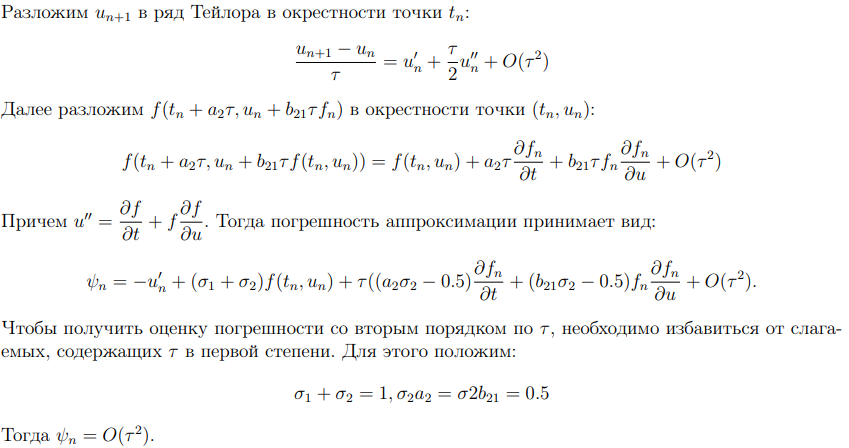
\includegraphics[scale=0.4]{pics/osn_31_new.png}

\end{proof}

\textbf{Погрешность решения} разностной схемы~\eqref{Runge-Kutt}: $z_n = y_n - u_n,  n\in\mathbb{Z}.$

\textbf{Утв.}: Общий двухэтапный метод Рунге--Кутта
при выполнении соответствующих условий
имеет квадратичную точность по $\tau$, т.е. при достаточно малых $\tau$: $|z_{n+1}| = O(\tau^2)$, совпадающую с оценкой погрешности аппроксимации на решении исходного уравнения \eqref{Koshi_sys}

Частные случаи общего двухэтапного метода Рунге--Кутта:

\begin{enumerate}
%
    \item При $\sigma=1,~~a=a_2=0.5,~~b=b_{21}=0.5$ мы получим схему Рунге--Кутта <<предиктор--корректор>>:
    $y_{n+1} = y_n + \tau f(t_{n+\frac12}, y_n + 0.5\tau f(t_n, y_n)).$
    Погрешность этой схемы равна $O(\tau^2)$.

    \item Если положить $\sigma=0.5,~~a=1,~~b=1$, то мы получим симметричную разностную схему:
    %
    $$\dfrac{y_{n+1} - y_n}{\tau} = 0.5 \left(f(t_n, y_n) +
      f(t_n + \tau, y_n + \tau f_n)\right), n\in\mathbb{Z}_+, y_0 = u_0.
    $$
    %
    Эта разностная схема является очень эффективной, имеет второй
    порядок точности по $\tau$ и часто используется на практике.
    %
\end{enumerate}




\centerline{\textbf{Общий $m$-этапный метод Рунге--Кутта}}

Общая идея $m$-этапного метода Рунге--Кутта заключается в том, что
для вычисления значения приближенного решения в каждой следующей точке $t_{n+1}$
вводятся $m$ дополнительных этапов.
Промежуточные значения на каждом шаге $n\in\mathbb{Z}_+$ вычисляются по формулам:
$$
\begin{aligned}
%
    &K_1 = f(t_n, y_n), \\
    &K_2 = f(t_n + a_2\tau, y_n + b_{21} \tau K_1), \\
    &K_3 = f(t_n + a_3\tau, y_n + b_{31}\tau K_1 + b_{32}\tau K_2), \\
    &\dots \\
    &K_m = f(t_n+a_m\tau, y_n + b_{m1} \tau K_1 + b_{m2} \tau K_2 + \ldots + b_{m m -1} \tau K_{m-1}).
%
\end{aligned}
$$
%
При этом разностная схема для исходной задачи~\eqref{Koshi_sys}
имеет вид
%
\begin{equation}
    %
    \label{gen_Runge-Kutt_meth}
    %
    \begin{cases}
        \dfrac{y_{n+1} - y_n}{\tau} = \sigma_1 K_1 + \sigma_2 K_2 + \ldots + \sigma_m K_m \\
        y_0 = u_0, n \in \mathbb{Z}_+,
    \end{cases}
    %
\end{equation}
%
где $\sigma_1, \ldots, \sigma_m \in\mathbb{R}$, и выполнено условие аппроксимации: $\sum\limits_{i=1}^{m} \sigma_i = 1.$

Примеры трех- и четырех- этапных методов Рунге--Кутта, имеющих третий и четвертый порядок точности соответственно:
%

\begin{enumerate}
%
    \item \textbf{$m=3$}: $\dfrac{y_{n+1} - y_n}{\tau} = \frac16(K_1 + 4K_2 + K_3),$ где
    %
    $$
        \begin{aligned}
            &K_1 = f(t_n, y_n), \\
            &K_2 = f(t_n + 0.5 \tau, y_n + 0.5 \tau K_1), \\
            &K_3 = f(t_n + \tau, y_n - \tau K_1 + 2\tau K_2).
        \end{aligned}
    $$
    Данная схема имеет третий порядок точности по $\tau$: $O(\tau^3)$.

    \item \textbf{$m=4$}: $\dfrac{y_{n+1} - y_n}{\tau} = \frac16 (K_1 + 2K_2 + 2K_3 + K_4),$ где
    
    $$
        \begin{aligned}
            &K_1 = f(t_n, y_n), \\
            &K_2 = f(t_n+0.5\tau, y_n + 0.5\tau K_1), \\
            &K_3 = f(t_n + 0.5 \tau, y_n + 0.5 \tau K_2), \\
            &K_4 = f(t_n + \tau, y_n + \tau K_3).
        \end{aligned}
    $$
    Данная схема имеет четвертый порядок точности по $\tau$: $O(\tau^4)$.

\end{enumerate}

%
\textbf{Замечание}: Формулы $m$-этапного метода Рунге--Кутта достаточно громоздки. Это является одной из причин того, что на практике редко используются методы Рунге--Кутта для $m > 4$.
%




% -------- source --------
\bigbreak
[\cite[page 152-163]{chimi}]
\vfill\null
\columnbreak
%---------------------1--------------------
\textbf{\LARGE osn 30. Квадратурные формулы прямоугольников, трапеций и парабол.}

\textbf{Задача:} Вычислить определенный интеграл $I = \int\limits_a^b f(x)dx$.

Не всегда можно посчитать аналитически, но есть универсальные алгоритмы -- формулы численного интегрирования (квадратурные формулы). 
В них интеграл заменяется конечной суммой:

$ \int\limits_a^b f(x)dx \approx\displaystyle\sum_{k=0}^N C_k f(x_k)$ --- \textbf{квадратурная формула}, 
$C_k$ --- \textbf{коэффициенты квадратурной формулы}, 
$x_k \in [a, b]$ --- \textbf{узлы квадратурной формулы}.

$\psi = \int\limits_a^b f(x)dx - \sum_{k=0}^N C_k f(x_k) $ --- \textbf{погрешность квадратурной формулы}. 

Введем на $[a,b]$ равномерную сетку $\omega_n = \{x_i =a+ih,~i\in[0,N],~N_h=b-a \}$.

$\int\limits_a^b f(x)dx = \displaystyle\sum_{i=0}^N\int\limits_{x_{i-1}}^{x_i} f(x)dx$. Строим квадратурные формулы для $\int\limits_{x_{i-1}}^{x_i} f(x)dx$.

\textbf{Формула прямоугольников.}

$$ \int\limits_{x_{i-1}}^{x_i} f(x)dx \sim f \left( x_{i-\frac{1}{2}} \right) h $$

$\psi_i = \int\limits_{x_{i-1}}^{x_i} f(x)dx - f \left( x_{i-\frac{1}{2}} \right)h = 
\int\limits_{x_{i-1}}^{x_i} \left( f(x) - f\left(x_{i-\frac{1}{2}} \right) \right)dx = 
\int\limits_{x_{i-1}}^{x_i} 
\Biggl( 
    f(x_{i-\frac{1}{2}}) + 
    (x - x_{i-\frac{1}{2}})f'(x_{i-\frac{1}{2}}) + 
    \frac{\left(x - x_{i-\frac{1}{2}}\right)^2}{2}f''(\xi) 
    \Biggr|_{\xi \in [x_{i-1};x_i]} - 
    f(x_{i-\frac{1}{2}}) 
\Biggr) dx$

$|\psi_i| \leqslant 
M_{2i} \int\limits_{x_{i-1}}^{x_i} \frac{ \left(x - x_{i-\frac{1}{2}} \right)^2}{2}dx = 
\frac{h^3}{24} M_{2i}$, где $ M_{2i} = \displaystyle\max_{x\in[x_{i-1};x_i]}|f''(x)|$

$\int\limits_a^b f(x)dx \sim \displaystyle\sum_{i=0}^N f(x_{i-\frac{1}{2}})h$

$\psi = \displaystyle\sum_{i=0}^N \psi_i \leqslant \displaystyle\sum_{i=0}^n \frac{h^3}{24} M_{2i}\leqslant \frac{M_2Nh^3}{24} = \frac{M_2h^2(b-a)}{24} \implies \psi = O(h^2)$

\textbf{Формула трапеций.}

$$ \int\limits_{x_{i-1}}^{x_i} f(x)dx \sim \frac{f(x_{i-1}) +f (x_i)}{2}h $$
получается путем замены $f(x)$ интерполяционным многочленом первой степени, построенным по узлам $x_{i-1},~x_i$.

$$L_{1i} = \frac{\left((x-x_{i-1})f(x_i)-(x-x_i)f(x_{i-1})\right)}{h}$$

$$f(x) - L_{1i} = \frac{( x-x_{i-1})(x-x_i )}{2}f''(\xi_i(x))$$

$\left|\psi_j\right| =  \int\limits_{x_{i-1}}^{x_i} f(x)dx - \frac{f(x_{i-1}) +f (x_i)}{2}h = \int\limits_{x_{i-1}}^{x_i} (f(x) - L_{1i})dx =$ \\
$= \int\limits_{x_{i-1}}^{x_i} \frac{(x-x_{i-1})(x-x_i)}{2}f''(\xi_i(x)) \implies |\psi_j| \leqslant \frac{M_{3j}h^3}{12}$

$ \int\limits_a^b f(x)dx \sim \displaystyle\sum_{i=1}^N\frac{f(x_{i-1}) +f (x_i)}{2}h = $

$ = h \left(0.5f(x_0) + f(x_1) + f (x_2) + \dots + f(x_{N-1}) + 0.5f(x_N ) \right)$
--- составная формула трапеций. 

$$|\psi| \leqslant \frac{M_3h^2(b-a)}{12} = O(h^2)$$

\textbf{Формула Симпсона (парабол).}

$L_n = \displaystyle\sum_{k=0}^n L_{n_k} = \displaystyle\sum_{k=0}^n \frac{\omega(x)}{(x-x_k)\omega'(x_k)}f(x_k)$
--- интерполяционный полином в Форме Лагранжа, где

$$\omega(x) = \displaystyle\prod_{j=0}^n(x-x_j),~\omega'(x_k)=\displaystyle\prod_{\substack{j=0 \\ j\neq k}}^n (x_k - x_j),~f(x) - L_n = \frac{f^{(n+1)}(\xi(x))}{(n+1)!}\omega(x)$$

В формуле Симпсона:

$f(x) \sim L_2 \sim \frac{(x-x_{i-\frac{1}{2}})(x-x_i)}{(x_{i-1}-x_{i-\frac{1}{2}})(x_{i-1}-x_i)}f(x_{i-1}) + \frac{(x-x_{i-1})(x-x_i)}{(x_{i-\frac{1}{2}}-x_{i-1})(x_{i-\frac{1}{2}}-x_{i-1})}f(x_{i-\frac{1}{2}}) + \frac{(x-x_{i-1})(x-x_{i-\frac{1}{2}})}{(x_i-x_{i-1})(x_i-x_{i-\frac{1}{2}})}f(x_{i}) = \frac{2}{h^2}((x-x_{i-\frac{1}{2}})(x-x_i)f(x_{i-1})-2(x-x_{i-1})(x-x_i)f(x_{i-\frac{1}{2}}) + (x-x_{i-1})(x-x_{i-\frac{1}{2}})f(x_i)),~ \forall x\in[x_{i-1},x_i]$

$$\int\limits_{x_{i-1}}^{x_i} L_{2_i}(x) dx = \frac{h}{6}(f(x_{i-1}) + 4f(x_{i-\frac{1}{2}}) + f(x_i)) $$
$$\implies \int\limits_{a}^{b} f(x) dx \approx \displaystyle\sum_{i=1}^{N}\frac{h}{6}(f(x_{i-1}) + 4f(x_{i-\frac{1}{2}}) + f(x_i))$$
$$\int\limits_{a}^{b} L_{2}(x) dx \approx \frac{h}{6}(f_0 + f_N + 2(f_1 + \dots + f_{N-1}) + 4(f_{\frac{1}{2}} + \dots + f_{N - \frac{1}{2}})) $$

$$ \psi_i \leqslant \frac{M_{4i}h^4}{2880},~|\psi| \leqslant \frac{M_4h^4(b-a)}{2880} \implies \psi = O(h^4)$$

\todo{сюда бы картинки разбиенитя площади под кривой для разных методов}

% -------- source --------

\vfill\null
\columnbreak
%---------------------2--------------------
\textbf{\LARGE osn 28. Схемы из функциональных элементов и простейшие алгоритмы их синтеза. Оценка сложности схем, получаемых по методу Шеннона.}

\textbf{Орграф} -- это ориентированный граф.

Вершины орграфа, в которые не входит ни одной дуги, называются \textbf{истоками}.

Орграф называется \textbf{ациклическим}, если в нем нет ориентированных циклов.

Систему Б = {$g_1$, $g_2$, ..., $g_m$}, где все $g_i$ — функции алгебры логики, будем называть \textbf{базисом функциональных элементов}.

Орграф называется \textbf{упорядоченным}, если для каждой вершины $v_i$, в которую входит $k_i$ дуг, задан порядок $e_1$, $e_2$, ..., $e_{k_i}$ этих дуг.

\bigbreak

\textbf{Схемой из функциональных элементов} в базисе Б называется ациклический упорядоченный орграф, в котором:
\begin{itemize}
    \item каждому истоку приписана некоторая переменная, причем разным истокам приписаны разные переменные (истоки при этом называются входами схемы, а приписанные им переменные — входными переменными);
    \item каждой вершине, в которую входят k $\geq$ 1 дуг, приписана функция из базиса Б, зависящая от k переменных(вершина с приписанной функцией при этом называется \textbf{функциональным элементом}); 
    \item некоторые вершины выделены как \textbf{выходы}. 
\end{itemize}

\textbf{Сложностью} схемы из функциональных элементов называется число функциональных элементов в схеме (число внутренних вершин).

Пример:

\textbf{Полусумматор} Пусть $v$ и $v_1$ — выходы на рисунке, $f_v$ = x$\wedge$y $\wedge$ (x $\vee$ y)= x + y ; $f_{v_1}$ = x$\wedge$y . Сложность (число элементов) полусумматора равна 4.

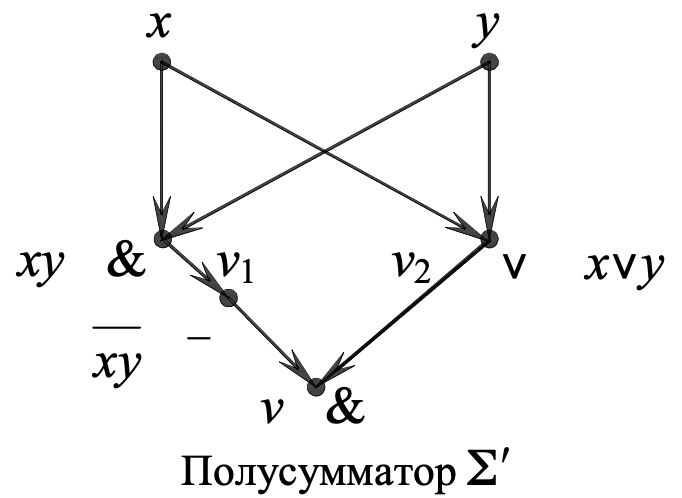
\includegraphics[width=0.5\columnwidth]{pics/pol_sum.png}

% \textbf{Сумматором $S_n$} порядка n называется схема с 2n входами $x_1$, $x_2$, ..., $x_n$, $y_1$, $y_2$, ..., $y_n$ и n + 1 выходом $z_0$, $z_1$, $z_2$, ..., $z_n$ такая, что |$\widetilde{z}$| = |$S_n$ ($\widetilde{x}$,$\widetilde{y}$)| = |$\widetilde{x}$| + |$\widetilde{y}$|.

% \textbf{Теорема} Существует схемный сумматор порядка n в базисе \{$\wedge$, $\vee$, $\bar{}$ \} с числом элементов 9n – 5.

% 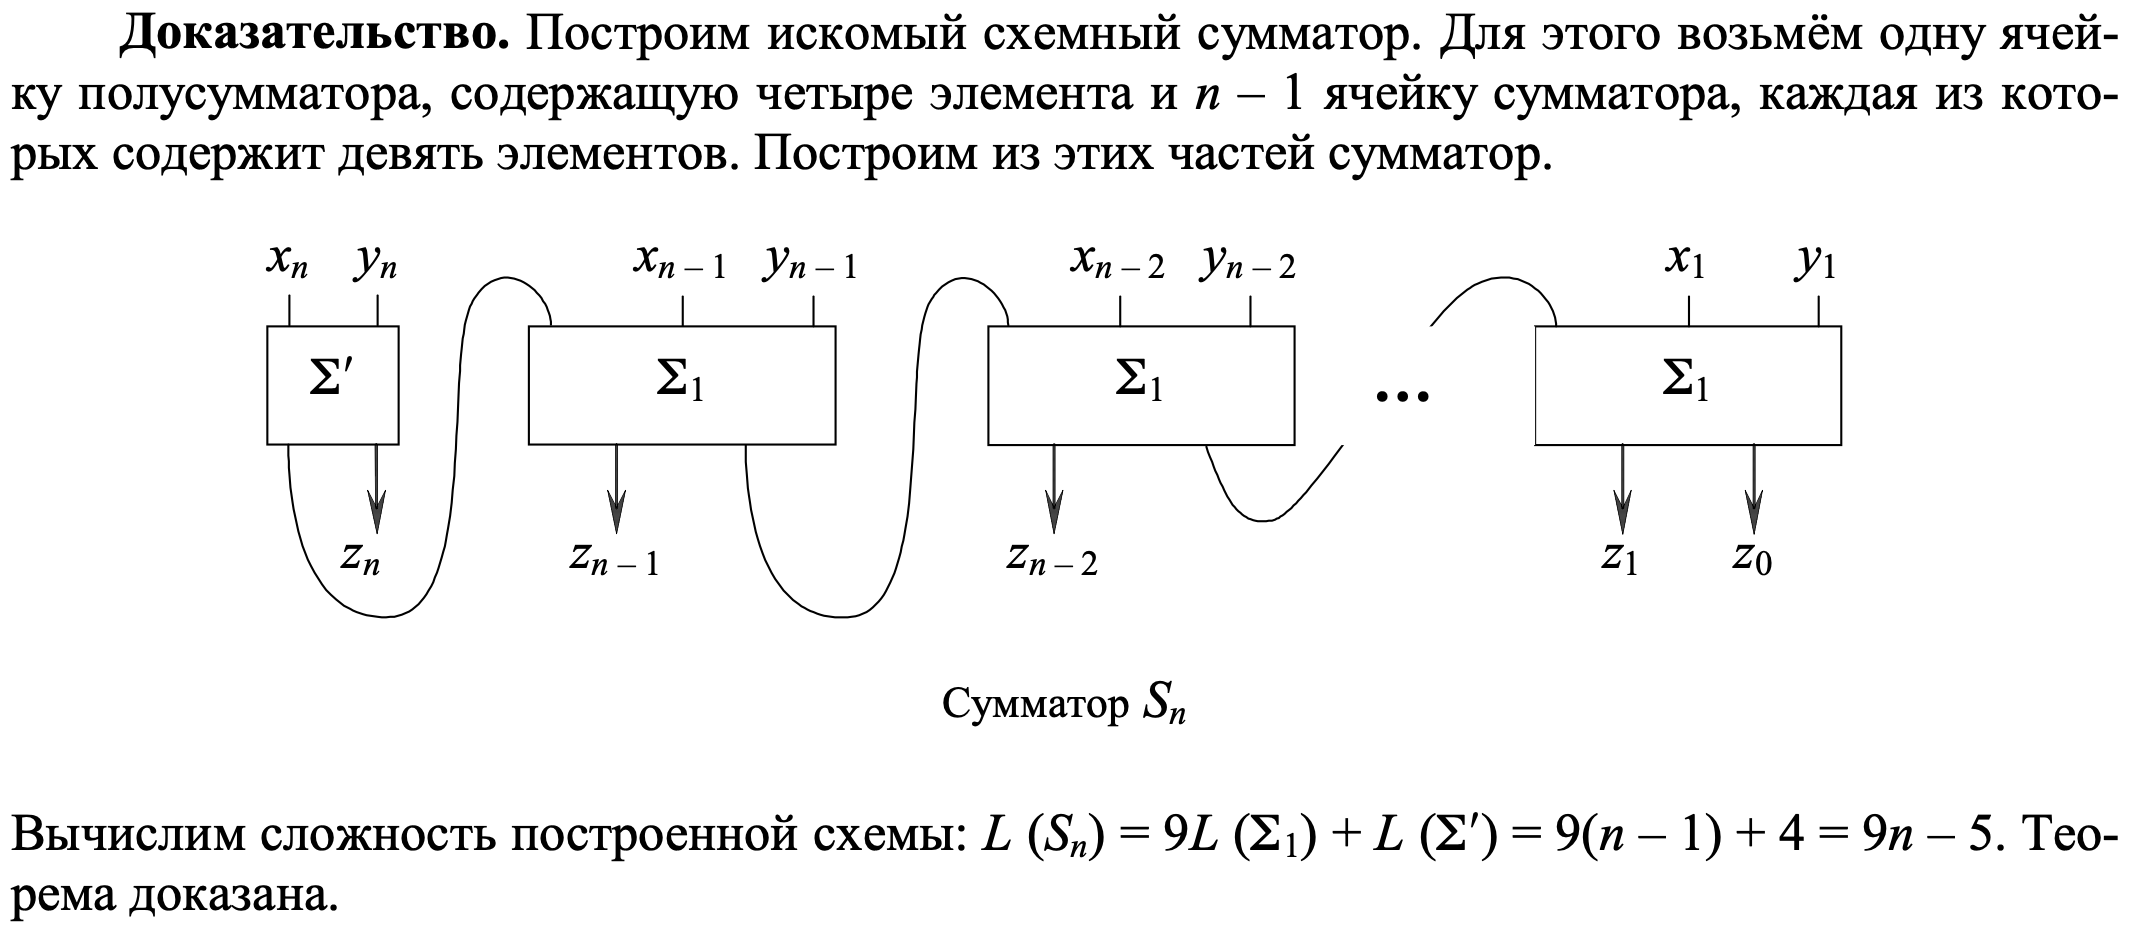
\includegraphics[width=\columnwidth]{pics/sum.png}

% \textbf{Вычитателем $W_n$} порядка n называется схема с 2n входами $x_1$, $x_2$, ..., $x_n$,
% $y_1$, $y_2$, ..., $y_n$ и n выходами $z_1$, $z_2$, ..., $z_n$ такая, что при |x| $\geq$ |y|, |$\widetilde{z}$| = |W ($\widetilde{x}$,$\widetilde{y}$)| = |$\widetilde{x}$| - |$\widetilde{y}$|.

% \textbf{Теорема} Существует схемный вычитатель порядка n в базисе \{$\wedge$, $\vee$, $\bar{}$ \} с числом элементов 9n – 5.

% 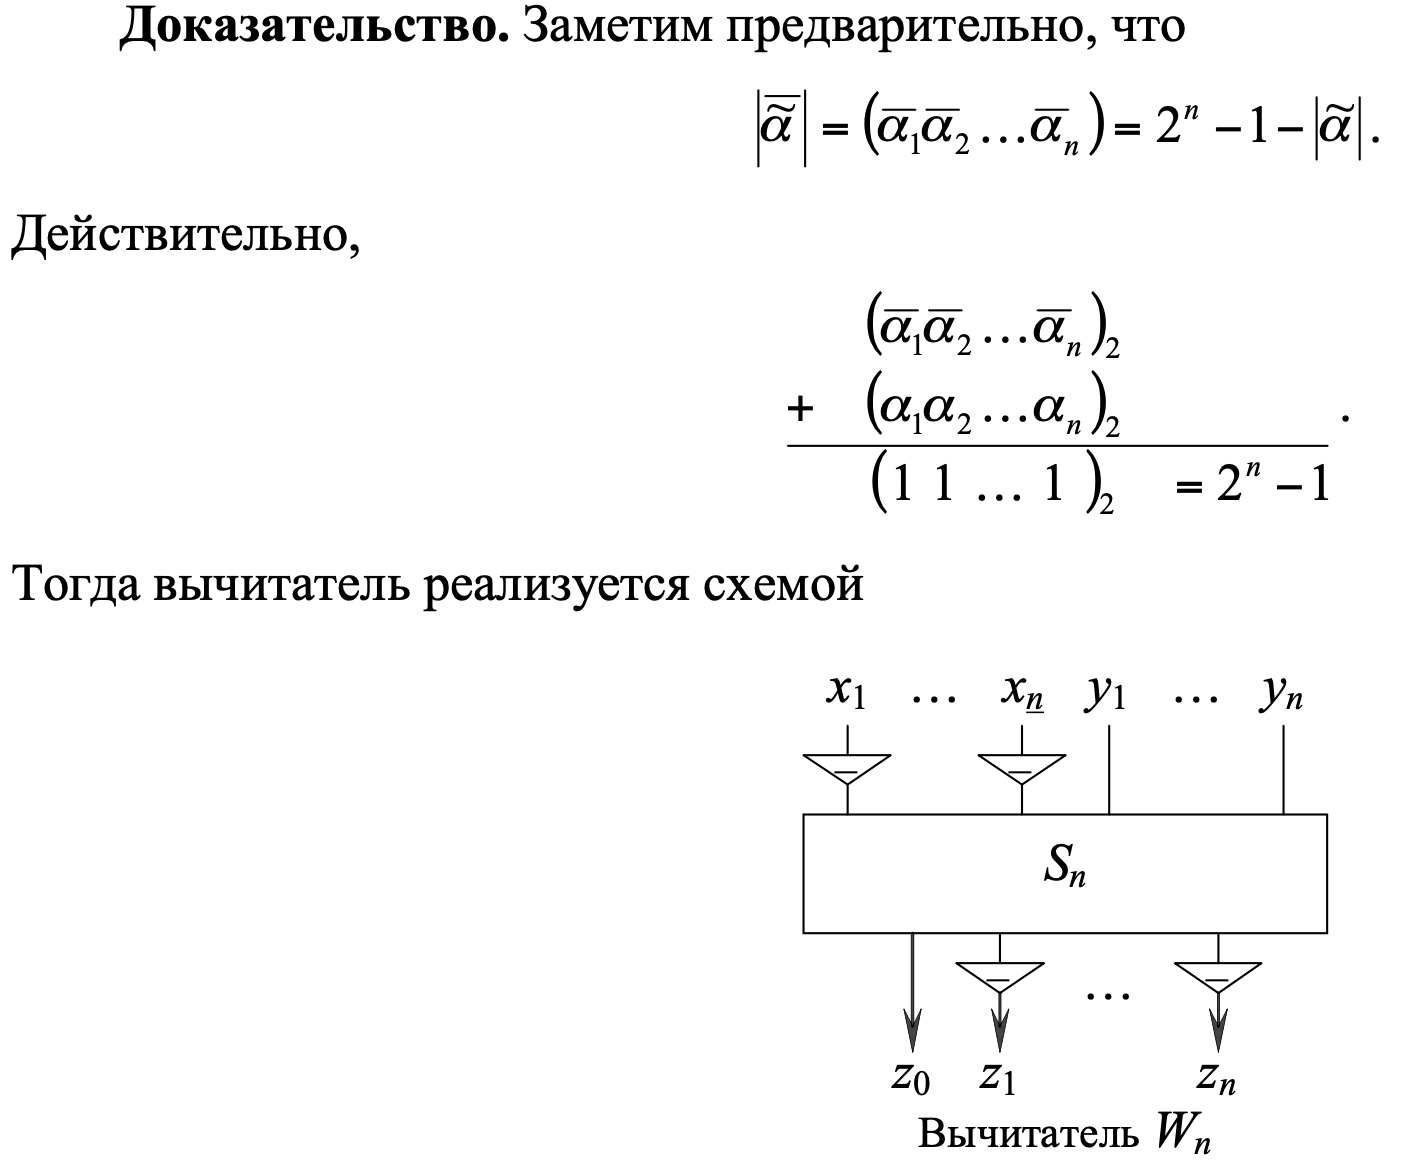
\includegraphics[width=\columnwidth]{pics/wich.png}

% |$W_n$ ($\widetilde{x}$,$\widetilde{y}$)| = |$\widetilde{x}$| - |$\widetilde{y}$| = $2_n$ - 1 - (($2_n$ - 1 - |$\widetilde{x}$|) + |$\widetilde{y}$|)
% и его можно построить, используя 2n отрицаний и 1 сумматор порядка n. При этом L ($W_n$) = 2n + L ($S_n$) = 2n + (9n – 5) = 11n – 5. Поскольку $\widetilde{x}$ $\geq$ $\widetilde{y}$, то ($2_n$ - 1 - |$\widetilde{x}$|) + |$\widetilde{y}$| $\leq$ $2_n$ - 1, и выход вычитателя определен. Теорема доказана.

% \bigbreak

% \textbf{Метод Шеннона.}
    
% Выбираем параметр $q$, $1 \leqslant q \leqslant n$.

% Используется \textbf{разложение Шеннона}:
% $$ f(\underbrace{x_1,\dots,x_q}_{x'},\underbrace{x_{q+1},\dots,x_n}_{x''}) = $$
% $$ = \displaystyle\bigvee_{\sigma''=(\sigma_{q+1},\dots,\sigma_n)} x_{q+1}^{\sigma_{q+1}}\cdots x_n^{\sigma_n}\cdot f_{\sigma''}(x_1,\dots,x_q,\sigma_{q+1},\dots,\sigma_n)$$

% Для любой ФАЛ $f \in P_2(n)$ строим СФЭ $\Sigma_f$ как суперпозицию $\Sigma''(\Sigma')$, где $\Sigma''$ --- мультиплексор, $\Sigma'$ --- универсальный многополюсник.

% 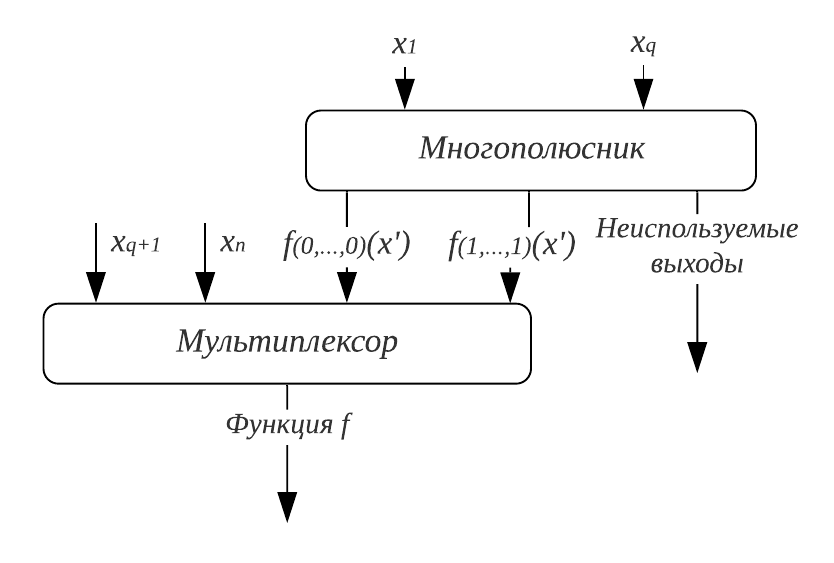
\includegraphics[width=\columnwidth]{pics/osn27_oki.png}
% Схема для $\Sigma_f = \Sigma''(\Sigma')$


% Сложность многополюсника от $q$ переменных: $L(\Sigma') \leqslant 2^{2^q} - q $ (следует из леммы)

% Сложность мультиплексора от $n-q$ переменных: $L(\Sigma'') \leqslant 2^{n - q + 2} - 3$

% Полагая $q = \lfloor \log_2(n - 2\log_2 n) \rfloor$ получаем в результате преобразований: 
% $$ L(\Sigma_f) \leqslant 2^{2^q} + 4\cdot 2^{n - q} \leqslant \frac{8 \cdot 2^n}{n - 2\log n} + O(\frac{2^n}{n^2}) $$

% \textbf{Таким образом, верна оценка сложности СФЭ: }$L^C(n) \lesssim 8 \cdot \frac{2^n}{n}$

\bigbreak
\textbf{Важные ФАЛ и системы ФАЛ:}
\begin{itemize}
    \item Мультиплексорная ФАЛ $\mu_n$ порядка $n$
    $$ \mu(\displaystyle\underbrace{x_1,\dots,x_n}_{\text{адресные}},\displaystyle\underbrace{y_0,\dots,y_{2^n-1}}_{\text{информационные}}) = \displaystyle\bigvee_{\alpha=(\alpha_1,\dots,\alpha_n)} x_1^{\alpha_1} \dots x_n^{\alpha_n} y_{\nu(\alpha)},$$
    где $\nu(\alpha)$ -- перевод двоичного числа $\alpha$ в десятичное.
    
    Реализуется мультиплексором.
    \item Универсальная система $\vec{P_2}(n)$ порядка $n$ --- содержит все ФАЛ от $n$ переменных. Реализуется универсальным многополюсником.
\end{itemize}


\bigbreak
\textbf{Лемма.} Для каждого натурального $n$ существует СФЭ над базисом $B$ $U_n \in U_B^C$(множество всех схем на базисом $B$), которая реализует систему ФАЛ $\vec{P_2}(n)$ и сложность которой равна $2^{2^n} - n$.
    
\begin{proof}
В силу полноты базиса в $U_B^C$ существует система СФЭ $\Sigma$ от БП $x_1,\dots,x_n$, реализующая систему ФАЛ $\vec{P_2}(n)$. Искомая СФЭ $U_n$ является строго приведённой СФЭ, которая эквивалентна $\Sigma$ и получается из неё в результате операций присоединения эквивалентных вершин и удаления висячих вершин. Действительно, из построения следует, что число всех вершин СФЭ $U_n$, включая $n$ её входов, равно $2^{2^n}$ и поэтому $L(U_n) = 2^{2^n} - n$ (вычитаем $n$ входов, которые автоматически реализуют функции $x_1,\dots,x_n$).
\end{proof}

\textbf{Следствие.} $L_B^C(\vec{P_2}(n)) \leqslant 2^{2^n} - n$.

\bigbreak
Базис $B_0 = \{\&, \vee, \neg\}$

\bigbreak
\textbf{Определения сложности.}
    
\textbf{Сложность ФАЛ f}: $L_B(f) = \displaystyle \min_{\substack{\text{СФЭ}~\Sigma \in U_B^C \\ \text{реализующие }f}} L(\Sigma)$

\textbf{Функция Шеннона}: $L_B(n) = \displaystyle \max_{f \in P_2(n)} L_B(f)$
    
\bigbreak
\textbf{Синтез по совершенной ДНФ} 
    
Совершенная ДНФ $f(x_1,\dots,x_n) = \displaystyle\bigvee_{\sigma \in N_f} x_1^{\sigma_1} \&\dots\&x_n^{\sigma_n}$, где $N_f$ --- все наборы $\sigma$, на которых $f(\sigma) = 1$.

Совершенная ДНФ --- формула в $B_0$, значит существует СФЭ $\Sigma_f$ над базисом $B_0$, которая реализует $f$. 

Тогда 
$L(\Sigma_f) \leqslant \underbrace{2^n}_{1}(\underbrace{n - 1}_{2} + \underbrace{n}_{3} ) + \underbrace{2^n - 1}_{4}$,
где 1 --- верхняя оценка $|N_f |$, т.е. количества дизъюнктов в овершенной ДНФ, 2 --- количество конъюнкций в каждом дизъюнкте, 3 --- верхняя оценка количества отрицаний в дизъюнкте, 4 --- оценка количества дизъюнкций между дизъюнктами. СФЭ --- частный случай квазидеревьев, которые эквивалентны формулам, поэтому  $L^C(n) \leqslant L^{\Phi}(n)$
Так получаем верхнюю оценку функции Шеннона: $L^C(n) \leqslant L(\Sigma_f) \leqslant n \cdot 2^{n+1}$.

\bigbreak    
\textbf{Метод Шеннона.}
    
Выбираем параметр $q$, $1 \leqslant q \leqslant n$.

Используется \textbf{разложение Шеннона}:

$f(\underbrace{x_1,\dots,x_q}_{x'},\underbrace{x_{q+1},\dots,x_n}_{x''}) = $ \\
$= \displaystyle\bigvee_{\sigma''=(\sigma_{q+1},\dots,\sigma_n)} x_{q+1}^{\sigma_{q+1}}\cdots x_n^{\sigma_n}\cdot f_{\sigma''}(x_1,\dots,x_q,\sigma_{q+1},\dots,\sigma_n)$

Для любой ФАЛ $f \in P_2(n)$ строим СФЭ $\Sigma_f$ как суперпозицию $\Sigma''(\Sigma')$, где $\Sigma''$ --- мультиплексор, $\Sigma'$ --- универсальный многополюсник.

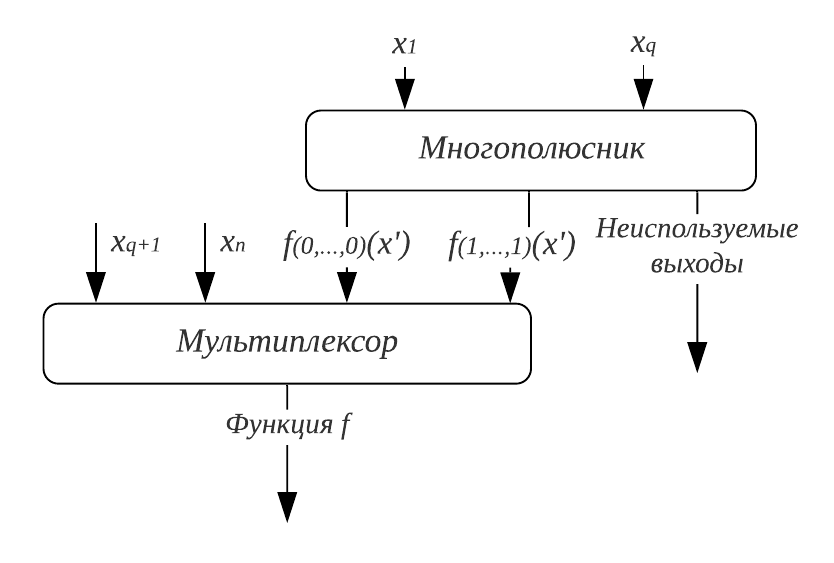
\includegraphics[width=0.9\columnwidth]{pics/osn27_oki.png}

Сложность многополюсника от $q$ переменных: $L(\Sigma') \leqslant 2^{2^q} - q $ (следует из леммы)

Сложность мультиплексора от $n-q$ переменных: $L(\Sigma'') \leqslant 2^{n - q + 2} - 3$

Полагая $q = \lfloor \log_2(n - 2\log_2 n) \rfloor$ получаем в результате преобразований: 
$$ L(\Sigma_f) \leqslant 2^{2^q} + 4\cdot 2^{n - q} \leqslant \frac{8 \cdot 2^n}{n - 2\log n} + O(\frac{2^n}{n^2}) $$

\textbf{Таким образом, верна оценка сложности СФЭ: }$L^C(n) \lesssim 8 \cdot \frac{2^n}{n}$

% -------- source --------

\vfill\null
\columnbreak
%---------------------3--------------------
\textbf{\LARGE osn 26. Теоремы существования и единственности решения задачи Коши для обыкновенного дифференциального уравнения первого порядка, разрешенного относительно производной.}

Пусть функция $f(t,y)$ определена и непрерывна в прямоугольнике 
П$ = \{(t, y) : |t - t_0| \leqslant T, |y - y_0| \leqslant A\}$.

Рассмотрим на отрезке $[t_0 - T ; t_0 + T ]$ дифференциальное уравнение с условием:
\begin{equation}
    y'(t) = f(t, y(t))
    \label{eq3}
\end{equation}
\begin{equation}
    y(t_0) = y_0
    \label{eq4}
\end{equation}

Требуется определить функцию $y(t)$, удовлетворяющую уравнению (\ref{eq3}) и условию (\ref{eq4}).

Эта задача называется \textbf{задачей с начальным условием или задачей Коши}. Рассмотрим отрезок $[t_1, t_2]$ такой, что $t_0 - T \leqslant t_1 < t_2 \leqslant t_0 + T,~t_0 \in [t_1, t_2]$.

\textbf{Опр.} Функция $y(t)$ называется \textbf{решением задачи Коши} (\ref{eq3}), (\ref{eq4}) на отрезке $[t_1, t_2]$, если $y(t) \in C^1[t_1, t_2],~|y(t) - y_0| \leqslant A$ для $t \in [t_1, t_2],~y(t)$ удовлетворяет уравнению (\ref{eq3}) для $t \in [t_1, t_2]$ и (\ref{eq4}).

Рассмотрим на отрезке $[t_0 - T,t_0 + T]$ уравнение относительно неизвестной функции $y(t)$:
\begin{equation}
    y(t) = y_0 + \int\limits_{t_0}^{t}f(\tau, y(\tau))d\tau
    \label{eq5}
\end{equation}

\textbf{Лемма 1.} Функция $y(t)$ является решением задачи Коши (\ref{eq3}), (\ref{eq4}) на отрезке $[t_1, t_2] \iff$ когда $y(t) \in C[t_1, t_2],~|y(t) - y_0| \leqslant A$ для $t \in [t_1, t_2]$ и $y(t)$ удовлетворяет уравнению (\ref{eq5}) для $t \in [t_1, t_2]$.

\begin{proof} ($\implies$) Пусть функция $\overline{y}(t)$ является решением задачи с начальным условием (\ref{eq3}), (\ref{eq4}) на отрезке $[t_1, t_2]$. Из определения решения следует, что $\overline{y}(t) \in C[t_1,t_2],~|\overline{y}(t)-y_0| \leqslant A$ для $t \in [t_1,t_2]$. Покажем, что $\overline{y}(t)$ удовлетворяет уравнению (\ref{eq5}) для $t \in [t_1, t_2]$. Интегрируя (\ref{eq3}) от $t_0$ до $t$ получим:
$$ \int\limits_{t_0}^{t}\overline{y}'(\tau)d\tau = \int\limits_{t_0}^{t}f(\tau, \overline{y}(\tau))d\tau,~t\in[t_1,t_2]$$
Учитывая условие (\ref{eq4}), имеем:
$$ \overline{y}(t) = y_0 + \int\limits_{t_0}^{t}f(\tau, \overline{y}(\tau))d\tau,~t\in[t_1,t_2]$$
Следовательно, функция $\overline{y}(t)$ удовлетворяет интегральному уравнению (\ref{eq5}) при $t \in [t_1, t_2]$.

($\impliedby$) Пусть функция $\overline{y}(t)$ такова, что $\overline{y}(t) \in C[t_1, t_2],~|y(t) - y_0| \leqslant A$ для $t \in [t_1, t_2]$ и $\overline{y}(t)$ удовлетворяет уравнению (\ref{eq5}) для $t \in [t_1, t_2]$, то есть:
\begin{equation}
    \overline{y}(t) = y_0 + \int\limits_{t_0}^{t}f(\tau, \overline{y}(\tau))d\tau,~t\in[t_1,t_2]
    \label{eq6}
\end{equation}
Покажем, что $y(t)$ является решением задачи с начальным условием (\ref{eq3}), (\ref{eq4}). 

Положив в (\ref{eq6}) $t = t_0$, получим, что $\overline{y}(0) = y_0$. Следовательно условие (\ref{eq4}) выполнено. Так как функция $\overline{y}(t)$ непрерывна на $[t_1,t_2]$, то правая часть равенства (\ref{eq6}) непрерывно дифференцируема на $[t_1, t_2]$ как интеграл с переменным верхним пределом $t$ от непрерывной функции $f(\tau,\overline{y}(\tau)) \in C[t_1,t_2]$. Следовательно, $\overline{y}(t)$ непрерывно дифференцируема на $[t_1, t_2]$. Дифференцируя (\ref{eq6}), получим, что $\overline{y}(t)$ удовлетворяет (\ref{eq3}).
\end{proof}

\textbf{Опр.} Функция $f(t,y)$, заданная в прямоугольнике П, \textit{удовлетворяет в П условию Липшица} по $y$, если $|f(t,y_1)-f(t,y_2)| \leqslant L|y_1 -y_2|,~\forall(t,y_1),(t,y_2) \in$ П, где $L$ --- положительная постоянная.

\textbf{Лемма Гронуолла-Беллмана.} Пусть функция $z(t) \in C[a,b]$ и такова, что $0 \leqslant z(t) \leqslant c+d \Big|\int\limits_{t_0}^{t}z(\tau)d\tau\Big|,~t\in[a, b]$, где постоянная $c$ неотрицательна, постоянная $d$ положительна, а $t_0$ --- произвольное фиксированное число на отрезке $[a, b]$. Тогда $z(t) \leqslant c e^{d|t-t_0|},~t \in [a, b]$.

\textbf{Теорема (единственности).} Пусть функция $f(t,y)$ непрерывна в П и удовлетворяет в П условию Липшица по $y$.
Если $y_1(t),~y_2(t)$ --- решения задачи Коши (\ref{eq3}), (\ref{eq4}) на отрезке $[t_1, t_2]$, то $y_1(t) = y_2(t)$ для $t \in [t_1, t_2]$.

\begin{proof} Так как $y_1(t)$ и $y_2(t)$ --- решения задачи Коши (\ref{eq3}), (\ref{eq4}), то из Леммы 1 следует, что они являются решениями интегрального уравнения (\ref{eq5}).

То есть:
$$y_1(t) = y_0 + \int\limits_{t_0}^{t}f(\tau, y_1(\tau))d\tau,~t\in[t_1,t_2],$$
$$y_2(t) = y_0 + \int\limits_{t_0}^{t}f(\tau, y_2(\tau))d\tau,~t\in[t_1,t_2].$$
Вычитая второе уравнение из первого и оценивая разность по модулю и используя условие Липшица, получаем:
$|y_1(t) - y_2(t)| = \Big| \int\limits_{t_0}^{t}f(\tau, y_1(\tau))d\tau - \int\limits_{t_0}^{t}f(\tau, y_2(\tau))d\tau \Big| \leq \Big| \int\limits_{t_0}^{t}|f(\tau, y_1(\tau)) - f(\tau, y_2(\tau))|d\tau \Big| \leq L\Big| \int\limits_{t_0}^{t}|y_1(\tau) - y_2(\tau)|d\tau \Big|$

Обозначив $z(t) = |y_1(t) - y_2(t)|$, перепишем последнее неравенство следующим образом:

$0 \leqslant z(t) \leqslant L\Big|\int\limits_{t_0}^{t}z(\tau)d\tau \Big|,~t \in [t_1,t_2].$

Применяя лемму Гронуолла-Беллмана с $c = 0$ и $d = L$, имеем
$z(t) = 0,~t \in [t_1, t_2]$. Следовательно, $y_1(t) = y_2(t),~t \in [t_1, t_2].$
\end{proof} 

\textbf{Теорема (существования) ((локальная)).}
Пусть функция $f(t,y)$ непрерыв на в П, удовлетворяет в П условию Липшица по $y$ и $|f(t,y)| \leq M, (t,y) \in$ П. Тогда на отрезке $[t_o - h, t_0 + h]$, где $h = min\{T, \frac{A}{M}\}$, существует функция $y(t)$ такая, что $y(t) \in C^1 [t_0-h, t_0 + h], |y(t) - y_0| \leq A, t \in [t_0 - h, t_0 + h]$,\newline
$y'(t) = f(t,y(t)), t \in [t_0 - h, t_0 + h]$
$y(t_0) = y_0$\newline

\textit{Следует отметить, что мы можем доказать теорему существования не на всем исходном отрезке $[t0 - T , t0 + T ]$, а на некотором, вообще говоря, меньшем. Поэтому эта теорема часто называется} \textbf{локальной} \textit{теоремой существования решения задачи Коши.}



% -------- source --------
\bigbreak
[\cite[page 25-30]{denisov}]
\vfill\null
\columnbreak
%---------------------
\end{multicols}
\end{tcolorbox}
% --- END OF PAGE ----



% --- BEGIN OF PAGE ----
\newpage
\begin{tcolorbox}[colback=white, left=0mm, right=0mm]
\begin{multicols}{4}
%---------------------0--------------------
\textbf{\LARGE osn 33. Задача Коши для уравнения колебания струны. Формула Даламбера.}

\textbf{Задача Коши для уравнения колебания струны.}

$$\begin{cases}
u_{tt}=a^2u_{xx}+f(x,t)&\\
u(x,0)=\varphi(x)&\\
u_t(x,0)=\psi(x)&\\
\end{cases}$$ где $t>0,~a>0,~u(x,t)\in C^2(t > 0, x\in \mathbb{R})\cap C^1(t \geqslant 0, x\in \mathbb{R})$.

\bigbreak
\textit{Физическая интерпретация:} уравнение малых поперечных колебаний струны. $u(x,t)$ -- положение точки струны с координатой $x$ в момент времени $t$. Если концы струны закреплены, то $u(0,t)=0, u(l,t)=0$. Так как процесс колебаний струны зависит от ее начальной формы и распределения скоростей, то задают начальные условия. $a = \sqrt{\frac{T_0}{\rho}}$, где $T_0$ -- величина натяжения (не зависит от $x$, $\rho$ -- линейная плотность струны. $f(x,t)$ -- плотность внешних сил.

\bigbreak
Далее будем рассматривать $f(x,t) = 0$.
\bigbreak

(\textit{Представим что $\frac{\partial^2u}{\partial t^2} = \frac{d^2u}{dt^2}$ и $\frac{\partial^2u}{\partial x^2} = \frac{d^2u}{dx^2}$:
$\frac{d^2u}{dt^2} = a^2\frac{d^2u}{dx^2} \implies$
${d^2udx^2 = a^2dt^2d^2u} \implies$
${dx^2 = a^2dt^2}$.})
Характеристическое уравнение: $dx^2-a^2dt^2=0$. \\
$dx - adt=0, ~ dx+adt = 0 \implies x-at=C_1 = const, ~ x+at=C_2 = const$

Сделаем замену переменных: $$x+at=\xi,~x-at=\eta$$
$$\xi_x=1, ~ \xi_{xx}=0, ~ \eta_x = 1,  ~ \eta_{xx} = 0,$$
$$\xi_t=a, ~ \xi_{tt}=0, ~ \eta_t = -a, ~ \eta_{tt} = 0.$$

Тогда:
$$u_x=u_{\xi}\cdot\xi_x+u_{\eta}\cdot\eta_x,$$
$$u_t=u_{\xi}\cdot\xi_t+u_{\eta}\cdot\eta_t,$$
$$u_{xx}=u_{\xi\xi}\cdot\xi_x^2+2u_{\xi\eta}\cdot\xi_x\cdot\eta_x+u_{\xi}\cdot\xi_{xx}+u_{\eta\eta}\cdot\eta_x^2+u_{\eta}\cdot\eta_{xx},$$
$$u_{tt}=u_{\xi\xi}\cdot\xi_t^2+2u_{\xi\eta}\cdot\xi_t\cdot\eta_t+u_{\xi}\cdot\xi_{tt}+u_{\eta\eta}\cdot\eta_t^2+u_{\eta}\cdot\eta_{tt}.$$

Подставляем в уравнение $u_{tt}=a^2u_{xx}$:
$$u_{\xi\xi}\cdot\xi_t^2+2u_{\xi\eta}\cdot\xi_t\cdot\eta_t+\displaystyle\underbrace{u_{\xi}\cdot\xi_{tt}}_{\text{= 0}}+u_{\eta\eta}\cdot\eta_t^2+\displaystyle\underbrace{u_{\eta}\cdot\eta_{tt}}_{\text{= 0}}=$$ $$=a^2(u_{\xi\xi}\cdot\xi_x^2+2u_{\xi\eta}\cdot\xi_x\cdot\eta_x+\displaystyle\underbrace{u_{\xi}\cdot\xi_{xx}}_{\text{= 0}}+u_{\eta\eta}\cdot\eta_x^2+\displaystyle\underbrace{u_{\eta}\cdot\eta_{xx}}_{\text{= 0}})$$
Преобразуем:
$$a^2u_{\xi\xi}-2a^2u_{\xi\eta}+a^2u_{\eta\eta}=a^2u_{\xi\xi}+2a^2u_{\xi\eta}+a^2u_{\eta\eta}$$
$$4a^2u_{\xi\eta}=0,   a>0$$
Получаем: $u_{\xi\eta}=0$

Найдем общий интеграл этого уравнения: $u_{\eta}(\xi, \eta)=f^*(\eta)$, где $f^*(\eta)$ - некоторая функция только переменного $\eta$.

Интегрируя это равенство по $\eta$ при фиксированном $\xi$, получим:
\begin{equation}
    u(\xi, \eta)=\int f^*(\eta)d\eta = f_1(\xi) + f_2(\eta)
    \label{isuvdno}
\end{equation}

Обратно, каковы бы ни были дважды дифференцируемые функции $f_1$ и $f_2$, функция $u(\xi,\eta)$, определяемая формулой (\ref{isuvdno}), представляет собой решение уравнения $u_{\xi\eta}=0$. Так как всякое решение уравнения $u_{\xi\eta}=0$ может быть представлено в виде (\ref{isuvdno}) при соответствующем выборе $f_1$ и $f_2$, то формула (\ref{isuvdno}) является общим интегралом этого уравнения. Следовательно, функция $$u(x, t) = f_1(x+at) + f_2(x-at)$$ является общим интегралом уравнения $u_{tt}=a^2u_{xx}$.

Удовлетворим начальным условиям:
$$\begin{cases}
u(x,0)=f_1(x)+f_2(x)=\varphi(x)&\\
u_t(x,0)=-af_1'(x)+af_2'(x)=\psi(x)&\\
\end{cases}
$$

Проинтегрируем второе равенство, получим:
$$\begin{cases}
f_1(x)+f_2(x)=\varphi(x)&\\
f_1(x)-f_2(x)=\frac{1}{a}\int\limits_{x_0}^{x}\psi(\alpha)d\alpha + C&\\
\end{cases}
$$

Сложим и вычтем два полученных равенства:
$$\begin{cases}
f_1(x)=\frac{1}{2}\varphi(x)+\frac{1}{2a}\int\limits_{x_0}^{x}\psi(\alpha)d\alpha + \frac{C}{2}&\\
f_2(x)=\frac{1}{2}\varphi(x)-\frac{1}{2a}\int\limits_{x_0}^{x}\psi(\alpha)d\alpha - \frac{C}{2}&\\
\end{cases}
$$

Подставим в $u(\xi, \eta) = f_1(x+at) + f_2(x-at)$ найденные выражения для $f_1, f_2$:
$$u(x,t)=\frac{\varphi(x+at)+\varphi(x-at)}{2} + \frac{1}{2a}\left(\int\limits_{x_0}^{x+at}\psi(\alpha)d\alpha - \int\limits_{x_0}^{x-at}\psi(\alpha)d\alpha\right)$$

Окончательно:
$$u(x,t)= \frac{\varphi(x+at)+\varphi(x-at)}{2} + \frac{1}{2a}\int\limits_{x-at}^{x+at}\psi(\alpha)d\alpha$$

Полученная формула -- \textbf{формула Даламбера}.

\textbf{Теорема о применимости формулы Даламбера.} Пусть $\varphi(x) \in C^2(-\infty, \infty), \psi \in C^1[0,+\infty), a > 0$. Тогда формула Даламбера представляет единственное решение задачи Коши для уравнения колебания струны.

% -------- source --------
\bigbreak
[\cite[page 50-52]{urmati_tikhonov}]
\vfill\null
\columnbreak
%---------------------1--------------------
\textbf{\LARGE osn 34. Постановка краевых задач для уравнения теплопроводности.  Метод разделения переменных для решения первой краевой задачи.}

Краевые задачи для уравнения теплопроводности представляют собой математические модели процессов распространения тепла, например, в стержне.
    
$u(x,t)$ --- температура в сегменте с координатами $x$ во время $t$.

$F(x, t)$ --- плотность тепловых источников, $a^2 = \frac{k}{c\rho}$ --- коэффициент температуропроводности, $f(x,t)=\frac{F(x,t)}{c\rho}$ , $c$ --- удельная теплоемкость, $k$ --- коэффициент теплопроводности, $\rho$ --- плотность.

\bigbreak

Одномерное уравнение теплопроводности:

$u_t(x,t)=a^2u_{xx}(x,t)+f(x,t)$


\textbf{Основные типы задач:}
\begin{itemize}
    \item \textbf{Первая краевая задача.}
    
    $\begin{cases}
    u_t(x,t)=a^2u_{xx}(x,t)+f(x,t),~0<x<l,~t>0&\\
    u(0,t)=\mu_1(t),~t\geqslant0&\\
    u(l,t)=\mu_2(t)&\\
    u(x,0)=\varphi(x),~0\leqslant x\leqslant l&\\
    \end{cases}$
    \item \textbf{Вторая краевая задача.}
    
    $\begin{cases}
    u_t(x,t)=a^2u_{xx}(x,t)+f(x,t),~0<x<l,~t>0&\\
    u_x(0,t)=\nu_1(t),~t\geqslant0&\\
    u_x(l,t)=\nu_2(t)&\\
    u(x,0)=\varphi(x),~0\leqslant x\leqslant l&\\
    \end{cases}$
    \item \textbf{Смешанная краевая задача.} --- одно из краевых условий задано функцией $u(0,t)$ или $u(l,t)$, а другое производной $u$ по $x$.
\end{itemize}

$u(x,t)$ --- \textbf{решение 1-ой краевой задачи} для уравнения теплопроводности, если:
\begin{enumerate}
    \item $u(x,t)\in C([0,l]\times[0,+\infty))$;
    \item $u(x,t)\in C^2((0,l)\times(0,+\infty))$;
    \item $u(x,t)$ удовлетворяет условиям 1-ой краевой задачи.
\end{enumerate}

\bigbreak
Далее будем рассматривать $f(x,t)=0$.

\bigbreak
\textbf{Метод разделения переменных для решения первой краевой задачи.}

$\begin{cases}
    u_t(x,t)=a^2u_{xx}(x,t),~0<x<l,~t>0&\\
    u(0,t)=0,~t\geqslant0&\\
    u(l,t)=0&\\
    u(x,0)=\varphi(x),~0\leqslant x\leqslant l&\\
\end{cases}$

\bigbreak
Будем искать решение в виде $u(x,t)=X(x)T(t)$. Рассмотрим задачу с однородными начальными и краевыми условиями:

$\begin{cases}
XT'=a^2X''T&\\
X(0)T(t)=0&\\
X(l)T(t)=0&\\
\end{cases} \rightarrow 
\begin{cases}
\frac{T'}{a^2T}=\frac{X''}{X}=-\lambda&\\
X(0)=X(l)=0&\\
\end{cases}$

\bigbreak
Получаем две задачи:
\begin{enumerate}
    \item Задача Штурма-Лиувилля:
    
    $\begin{cases}
    X''+\lambda X=0&\\
    X(0)=X(l)=0&\\
    \end{cases}$
    
    Рассматриваем 3 случая: $\lambda<0,~\lambda=0,~\lambda>0$. При $\lambda>0$ получаем $\lambda_n=(\frac{\pi n}{l})^2,~X_n(x)=\sin(\frac{\pi n x}{l}),~n\in\mathbb{N}$
    
    \item $T'+(\frac{\pi n a}{l})^2 T = 0$
    
    Решение: $T_n(t)=a_n e^{-(\frac{\pi n a}{l})^2t},~n\in\mathbb{N}$
\end{enumerate}

\bigbreak
Получаем решение: $u(x,t)=\displaystyle\sum_{n=1}^{\infty} a_n e^{-(\frac{\pi n a}{l})^2t} \sin(\frac{\pi n x}{l})$

Для нахождения $a_n$ используем начальное условие.
Так как $\{\sin(\frac{\pi n x}{l})\}$ --- замкнутая полная система функций, то $\forall$ кусочно-дифференцируемую функцию можно разложить в ряд Фурье:

$$\varphi(x) = \displaystyle\sum_{n=1}^{\infty} \varphi_n \sin(\frac{\pi n x}{l}),~\varphi_n=\frac{2}{l}\int\limits_0^l\varphi(\xi)\sin(\frac{\pi n \xi}{l})d\xi$$

Так как $u(x,0) = \varphi(x)$, получаем $a_n = \varphi_n,~n\in\mathbb{N}$. Таким образом, получаем решение:

$$u(x,t)=
\displaystyle\sum_{n=1}^{\infty} \frac{2}{l}\int\limits_0^l\varphi(\xi)\sin \left( \frac{\pi n \xi}{l} \right)d\xi \cdot e^{-(\frac{\pi n a}{l})^2t} \sin \left(\frac{\pi n x}{l} \right)$$

\bigbreak
Для существования решения достаточно потребовать, чтобы $\varphi\in C^2[0,l]$ и $\varphi(0)=\varphi(l)=0$.

\bigbreak
Остальные случаи:
\begin{itemize}
    \item $X'(0)=X(l)=0$: $\lambda_n=\left(\frac{\pi(2n+1)}{2l}\right)^2, X_n=\cos\sqrt{\lambda_n}, n=0,1,2,\dots$ \\
    \item $X(0)=X'(l)=0$: $\lambda_n=\left(\frac{\pi(2n+1)}{2l}\right)^2, X_n=\sin\sqrt{\lambda_n}, n=0,1,2,\dots$ \\
    \item $X'(0)=X'(l)=0$: $\lambda_n=\left(\frac{\pi n}{l}\right)^2, X_n=\cos\sqrt{\lambda_n}, n=1,2,\dots; X_0=1$ \\
\end{itemize}

% -------- source --------
\bigbreak
[\cite[page 200-202]{urmati_tikhonov}]
\vfill\null
\columnbreak
%---------------------2--------------------
\vfill\null
\columnbreak
%---------------------3--------------------
\vfill\null
\columnbreak
%---------------------
\end{multicols}
\end{tcolorbox}
% --- END OF PAGE ----



% -------------------------------------------------------------------- DOP -


% --- BEGIN OF PAGE ----
\newpage
\begin{tcolorbox}[colback=white, left=0mm, right=0mm]
\begin{multicols}{4}
%---------------------0--------------------
\textbf{\LARGE dop 1. Необходимые условия экстpемума функции нескольких пеpеменных. Достаточные условия.}

\rule{275pt}{0.5pt}
\begin{center}
    \textbf{Вспомогательная теория}
\end{center}

\textbf{Вторая теорема Вейерштрасса:} Если функция $f(x)$ непрерывна на некотором замкнутом и ограниченном множестве, то она достигает на этом множестве своих точных верхней и нижней граней.

\textbf{Теорема Ферма:} Если $f(x)$ дифференцируема в точке $x=c$ и имеет в этой точке локальный экстремум, то $f'(c) = 0$.  

\textbf{Опр:} Квадратичная форма $\Phi(h_1, h_2, \ldots, h_n) = \sum_{i=1}^n \sum_{j=1}^n a_{ij} h_i h_j$ с матрицей $A = \{a_{ij}\}$ называется:
\begin{itemize}
    \item \textbf{положительно (отрицательно) определенной}, если для $\forall \; h_1, \ldots, h_n$, одновременно не равных нулю, эта форма принимает строго положительные (отрицательные) значения;
    \item \textbf{знакоопределенной}, если она является либо положительно, либо отрицательно определенной;
    \item \textbf{знакопеременной}, если она принимает как строго положительные, так и строго отрицательные значения;
    \item \textbf{квазиопределенной}, если она принимает либо только неотрицательные, либо только неположительные значения, но при этом обращается в нуль для некоторых $h_1, \ldots, h_n$, одновременно не равных нулю.
\end{itemize}

\textbf{Критерий Сильвестра знакоопределенности квадратичной формы:}
\begin{enumerate}
    \item Квадратичная форма $\Phi$ с симметричной матрицей $A$ является \textbf{положительно} определенной $\Leftrightarrow$ все главные миноры матрицы $A$ положительны;
    \item Квадратичная форма $\Phi$ с симметричной матрицей $A$ является \textbf{отрицательно} определенной $\Leftrightarrow$ знаки главных миноров матрицы $A$ чередуются, причем $A_1 = a_{11} < 0$.
\end{enumerate}
\rule{275pt}{0.5pt} \\

\fbox{\textbf{Опр. 1:}} Точка $x_0 = (x_{01}, \ldots, x_{0n})$, внутренняя для области определения функции $f(x) = f(x_1, \ldots, x_n)$, называется точкой \textbf{локального экстремума} функции $f$, если для любой точки $x$ из некоторой ее окрестности $U = U(x_0)$ разность $\Delta f = f(x) - f(x_0)$ отлична от нуля и сохраняет знак. В частности, если $\Delta f> 0$, то это точка \textbf{локального минимума}, если $\Delta f < 0$, то это точка \textbf{локального максимума}.\\

\textbf{Теорема 1 \textit{(необходимое условие)}:} Если у функции $f(x)$ в точке $x_0$ существуют все частные производные $f'_{x_k}$, и эта точка является точкой локального экстремума, то все частные производные в ней равны нулю, то есть $f'_{x_k}(x_0) = 0, \; k = 1, \ldots, n$.

$\blacktriangleright\;$ Зафиксируем у функции $f(x)$ все переменные, кроме $x_k \;(1\leq k\leq n)$, и рассмотрим функцию $\varphi(x_k) = f(x_{01}, \ldots, x_{0 k-1}, x_k, x_{0 k+1}, \ldots, x_{0 n})$ -- функцию одной переменной. Очевидно, что для функции $\varphi(x_k)$ точка $x_{0k}$ является также точкой локального экстремума. По теореме Ферма имеем, что $\varphi'(x_{0k}) = 0 \;\implies\; f'_{x_k} (x_0) = 0, \; 1\leq k \leq n$.\;$\blacksquare$\\

\fbox{\textbf{Опр. 2:}} Точка $x_0 = (x_{01}, \ldots, x_{0n})$ называется \textbf{стационарной} для функции $f(x) = f(x_1, \ldots, x_n)$, если она внутренняя для ее области определения, и все частные производные в ней определены и равны нулю: $f'_{x_k}(x_0) = 0, \; k = 1, \ldots, n$.\\

\textbf{Теорема 2 \textit{(достаточные условия)}:} Пусть функция $f(x) = f(x_1, \ldots, x_n)$ от $n$ независимых переменных один раз дифференцируема в некоторой окрестности точки $x_0 = (x_{01}, \ldots, x_{0n})$, и дважды дифференцируема в самой точке $x_0$. Пусть $x_0$ -- стационарная точка, то есть дифференциал функции $f$ равен нулю в точке $x_0$ ($d f(x_0) = 0$). Тогда если второй дифференциал $d^2 f(x_0)$ представляет собой знакоопределенную квадратичную форму, то $x_0$ -- точка локального экстремума. При этом, если форма $d^2f(x_0)$ положительно (отрицательно) определена, то $x_0$ -- точка локального миниммума (максимума). Если же квадратичная форма $d^2 f(x_0)$ знакопеременна, то локального экстремума в точке $x_0$ нет.

$\blacktriangleright\;$ Разложим разность $\Delta f$ по формуле Тейлора при $n = 2$ с остаточным членом в форме Пеано:
$$
\Delta f = f(x) - f(x_0) = d f(x_0) + \frac{d^2 f(x_0)}{2!} + \overline{o}(\|\Delta x\|^2) =$$
$$= \{ d f(x_0) = 0\} = \frac{1}{2!}\,\sum_{i = 1}^n \sum_{j =1}^n f''_{x_i x_j}(x_0) \Delta x_i \Delta x_j + \overline{o}(\|\Delta x\|^2).
$$
Обозначим $h_i = \frac{\Delta x_i}{\|\Delta x\|}, \; a_{ij} = f''_{x_i x_j}(x_0), \; \alpha = \alpha (\|x\|) = \frac{\overline{o}(\|\Delta x\|^2)}{\|\Delta x\|^2}$. 
Отметим, что $\alpha(\|x\|)$ -- бесконечно малая при $\|\Delta x\| \to 0$. 
Тогда $\Delta f$ представляется в виде $\Delta f = \frac{1}{2}\|\Delta x\|^2\, \left( \sum_{1\leq i, j \leq n} a_{ij} h_i h_j + \alpha\right)$. 
Заметим, что вектор $h = \{ h_1, \ldots, h_n\}$ имеет норму $\|h\| = \sqrt{h_1^2 + \ldots + h_n^2} = 1$, то есть это элемент единичной сферы $S^{n-1}$ пространства $\mathbb{R}^n$.

\textbf{1)} Рассмотрим случай, когда $d^2 f(x_0)$ -- \textbf{положительно определенная} квадратичная форма. 
В этом случае квадратичная форма $\Phi(h) = \sum_{1\leq , j \leq n} a_{ij}h_i h_j$ -- также положительно определенная непрерывная функция на единичной сфере $S^{n-1}$. 
Сфера $S^{n-1}$ является замкнутым ограниченным множеством в $\mathbb{R}^n$, следовательно, по второй теореме Вейерштрасса функция $\Phi(h)$ достигает на $S^{n-1}$ своего инфимума, то есть существует такая точка $\xi = (\xi_1, \ldots, \xi_n) \in S^{n-1}$, в которой $\Phi(\xi) = \inf_{h \in S^{n-1}} \Phi(h) = \mu$. 
Поскольку всюду на сфере $\Phi(h) > 0$, то $\Phi(h) \leq \Phi(\xi) = \mu > 0$. Воспользовавшись этим, получаем 
$$
\Delta f = \frac{1}{2} \|\Delta x\|^2 (\Phi(h) + \alpha) \geq \frac{1}{2} \|\Delta x\|^2 (\mu + \alpha).
$$
Так как $\alpha \to 0$ при $\|\Delta x\| \to 0$, то $\exists \, \delta = \delta (\mu) > 0 \,:\; \|\Delta x\| < \delta \implies |\alpha| < \frac{\mu}{2}$.
При этих условиях 
$$
\Delta f \geq \frac{1}{2} \|\Delta x\|^2 (\mu + \alpha) > \frac{1}{2} \|\Delta x\|^2 (\mu - \frac{\mu}{2}) = \frac{1}{2} \|\Delta x\|^2 \frac{\mu}{2} > 0.
$$
Итак $\forall\, x \in \mathbb{R}^n : \; \|\Delta x\| < \delta \implies \Delta f > 0 $. Следовательно, точка $x_0$ -- точка локального минимума по определению 1.

\textbf{2)} В случае \textbf{отрицательно определенной} квадратичной форму $d^2 f(x_0)$ совершенно аналогично доказывается, что $x_0$ -- точка локального максимума.

\textbf{3)} Пусть теперь $d^2 f(x_0)$ -- \textbf{знакопеременная} квадратичная форма. Тогда имеем 
$$
\Delta f = \frac{1}{2} \rho^2 (\Phi(h) + \alpha),\quad \rho = \|\Delta x\|,
$$
где $\Phi(h)$ -- знакопеременная квадратичная форма на единичной сфере $S^{n-1}$. 
Следовательно $ \exists \; h', \; h'' \in S^{n-1} \,: \; \Phi(h') <0, \; \Phi(h'') > 0$. 
При этом заметим, что $\alpha = \alpha (\rho)$ и $\alpha \to 0$ при $\rho \to 0$, а $\Phi(h)$ от $\rho$ не зависит.
Поэтому взяв $\rho_0$ достаточно малым, можно добиться, чтобы $|\alpha| = |\alpha(\rho_0)| < \min \big\{|\Phi(h')| / 2, \;  |\Phi(h'')| / 2\big\}$. 
При этих условиях будет одновременно $ \Phi(h') + \alpha(\rho_0) < 0, \; \Phi(h'') + \alpha(\rho_0) > 0$. 
Тогда для точек $x' = x_0 + \rho_0 h', \; x'' = x_0 + \rho_0 h''$ будем иметь
$$
(\Delta f)_1 = f(x') - f(x_0) = \frac{1}{2} \rho_0^2 \big(\Phi(h') + \alpha(\rho_0) \big) < 0,
$$
$$
(\Delta f)_2 = f(x'') - f(x_0) = \frac{1}{2} \rho_0^2 \big(\Phi(h'') + \alpha(\rho_0) \big) > 0.
$$
Итак, приращение функции меняет знак $\implies$ точка $x_0$ не является точкой экстремума функции $f(x)$. $\;\blacksquare$\\

\textbf{Замечание:} В случаях \textbf{квази-определенности} (полуопределенности) квадратичной формы второго дифференциала $d^2 f(x_0)$ ответ о существовании локального экстремума в точке $x_0$ дать нельзя.


% -------- source --------
\bigbreak
[\cite[page 69-74]{Sadovn_func_mhogih}]
\vfill\null
\columnbreak
%---------------------1--------------------
\textbf{\LARGE dop 3. Почленное интегрирование и дифференцирование функциональных рядов.}

\textbf{Равномерная сходимость на множестве}

\mathLet \ ф.п. $f_n(x) \xrightarrow[\{x\}]{}  f(x)$, где $\{x\} \in E^m$ \\
Ф.п. $\{f_n(x)\}$ сходится к функции $f(x)$ \textbf{равномерно на множестве} $\{x\}$ \ $f_n(x)\underset{\{x\}}{\rightrightarrows}f(x)$, если для $\forall \varepsilon > 0 \ \exists$ номер $N(\varepsilon)$: для $\forall n: n \ge N(\varepsilon)$ и для $\forall x \in \{x\}$ выполняется

\begin{equation}
    |f_n(x) - f(x)| < \varepsilon
\end{equation}

\bigbreak
Функциональный ряд называется \textbf{равномерно сходящимся} на множестве $\{x\}$ к сумме $S(x)$, если п-ть $\{S_n(x)\}$ его частичных сумм сходится равномерно на $\{x\}$ к предельной функции $S(x)$.

\bigbreak
\textbf{Критерий Коши равномерной сх-ти.} \\
Ф.п. $\{f_n(x)\}\underset{\{x\}}{\rightrightarrows}f(x) \Leftrightarrow $ для $\forall \varepsilon > 0 \ \exists N(\varepsilon): |f_{n+p}(x) - f_n(x)| < \varepsilon \text{ при } \forall n: n \ge N(\varepsilon), \forall p \in \mathbb{N}, \forall x \in \{x\}$.

\bigbreak
\textbf{Почленный переход к пределу (теорема)}. \\
Если ф.п. $\{f_n(x)\} \underset{\{x\}}{\rightrightarrows}f(x)$ и для $\forall n \ \exists \lim_{x \rightarrow x_0}{f_n(x)} $, то и предельная функция $f(x)$ имеет предел в точке $x_0$, причем
\begin{equation}
    \lim_{x \rightarrow x_0}{f(x)} = \lim_{x \rightarrow x_0}{(\lim_{n \rightarrow \infty}{f_n(x)})} = \lim_{n \rightarrow \infty}{(\lim_{x \rightarrow x_0}{f_n(x)})}
\end{equation}

\bigbreak
\textbf{Почленное интегрирование (теорема).} \\
Если ф.п. $\{f_n(x)\} \underset{[\,a,b]\, }{\rightrightarrows}f(x)$ и если $\forall f_n(x)$ интегрируема на $[\,a,b]\,$, то и предельная функция $f(x)$ интегрируема на $[\,a,b]\,$.

\begin{equation}
    \lim_{n \rightarrow \infty}{\int_{a}^{b} f_n(x) \,dx} =  \int_{a}^{b} \lim_{n \rightarrow \infty}{f_n(x)} \,dx = \int_{a}^{b} f(x) \,dx.
\end{equation}

\begin{proof}
Докажем, что предельная функция $\boldsymbol{f(x)}$ \textbf{интегрируема} на $[\,a,b]\,$ \\

Фиксируем $\forall \varepsilon > 0$. Достаточно доказать, что для $f(x)$ найдется хотя бы одно разбиение сегмента $[\,a,b]\,$: $S-s<\varepsilon$, где $S$ и $s$ - верхняя и нижняя суммы разбиения для функции $f(x)$. \\ 

Для этого достаточно доказать, что для выбранного $\varepsilon$ $\exists$ номер $n$: для $\forall$ разбиения сегмента $[\,a,b]\,$ выполняется
\begin{equation}\label{S-s<e}
    S-s \le (S_n - s_n) + \frac{\varepsilon}{2},
\end{equation}
где $S,s-$ суммы для $f(x)$, $S_n,s_n -$ суммы для $f_n(x)$. \\

Так как $f_n(x)$ интегрируемы на $[\,a,b]\,$, то можно выбрать разбиение: $S_n-s_n < \frac{\varepsilon}{2}$. Если для некоторого разбиения для некоторого $n$ будет д-но (\ref{S-s<e}), то будет верно $S -s < \varepsilon$, а это и будет означать интегрируемость предельной функции $f(x)$ на $[\,a,b]\,$. \\

Рассмотрим произвольное разбиение $\{x_k\} (k=1,2, ..., m)$ сегмента $[\,a,b]\,$ и обозначим символом $\omega_k(f_n) $ колебание на $k$-м частичном сегменте $[\,x_{k-1}, x_k]\,$ функции $f_n(x)$ (колебание функции $f(x)$ на сегменте $X$ есть разность $\sup_{x \in X}{f(x)} - \inf_{x \in X}{f(x)}$). \\

Неравенство (\ref{S-s<e}) будет доказано, если для достаточно большого $n$ будет выполнено:
\begin{equation}\label{wk<wkn}
    \omega_k(f) \le \omega_k(f_n) + \frac{\varepsilon}{2(b-a)}.
\end{equation}
Так как, умножив (\ref{wk<wkn}) на $\Delta x_k = x_k - x_{k-1}$ и суммируя получающееся неравенство по всем $k=1,2, ..., m,$ получим (\ref{S-s<e}) \\
Для $\forall n$ и $\forall$ 2-ух точек $x', x'' \in [\,x_{k-1}, x_k]\,$ справедливо $f(x') - f(x'') \equiv [\, f(x') - f_n(x')]\, +  [\, f_n(x') - f_n(x'')]\, +  [\, f_n(x'') - f(x'')]\,,$ из которого следует 

\begin{equation}\label{modules}
    |f(x') - f(x'')| \le |f(x') - f_n(x')| +  |f_n(x') - f_n(x'')| +  |f_n(x'') - f(x'')|,
\end{equation}

В силу  $\{f_n(x)\} \underset{[\,a,b]\, }{\rightrightarrows}f(x)$ для выбранного нами $\varepsilon$ $\exists n: \forall x \in [\,a,b]\,$ выполняется

\begin{equation}\label{|f_n(x)-f(x)|}
    |f_n(x) - f(x)| < \frac{\varepsilon}{4(b-a)}.
\end{equation}

Используя в правой части (\ref{modules}) неравенство (\ref{|f_n(x)-f(x)|}) получим

\begin{equation}\label{|f(x')-f(x'')|}
    |f(x') - f(x'')| \le |f_n(x') - f_n(x'')| + \frac{\varepsilon}{2(b-a)}
\end{equation}

Так как для $\forall x',x'' \in [\,x_{k-1}, x_k]\,$ справедливо $|f_n(x')-f_n(x'')| \le \omega_k(f_n)$, то из (\ref{|f(x')-f(x'')|}) получим

\begin{equation}\label{|f(x') - f(x'')|<=omega+e}
    |f(x') - f(x'')| \le \omega_k(f_n) + \frac{\varepsilon}{2(b-a)}
\end{equation}

Обозначим верхнюю и нижнюю точные грани $f(x)$ на $[\,x_{k-1}, x_k]\,$ как $M_k$ и $m_k$. В силу определения точной грани $\exists$ 2 п-ти точек $\{x_p'\}$ и $\{x_p''\}$ сегмента $[\,x_{k-1}, x_k]\,: \ \lim_{p \rightarrow \infty}{x_p'} = M_k, \lim_{p \rightarrow \infty}{x_p''} = m_k$.

В силу (\ref{|f(x') - f(x'')|<=omega+e}) для $\forall p$ справедливо
\begin{equation}\label{|f(x_p')-f(x_p'')|}
    |f(x_p')-f(x_p'')| \le \omega_k(f_n) + \frac{\varepsilon}{2(b-q)}
\end{equation}

Переходя в (\ref{|f(x_p')-f(x_p'')|}) к пределу слева получим $M_k - m_k = \omega_k(f)$. Итого в пределе получаем (\ref{wk<wkn}). Интегрируемость $f(x)$ доказана. \\

Теперь докажем почленную интегрируемость. Достаточно д-ть, что для $\forall \varepsilon > 0 \ \exists N(\varepsilon):$ для $\forall n \ge N(\varepsilon):$ $\bigg|\int_{a}^{b} f_n(x) \,dx - \int_{a}^{b} f(x) \,dx\bigg| < \varepsilon$. \\

В силу $\{f_n(x)\} \underset{[\,a,b]\, }{\rightrightarrows}f(x)$ следует, что $\exists N(\varepsilon):$ для $\forall x \in [\,a,b]\,$ и для $\forall n \ge N(\varepsilon)$ выполняется $|f_n(x)-f(x)| < \frac{\varepsilon}{2(b-a)}$. Учитывая последнее неравенство получаем:

$\bigg|\int_{a}^{b} f_n(x) \,dx - \int_{a}^{b} f(x) \,dx\bigg| = \bigg|\int_{a}^{b} [\, f_n(x) - f(x)]\,\,dx\bigg| \le \int_{a}^{b} |f_n(x) - f(x)|\,dx \le \frac{\varepsilon}{2(b-a)}\int_{a}^{b}\,dx = \frac{\varepsilon}{2} \le \varepsilon$.
\end{proof}

\bigbreak
\textbf{Почленное дифференцирование (теорема).} \\
Если каждая функция $f_n(x)$ имеет производную на $[\,a,b]\,$, причем п-ть $\{f_n'(x)\}$ cх-ся равномерно на $[\,a,b]\,$, а сама п-ть $\{f_n(x)\}$ сх-ся хотя бы в одной точке $x_0 \in [\,a,b]\,$, то $\{f_n(x)\} \underset{[\,a,b]\, }{\rightrightarrows}f(x)$, причем $\lim_{n \rightarrow \infty}{\{f_n'(x)\}} = f'(x)$ для $\forall x \in [\,a,b]\,$.

\begin{proof}
    Сначала докажем, что $\{f_n(x)\} \underset{[\,a,b]\, }{\rightrightarrows}f(x)$. \\
    Из сх-ти $\{f_n(x_0)\}$ и из равномерной сх-ти $\{f_n'(x)\}$ на $[\,a,b]\,$ следует, что для $\forall \varepsilon > 0 \ \exists N(\varepsilon):$

    \begin{equation}\label{koshi_for_fn_f'n}
        |f_{n+p}(x_0) - f_n(x_0)| < \frac{\varepsilon}{2},\ |f_{n+p}'(x) - f_n'(x)| < \frac{\varepsilon}{2(b-a)}
    \end{equation}

    для всех $n \ge N(\varepsilon), \forall p \in \mathbb{N}, \forall x \in [\,a,b]\,$.

    Возьмем $\forall x \in [\,a,b]\,$. Т.к. для функции $[\,f_{n+p}(t) - f_n(t)]\,$ при любых фиксированных $n$ и $p$ на сегменте, ограниченном точками $x$ и $x_0$, все условия теоремы Лагранжа, то между $x$ и $x_0 \ \exists \xi: [\,f_{n+p}(x) - f_n(x)]\, - [\,f_{n+p}(x_0) - f_n(x_0)]\, = [\,f_{n+p}'(\xi) - f_n'(\xi)]\,(x-x_0)$. \\

    Из (\ref{koshi_for_fn_f'n}) и последнего равенства $|f_{n+p}(x) - f_n(x)| < \varepsilon$ (для $\forall x \in [\,a,b]\,, \forall n \ge N(\varepsilon), \forall p \in \mathbb{N}$).
    
    В силу критерия Коши $\{f_n(x)\} \underset{[\,a,b]\, }{\rightrightarrows}f(x)$, где $f(x)-$некоторая предельная функция.

    Теперь докажем, что $f'(x) = \lim_{n \rightarrow \infty}{\{f_n'(x)\}}, \forall x \in [\,a,b]\,$.

    Фиксируем $x \in [\,a,b]\,$ и для него $\delta > 0: \delta-$окрестность точки $x$ содержалась целиком в $[\,a,b]\,$. Если $x-$граничная, то берется полуокрестность. \\

    Обозначим символом $\{\Delta x\}$ множество всех чисел $\Delta x$: $0 < |\Delta x| < \delta, \ x \in (a, b);\ 0 < \Delta x < \delta, \ x = a;\ -\delta < \Delta x < 0, \ x = b;\ $.
    Докажем, что п-ть
    \begin{equation}\label{phi_functions}
        \phi_n(\Delta x) = \frac{f_n(x + \Delta x) - f_n(x)}{\Delta x}
    \end{equation}
    сходится равномерно на $\{\Delta x\}$.
    В силу критерия Коши равномерной сх-ти $\{f_n'(x)\}$, $\exists N(\varepsilon):$ для $\forall x \in [\,a,b]\,, \forall n \ge N(\varepsilon), \forall p \in \mathbb{N}$ выполняется

    \begin{equation}\label{koshi_for_fn'}
        |f_{n+p}'(x) - f_n'(x)| < \varepsilon
    \end{equation}
    Фиксируем любое $\Delta x \in \{\Delta x\}$ и при любых фиксированных $n$ и $p$ применим к функции  $[\,f_{n+p}(t)-f_n(t)]\,$ на $[\,x, x+\Delta x]\,$ теорему Лагранжа. 
    Согласно этой теореме $\exists \theta: \ 0 < \theta < 1$  
    \begin{align*}
        \frac{[\,f_{n+p}(x + \Delta x) - f_n(x + \Delta x)]\, - [\,f_{n+p}(x) - f_n(x)]\,}{\Delta x} = \\ = f_{n+p}'(x + \theta \Delta x) - f_n'(x + \theta \Delta x)
    \end{align*}

    Последнее равенство можно переписать в виде
    \begin{equation*}
        \phi_{n+p}(\Delta x) - \phi_n(\Delta x) = f_{n+p}'(x + \theta \Delta x) - f_n'(x + \theta \Delta x)
    \end{equation*}

    Из этого равенства и из (\ref{koshi_for_fn'}) следует $|\phi_{n+p}(\Delta x) - \phi_n(\Delta x)| < \varepsilon$, $\forall \Delta x \in \{\Delta x\}, \forall n \ge N(\varepsilon), \forall p \in \mathbb{N}$


    В силу критерия Коши п-ть $\{\phi_n(\Delta x)\}$ равномерно сходится на $\{\Delta x\}$. Тогда к $\{\phi_n(\Delta x)\}$ можно применить теорему о почленном предельном переходе в точке  $\Delta x = 0$. \\
    $\frac{f(x + \Delta x) - f(x)}{\Delta x}$ - предельная функция для $\{\phi_n(\Delta x)\}$. Согласно теореме:
  
    \begin{align*}
        \lim_{\Delta x \rightarrow 0}{\frac{f(x + \Delta x) - f(x)}{\Delta x}} = \lim_{\Delta x \rightarrow 0}{[\,\lim_{n \rightarrow \infty}{\phi_n(\Delta x)}]\,} = \lim_{n \rightarrow \infty}{[\,\lim_{\Delta x \rightarrow 0}{\phi_n(\Delta x)}]\,} = \\ = \lim_{n \rightarrow \infty}{f_n'(x)}.
    \end{align*}
    Это и означает $f'(x) = \lim_{n \rightarrow \infty}{\{f_n'(x)\}}, \forall x \in [\,a,b]\,$.
\end{proof}

\vfill\null
\columnbreak
%---------------------2--------------------
\textbf{\LARGE dop.5 Ряд Лоpана. Классификация изолиpованных особых точек.}

\textbf{Определение 1.}
\textbf{Рядом Лорана} называется функциональный ряд вида: $\sum_{n=-\infty}^{n=\infty}c_n(z-z_0)^n\textbf{(1)} = \sum_{n=0}^{n=\infty}c_n(z-z_0)^n(\text{ряд.1}) +  \sum_{n=1}^{n=\infty}\frac{c_{-n}}{(z-z_0)^n}(\text{ряд.2})$, где $z$ переменная $\in \mathbb{C}\backslash\{z_0\}$, а $c_n$ коэффициенты $\in \mathbb{C}$.

\noindent Говорят, что ряд (1) сходится в т. $z$, если в ней сходятся ряд.1 и ряд.2.

    1) Ряд.1 называют \textbf{правильной} частью. Если его радиус сходимости $R_1=0$, то он сходится лишь в т.$z_0$, а ряд (1) не сходится нигде. Если $R_1>0$, то в круге $|z-z_0|<R_1$ ряд.1 сходится абсолютно к некоторой функции $f_1(z)$.
    
    2) Ряд.2 -- называют \textbf{главной} частью, он не является степ рядом, но приводится к нему заменой $\rho = \frac{1}{z-z_0}$. Если радиус сходимости ряда $\sum_{n=1}^{n=\infty}c_{-n}\rho^n$\textbf{(2)} равен 0, то и ряд (1) и ряд.2 не сходятся. Если радиус сходимости (2) $R^{-1}_2 > 0$, то ряд (2) сходится абсолютно в круге $|\rho|<R^{-1}_2$ $\Rightarrow$ ряд.2 сходится абсолютно в области $|z-z_0|>R_2$  к некоторой функции $f_2(z)$. Если $R_1<R_2$, то области сход. рядов не пересекаются и ряд Лорана не сходится нигде. Если $R_1=R_2=R$, то общие точки сходимости могут лежать лишь на $|z-z_0|=R$ и их наличие требует отдельного исследования. Если $R_1>R_2$, то оба ряда абсолютно сходятся в кольце $D: R_2<|z-z_0|<R_1$, ряд (1) абсолютно сходится там же к функции $f(z) = f_1(z)+f_2(z)$.
    
\textbf{Замечание:} $\sqsupset$ ряд (1) абс.cход в кольце $D$ к функции $f(z)$. Покажем, что коэффициенты этого ряда однозначно определяются его суммой $f(z)$. Рассмотрим ряд (1) в точках окружности $\phi: |z-z_0|=\rho$, где $R_2<\rho<R_1$. На этой окружности как на компакте, ряд сходится равномерно. Равномерная сходимость сохраняется при умножении каждого члена ряда на функцию ограниченную на $\phi$. Фикс $k$ и рассмотрим функцию $\frac{1}{2\pi i(z-z_0)^{k+1}} \Rightarrow \frac{f(z)}{2\pi i(z-z_0)^{k+1}} = \sum_{n=-\infty}^{n=\infty}\frac{1}{2\pi i}c_n(z-z_0)^{n-k-1} \Longleftrightarrow \frac{1}{2\pi i} \oint_\phi \frac{f(z)}{(z-z_0)^{k+1}} \,dz = \sum_{n=-\infty}^{n=\infty}\frac{1}{2\pi i}c_n\oint_\phi(z-z_0)^{n-k-1} \,dz$. Интеграл в правой части $\neq0$ только при $n-k-1=-1 \Longleftrightarrow n=k$(в лекциях Домриной считался) при этом он равен $2\pi i \Rightarrow c_k = \frac{1}{2\pi i} \oint_\phi \frac{f(z)}{(z-z_0)^{k+1}} \,dz$ определены однозначно.

\textbf{Теорема 1.}
    Ф-ция $f(z)\in A(D), D: R_2<|z-z_0|<R_1$, может быть представлена рядом Лорана по степеням $(z-z_0)$ причем это представление единственно.
    
$\blacktriangleright\;$
$\Longrightarrow$: доказано в замечании.\\
$\Longleftarrow$ : Фикс произвольную точку $z \in D$, построим вспомогательное кольцо $D'$ c тем же центром в $z_0$, $D' \subset D$ и $z \subset int(D')$. $\sqsupset$ $\text{Г}_1^{'}: |\rho - z_0|=R_1'$ и $\text{Г}_2^{'}|\rho - z_0|=R_2'$ -- внутрення и внешняя границы кольца $D'$, тогда $f(z) = \frac{1}{2\pi i} \oint_{ \text{Г}_1^{'}} \frac{f(\rho)}{\rho - z} \,d\rho - \frac{1}{2\pi i} \oint_{ \text{Г}_2^{'}} \frac{f(\rho)}{\rho - z} \,d\rho(1)$. Т.к $|\frac{z-z_0}{\rho-z_0}|<1$ для $\forall$ точек $\rho \in \text{Г}_1^{'}$, то подынтегральную дробь $\frac{1}{\rho-z}$ можно заменить $\infty$ геом.прогрессией $\frac{1}{\rho-z} =\frac{1}{\rho-z_0}\cdot\frac{1}{1-\frac{z-z_0}{\rho-z_0}} = \frac{1}{\rho-z_0}\sum_{n=0}^{\infty}\frac{(z-z_0)^n}{(\rho-z_0)^n} = \sum_{n=0}^{\infty}\frac{(z-z_0)^n}{(\rho-z_0)^{n+1}} \Longleftrightarrow \frac{f(\rho)}{\rho-z_0}=\sum_{n=0}^{\infty}\frac{f(\rho)(z-z_0)^n}{(\rho-z_0)^{n+1}}(2)$ Ряд в правой части $	\rightrightarrows$ на $\text{Г}_1^{'}$ т.к мажорируется $\max_{\rho \in \text{Г}_1^{'}}|f(\rho)|\sum_{n=0}^{\infty}\frac{(z-z_0)^n}{(\rho-z_0)^{n+1}} \Rightarrow$ можно почленно интегрировать (2) по окружности $\text{Г}_1^{'}$: $\oint_{ \text{Г}_1^{'}}\frac{f(\rho)}{\rho-z_0} \,d\rho =\sum_{n=0}^{\infty} \oint_{ \text{Г}_1^{'}} \frac{f(\rho)(z-z_0)^n}{(\rho-z_0)^{n+1}} \,d\rho \Longleftrightarrow \{ c_n = \frac{1}{2\pi i} \oint_{ \text{Г}_1^{'}} \frac{f(\rho)}{(\rho-z_0)^{n+1}} \,d\rho\ \text{, }n=0..\infty\}$ $\Longleftrightarrow$  $\frac{1}{2\pi i}\oint_{ \text{Г}_1^{'}}\frac{f(\rho)}{\rho-z_0} \,d\rho = \sum_{n=0}^{\infty}c_n(z-z_0)^n\textbf{(3)}$.

\noindentРассмотрим второй интеграл в (1). Для $\forall$ точки $\rho \in  \text{Г}_2^{'}$ выполнено $\mu=\frac{|\rho-z_0|}{|z-z_0|}<1 \Rightarrow -\frac{1}{\rho-z} = \frac{1}{z-z_0-(\rho-z_0)} = \frac{1}{z-z_0}\frac{1}{1-\frac{\rho-z_0}{z-z_0}}=\sum_{n=0}^{\infty}\frac{(\rho-z_0)^n}{(z-z_0)^{n+1}}=\sum_{n=1}^{\infty}\frac{(\rho-z_0)^{n-1}}{(z-z_0)^{n}}=
\sum_{n=1}^{\infty}\frac{(z-z_0)^{-n} }{(\rho-z_0)^{-n+1}}\textbf{(4)}$. Получается равномерно сходящийся ряд на $\text{Г}_2^{'}$ т.к мажорируется числовой прогрессией со знаменателем $\mu$. Равномерная сходимость (4) сохранится и после умножения каждого члена на ограниченную в $\text{Г}_2^{'}$ ф-цию $\frac{f(\rho)}{2\pi i}$. Интегрируя почленно $-\frac{f(\rho)}{2\pi i(\rho-z)}=\sum_{n=1}^{\infty}\frac{f(\rho)(z-z_0)^{-n} }{(\rho-z_0)^{-n+1}}$ по окружности $\text{Г}_2^{'}$ и полагая $c_{-n} = \frac{1}{2\pi i} \oint_{ \text{Г}_1^{'}} \frac{f(\rho)}{(\rho-z_0)^{-n+1}} \,d\rho \text{, }n=1..\infty $. Имеем $\frac{1}{2\pi i} \oint_{ \text{Г}_2^{'}} \frac{f(\rho)}{\rho-z} \,d\rho = \sum_{n=1}^{\infty} c^{-n}(z-z_0)^{-n}\textbf{(5)}$. Заменяя оба интеграла в (1) на их разложения (3) и (5) приходим к ряду Лорана.$\blacksquare$

\rule{275pt}{0.5pt} \\
\textbf{ \large Классификация изолиpованных особых точек}

$\sqsupset$ $D:0<|z-z_0|<R$-проколотая окрестность точки $z_0\neq\infty$ и $f(z) \in A(D)$. Точка $z_0$ для функции $f(z)$ является \textbf{изолированной особой точкой}. $D$ можно рассматривать как кольцо с центром в т.$z_0$ и внутренним радиусом 0. По теореме Лорана $f(z)$ может быть разложена в $D$ в ряд Лорана (1) по степеням $z-z_0$.

Для этого ряда имеются 4 возможности:

    1)Точка $z_0$ – \textbf{устранимая особая точка} $f(z)$, если главная часть ряда Лорана (1) равна нулю.
    
    2)Точка $z_0$ – \textbf{полюс} $f(z)$, если главная часть ряда Лорана (1) содержит конечное число членов.   
    
    3)Точка $z_0$ – \textbf{полюс порядка} $k (k \in N)$ функции $f(z)$, если $k$
– максимальная по модулю степень у ненулевого члена главной части лорановского разложения в проколотой окрестности точки $z_0$. А именно, ряд (1) имеет коэфф $c_{-k}\neq 0$,
в то время как $c_{-n}$ = 0 $\forall n > k$.

    4)Точка $z_0$ – \textbf{существенно особая точка} $f(z)$, если
главная часть ряда (1) содержит бесконечное число членов.

\textbf{Теорема 2.} Следующие 3 утверждения эквивалентны: a) $z_0$ - устранимая особая точка функции $f(z)$, б) $\exists$ конечный $\displaystyle\lim_{z\rightarrow z_0}f(z)$, в) $f(z)$ ограничена в некоторой окрестности точки $z$.

$\blacktriangleright\;$
    a)$\rightarrow$б): По условию $f(z)=\sum_{n=0}^{\infty}c_n(z-z_0)^n$, $z \in D$. Сумма $g(z)$ стоящего справа ряда непрерывна в т.$z_0$ и ее значение в этой точке равно свободному члену $c_0$ ряда, т.к вне $z_0$ функции $f(z)$ и $g(z)$ совпадают, то $\exists \displaystyle\lim_{z\rightarrow z_0}f(z)=c_0$.
    \noindentб)$\rightarrow$в) функция имеющая конечный $lim$ в точке $z_0$ ограничена в некоторой окрестности этой точки.
    \noindentв)$\rightarrow$а) По условию в некоторой окрестности $U$ точки $z_0$ выполняется соотношение $|f(z)|\leq M \forall z \in U$. $\sqsupset$ $\gamma:|z-z_0|=\rho$ - окружность принадлежащая этой окрестности. Как $\Rightarrow$ из доказательства т.Лорана коэффициенты ряда (1) представимы в виде: $c_n = \frac{1}{2\pi i} \oint_{\gamma} \frac{f(z)}{(z-z_0)^{n+1}} \,dz \Rightarrow |c_n|\leq M\rho^{-1}$. Для отрицательных $n$ правая часть этой оценки стремится к 0 при $\rho \rightarrow 0$. Таким образом в ряде (1) все коэффициенты $c_n$ с отрицательными индексами $=0\Rightarrow z_0$ устранимая особая точка $f(z) \blacksquare$. 
    
\textbf{Теорема 3.} Изолированная особая точка $z_0$ функции $f(z)$ является ее полюсом $\Longleftrightarrow \displaystyle\lim_{z\rightarrow z_0}f(z)=\infty$.

$\blacktriangleright\;$
    1)$\sqsupset$ $z_0$ – полюс $f(z)$, тогда в некоторой проколотой окрестности K точки z0 имеется представление $f(z)=\frac{c_{-k}}{(z-z_0)^k}+...+c_0+c_1(z-z_0)+...(3)$,
    где $c_{-k}\neq0$. Равенство (3) можно переписать в виде:
    $f(z)(z-z_0)^k=c_{-k}+c_{-k+1}(z-z_0)+...+c_0(z-z_0)^k+...$, причем ряд, стоящий в правой части последнего равенства, сходится в некотором круге $K_r=\{z:|z-z_0|<r\}$. Если $\phi(z)$ сумма этого ряда, то $\phi(z) \in A(K_r)$, $\phi(z_0)=c_{-k}\neq0$. Поэтому $f(z)=\frac{\phi(z)}{(z-z_0)^k}$ и очевидно $\displaystyle\lim_{z\rightarrow z_0}f(z)=\infty$.
    2)Обратно, $\sqsupset$ $\displaystyle\lim_{z\rightarrow z_0}f(z)=\infty$. Тогда существует
    проколотая окрестность $K$ точки $z_0$, где $f(z) \neq 0$, поэтому
    в $K$ определена аналитическая функция $g(z) = \frac{1}{f(z)}$, причём справедливо представление: $g(z)=a_k(z-z_0)^k+a_{k+1}(z-z_0)^{k+1}+...=(z-z_0)^k(a_k+a_{k+1}(z-z_0)+...)$, где $k\geq1$, $a_k\neq0$. Значит $g(z)=(z-z_0)^k\phi(z)$, где $\phi(z_0)\neq0$. Тогда $f(z)=\frac{1}{g(z)}=\frac{1}{(z-z_0)^k}\frac{1}{\phi(z)}=\{\phi(z) \in A(K) \Rightarrow \frac{1}{\phi(z)} \in A(K) \text{ значит можно разложить в ряд Лорана}\}=
    \frac{1}{(z-z_0)^k}(b_0+b_1(z-z_0)+...)$, где $b_0=\frac{1}{\phi(z_0)}=\frac{1}{a_k}\neq0$, т.e $z_0$ -- полюс $f(z) \blacksquare$.
    
\textbf{Теорема 4.} Точка $z_0$ – полюс порядка $k$ функции $f(z)$ $\Longleftrightarrow$ в K справедливо представление: $f(z)=\frac{\phi(z)}{(z-z_0)^k}$, где $\phi(z)\in A(z_0)$, $\phi(z_0)\neq 0$.

\textbf{Теорема 5.} Изолированная особая точка $z_0$ функции
 $f(z)$ является существенно особой $\Longleftrightarrow$ не $\exists$ $\displaystyle\lim_{z\rightarrow z_0}f(z)$.

\textbf{Теорема 6.(Сохоцкого)} $\sqsupset$ $z_0$ – существенно особая точка функции $f(z)$. Тогда
для произвольного числа $A \in \mathbb{C}$ найдётся такая послед $\{z_n\}\rightarrow z_0:f(z_n)\rightarrow A$, $n \rightarrow \infty$.

[\cite{tfkp_stud_ticket}]
[\cite{tfkp_msu}]
\vfill\null
\columnbreak
%---------------------3--------------------
\textbf{\LARGE dop 7. Пpинцип сжимающих отобpажений в полных метpических пpостpанствах. Пpимеpы пpименения.}  \\
\textbf{\large Основные понятия} \\
\textbf{Определение. Метрическим пространством M}
называется множество элементов $x, y, ...,$ в котором любой паре элементов $x, y$ поставлено в соответствие некоторое число $d(x, y)$, называемое метрикой или расстоянием, удовлетворяющее следующим аксиомам:
\begin{enumerate}
    \item $d(x, y) \geq 0$, причем $d(x, y)=0 \iff x=y$.
    \item $d(x, y) = d(y, x)$.
    \item $d(x, y) \leq d(x, z) + d(z, y)$ $\forall x,y,z \in M$ (неравенство треугольника)
\end{enumerate}

Примеры.
\begin{enumerate}
    \item $\mathbb{R}$, $d(x,y)=|x-y|$.
    \item $\mathbb{R}^n$, $d(x, y) = \sqrt{(x_1-y_1)^2+...+(x_n-y_n)^2}$.
    \item $\mathbb{C}$, $d(z_1, z_2) = |z_1-z_2|$.
    \item $C[a,b]$, $d(f, g) = \max_{x \in [a,b]}|f(x)-g(x)|$.
\end{enumerate}

\textbf{Определение}. Последовательность $\{x_n\}_{n=1}^{\infty}$, где все $x_n \in M$, называется \textbf{сходящейся} к $x \in M$, если $\lim\limits_{n \to \infty} d(x_n, x) = 0$.

\textbf{Определение}. Последовательность $\{x_n\}_{n=1}^{\infty}$, где все $x_n \in M$, называется \textbf{фундаментальной}, если $\lim\limits_{n \to \infty} d(x_n, x_m) = 0$ (т.е. $\forall \varepsilon > 0$ $\exists N = N(\varepsilon) \in N: \forall$ $n,m > N$ $d(x_n, x_m) < \varepsilon)$.

\textbf{Определение}. Метрическое пространство $M$ называется \textbf{полным}, если любая фундаментальная последовательность его элементов сходится (к пределу, принадлежащему $M$).

\textbf{Определение}. Пусть $X, Y$ - метрические пространства. Отображение $f : X \xrightarrow{} Y$ называется
\textbf{непрерывным} в т. $x \in X$, если $\forall$ $ \{x_n\}:x_n \rightarrow x \Rightarrow f(x_n) \xrightarrow{} f(x)$.

\textbf{Определение}. Отображение $f : M \xrightarrow{} M$ называется
\textbf{сжимающим}, если $\exists \alpha \in (0,1): d(f(x), f(y)) \leq \alpha d(x,y)$ $\forall x,y \in M$.

\textbf{Определение}. Пусть $f : M \rightarrow M$. Точка $x \in M$, для которой $f(x) = x$, называется \textbf{неподвижной} точкой отображения $f(x)$.

\begin{theorem}[Принцип сжимающих отображений]
    У любого сжимающего отображения, действующего в полном метрическом
пространстве, существует и притом единственная неподвижная точка.
\end{theorem}
\begin{proof}
    (Существование)
Пусть $M$ - полное метрическое пространство, $f : M \rightarrow M$ - сжимающее отображение. Возьмём произв. $x_0 \in M$ и построим последовательность $x_1 = f(x_0), x_2 = f(x_1), ..., x_{n+1} = f(x_n)$. Пусть для определённости $n > m$, тогда
\begin{equation*}
    d(x_{n+1}, x_n) \leq \alpha d(x_n, x_{n-1}) \leq ... \leq \alpha^nd(x_1, x_0),
\end{equation*}
\begin{gather*}
    d(x_n, x_m) \leq d(x_n, x_{n-1}) + ... + d(x_{m+1}, x_m) \leq \\
    \leq (\alpha^{n-1}+...+\alpha^m)d(x_1, x_0) \leq \frac{\alpha^m}{1-\alpha}d(x_1,x_0),
\end{gather*}
$0 < \alpha < 1$, правая часть стремится к нулю при $m \rightarrow \infty$, следовательно, $\{x_n\}$ - фундаментальна.
$M$ - полное, $\{x_n\}$ - фундаментальная $\Rightarrow$ $\exists x \in M$ - предел последовательности  $\{x_n\}$. \\
Сжимающее отображение - непрерывно, тогда
\begin{equation*}
    f(x) = f(\lim\limits_{n \to \infty} x_n) = \lim\limits_{n \to \infty} f(x_n) = \lim\limits_{n \to \infty} x_{n+1} = x,
\end{equation*}
то есть x - неподвижная точка. \\
(Единственность)
Пусть есть две неподвижные точки: $f(x) = x, f(\tilde{x}) = \tilde{x}.$ Допустим, что $x \neq \Tilde{x}.$
\begin{equation*}
    d(x, \Tilde{x}) = d(f(x), f(\Tilde{x})) \leq \alpha d(x, \Tilde{x}) < \{\alpha < 1\} < d(x, \tilde{x}).
\end{equation*}
Противоречие! Следовательно, $x=\tilde{x}$.
\end{proof}
\textbf{Замечание} \\
Для сжимающего отображение метод последовательных приближений,
$x_{n+1} = f(x_n)$, сходится к неподвижной точке $x$ при любом начальном приближении $x_0$.
\begin{theorem}
    Пусть $M$ - полное метрическое пространство, $f : M \rightarrow M$, $f^m$ - сжимающее при некотором $m \in N$. Тогда $\exists!$ $x \in M$: $f(x) = x$.
\end{theorem}
\begin{proof}
    (Существование) \\
    В силу принципа сжимающих отображений $\exists!$ $x\in M:f^m(x)=x$. Тогда
    \begin{equation*}
        d(f(x),x)=d(f(f^m(x)), f^m(x))=d(f^m(f(x)), f^m(x)) \leq \alpha d(f(x), x).
    \end{equation*}
    Так как $\alpha \in (0,1)$, $d(f(x), x) = 0,$ то есть $f(x)=x$ \\
    (Единственность) Пусть есть две неподвижные для $f$ точки: $f(x) = x, f(\tilde{x}) = \tilde{x}$. Но тогда они неподвижные и для $f^m$: $f^m(x) = x, f^m(\tilde{x}) = \tilde{x}$. Это противоречит принципу
сжимающих отображений. Следовательно, $x = \tilde{x}$.
\end{proof}
\textbf{Определение.} \textbf{Открытым шаром} с центром в точке $x \in R $ радиуса $R > 0$ называется множество $B(x, R) = \{y \in M | d(x,y) < R\}$. \\
$\overline{B(x, R)}$ - замыкание шара (то есть с предельными точками).

\begin{theorem}[Локальная форма принципа сжимающих отображений]
    Пусть $M$ - полное метрическое пространство, $f:\overline{B(x_0, r)} \rightarrow M$, $f$ - сжимающее на $\overline{B(x_0, r)}$ и $d(f(x_0), x_0) \leq (1-\alpha)r$. Тогда $\exists! x \in \overline{B(x_0, r)}: $ $f(x)=x$.
\end{theorem}
\begin{proof}
    \begin{gather*}
        d(f(x), x_0) \leq d(f(x), f(x_0)) + d(f(x_0), x_0) \leq \alpha d(x, x_0) +(1-\alpha)r \leq \\
        \leq \alpha r +r - \alpha r = r,
    \end{gather*}
    то есть $f(x) \in \overline{B(x_0, r)}$ и
    \begin{equation*}
        f:\overline{B(x_0, r)} \rightarrow \overline{B(x_0, r)}.
    \end{equation*}
    $\overline{B(x_0, r)}$ -  полное метрическое пространство, $f$ - сжимающее отображение $\Rightarrow$ по принципу сжимающих отображений $\exists! x \in \overline{B(x_0, r)}: f(x) = x.$
\end{proof}

\textbf{Определение.} Метрическое пространство называется \textbf{компактным}, если из любой последовательности его элементов можно выделить сходящуюся подпоследовательность.

\begin{theorem}
Пусть $M$ - полное компактное метрическое пространство, $f:M \rightarrow M$, $d(f(x), f(y)) < d(x, y)$ $\forall x, y \in M,$ $x \neq y.$ Тогда $\exists!x \in M$ $f(x)=x$.
\end{theorem}
\begin{proof}
    (Существование) Обозначим $d_0=\inf_{x \in M}{d(f(x), x)} \geq 0.$ \\
    Если $d_0 = 0$, то $\exists x_n \in M:$ $d(f(x_n), x_n) \rightarrow 0.$ В силу компактности $\exists x_{n_k} \rightarrow x \in M$. Тогда видно, что $f(x)=x$.
    Если $d_0 > 0$, то, рассуждая аналогично, находим $x_0$: $d(f(x_0), x_0)=d_0,$ но тогда
    \begin{equation*}
        d_0 = d(f(f(x_0)), f(x_0)) < d(f(x_0), x_0) = d_0
    \end{equation*}
    - противоречие! \\
    (Единственность) От противного: $d(x, \tilde{x})=d(f(x),f(\tilde{x})) < d(x, \tilde{x}).$
\end{proof}

{\large \underline{Пример применения}} \\
Рассмотрим линейное интегральное уравнение
\begin{equation*}
    x(t) = \lambda \int\limits_a^b K(t, \tau)x(\tau)d\tau + b(t), t \in [a,b],
\end{equation*}
где $K(t, \tau) \in C([a,b] \times [a,b]).$ \\
Пусть $M=C[a,b], d(x,y) = \max_{t \in [a,b]}|x(t)-y(t)|,$ $ K_0 = \max_{t \in [a,b]} \int\limits_a^b|K(t,\tau)d\tau|.$ \\
Пусть
\begin{equation*}
    f(x(t)) = \lambda \int\limits_a^b K(t, \tau)x(\tau)d\tau + b(t), t \in [a,b],
\end{equation*}
тогда
\begin{equation*}
    d(f(x), f(y)) \leq |\lambda|K_0d(x,y) < d(x,y),
\end{equation*}
если $|\lambda|K_0 < 1$ - тогда $f$ - сжимающий и $\exists!$ решение интегрального уравнения.

% -------- source --------
\bigbreak
[\cite[page 49-52]{moiseev}]

\vfill\null
\columnbreak
%---------------------
\end{multicols}
\end{tcolorbox}
% --- END OF PAGE ----



% --- BEGIN OF PAGE ----
\newpage
\begin{tcolorbox}[colback=white, left=0mm, right=0mm]
\begin{multicols}{4}
%---------------------0--------------------
\textbf{\LARGE dop 8. Гильбеpтовы пpостpанства. Теоpема Леви об оpтогональной пpоекции.}

\begin{definition}
Полное евклидово (унитарное) пространство называется \emph{гильбертовым}. Гильбертово пространство --- это банахово пространство, в котором введено скалярное произведение, согласованное с нормой: $\|x\| = \sqrt{(x, x)}$.
\end{definition}

\begin{Commentwhite}
Примеры: пространство $l_2, L_2$. В гильбертовом пространстве справедливо неравенство КБШ: $|(x, y)|\le\|x\|\cdot\|y\|$.
\end{Commentwhite}

\begin{theorem}
(Тождество параллелограмма)\\
Норма в линейном нормированном пространстве порождается некоторым скалярным произведением $\Leftrightarrow$ выполняется \emph{тождество параллелограмма}:
\begin{equation}
    \label{тождество параллелограмма}
    \sqnorm{x + y} + \sqnorm{x - y} = 2\sqnorm{x} + 2\sqnorm{y}.
\end{equation}
\end{theorem}

\begin{definition}
Множество называется \emph{выпуклым}, если вместе с любой парой своих элементов оно содержит и соединяющий их отрезок.
\end{definition}

\begin{theorem}
\label{теорема об элементе с наименьшей нормой}
(Об элементе с наименьшей нормой)
~\\
Пусть $M$ --- \emph{замкнутое выпуклое} подмножество гильбертова пространства $H$. Тогда в $M~\exists~!$ элемент с наименьшей нормой. 
\end{theorem}
\begin{proofocre}
~\\
\boxed{\exists} Обозначим $d = \inf_{x\in M}\norm{x}$ --- требуется показать, что $\exists~!\widetilde{x}\in M\colon\norm{\widetilde{x}}=d$. Рассмотрим последовательность $x_n\in M,~\norm{x_n}\ge d\colon\norm{x_n} \to d$ (такая $\exists$ в силу определения инфимума). Тогда в силу выпуклости $M\colon\frac{x_n + x_m}{2}\in M$ и по определению инфимума $\norm{\frac{x_n + x_m}{2}}\ge d$.

С другой стороны, $\norm{\frac{x_n + x_m}{2}}\le\frac{\norm{x_n}}{2} + \frac{\norm{x_m}}{2}$. Тогда, переходя к пределу при $n,m\to\infty$ в двойном неравенстве:
$$d\le\norm{\frac{x_n + x_m}{2}}\le\frac{\norm{x_n}}{2} + \frac{\norm{x_m}}{2}$$
получаем, что $\norm{\frac{x_n + x_m}{2}}\to d$ (по т. о двух милиционерах). Далее, в силу~\ref{тождество параллелограмма}:
$$ \sqnorm{x_n - x_m} = 2\sqnorm{x_n} + 2\sqnorm{x_m} - 4\sqnorm{\frac{x_n + x_m}{2}} $$
$\Rightarrow \sqnorm{x_n - x_m} \to 0$, т.е. $x_n$ --- фундаментальна. Тогда, в силу гильбертовости $H$ (следовательно, полноты):
$\exists\widetilde{x}\in H\colon x_n\to \widetilde{x}$. В силу непрерывности нормы:
$\norm{\widetilde{x}}=\norm{\lim_{n\to\infty}x_n}=\lim_{n\to\infty}\norm{x_n}=d$, т.е. $\widetilde{x}$ --- искомый элемент, на котором достигается инфимум.
~\\
\boxed{!} Пусть $\exists x'\in H\colon \norm{x'} = d$. Тогда:
$$d\le\norm{\frac{x' + \widetilde{x}}{2}}\le\frac{\norm{x'}}{2} + \frac{\norm{\widetilde{x}}}{2} = d \Rightarrow \norm{\frac{x' + \widetilde{x}}{2}} = d$$
Тогда, в силу~\ref{тождество параллелограмма}:
$$\sqnorm{\widetilde{x} - x'} = 2\sqnorm{\widetilde{x}} + 2\sqnorm{x'}-4\sqnorm{\frac{x' + \widetilde{x}}{2}}=0 \Rightarrow \widetilde{x} = x'$$
\end{proofocre}

\begin{definition}
Множество всех элементов, ортогональных данному множеству $L$, называется \emph{ортогональным дополнением} к $L$.\\
\emph{Обозн:} $L^{\perp}$.
\end{definition}

\begin{theorem}
(Теорема Леви об ортогональной проекции)
~\\
Пусть $E$ --- \emph{замкнутое} линейное подмножество $H$. Тогда
$$H = E \oplus E^\perp,$$
т.е. $\forall v\in H~\exists~!~u\in E,~w\in E^\perp\colon v = u + w$, $u$ называется \emph{проекцией} $v$ на $E$, $w$ --- перпендикуляром.
\end{theorem}
\begin{proofocre}
(док-во по лекциям Сергеева, см. ссылки)~\\
\boxed{\exists}
По теореме об элементе с наименьшей нормой~(\ref{теорема об элементе с наименьшей нормой}) $\exists!u\in E$, ближайший к $v$, пусть $w \coloneqq v - u,~\norm{w}=d$. Покажем, что $w\in E^\perp$. Для $\forall z\in E,~\forall t\in\bbR$ имеем
\begin{multline*}
    d^2 \le \sqnorm{v - (u + tz)} = \sqnorm{w - tz} = d^2 - 2t\text{Re}(w, z) + t^2\sqnorm{z} \Rightarrow\\
    \Rightarrow 2t\text{Re}(w, z) \le t^2\sqnorm{z}~\forall t\in\bbR \Rightarrow \text{Re}(w, z) = 0
\end{multline*}
Аналогично, используя $it$ вместо $t$, показывается, что $\text{Im}(w, z) = 0$, то есть\\ $(w, z) = 0~\forall z\in E$ и $w\in E^\perp$.

\boxed{!} Пусть $v = u_1 + w_1$ --- другое представление, тогда имеем
$$u - u_1 = w_1 - w \coloneqq z \in E\cap E^\perp \Rightarrow (z, z) = 0,$$
т.е. $z = 0$ и разложения совпадают.
\end{proofocre}

\begin{corollary}
Если $\text{dim}E = 1$, т.е. $E = \big\{ v \big| v = \lambda e,~e\in E,~\norm{e} = 1  \big\}$, то в вышеуказанном разложении $u = (v,e)e$.
\end{corollary}



% -------- source --------
\bigbreak
[\cite{funcan_spring}]
[\cite{funcan_sergeev_lections}]

\vfill\null
\columnbreak
%---------------------1--------------------
% WARNING: в small версии вырезано огромное доказательство теоремы Лагранжа
% про приведение к каноническому виду
\textbf{\LARGE dop 6. Билинейные и квадpатичные фоpмы. Пpиведение их к каноническому виду. Закон инеpции.}


\begin{definition}
Пусть $V$~--- линейное пространство над $\bbR$. Отображение\\ $\mcA\colon V\times V\to \bbR$ называется \emph{билинейной формой} в пространстве $V$, если
\begin{enumerate}
    \item $\mcA(x+y,z)=\mcA(x,z)+\mcA(y,z)$,
    \item $\mcA(\alpha x,y)=\alpha\mcA(x,y)$,
    \item $\mcA(x,y+z)=\mcA(x,y)+\mcA(x,z)$,
    \item $\mcA(x,\alpha y)=\alpha\mcA(x,y)$,
\end{enumerate}
$\forall x,y,z\in V,~\alpha\in\bbR$.
\end{definition}

\begin{definition}
Билинейная форма называется \emph{симметрической}, если $\mcA(x,y)=\mcA(y,x),\forall x,y\in V$, и \emph{кососимметрической}, если $\mcA(y,x)=-\mcA(x,y),\forall x,y\in V$.
\end{definition}

\begin{example}
В $n$-мерном пространстве $V$ с базисом $e_1,\ldots,e_n$ отображение\\ $\mcA:V\times V\to\bbR$, определенное правилом
\begin{equation}
\label{eq общий вид билин. формы}
    \mcA(x,y)=\sum_{i,j=1}^na_{ij}x_iy_j,
\end{equation}
$\forall x=\sum_{i=1}^nx_ie_i,~y=\sum_{i=1}^ny_ie_i$, где $a_{ij}~(i,j=\overline{1,n})$~--- фиксированные числа, является билинейной формой (в силу линейности координат).
\end{example}

\begin{definition}
Представление билинейной формы в виде (\ref{eq общий вид билин. формы}) называется \emph{общим видом билинейной формы в базисе $e$}.\\
Матрица $A_e=(a_{ij})\in\bbR^{n\times n}:a_{ij}=\mcA(e_i,e_j),~i,j=\overline{1,n}$ называется \emph{матрицей билинейной формы $\mcA(x,y)$ в базисе $e$}.\\
Общий вид билинейной формы может быть записан в компактном виде: если $x_e,~y_e$~--- координатные столбцы векторов $x$ и $y$ в базисе $e$, то
\begin{equation}
\label{eq комп. вид билин. формы}
    \mcA(x,y)=x_e^TA_ey_e,~\mcA(x,y)=y_e^TA_e^Tx_e.
\end{equation}
Первое из равенств проверяется непосредственно, второе можно получить транспонированием обеих частей первого.
\end{definition}

\begin{definition}
Пусть $\mcA(x,y)$~--- симметрическая билинейная форма в пространстве $V$ над полем $\bbP$. \emph{Квадратичной формой} называется отображение $\mcA\colon V\to\bbP$, которое $\forall x\in V\mapsto \mcA(x,x)$, то есть сужение симметрической билинейной формы на диагональ декартова квадрата $V\times V$.\\
\textsf{Обозначение:}~$\mcA(x,x)$ или $\mcA(x)$
\end{definition}

\begin{definition}
Билинейная форма $\mcA(x,y)$ при этом называется \emph{полярной билинейной формой} к квадратичной форме $\mcA(x,x)$.
\end{definition}

\begin{Commentwhite}
Из свойств билинейных форм следует:
\begin{enumerate}
    \item В базисе $e$ квадратичная форма $\mcA(x,x)$ с матрицей $A_e=(a_{ij})$ может быть записана в виде: $\forall x=\sum_{i=1}^nx_ie_i$
    \begin{equation}
    \label{eq общий вид кв. формы}
        \mcA(x,x)=\sum_{i,j=1}^na_{ij}x_ix_j,~a_{ij}=a_{ji},
    \end{equation}
    \item $rg\mcA(x,x)=rg\mcA(x,y)$.
\end{enumerate}
\end{Commentwhite}

\begin{definition}
Базис $e=(e_1,\ldots,e_n)$ называется \emph{каноническим базисом квадратичной формы} $\mcA(x,x)$, если её матрица в этом базисе диагональна, то есть $A_e=diag(\lam_1,\ldots,\lam_n)$.
\end{definition}

\begin{definition}
В каноническом базисе квадратичная форма $\mcA(x,x)$ имеет вид $\mcA(x,x)=\lam_1x_1^2+\ldots+\lam_nx_n^2$, который называется \emph{каноническим видом} квадратичной формы или \emph{суммой квадратов}. Числа $\lam_1,\ldots,\lam_n$ называются её \emph{каноническими} коэффициентами.
\end{definition}

\begin{Commentwhite}
Очевидно, число ненулевых квадратов совпадает с рангом $\mcA(x,x)$. Итак, если $e$~--- канонический базис и $r=rg\mcA(x,x)$, то
\begin{equation}
\label{eq канон. вид квадр. формы}
    \mcA(x,x)=\lam_1x_1^2+\ldots+\lam_rx_r^2,~\forall x=\sum_{i=1}^nx_ie_i.
\end{equation}
\end{Commentwhite}

\begin{theorem}
\label{th метод Лагранжа}
(Метод Лагранжа приведения к каноническому виду)\\
Для любой квадратичной формы существует канонический базис.
\end{theorem}

\begin{definition}
Пусть квадратичная форма $\mcA(x,x)$ приведена к каноническому виду (\ref{eq канон. вид квадр. формы}). Число $\pi$ положительных квадратов в (\ref{eq канон. вид квадр. формы}) и число $\nu=r-\pi$ называются \emph{положительным и отрицательным индексами инерции} квадратичной формы $\mcA$, а их разность $\sigma=\pi-\nu$ называется \emph{сигнатурой} $\mcA(x,x)$.
\end{definition}

\begin{theorem}
\label{th закон инерции}
(Закон инерции)\\
Положительный и отрицательный индексы инерции вещественной квадратичной формы не зависят от выбора канонического базиса.
\end{theorem}
\begin{proofocre}
~\\
Пусть $e$ и $f$~--- канонические базисы для $\mcA(x,x)$ ранга $r$ и для\\ $x=\sum_{i=1}^nx_ie_i=\sum_{i=1}^ny_if_i$
\begin{equation}
\label{eq 43.1}
\begin{gathered}
    \mcA(x,x)=a_1x_1^2+\ldots+a_px_p^2-a_{p+1}x_{p+1}^2-\ldots-a_rx_r^2,\\
    \mcA(x,x)=b_1y_1^2+\ldots+b_qy_q^2-b_{q+1}y_{q+1}^2-\ldots-b_ry_r^2,
\end{gathered}
\end{equation}
где $a_i>0,~b_i>0,~i=\overline{1,r}$.\\
Докажем, что $p\le q$. От противного: пусть $p>q$.\\
Рассмотрим подпространства $L_1=\mcL(e_1,\ldots,e_p)$ и $L_2=\mcL(f_{q+1},\ldots,f_n)$. Согласно $\dim (L_1+L_2) = \dim L_1 + \dim L_2 - \dim(L_1 \cap L_2)$, $dim(L_1\cap L_2)=p+(n-q)-dim(L_1+L_2);~dim(L_1+L_2)\le n,\\p>q \Rightarrow dim(L_1+L_2)>0 \Rightarrow\exists~x_0\neq\theta,~x_0\in L_1\cap L_2$.\\
Пусть $x_0=\alpha_1e_1+\ldots+\alpha_pe_p=\beta_{q+1}f_{q+1}+\ldots+\beta_nf_n$. Тогда, согласно (\ref{eq 43.1})
\begin{equation}
    \mcA(x_0,x_0)=a_1\alpha_1^2+\ldots+a_p\alpha_p^2=-b_{q+1}\beta_{q+1}^2-\ldots-b_r\beta_r^2.
\end{equation}
Так как $x_0\neq\theta$, то $a_1\alpha_1^2+\ldots+a_p\alpha_p^2>0,~-b_{q+1}\beta_{q+1}^2-\ldots-b_r\beta_r^2<0 \Rightarrow$ (!) $\Rightarrow p\le q$.\\
Аналогично доказывается, что $p\ge q$. Значит, $p=q$.
\end{proofocre}


% -------- source --------
\bigbreak
[\cite{kim}]

\vfill\null
\columnbreak
%---------------------2--------------------
\textbf{\LARGE dop 4. Фоpмула Тейлоpа с остаточным членом в фоpме Лагpанжа. Разложение элементаpных функций.}

\textbf{Теорема Тейлора}

\mathLet Функция $f(x)$ имеет в некоторой окрестности  точки $a \ (n+1)$-ую производную $f^{(n+1}(x)$. \mathLet \ $x$ - значение из указанной окрестности, $p > 0$ - любое положительное число. Тогда между точками $a$ и $x$ найдется точка $\xi$ такая, что справедливо:

\begin{align}\label{Taylor}
    f(x) = f(a) + \frac{f'(a)}{1!}(x-a) + \frac{f^{(2)}(a)}{2!}(x-a)^2 + ... \notag\\
    ... + \frac{f^{(n)}(a)}{n!}(x-a)^n + R_{n+1}(x),
\end{align}
где
\begin{align}\label{R_n+1_condition}
    R_{n+1}(x) = \bigg(\frac{x-a}{x-\xi}\bigg)^p\frac{(x-\xi)^{n+1}}{n!p}f^{(n+1)}(\xi).
\end{align}
$R_{n+1}(x)$ - остаточный член в общей форме.

\begin{proof}
    Положим
    \begin{align}
        \phi(x,a) = f(a) + \frac{f'(a)}{1!}(x-a) + \frac{f^{(2)}(a)}{2!}(x-a)^2 + ... \notag \\
        ... + \frac{f^{(n)}(a)}{n!}(x-a)^n
    \end{align}
    Обозначим за $R_{n+1}(x)$ разность
    \begin{align}\label{R_n+1_in_proof}
        R_{n+1}(x) = f(x) - \phi(x,a)
    \end{align}
    Теорема будет доказана, если установим, что $R_{n+1}(x)$ определяется формулой (\ref{R_n+1_condition}).

    Фиксируем $\forall x \in$ окрестности, указанной в формулировке теоремы. Ради определенности \\ \mathLet $x>a$. Пусть $t-$ переменная с областью изменения $[\,a, x]\,$, и рассмотрим функцию $\psi(t)$:
    \begin{align}\label{psi(t)}
        \psi(t) = f(x) - \phi(x,t) - (x-t)^pQ(x),
    \end{align}
    где
    \begin{align}\label{Q(x)}
        Q(x) = \frac{R_{n+1}(x)}{(x-a)^p}
    \end{align}
    т.e.
    \begin{align}\label{psi(t)_detail}
        \psi(t) = f(x) - f(t) - \frac{f'(t)}{1!}(x-t) - ... - \frac{f^{(n)}(t)}{n!}(x-t)^n - (x-t)^pQ(x)
    \end{align}
    Покажем, что $\psi(t)$ удовлетворяет на $[\,a,x]\,$ всем условиям теоремы Ролля.
    
    Из формулы (\ref{psi(t)_detail}) и из условий, наложенных на функцию $f(x)$ очевидно, что функция $\psi(t) \in C[\,a,x]\,$ и дифференцируема на $[\,a,x]\,$. При $t=a$ в (\ref{psi(t)}) и, учитывая (\ref{Q(x)}) получим
    \begin{align*}
        \psi(a) = f(x) - \phi(x,a) - R_{n+1}(x).
    \end{align*}
    
    Учитывая (\ref{R_n+1_in_proof}) получим $\psi(a) = 0$. А равенство $\psi(x) = 0$ сразу вытекает из (\ref{psi(t)_detail}).
    \bigbreak

    Итак, для $\psi(t)$ на  $[\,a,x]\,$ выполнены условия теоремы Ролля. Согласно этой теореме $\exists \xi \in (a,x): $
    \begin{align}\label{psi'(xi)}
        \psi'(\xi)=0
    \end{align}
    
    Подсчитаем $\psi'(t)$, продифференцировав (\ref{psi(t)_detail}):
    \begin{align}\label{psi'(t)}
        \psi'(t) = -f'(t) + \frac{f'(t)}{1!} - \frac{f^{(2)}(t)}{1!}(x-t) + \frac{f^{(2)}(t)}{2!}2(x-t) - ... \notag \\
        ... + \frac{f^n(t)}{n!}(x-t)^{n-1} - \frac{f^{(n+1)}(t)}{n!}(x-t)^n + p(x-t)^{p-1}Q(x)
      \end{align}
      
    Все члены в (\ref{psi'(t)}) кроме последних двух взаимно уничтожаются. Таким образом
    \begin{align}
        \psi'(t) = - \frac{f^{(n+1)}(t)}{n!}(x-t)^n + p(x-t)^{p-1}Q(x)
    \end{align}
    Полагая $t = \xi$ и, используя (\ref{psi'(xi)}), получим
    \begin{align}\label{Q(x)final}
        Q(x) = \frac{(x-\xi)^{n-p+1}}{n!p}f^{(n+1)}(\xi)
    \end{align}
    Из (\ref{Q(x)final}) и (\ref{Q(x)}) следует
    \begin{align*}
        R_{n+1}(x) = (x-a)^pQ(x) = \frac{(x-a)^p(x-\xi)^{n-p+1}}{n!p}f^{(n+1)}(\xi).
    \end{align*}
    Теорема доказана.
\end{proof}

\textbf{Остаточный член в форме Лагранжа} \\
Преобразуем формулу (\ref{R_n+1_condition}). Так как $\xi \in (a,x)$, то найдется такое $\theta \in (0,1): \ \xi -a = \theta(x-a)$. При этом $\xi = a + \theta(x-a), \ x-\xi = (x-a)(1-\theta)$. Тогда для из (\ref{R_n+1_condition}) получим:

\begin{align}\label{R_n+1_with_theta}
    R_{n+1}(x) = \frac{(x-a)^{n+1}(1-\theta)^{n-p+1}}{n!p} f^{(n+1)}[\,a + \theta(x-a)]\,
\end{align}

По условию теоремы Тейлора в качестве $p$ можно взять любое положительное число. Пусть $p = n + 1$.
Тогда из (\ref{R_n+1_with_theta}) получим остаточный член в \textbf{форме Лагранжа}:

\begin{align}
    R_{n+1}(x) = \frac{(x-a)^{n+1}}{(n+1)!}f^{(n+1)}[\,a + \theta(x-a)]\,.
\end{align}


\textbf{Разложение элементарных функций}\\
Взяв формулу Тейлора (\ref{Taylor}) при $a=0$ получим \textbf{формулу Маклорена}.

\begin{align}\label{Makloren}
    f(x) = f(0) + \frac{f'(0}{1!}x + \frac{f^{(2)}(0)}{2!}x^2 + ... + \frac{f^{(n)}(0)}{n!}x^n + R_{n+1}(x),
\end{align}
где остаточный член в форме Лагранжа примет вид:
\begin{align*}
     R_{n+1}(x) = \frac{x^{n+1}}{(n+1)!}f^{(n+1)}[\,\theta x]\,.
\end{align*}

Разложения по формуле Маклорена:
\begin{enumerate}
    \item
        $
            e^x = 1 + \frac{x}{1!} + \frac{x^2}{2!} + ... + \frac{x^n}{n!} + R_{n+1}(x), \
        $
        
        $$
           \text{где} \ R_{n+1}(x) = \frac{x^{n+1}}{(n+1)!}e^{\theta x}, \quad
            \theta \in (0,1)
        $$

    \item
        % $f(x)=\sin x$. Так как $f^{(n)}(x)=\sin(x+n\frac{\pi}{2}),$
        % \begin{align*}
        %     f^{(n)}(0) = \sin n\frac{\pi}{2} =  
        %     \begin{cases}
        %         0, &\text{при четном n}\\ 
        %         (-1)^{\frac{n-1}{2}} &\text{при нечетном n}\\ 
        %     \end{cases}
        % \end{align*}
        % формула Маклорена примет вид:
        $
            \sin x = x - \frac{x^3}{3!} + \frac{x^5}{5!} - \frac{x^7}{7!} + ... + (-1)^{n-1}\frac{x^{2n-1}}{(2n-1)!} + R_{2n+1}(x), \\
        $
        
        $$
            \text{где} \ R_{2n+1}(x) = \frac{x^{2n+1}}{(2n+1)!} \sin(\theta x + (2n+1) \frac{\pi}{2} + \pi), \quad \theta \in (0,1)
        $$
    \item 
        $
            \cos x = 1 - \frac{x^2}{2!} + \frac{x^4}{4!} - \frac{x^6}{6!} + ... + (-1)^{n}\frac{x^{2n}}{(2n)!} + R_{2n+2}(x)
        $
        $$
            \text{где} \ R_{2n+2}(x) = \frac{x^{2n+2}}{(2n+2)!} \cos(\theta x + (2n+2) \frac{\pi}{2} + \pi), \quad \theta \in (0,1)
        $$
    \item 
        $
            \ln(1+x) = x - \frac{x^2}{2} + \frac{x^3}{3} - \frac{x^4}{4} + ... + (-1)^{n-1}\frac{x^n}{n} + R_{n+1}(x),
        $
        $$
            \text{где} \ R_{n+1}(x) = \frac{(-1)^n x^{n+1}}{(n+1)(1+\theta x)^{n+1}}, \quad \theta \in (0,1)
        $$
    \item 
        $
            (1+x)^\alpha = 1 + \frac{\alpha}{1!}x + \frac{\alpha (\alpha - 1)}{2!}x^2 + ... + \frac{\alpha(\alpha-1)...(\alpha - n + 1)}{n!}x^n + R_{n+1}(x),
        $
        $$
            \text{где} \ R_{n+1}(x) = \frac{\alpha(\alpha - 1)...(\alpha - n)}{(n+1)!}(1+\theta x)^{\alpha - (n+1)}x^{n+1}, \quad \theta \in (0,1)
        $$
        
    
    
\end{enumerate}
    
[\cite{ilin_poznyak_matan}]
\vfill\null
\columnbreak
% ---------------------3--------------------
\textbf{\LARGE dop 2. Формулы Стокса, Остроградского.}



\par \textbf{Односвязная область} --- область $D$ называется односвязной, если
граница ее состоит из одного замкнутого контура.

\par \textbf{Гладкая поверхность} --- $\Phi$ в $Oxyz$ называется гладкой, если у каждой точки $\Phi$ есть окрестность, допускающая гладкую параметризацию: $\overrightarrow{r}=r\left( u,v\right)$,  $\overrightarrow{r}=r\left\{ x,y,z\right\}$, в которых $x = x\left( u,v\right)$, $y = y\left( u,v\right)$, $z = z\left( u,v\right)$ являются непрерывно дифференцируемыми в $G$ (гладкие, непрер. диффер. и все частные производные первого порядка непрерывны).

\par \textbf{Обыкновенная точка} --- если $\exists$ такая гладкая параметризация $x = x\left( u,v\right)$ , $y = y\left( u,v\right)$, $z = z\left( u,v\right)$, $\left( u,v\right) \in G$ некоторой ее окрестности, что в этой точке ранг матрицы $A=\begin{pmatrix} x_{u} & y_{u} & z_{u} \\ x_{v} & y_{v} & z_{v} \end{pmatrix}$ равен двум. Иначе это точка особая.

\par \textbf{Двусторонняя поверхность} --- поверхности, на которых $\exists$ непрерывное в целом (т.е. на всей поверхности) векторное поле нормалей.

\par \textbf{Ограниченная поверхность} --- поверность ограниченная, если ее можно поместить в некоторый шар конечного радиуса.

\par \textbf{Полная поверхность} --- если любая фундаментальная последовательность точек этой поверхности сходится к некоторой точке поверхности $\Phi$; т.е. поверхность $\Phi$ полная, если множество точек ее составляющее является замкнутым.

\par Пусть $V\subset E^{3}$ - односвязная область с границей $\partial V=\Phi $. Пусть $\Phi$: кусочно-гладкая, без особых точек, двусторонняя, ограниченная, полная. Пусть $Oxyz$: для каждой из осей $\forall$ прямая, параллельная оси, пересекается с $\Phi$ не более, чем в двух точках.
\par \textbf{Теорема 1}: Пусть множество $V$ удовлетворяет указанным выше требованиям, $\overrightarrow{n}$– внешний единичный вектор нормали к $\Phi$, $\overrightarrow{p}$ определена и непрерывна в $\overline{V}=V\cup \Phi$, дифф. в $V$ и $\dfrac{\partial \overrightarrow{p}}{\partial \overrightarrow{e}}$ непрерывна в $\overline{V}$, $\forall \overrightarrow{e}$.
Тогда:\begin{equation*} \iiint _{\overline{V}}div\overrightarrow{p}dv=\iint _{\Phi }\left( \overrightarrow{p},\overline{n}\right) d\sigma \end{equation*} --- формула Остроградского-Гаусса в инвариантной форме.

\par \textbf{Доказательство}: Интегралы $\exists$, так как подынтегральные функции непрерывны.
\par Все величины, входящие в формулу инвариантны относительно выбора базиса в пространстве. Докажем эту формулу в ОНБ. Выберем систему координат так, чтобы для каждой из осей любая прямая, параллельная оси, пересекалась с поверхностью $\Phi$ не более, чем в двух точках. Координаты векторов: $\overrightarrow{p}=\left\{ P,Q,R\right\}$, $\overrightarrow{n}=\left\{ \cos X,\cos Y,\cos Z\right\}$, получаем: $\iiint _{\overline{V}}\left( \dfrac{\partial P}{\partial x}+\dfrac{\partial Q}{\partial y}+\dfrac{\partial R}{\partial z}\right) dxdydz=\iint _{\Phi }(P\cos X+Q\cos Y+R\cos Z)d\sigma$ --- это формула Остроградского-Гаусса в ОНБ. Так как $\cos Zd\sigma=$ проекция элемента площади $d\sigma$ на $Oxy=dxdy$, тогда: $\iint _{\Phi }(P\cos X+Q\cos Y+R\cos Z)d\sigma=\iint _{\Phi }(Pdydz+Qdxdz+Rdxdy)$. Покажем: $I\equiv \iiint _{\overline{V}}\left( \dfrac{\partial R}{\partial z}\right)dxdydz=\iint _{\Phi }Rdxdy$. Пусть $D$ проекция $\overline{V}$ на $Oxy$.
\par $\forall$ прямая, параллельная $Oz$, проходящая через $\left( x,y,0\right)\in D$, пересекает $\Phi$ не более, чем в двух точках $z_{1}\left( x,y\right)$, $z_{2}\left( x,y\right)$, $z_{1}\leq z_{2}$. Обозначим через $\Phi _{1}$ часть поверхности $\Phi$: $z=z_{1}\left( x,y\right)$, $\left( x,y\right) \in D$, $\widehat{\left( \overrightarrow{n},Oz\right)}\geq\dfrac{\pi }{2}$,
поэтому $\cos Z \leq 0 $. Через $\Phi _{2}$ часть поверхности $\Phi$: $z=z_{2}\left( x,y\right)$, $\left( x,y\right) \in D$, $\widehat{\left( \overrightarrow{n},Oz\right)}\leq\dfrac{\pi }{2}$, поэтому $\cos Z \geq 0 $, перейдем от тройного интеграла к двойному и используем соотношения для поверхностей $\Phi _{1}$ и $\Phi _{2}$: $I=\iint _{D}\left( \int ^{z_{2}\left( x,y\right)}_{z_{1}\left( x,y\right)}\dfrac{\partial R\left( x,y,z\right)}{\partial z}dz\right)dxdy=\iint _{D}R\left( x,y,z_{2}\left( x,y\right) \right)dxdy-\iint _{D}R\left( x,y,z_{1}\left( x,y\right) \right)dxdy=\iint _{\Phi _{2}}R\left( x,y,z \right)\cos Z d\sigma-(-\iint _{\Phi _{1}}R\left( x,y,z \right)\cos Z d\sigma)=\iint _{\Phi _{2}}R\left( x,y,z \right)dxdy+\iint _{\Phi _{1}}R\left( x,y,z \right)dxdy=\iint _{\Phi}R\left( x,y,z \right)dxdy$

\textbf{Теорема доказана.}

\par \textbf{Формула Стокса.} \textbf{Теорема 2}: Пусть $\Phi$ – односвязная поверхность, опирающаяся на замкнутый гладкий контур $C=\partial \Phi$ без особых точек, $\Phi$ удовлетворяет пяти условиям: кусочно-гладкая, без особых точек, двусторонняя, ограниченная, ограниченная замкнутая часть полной
поверхности. Пусть $\overrightarrow{n}$– единичный вектор нормали к $\Phi$, $\overrightarrow{t}$–
единичный вектор касательной к $C$, согласованный с $\overrightarrow{n}$. Пусть
$\overrightarrow{p}$ определена и непрерывно дифференцир.
в некоторой окрестности $\Phi$. Тогда:
\begin{equation*} \iint _{\Phi }\left( \overrightarrow{n},rot\overrightarrow{p}\right) d\sigma=\oint _{C}\left( \overrightarrow{p},\overrightarrow{t}\right) dl \end{equation*}
--- это формула Стокса в инвариантной форме.
Физика: поток вихря векторного поля через поверхность $\Phi$ равен циркуляции поля по $\partial \Phi$ (работе).

\par \textbf{Доказательство:}
\textbf{Часть первая:}
\par Величины, входящие в формулу инвариантны относительно выбора базиса в пространстве, поэтому достаточно доказать ее в каком-то одном базисе, выбираем ОНБ. Пусть $Oxyz$ в $E^{3}$ можно выбрать так, что $\Phi$ однозначно проецируется на все три координатные плоскости. Выберем эту систему так, что $\overrightarrow{n}$ образует острые углы с $Ox$, $Oy$, $Oz$.
\par Координаты векторов: $\overrightarrow{p}=(P,Q,R)$,
$\overrightarrow{n}=( \cos X,\cos Y,\cos Z)$,
$\overrightarrow{t}=( \cos \alpha,\cos \beta,\cos \gamma)$. Формула Стокса в ОНБ: $\iint _{\Phi }( \left( R_{y}-Q_{z}\right) \cos X+\left( P_{z}-R_{z}\right) \cos Y+\left( Q_{x}-P_{y}\right) \cos Z )d\sigma=\oint _{C}\left( P\cos \alpha+ Q\cos \beta+ R\cos \gamma\right) dl =\oint _{C}\left( P dx+ Q dy + R dz\right)$
Достаточно доказать для $P$, $Q$, $R$. Докажем для $P$. Другие аналогично.
\par Докажем:
$I\equiv \iint _{\Phi }\left( \dfrac{\partial P}{\partial z}\cos Y-\dfrac{\partial P}{\partial y}\cos Z\right)d\sigma=\oint _{C}Pdx$
 \par Так как $\Phi$ однозначно проецируется на $Oxy$, то она является графиком дифференцируемой функции $z = z\left( x,y\right)$ и ее параметризация:$\overrightarrow{r }=\left\{ x,y,z\left( x,y\right) \right\}$. Обозначим через $D$ проекцию $\Phi$ на $Oxy$, $\partial D=\Gamma$ – проекция контура $C$.
Найдем выражения для косинусов. Учтем: $\widehat{\left( \overrightarrow{n},Oz\right)}<\dfrac{\pi }{2}$.
Имеем, $x = u$, $y = v$, $ \cos Y=+\dfrac{\begin{vmatrix} z_{u} & x_{u} \\ z_{v} & x_{v} \end{vmatrix}}{\left| \left[ \overrightarrow{r}_{u},\overrightarrow{r}_{v}\right] \right| }=
   \dfrac{\begin{vmatrix} z_{x}^{\prime} & 1 \\ z_{y}^{\prime} & 0 \end{vmatrix}}{\sqrt{1+{z^{\prime}}_x^2+{z^{\prime}}_y^2}}=
    \dfrac{-z_{y}^{\prime}}{\sqrt{1+{z^{\prime}}_x^2+{z^{\prime}}_y^2}}$, $\cos Z=+\dfrac{\begin{vmatrix} x_{u} & y_{u} \\ x_{v} & y_{v} \end{vmatrix}}{\left| \left[ \overrightarrow{r}_{u},\overrightarrow{r}_{v}\right] \right| }=
   \dfrac{\begin{vmatrix} 1 & 0 \\ 0 & 1 \end{vmatrix}}{\sqrt{1+{z^{\prime}}_x^2+{z^{\prime}}_y^2}}=
    \dfrac{1}{\sqrt{1+{z^{\prime}}_x^2+{z^{\prime}}_y^2}}$. Таким образом: $\cos Y={-z_{y}^{\prime}}\cos Z$, $I=-\iint _{\Phi }\left( \dfrac{\partial P }{\partial z}\cdot \dfrac{\partial z}{\partial y}+\dfrac{\partial P }{\partial y}\right)\cos Z d\sigma$. Так как $\widehat{\left( \overrightarrow{n},Oz\right)}<\dfrac{\pi }{2}$, то $I=-\iint _{D}\dfrac{\partial }{\partial y}P\left( x,y,z\left( x,y\right) \right) )dxdy$. Применим формулу Грина $\iint _{D }(\left( Q_{x}-P_{y}\right))dxdy=\oint _{\Gamma}\left( Pdx+ Qdy\right)$. При $Q = 0$: $I=-\iint _{D}\dfrac{\partial }{\partial y}P\left( x,y,z\left( x,y\right) \right) )dxdy=\oint _{\Gamma}P\left( x,y,z\left( x,y\right) \right)dx=\oint _{C}P\left( x,y,z \right)dx$ так как, если $\left( x,y\right)$ пробегает кривую $\Gamma$, то $\left( x,y,z\left( x,y\right) \right)$ пробегает кривую $C$.
\par Таким образом,  $I\equiv \iint _{\Phi }\left( \dfrac{\partial P}{\partial z}\cos Y-\dfrac{\partial P}{\partial y}\cos Z\right)d\sigma=\oint _{C}Pdx$. Первая часть доказана.
\par
\textbf{Часть вторая:}
\par Пусть $\Phi$ ни в одной СК $Oxyz$ однозначно не проецируется сразу на все три коорд. пл. Рассмотрим этот случай. Докажем \textbf{лемму:} пусть $\Phi$ удовлетворяет условиям теоремы 2. Тогда $\exists\delta>0$: $\forall$ части $\Phi_{i}$ $\Phi$ размера $d\Phi_{i}<\delta$, можно так выбрать $O_{i}xyz$, что эта часть $\Phi_{i}$ однозначно проецируется на все три коорд. пл. в этой СК.
\par
\textbf{Доказательство:} 1) Зафиксируем $\forall M_{0}$ на $\Phi$, проведем касательную пл. через $M_{0}$ к этой поверхности. Пусть $\overrightarrow{n}_{M_{0}}$– единичный вектор нормали к $\Phi$ в т. $M_{0}$. Декартову систему $Oxyz$ выбираем: эта касательная пл. отсекала равные участки от осей. Тогда $\overrightarrow{n}_{M_{0}}$ образует острые углы с базисными векторами $i$, $j$, $k$ – с осями координат. Так как векторное поле нормалей $\overrightarrow{n}_{M}$ непрерывно на $\Phi$, то $\exists$
окрестность $\widetilde{M}$ точки $M_{0}$ на $\Phi$: все векторы
нормалей из $\widetilde{M}$ образуют острые углы с базисными векторами. Тогда у $M_{0}$ имеется окрестность, которая однозначно проецируется на все три коорд. пл. в выбранной СК. Но нельзя гарантировать размер этой окрестности: $\delta=\delta (M_{0})$.
\par 2) Выбор единого числа $\delta$ для $\Phi$. Пусть не найдется требуемого $\delta>0$. Тогда для $\forall \delta_{n}=\dfrac{1}{n}$ , $n = 1$,$2$,..., $\exists$ часть $\Phi_{n}$ поверхности $\Phi$ размера $d(\Phi_{n})<\delta_{n}$, которая не проецируется однозначно хотя бы на одну коорд. пл. во всевозможных $Oxyz$. Выберем $\forall$ по одной точке $M_{n}$ в каждой части $\Phi_{n}$, получим $M_{n}$-огранич. (пов-ть огр), то $\exists M_{n_{k}}$, $M_{n_{k}}\rightarrow M_{0}$. Так как $\Phi$- замкнутое множество, то $M_{0}\in \Phi$. Но тогда из части 1)  $\exists Oxyz$: некоторая окрестность $\widetilde{M} \subset \Phi$ точки $M_{0}$ однозначно проецируется на все три коорд. пл. в этой СК. Так как $M_{n_{k}}\rightarrow M_{0}$, а $d \Phi_{n_{k}}\rightarrow 0$ при $n_{k}\rightarrow\infty$,то $\exists N$: $\forall n_{k}\geq N$ :
$\Phi_{n_{k}} \subset \widetilde{M}$ и все эти части $\Phi_{n_{k}}$ однозначно проецируются в выбранной СК на все три коорд. пл. Противоречие выбору частей $\Phi_{n}$. Тогда $\exists\delta >0$, единое для всей поверхности $\Phi$.
\textbf{Лемма доказана.}

\par Так как для $\forall \Phi_{i}$ поверхности $\Phi$,
размера $d(\Phi_{i})<\delta$ справедлива формула Стокса. Разбиваем $\Phi$ гладкими кривыми на конечное число частей $\Phi_{i}$ без общих внутренних точек, $\Phi=\bigcup_{i=1}^n\Phi_{i}$. Тогда $\sum_i\iint_{\Phi_{i}}=\iint_{\Phi}$ и $\sum_i\oint_{C_{i}}=\oint_{C}$, так как мы суммируем криволинейные интегралы второго рода, а интегралы по внутренним границам взаимно уничтожатся (противоположные направления).
\textbf{Теорема доказана.}


% -------- source --------
\cite{lomov}

\vfill\null
\columnbreak
%---------------------
\end{multicols}
\end{tcolorbox}
% --- END OF PAGE ----



% --- BEGIN OF PAGE ----
\newpage
\begin{tcolorbox}[colback=white, left=0mm, right=0mm]
\begin{multicols}{4}
% %---------------------0--------------------
\textbf{\LARGE dop 9. Теорема Рисса о представлении линейного функционала.}

Лемма. Пусть линейный ограниченный функционал $f(x)$, $x \in H$, не является
аннулирующим (т.е. $ \exists x \in H : f(x) \neq 0$), тогда $dim (coker f) = 1$.\\
Доказательство. Очевидно, $ ker f \neq H$ (иначе $f \equiv 0$). Пусть $x1, x2 \not\in ker f$, тогда\\
$f(x_{2})x_{1} - f(x_{1})x_{2} \in ker f$, стало быть, $0 < dim(coker f) < 2$
, что и требовалось доказать.\\

Теорема Рисса о представлении линейного ограниченного функционала в
гильбертовом пространстве.\\
Для любого линейного ограниченного функционала $f(x)$, $x \in H$,
существует и притом единственный элемент $h \in H$ такой, что $f(x)= (x, h)$, причем $||f|| = ||h||$.\\

Доказательство. Если $f$ аннулирующий, то $h = 0$; иначе в силу леммы
$dim(ker f)^{\perp} = 1$. Очевидно, $ker f$ – замкнутое линейное подпространство. По теореме о
разложении гильбертова пространства $H = ker f + (ker f)^{\perp}$, так что $\forall x \in H, \exists! \space x_{1} \in ker f$,
$x_{2} \in (ker f)^{\perp} : x = x_{1} + x_{2}$. Но тогда $f(x) = f(x_{2})$. Пусть $(ker f)^{\perp} = L(e), ||e|| = 1$, тогда в силу следствия из теоремы о разложении $x_{2} = (x, e)e$, стало быть, $f(x) = (x,e)f(e) = (x, h)$, где $h = \overline{f(e)} e$.\\
Далее, по неравенству Коши-Буняковского $|f(x)| < ||x|| ||h||$, откуда следует, что $||f|| \leq ||h||$. Положив $x = h / ||h||$, получим противоположное неравенство, откуда следует, что $||f|| = ||h||$.\\
Единственность: если $f(x) = (x, h) = (x, \tilde h)$, то $(x, h - \tilde h) = 0$, $\forall x \in H$, и осталось положить $x = h - \tilde h$ . Теорема доказана.\\

Следствие 1 Соответствие между $f$ и $h$ взаимно однозначное и изометричное.\\
Следствие 2 Оператор соответствия $f \rightarrow h$ антилинейный.\\
Следствие 3 $H \cong H^{*} \cong H^{**}$
% -------- source --------
\bigbreak
[\cite{funcan_spring}, стр. 2]

\vfill\null
\columnbreak
% %---------------------1--------------------
% \textbf{\LARGE dop 11. Компактные операторы.}

\textbf{Доп. теория}


Метрическое пространство $(X,\rho)$ называется \textbf{предкомпактным} ($X$ - множество, $\rho$ - метрика на нем), если у любой последовательности в $X$ существует фундаментальная подпоследовательность.
\bigbreak

Метрическое пространство $(X,\rho)$ называется \textbf{ограниченным}, если $\sup_{x,y \in X}{\rho (x,y)} < \infty$.

Предкомпактное $(X,\rho)$ ограничено (т.к $\rho(x_m,y_n) \rightarrow \infty$ противоречит фундаментальности $\{x_m\}$ и $\{y_n\}$).
\bigbreak

Полное евклидово (унитарное) пространство называется \textbf{гильбертовым}. \\
Полное линейное нормированное пространство называется \textbf{банаховым}.
\bigbreak 

\textbf{Слабая сходимость} $\{x_n\} \xrightarrow[n \rightarrow \infty]{w} x$ в $H$ означает, что $\lim_{n \rightarrow \infty}{(x_n, h)} = (x, h), \ \forall h \in H$ - гильбертово пространство.
\bigbreak

Оператор $A:X \rightarrow Y$ называется \textbf{непрерывным} или \textbf{ограниченным}, если он переводит ограниченное множество в ограниченное.
\bigbreak



$LB(X,Y)$ - множество всех линейных ограниченных операторов, действующих из $X$ в $Y$.
\bigbreak

$\boldsymbol{\varepsilon}$\textbf{-сеть} для подмножества $M \in X$ метрического пространства $(X, \rho)$, есть множество $Z \in X:$
$$
    \forall x \in M \ \exists \ z \in Z: \rho(x,z) < \varepsilon.
$$

$M$ - \textbf{вполне ограниченное}, если для $\forall \varepsilon > 0$ его можно накрыть конечной $\varepsilon$-сетью. 
$$
    M \subset \bigcup_{k=1}^{n} B(x_k, \varepsilon), \ 
$$
где $B(x_k, \varepsilon)$ - шар радиуса $\varepsilon$ с центром в $x_k$.
\bigbreak

\textbf{Теорема Хаусдорфа}. Метрическое пространство $M$ - предкомпактно $\Leftrightarrow$ оно вполне ограничено.
\bigbreak

\textbf{Билет} \\

\mathLet $X$ и $Y$ - банаховы пространства. Линейный оператор $A: X \rightarrow Y$ называется \textbf{компактным}, если он любое ограниченное множество из $X$ переводит в множество, предкомактное в $Y$.
\bigbreak

Оператор называется \textbf{вполне непрерывным}, если он любую слабо сходящуюся последовательность переводит в последовательность, сходящуюся по норме.
\bigbreak

\textbf{Теорема.} Линейный оператор вполне непрерывный $\Leftrightarrow$ он
компактный.
\begin{proof}
    $\Rightarrow$ $A$ - вполне непрерывный. Возьмем ограниченную последовательность $\{x_n\}$. Из любой ограниченной последовательности можно выбрать
слабо сходящуюся подпоследовательность $\{x_{n_k}\}$. $Ax_{n_k} \rightarrow Ax$, так как $A$ - вполне непрерывный. Следовательно $A$ переводит огрниченную п-ть $\{x_n\}$ в п-ть $\{Ax_n\}$, у которой можно выбрать фундаментальную подп-ть  $\{Ax_{n_k}\}$. Следовательно $A$ - компактный.

    $\Leftarrow$ От противного. $A$ - компактный. Пусть $x_n \xrightarrow{w} x, Ax_n \nrightarrow  Ax$. Тогда $\exists \varepsilon > 0 \text{ и } \exists \{n_k\}:$
    $$
        ||Ax_{n_k} - Ax|| \ge \epsilon.
    $$

    Так как $\{x_{n_k}\}$ сходится слабо, то она ограничена. Так как $A$ - компактный, то $\{Ax_{n_k}\}$ - предкомпактна, т.е из нее можно выбрать фундаментальную подпоследовательность, что противоречит неравенству.
\end{proof}

\bigbreak
\textbf{Примеры компактных (вполне непрерывных) операторов.}
\begin{enumerate}
    \item Если пространства $X$ и $Y$ конечномерные, то любой линейный оператор ограничен, т.е. переводит ограниченное множество в ограниченное, но любое ограниченное множество предкомпактно в конечномерном пространстве, Таким образом, в конечномерных пространствах все линейные операторы компактны.

    \item Для нулевого оператора образом является одна точка, значит он компактен.

    \item Пусть $X$ и $Y$ - произвольные нормированные пространства. Оператором \textbf{конечного ранга} называется $A \in LB(X,Y)$, если его образ $Im A$ является конечномерным пространством. \\
    Покажем, что операторы конечного ранга являются компактными. Если множество $M \subset X$ ограниченное, то $A(M) \subset Y$ ограничено и в силу конечномерности $Im A$ множество $A(M)$ предкомпактно.

    \item Интегральный оператор с вырожденным ядром. \\
    В пространстве $C[\,0,1]\,$ рассмотрим интегральный оператор с вырожденным ядром, т.е.
    $$
        Ax(t) = \int_0^1 K(t,s)x(s) \, ds,
    $$
    где $K(t,s) = \sum_{k=1}^n a_k(t)b_k(s)$, где $a_k(t), b_k(s)$ - непрерывные функции. \\
    Тогда
    $$
         Ax(t) = \sum_{k=1}^n a_k(t) \int_0^1 b_k(s)x(s) \, ds = \sum_{k=1}^n c_k a_k(t),
    $$
    т.е. образ $Im A$ принадлежит конечномерному пространству $L$, порожденному функциями $a_k(t)$. Интегральный оператор $A$ - ограниченный, следовательно, это оператор конечного ранга и он компактен.
\end{enumerate}

\bigbreak
\textbf{Свойства компактных операторов}
\begin{enumerate}
    \item Если $A$ и $B$ - \textbf{компактные операторы}, то оператор $\alpha A+ \beta B$ компактен ($\alpha, \beta \in \mathbb{R}$).
    \begin{proof}
        \begin{enumerate}
            
            \item Докажем, что $A+B$ - компактен. \\ 
            \mathLet $M$ - ограниченное множество. В образе $(A+B)(M)$ возьмем последовательность $y_n = (A+B)x_n$. В силу компактности оператора $A$ из $Ax_n$ можно выделить сходящуюся подпоследовательность $Ax_{n_k}$, а из подпоследовательности $Bx_{n_k}$, в силу компактности B - сходящуюся подпоследовательность $Bx_{n_{k_i}}$. Подпоследовательность $(A+B)x_{n_{k_i}}$ сходится, значит, множество $(A+B)(M)$ предкомпактно (т.к. для любой п-ти $y_n$ существует сходящаяся подп-ть) и оператор $A+B$ компактен.

            \item Оператор умножения на число $\lambda$ ограничен, и, значит $\lambda A$ - компактный.

            \item Учитывая предыдущие пункты, любая линейная комбинация компактных операторов дает компактный оператор.
        \end{enumerate}
        
    \end{proof}

    \item Произведение компактного и ограниченного операторов (в любом порядке) - компактный оператор.


    \item Если $A \in LB(X,Y)$, $\{An\}$ – последовательность компактных операторов, действующих из $X$ в $Y$ и $||A_n - A|| \rightarrow 0$, то $A$ - компактный.
    \begin{proof}
        Пусть $M$ - ограниченное множество в $X$ и $||x|| \le C \text{ для } x \in M$.
        Воспользуемся теоремой Хаусдорфа. Для $\forall \varepsilon > 0$ рассмотрим конечную $\varepsilon$-сеть для множества $A(M)$. Выберем $n_0: ||A_{n_0} - A|| \le \varepsilon/2C$. Т.к. множество $A_{n_0}(M)$ предкомпактно, то для него существует конечная $\varepsilon/2$-сеть $S = (s_1, ..., s_m).$ Покажем, что $S - \varepsilon$-сеть для $A(M)$. Пусть $y \in A(M)$. т.е. $y = Ax, \ x \in M$. Существует $s_i: ||s_i - A_{n_0}x|| \le \varepsilon/2$ (определение $\varepsilon$-сети для $A_{n_0}(M)$). Тогда
        \begin{align*}
            ||y-s_i|| \le ||y - A_{n_0}x|| + ||A_{n_0}x - s_i|| \le \\
            \le ||A - A_{n_0}|| ||x|| + \varepsilon/2 \le (\varepsilon/2C)C + \varepsilon/2 = \varepsilon .
        \end{align*}
    \end{proof}
\end{enumerate}
\vfill\null
\columnbreak
% %---------------------2--------------------
% \input{tickets/t_dop13}
\vfill\null
\columnbreak
% %---------------------3--------------------
% \textbf{\LARGE dop 15. Зависимость pешений диффеpенциальных уpавнений от исходных данных.}

Рассмотрим задачу Коши для дифференциального уравнения первого порядка, разрешенного относительно производной
\begin{equation*}
\begin{split}
y'(t)=f(t,y(t)), \; t\in [t_0-T,t_0+T],\\
y(t_0)=y_0.
\end{split}
\end{equation*}
Пусть функция $f(t,y)$ определена и непрерывна в прямоугольнике
\begin{equation*}
Q=\{(t,y):\: |t-t_0|\leq T,\; A\leq y\leq B\}.
\end{equation*}

\textbf{Теорема 1}\\
Пусть функции $f_1 (t,y)$ и $f_2 (t,y)$ непрерывны в прямоугольнике $Q$ и $f_1 (t,y)$ удовлетворяет условию Липшица по $y$, то есть существует константа  $L > 0$ такая, что
\begin{equation*}
|f_1(t,y)-f_1(t,\widetilde{y})|\leq L|y-\widetilde{y}|,\; \forall(t,y), (t,\widetilde{y})\in Q
\end{equation*}
Тогда, если функции $y_1(t)$ и $y_2(t)$ на отрезке $[t_0-T,t_0+T]$ являются решениями задач Коши 
\begin{equation*}
\begin{split}
\begin{cases}
y'_1(t)=f_1(t,y_1(t)),\\
y_1(t_0)=y_{01},
\end{cases}
\:
\begin{cases}
y'_2(t)=f_2(t,y_2(t)),\\
y_2(t_0)=y_{02},
\end{cases}
\end{split}
\end{equation*}
то имеет место неравенство 
\begin{equation*}\tag{1}
\begin{split}
\underset{t\in[t_0-T,t_0+T]}{max} |y_1(t)-y_2(t)|\leq \\
\leq \big( |y_{01}-y_{02}|+T \underset{(t,y)\in Q}{max} |f_1(t,y)-f_2(t,y)|\big) exp\{LT\}.
\end{split}
\end{equation*}

\textbf{Доказательство.} Из леммы об эквивалентности задачи Коши интегральному уравнению следует, что функции $y_1(t)$ и $y_2(t)$ являются решениями интегральных уравнений
\begin{equation*}
\begin{split}
y_1(t)=y_{01}+\int_{t_0}^t f_1(\tau , y_1(\tau))d\tau , \;t\in [t_0-T, t_0+T],\\
y_2(t)=y_{02}+\int_{t_0}^t f_2(\tau , y_2(\tau))d\tau , \;t\in [t_0-T, t_0+T].
\end{split}
\end{equation*}
Вычитая второе уравнение из первого и оценивая по модулю, имеем
\begin{equation*}
|y_1(t)-y_2(t)|\leq |y_{01}-y_{02}|+\big| \int_{t_0}^t (f_1(\tau , y_1(\tau))- f_2(\tau , y_2(\tau)))d\tau \big|.
\end{equation*}
Вычитая и прибавляя под знаком интеграла $f_1(\tau,y_2(\tau))$, получим
\begin{equation*}\tag{2}
\begin{split}
|y_1(t)-y_2(t)|\leq |y_{01}-y_{02}|+\big| \int_{t_0}^t |f_1(\tau , y_1(\tau))- f_1(\tau , y_2(\tau))|d\tau \big| +\\
+\big| \int_{t_0}^t |f_1(\tau , y_2(\tau))- f_2(\tau , y_2(\tau))|d\tau \big|,\; t\in [t_0-T, t_0+T].    
\end{split}
\end{equation*}
Учитывая то, что функция $f_1(t,y)$ удовлетворяет условию Липшица, а также оценку
\begin{equation*}
\big| \int_{t_0}^t |f_1(\tau , y_2(\tau))- f_2(\tau , y_2(\tau))|d\tau \big|\leq T \underset{(t,y)\in Q}{max} |f_1(t,y)-f_2(t,y)|,
\end{equation*}
справедливую для всех $t\in [t_0-T,t_0+T]$, неравенство (2) можно переписать так:
\begin{equation*}
\begin{split}
|y_1(t)-y_2(t)|\leq \big( |y_{01}-y_{02}|+  T \underset{(t,y)\in Q}{max} |f_1(t,y)-f_2(t,y)|\big)+\\
+L \big| \int_{t_0}^t |y_1(\tau)- y_2(\tau)|d\tau \big|, \;t\in [t_0-T,t_0+T].
\end{split}
\end{equation*}
Применив к функции $|y_1(t)-y_2(t)|$ лемму Гронуолла-Беллмана, при $t\in [t_0-T,t_0+T]$ получим неравенство
\begin{equation*}
|y_1(t)-y_2(t)|\leq (|y_{01}-y_{02}|+  T \underset{(t,y)\in Q}{max} |f_1(t,y)-f_2(t,y)|) exp\{L|t-t_0|\},
\end{equation*}
из которого следует оценка (1). Теорема доказана. \\$\blacksquare$

Рассмотрим прямоугольник
\begin{equation*}
Q_+=\{(t,y):\; t_0\leq t\leq t_0+T,\: A\leq y\leq B\}.
\end{equation*}

Далее мы используем следующее простое утверждение из математического анализа, представляющее собой формулу конечных приращений в интегральном виде.

\textbf{Лемма 1}\\
Пусть функция $f(t,y)$ непрерывна в $Q_+$ и имеет в $Q_+$ непрерывную частную производную $f_y(t,y)$. Тогда для любых $(t,y_1), (t,y_2)\in Q_+$ справедливо равенство
\begin{equation*}\tag{3}
f(t,y_1)-f(t,y_2)=\int_0^1 f_y(t,y_2+\theta(y_1-y_2))d\theta(y_1-y_2).
\end{equation*}
Докажем теперь теорему о сравнении решений двух задач Коши, которую также часто называют  неравенством Чаплыгина.

\textbf{Теорема 2. (Теорема сравнения)}\\
Пусть функции $f_1(t,y)$, $f_2(t,y)$ непрерывны в $Q_+$ и $f_1(t,y)$ имеет в $Q_+$ непрерывную частную производную $\frac{\partial f_1}{\partial y}(t,y)$. Тогда, если функции $y_1(t), y_2(t)$ на отрезке $[t_0,t_0+T]$ являются решениями задач Коши
\begin{equation*}
\begin{split}
\begin{cases}
y'_1(t)=f_1(t,y_1(t)),\\
y_1(t_0)=y_{01},
\end{cases}
\:
\begin{cases}
y'_2(t)=f_2(t,y_2(t)),\\
y_2(t_0)=y_{02},
\end{cases}
\end{split}
\end{equation*}
причем
\begin{equation*}
f_1(t,y)\geq f_2(t,y), \;(t,y)\in Q_+, \;y_{01}\geq y_{02},
\end{equation*}
то справедливо неравенство
\begin{equation*}
y_1(t)\geq y_2(t),\; t\in [t_0,t_0+T].
\end{equation*}
\textbf{Доказательство.} Так как функции $y_1(t)$ и $y_2(t)$ на отрезке $[t_0,t_0+T]$ являются решениями соответствующих уравнений, то они непрерывно дифференцируемы на отрезке $[t_0,t_0+T], A \leq y_i(t) \leq B, i=1,2,$ и справедливо равенство
\begin{equation*}\tag{4}
y'_1(t)-y'_2(t)=f_1(t,y_1(t))-f_2(t,y_2(t)), \;t\in[t_0,t_0+T].
\end{equation*}
Преобразуем правую часть этого равенства, используя формулу конечных приращений (3),
\begin{equation*}
\begin{split}
f_1(t,y_1(t))-f_2(t,y_2(t))= \\
=f_1(t,y_1(t))-f_1(t,y_2(t))+f_1(t,y_2(t))-f_2(t,y_2(t))=\\
=\int_0^1 \frac{\partial f_1}{\partial y}(t,y_2(t)+\theta(y_1(t)-y_2(t)))d\theta(y_1(t)-y_2(t))+\\
+f_1(t,y_2(t))-f_2(t,y_2(t)).
\end{split}
\end{equation*}
Введем обозначения
\begin{equation*}
\begin{split}
v(t)=y_1(t)-y_2(t),\\
p(t)= \int_0^1 \frac{\partial f_1}{\partial y}(t,y_2(t)+\theta(y_1(t)-y_2(t)))d\theta,\\
h(t)=f_1(t,y_2(t))-f_2(t,y_2(t)).
\end{split}
\end{equation*}
Тогда $f_1(t,y_1(t))-f_2(t,y_2(t))=p(t)v(t)+h(t)$, и равенство (4) можно переписать так:
\begin{equation*}
v'(t)=p(t)v(t)+h(t),\; t\in[t_0,t_0+T].
\end{equation*}
Решение этого линейного дифференциального уравнения первого порядка с начальным условием $v(t_0)=y_{01}-y_{02}$ имеет вид
\begin{equation*}
v(t)=(y_{01}-y_{02})exp\big\{ \int_{t_0}^t p(\xi)d\xi \big\}+ \int_{t_0}^t exp\big\{\int_{\tau}^t p(\xi)d\xi \big\}h(\tau)d\tau , t\in[t_0,t_0+T].
\end{equation*}
Так как из условий теоремы следует, что 
\begin{equation*}
y_{01}-y_{02}\geq 0,\; h(t)\geq 0,\; t\in[t_0,t_0+T],
\end{equation*}
то
\begin{equation*}
v(t)=y_1(t)-y_2(t)\geq 0,\; t\in[t_0,t_0+T].
\end{equation*}
и теорема доказана.\\
$\blacksquare$\\

Обозначим
\begin{equation*}
Q_\mu=\{(t,y,\mu): \;|t-t_0|\leq T,\; A\leq y\leq B, \;\mu_1\leq \mu\leq \mu_2\}.
\end{equation*}
Пусть функция $f(t,y,\mu)$ определена на множестве $Q_\mu$, а функция $y_0(\mu)$ определена на отрезке $[\mu_1,\mu_2]$.

Рассмотрим задачу Коши
\begin{equation*}\tag{5}
y'(t)=f(t,y(t),\mu),\; t\in [t_0-T,t_0+T],
\end{equation*}
\begin{equation*}\tag{6}
y(t_0)=y_0(\mu).
\end{equation*}

\textbf{Теорема 3 (Непрерывная зависимость решения задачи Коши от параметра)}\\
Пусть функция $f(t,y,\mu)$ непрерывна в $Q_\mu$ и удовлетворяет в $Q_\mu$ условию Липшица по $y$, то есть
\begin{equation*}
|f(t,y_1,\mu)-f(t,y_2,\mu)|\leq L|y_1-y_2|, \;\forall(t,y_1,\mu),(t,y_2,\mu)\in Q_\mu
\end{equation*}
а функция $y_0(\mu)$ непрерывна на отрезке $[\mu_1,\mu_2]$.\\
Тогда если $y(t,\mu)$ - решение задачи Коши (5), (6) на отрезке $[t_0-T,t_0+T]$ для всех $\mu \in [\mu_1,\mu_2]$, то функция $y(t,\mu)$ непрерывна $\mu$ по при $t\in [t_0-T,t_0+T], \mu \in [\mu_1,\mu_2]$.\\

\textbf{Теорема 4 (Дифференцируемость решения задачи Коши по параметру)}\\
Пусть функция $f(t,y,\mu)$ непрерывна в $Q_\mu$ и имеет в $Q_\mu$ непрерывные частные производные $f_y(t,y,\mu)$, $f_\mu(t,y,\mu)$, а функция $y_0(\mu)$ непрерывно дифференцируема на отрезке $[\mu_1,\mu_2]$.\\
Тогда если $y(t,\mu)$ - решение задачи Коши (5), (6) на отрезке $[t_0-T,t_0+T]$ для всех $\mu \in [\mu_1,\mu_2]$, то функция $y(t,\mu)$ имеет при $t\in [t_0-T,t_0+T], \mu \in [\mu_1,\mu_2]$ производную по $\mu$.\\


% -------- source --------
\bigbreak
[\cite[6-13]{denisov2}]

\vfill\null
\columnbreak
% %---------------------
\end{multicols}
\end{tcolorbox}
% --- END OF PAGE ----



% --- BEGIN OF PAGE ----
\newpage
\begin{tcolorbox}[colback=white, left=0mm, right=0mm]
\begin{multicols}{4}
%---------------------0--------------------
% \input{tickets/t_dop16}
\vfill\null
\columnbreak
%---------------------1--------------------
\textbf{\LARGE dop 14. Задача Штуpма-Лиувилля и свойства ее pешений.}
Рассмотрим краевую задачу
\begin{equation}
    Ly = \frac{d}{dx} \Big( p(x) \frac{\partial y}{\partial x} \Big) - q(x) y = - \lambda y, \; 0\leq x \leq l
\end{equation}
\begin{equation}
    \alpha_1 y'(0)+\beta_1 y(0)=0
\end{equation}
\begin{equation}
    \alpha_2 y'(l)+\beta_2 y(l)=0
\end{equation}
где $p(x), q(x)$ - известные действительные функции, $\alpha_1, \alpha_2, \beta_1, \beta_2$ - известные действительные постоянные такие, что $p(x)\in C^1[0,l], p(x)>0, x\in[0,l], q(x)\in C[0,l], \alpha_i^2+\beta_i^2>0, i=1,2$ и $\lambda$ - комплексный параметр.

Очевидно, что при любом значении параметра $\lambda$ краевая задача (1-3) имеет решение $y(x) = 0$.

\textbf{Определение 1} Если для некоторого $\lambda_1$ краевая задача (1-3) имеет нетривиальное решение $y_1(x)$, то $\lambda_1$ называется собственным значением, а $y_1(x)$ --- собственной функцией.

Задача поиска собственных значений и собственных функций называется задачей Штурма-Лиувилля.

Собственные функции определены с точностью до произвольной постоянной: если $y(x)$ – собственная функция, то и $cy(x)$, где $c-const, \, c \neq 0$, является собственной функцией.

Задача решения уравнения (1) представляет собой задачу поиска собственных значений и собственных функций дифференциального
оператора $L$.
%Важно отметить, что без краевых условий (2), (3)
% эта задача бессмысленна. Действительно, уравнение $Ly = -\lambda y(x)$ при
% любом $\lambda$ имеет нетривиальное решение, поскольку при любом $\lambda$ оно является линейным однородным дифференциальным уравнением второго
% порядка.

Собственные значения и собственные векторы действительной матрицы могут быть комплекснозначными, поэтому мы должны рассматривать комплекснозначные значения параметра $\lambda$ и комплекснозначные решения задачи (1-3).

\textbf{Свойства собственных функций и собственных значений задачи Штурма-Лиувилля.}

\textbf{Теорема 1} Все собственные функции и собственные значения
задачи Штурма-Лиувилля действительны.

\textbf{Доказательство.} Пусть $\lambda_1$ – собственное значение, а $y_1(x)$ – соответствующая ему собственная функция. Предположим, что они комплекснозначные, то есть $\lambda_1 = a + ib, y_1(x) = u(x) + iv(x)$. Так как функция
$y_1(x)$ является решением уравнения (1), то $Ly_1 = -\lambda_1 y_1(x)$. Записывая это равенство отдельно для действительных и мнимых частей,
получим
\begin{equation}
    Lu=-au(x)+bv(x)
\end{equation}
\begin{equation}
    Lv=-bu(x)-av(x)
\end{equation}
\\Так как функция $y_1(x)$ удовлетворяет краевым условиям (2), (3),
то и функции $u(x), v(x)$ удовлетворяют этим краевым условиям.
Умножим уравнение (4) на $v(x)$, а уравнение (5) на $u(x)$, проинтегрируем оба уравнения от 0 до $l$ и вычтем из первого второе.

В результате получим
\begin{equation}\nonumber
\int_{0}^{l}\big(v(x)Lu-u(x)Lv\big)dx = b\int_{0}^{l}\big(u^2(x)+v^2(x)\big)dx
\end{equation}

Применяя следствие из теоремы Грина
\begin{equation}
    \int_{0}^{l}\big(v(x)Lu-u(x)Lv\big)dx = 0
\end{equation}
имеем
\begin{equation}\nonumber
b\int_{0}^{l}\big(u^2(x)+v^2(x)\big)dx = 0
\end{equation}

Следовательно, $b=0$. Значит $\lambda_1$ действительно и $y_1(x)$ также действительно. $\blacksquare$

\textbf{Теорема 2.} Каждому собственному значению соответствует
только одна собственная функция.

\textbf{Доказательство.} Пусть собственному значению $\lambda$ соответствуют две
собственные функции $y_1(x), y_2(x)$. Это значит, что они являются решениями уравнения (1) и удовлетворяют краевым условиям (2),
(3). Из краевого условия (2) следует, что определитель Вронского $W [y_1, y_2](0) = 0$ Так как $y_1(x), y_2(x)$ – решения одного и того же линейного однородного дифференциального уравнения (1), то
$y_2(x) = cy_1(x)$. $\blacksquare$

Введем скалярное произведение функций $v(x)$ и $w(x)$
\begin{equation}\nonumber
(v,w)=\int_{0}^{l}v(x)w(x)dx
\end{equation}
Будем называть функции $v(x)$ и $w(x)$ \textit{ортогональными}, если их скалярное произведение равно нулю, то есть $(v, w) = 0$

\textbf{Теорема 3}. Собственные функции, соответствующие различным собственным значениям, являются ортогональными.

\textbf{Доказательство.} Пусть $\lambda_1 \neq \lambda_2$ – различные собственные значения, а $y_1(x), y_2(x)$ – соответствующие им собственные функции. Так как $y_1(x), y_2(x)$ удовлетворяют краевым условиям (2), (3), то из следствия
из формулы Грина получим, что
\begin{equation}\nonumber
(Ly_1,y_2)-(y_1,Ly_2)= \int_{0}^{l}\big( Ly_1 y_2(x) - y_1(x) Ly_2 \big) dx = 0
\end{equation}

Так как $Ly_1 = -\lambda_1y_1(x), Ly_2 = -\lambda_2y_2(x)$, то
\begin{equation}\nonumber
(\lambda_1-\lambda_2)(y_1,y_2)=\lambda_1(y_1,y_2)-\lambda_2(y_1,y_2)=(\lambda_1 y_1,y_2)-(y_1,\lambda_2 y_2)=-(Ly_1,y_2)+(y_1,Ly_2)=0
\end{equation}
Следовательно, $(\lambda_1 - \lambda_2)(y_1, y_2) = 0$, а значит $(y_1, y_2) = 0$ и функции
$y_1(x), y_2(x)$ ортогональны. $\blacksquare$

\textbf{Теорема 4.} Пусть $\alpha_1 = \alpha_2 = 0$. Тогда, если $\lambda$ – собственное значение, то
\begin{equation}
    \lambda \geq \min_{0 \leq x \leq l} q(x)
\end{equation}

\textbf{Доказательство.} Предположим, что $\lambda_1$ - собственное значение, $y_1(x)$
- соответствующая собственная функция и
\begin{equation}\nonumber
\lambda_1 < \min_{0 \leq x \leq l} q(x)
\end{equation}
\\Тогда $q(x)- \lambda_1 > 0$ на отрезке $[0, l]$. Из уравнения (1) следует, что
\begin{equation}\nonumber
\frac{d}{d x} \Big( p(x) \frac{d y_1}{d x} \Big) = (-\lambda_1+q(x))y_1(x)
\end{equation}
Интегрируя от $0$ до $x$, получим
\begin{equation}
    p(x)y_1'(x) = p(0)y_1'(0) + \int_{0}^{x}\big(q(s)-\lambda_1\big)y_1(s)ds
\end{equation}
Так как $y_1(x)$ удовлетворяет краевым условиям (2), (3) и $\alpha_1 =
\alpha_2 = 0,$ то $y_1(0) = y_1(l) = 0$. Так как $y_1(x)$ – ненулевое решение (1), то
$y_1'(0) \neq 0$. Пусть для определенности $y_1'(0)>0$. Тогда $y_1'(x)>0$ при
$x \in [0, l]$. Предположим, что это не так. Обозначим через $x_0$ минимальное
число, при котором $y_1'(x0) = 0$. Тогда для $x \in [0, x_0)$ производная $y_1'(x) >
0$, а значит и $y_1(x) > 0$ при $x \in (0, x_0)$. Положив в (8) $x = x_0$ и
учитывая положительность $q(x) - \lambda_1$, получим, что $y_1'(x_0) > 0$. Это
противоречие доказывает положительность $y_1'(x)$ при $x \in [0, l]$. Но тогда
$y_1(x) > 0$ при $x \in (0, l]$, что противоречит краевому условию $y_1(l) = 0$.
Следовательно, исходное предположение неверно и неравенство (7) доказано. $\blacksquare$

Рассмотрим собственные функции задачи Штурма-Лиувилля (1-3). Можно показать, что их счетное число. Следовательно все их можно занумеровать $y_n(x), \, n = 1, 2, \dots $. Чтобы устранить неопределенность, связанную с тем, что они содержат произвольный сомножитель,
будем считать, что
\begin{equation}
    \int_0^l (y_n(x))^2 \, dx = 1.
\end{equation}
Пусть $f(x)$ некоторая непрерывная на $[0, l]$ функция. Введем обозначение
\begin{equation}
    f_n = \int \limits_0^l f(x) y_n(x) \, dx, \; n=1,2,\dots
\end{equation}
\textbf{Теорема 5.} (Теорема Стеклова) Если $f(x) \in C^2[0, l]$ и удовлетворяет краевым условиям (2), (3), то ряд
\begin{equation}
    \sum \limits_{n=1}^{\infty} f_n y_n(x)
\end{equation}
сходится равномерно на отрезке $[0, l]$ к функции $f(x)$, то есть
\begin{equation}
    f(x) = \sum \limits_{n=1}^{\infty} f_n y_n(x), \quad 0 \leq x \leq l.
\end{equation}

% -------- source --------
\bigbreak
[\cite[page 67]{denisov2}]

\vfill\null
\columnbreak
%---------------------2--------------------
\textbf{\LARGE dop 12. Теорема Гильберта-Шмидта.}

\rule{275pt}{0.5pt}

\textbf{Базовая теория:}

1. Оператор называется \textbf{вполне непрерывным}, если он любую слабо сходящуюся последовательность переводит в последовательность, сходящуюся по норме.

2. \textbf{Гильбертово пространство} -- банахово пространство, в котором введено скалярное произведение, согласованное с нормой.

3. \textbf{Банахово пространство} -- полное линейное нормированное пространство.

4. Точка $\lambda \in \mathbb{C}$ называется \textbf{регулярной точкой} оператора $A$ ($\;\lambda \in \rho(A)$), если оператор $R_\lambda = (A - \lambda E)^{-1}$ существует, определен на всем пр-ве и ограничен. Число $\lambda \not\in \rho(A)$ называется \textbf{спектральным}. Множество спектральных чисел называется \textbf{спектром} оператора: $\sigma(A) = \mathbb{C} \setminus \rho(A)$.

5. Если $\ker\big(A-\lambda E) \ne \{0\}$, то $\lambda$ принадлежит \textbf{точечному спектру} $\sigma_p(A)$, т.е. точечный спектр -- множество собств. знач. оператора $A$.

6. \textbf{Слабая сходимость} $ x_{n}\xrightarrow{w} x$ означает, что $\forall$ $h \in H \; (x_n, h) \to (x, h)$.

\rule{275pt}{0.5pt}

$\mathLet H$ -- гильбертово пространство. \faEye\; оператор $A:\;H\to H$ -- линейный вполне непрерывный самосопряженный оператор. Введем обозначения:
$$
M = \sup_{\|x\|= 1}\big(Ax,\,x\big), \quad -m = \inf_{\|x\|= 1}\big(Ax,\,x\big).
$$
\textbf{Лемма:\;} Спектр $\sigma(A)$ оператора $A$  удовлетворяет условию: $\sigma(A) \;\in\;[-m, \,M]$. Если $H$ -- бесконечномерное, то $0\;\in\;[-m, \,M]$.

$\blacktriangleright\;$ Заметим, что $A x = \lambda x, \; \|x\| = 1 \;\implies\; \lambda = \big(Ax,\,x\big)$. Ненулевые точки спектра -- собственные значения $\implies\;\sigma(A) \;\in\;[-m, \,M]$.$\;\blacksquare$

\textbf{Теорема:\;} $\exists \;\lambda \in \;\sigma_p(A):\quad |\lambda| = \|A\|$.

$\blacktriangleright\;$ Так как $\displaystyle \|A\| = \sup_{\|x\|=1} \big|\big(Ax,\,x\big)\big|$, то $\|A\| = M$ или $\|A\| = m$. $\mathLet \;\|A\| = M$. Покажем, что $M \in \sigma_p(A)$. По определению точной верхней грани $\exists\{x_n\}, \; \|x_n\| = 1:\; \big(Ax_n,\,x_n\big)\to M$. Выберем подпоследовательность $\{n_k\}: \; x_{n_k}\xrightarrow{w} x$. Тогда имеем:
$$
0 \leq \|(A - M E)\,x_{n_k}\|^2 = \|A x_{n_k}\|^2 - 2 M \Re\big(Ax_{n_k},\,x_{n_k}\big) + M^2 \;\to $$
$$
\to\; \|A x\|^2 - M^2 \leq 0.
$$
Следовательно, $\|(A - M E)\,x_{n_k}\| \to 0 \;\implies\;x_{n_k}\to x$ и $\|x\| =1$. В пределе получаем $\|(A-M E) x\| = 0 \;\implies\; A x = M x, \;x\ne 0$. \; $\blacksquare$

\textbf{Теорема Гильберта-Шмидта:\;} В замыкании образа $\overline{R(A)}$ оператора $A$ существует полная ортонормированная система собственных векторов оператора $A$, отвечающих $\lambda \ne 0$.

$\blacktriangleright\;$
\textbf{1.} В силу доказанной теоремы $\exists \,\lambda_1 \in \mathbb{R}, \;\exists\,x_1\in H: \; |\lambda_1| = \|A\|, \; A x_1 = \lambda_1 x_1, \; \|x_1\| = 1$.
Обозначим $H_1 = \mathcal{L} (x_1)$ -- линейная оболочка вектора $x_1$. Легко видеть, что $H_1^\bot$ инвариантно относительно $A$: если $x \in H_1^\bot$, т.е. $x\bot x_1$, то $\displaystyle \big(A x,\,x_1\big) = \{\textit{самосопряженность}\}=\big(x,\, A x_1\big) = \lambda_1 \big(x,\,x_1\big) = \{ x\bot x_1\} = 0 \;\implies\; A x \in H_1^\bot$.
Сужение оператора $A$ на подпространство $H_1^\bot$ обладает теми же свойствами (линейность, ограниченность, компактность, самосопряженность) $\implies \; \exists \, \lambda_2 \in \mathbb{R}, \; \exists\,x_2 \in H_1^{\bot} \,: \; |\lambda_2| = \big\|A\big|_{H_1^\bot}\big\| \leq |\lambda_1|, \; Ax_2 = \lambda_2 x_2, \; \|x_2\| = 1$ (если $\lambda_2 = 0,$ то $R(A) = H_1$, и все доказано). Аналогично строим $H_2 = \mathcal{L}(x_1, x_2), $  и т.д.

\textbf{2.} Если на каком-то этапе $\lambda_n = 0$, то все доказано, так как образ $R(A)$ конечномерный, следовательно, существует ОНМ система векторов.

Предположим, что $|\lambda_1| \geq |\lambda_2| \geq\ldots> 0$, покажем, что построенная система $\{x_n\}$ полна в $\overline{R(A)}$. Пусть $y \in R(A)$, тогда $\exists x \in H: \; A x = y$. Приблизим элемент конечной суммой его ряда Фурье:
$$
y - \sum\limits_{k=1}^n (y, x_k) \, x_k \;=\; A x - \sum\limits_{k=1}^n \big(x, A x_k\big) x_k\; =\; A \,\left(x - \sum\limits_{k=1}^n \big(x, x_k\big) x_k \right)
$$
Так как $\displaystyle\;\sum\limits_{k=1}^n \big(x, x_k\big) x_k$ -- проекция $x$ на $H_n$, то $\;\displaystyle x - \sum\limits_{k=1}^n \big(x, x_k\big) x_k \;\in\; H_n^\bot $. Тогда имеем
$$
\bigg\| y - \sum\limits_{k=1}^n \big(y, x_k\big) x_k  \bigg\| \leq \bigg\| A \,\left(x - \sum\limits_{k=1}^n \big(x, x_k\big) x_k \right) \bigg\| \leq \big\|A\big|_{H_n^\bot}\big\| \;=$$
$$ =\; |\lambda_{n+1}| \xrightarrow[n\to\infty]{} 0.
$$
Это означает, что произвольный элемент $y\in R(A)$ можно приблизить с $\forall$ точностью конечными линейными комбинациями $\{x_n\}$ $\implies \;\{x_n\}$ полна в $R(A)$. Если $y \in \overline{R(A)}$, то его можно приблизить элементов $\widetilde{y} \in R(A)\; \implies \; \{x_n\}$\; полна в $\overline{R(A)}$. \; $\blacksquare$

\textbf{Следствие:\;} Так как $H = \overline{R(A)} \oplus \ker(A)$, то, дополнив базис подпространства $\overline{R(A)}$ базисом подпространства $\ker(A)$ (если последнее ненулевое), получим ОНБ в $H$.

\rule{275pt}{0.5pt}

\textbf{Теорема Гильберта-Шмидта для интегрального оператора}

Рассмотрим интегральный оператор $\; (A x) (t) = \int\limits_D K(t, \tau)\, x(\tau)\,d\, \tau, \;\; t \in D$, где

1. $K(t, \tau) = \overline{K(\tau, t)}$ (комплексное сопряжение);\\
2. Область $D$ ограничена;\\
3. $\int\limits_D |K(t, \tau)|^2 \,dt\,d\,\tau\; \leq \; C \;\; \forall t \in D$.

Далее полагаем $H = L_2 (D)$ -- линейное пространство функций, для которых существует интеграл $\int\limits_D |f|^2 \,d\tau$, с нормой $\|f\|_2 = \left(\int\limits_D |f|^2 \,d\tau\right)^{1/2}$.

\textbf{Теорема:\;} Если функция $y(t)$ истокообразно представима, т.е. представима в виде $y(t) = (A x) (t)$, то ряд Фурье по собственным функциям интегрального оператора сходится абсолютно и равномерно к функции $y(t)$ в области $D$.

$\blacktriangleright\;$ Оператор $A$ линейный, ограниченный, вполне непрерывный в силу оценки
$$
\int\limits_D \int\limits_D |K(t, \tau)|^2 \,dt\,d\tau \;\leq\; \int\limits_D C\,dt\;=\; C \mu(D) \;=\; const,
$$
вытекающей из условия 3, и самосопряженный. Поэтому к оператору $A$ применима теорема Гильберта-Шмидта. В силу этой теоремы ряд Фурье по собственным функциям для функции $y = A x$ сходится в $L_2(D)$, т.е. среднеквадратично. Докажем, что ряд сходится абсолютно и равномерно.

Воспользуемся критерием Коши:
$$
\sum\limits_{k = n}^{n + m} |(y, \,e_k)| \cdot |e_k(t)| \;=\; \sum\limits_{k = n}^{n + m} |(A x, \,e_k)| \cdot |e_k(t)| \;=\; \{A \textit{\;самосопряженный}\} =$$
$$=\; \sum\limits_{k = n}^{n + m} |(x, \,A e_k)| \cdot |e_k(t)| \;=\; \{A e_k = \lambda_k e_k \textit{\; по теореме Г.-Ш.}\} =$$
$$\;=\; \sum\limits_{k = n}^{n + m} |\lambda_k| |(x, \,e_k)| \cdot |e_k(t)| \;=\; \sum\limits_{k = n}^{n + m} |(x, \,e_k)| \cdot |A e_k(t)| \; \leq $$$$\leq\{\textit{нер-во Коши-Буняковского}\}\;\leq\; \sqrt{ \sum\limits_{k = n}^{n + m} |(x, \,e_k)|^2} \sqrt{ \sum\limits_{k = n}^{n + m} |A e_k(t)|^2}
$$

В силу неравенства Бесселя и условия 3:
$$
\sum\limits_{k = 1}^{\infty} |A e_k(t)|^2\;=\; \sum\limits_{k = 1}^{\infty} \bigg|\int\limits_D K(t, \tau)\,e_k(\tau)\,dt\,d\tau\bigg|^2 \;\leq\;\int\limits_D |K(t, \tau)|^2 \,dt\,d\,\tau\; \leq \; C
$$
Используя полученную оценку, а также то, что коэффициенты ряда Фурье для $x$ малы при $n \to \infty$, следовательно, $\sqrt{ \sum\limits_{k = n}^{n + m} |(x, \,e_k)|^2} < \varepsilon$, имеем:
$$
\sum\limits_{k = n}^{n + m} |(y, \,e_k)| \cdot |e_k(t)| \leq \varepsilon \sqrt{C}.
$$
Таким образом, ряд по собственным функциям сходится абсолютно и равномерно.\; $\blacksquare$


% -------- source --------
\bigbreak
[\cite[page 24-26]{funcan_spring}]

\vfill\null
\columnbreak
%---------------------3--------------------
\textbf{\LARGE dop 10. Сопpяженный опеpатоp в гильбеpтовом пpостpанстве. Вполне непpеpывные опеpатоpы.}

\begin{definition}
Полное евклидово (унитарное) пространство называется \emph{гильбертовым}. Гильбертово пространство --- это банахово пространство, в котором введено скалярное произведение, согласованное с нормой: $\|x\| = \sqrt{(x, x)}$.
\end{definition}

\begin{Commentwhite}
Примеры: пространство $l_2, L_2$. В гильбертовом пространстве справедливо неравенство КБШ: $|(x, y)|\le\|x\|\cdot\|y\|$.
\end{Commentwhite}

\begin{Commentwhite}
$\mathLet~H$ --- гильбертово пространство, $\mcA\colon H\to H$ --- линейный ограниченный оператор.
\end{Commentwhite}

\begin{definition}
Оператор $\mcA^*\colon H\to H$ называется \emph{сопряженным} к оператору $\mcA$, если
$$\forall x,y\in H \quad (\mcA x, y) = (x,\mcA^* y).$$
\end{definition}

\begin{example}
Определим в $H=L_2$ интегральный оператор:
$$\mcA x = \int\limits_D K(t, s) x(s) ds,~\iint\limits_{D^2}\big|K(t, s)\big|^2 ds dt < \infty.$$
Сопряженным к нему оператором является следующий интегральный оператор:
$$\mcA^* y = \int\limits_D \overline{K}(t, s) y(t) dt.$$
\end{example}

\begin{theorem}
~\\
$\exists~!$ линейный ограниченный $ \mcA^*$, причем $\norm{\mcA^*} = \norm{\mcA} $.
\end{theorem}
\begin{proofocre}

\boxed{\exists}
Построим $\mcA^*$. Рассмотрим функционал $f(x) = (\mcA x, y),~\forall y\in H$, он:
\begin{enumerate}
    \item линейный, в силу линейности $\mcA$ и скалярного произведения
    \item ограниченный: $|f(x)|=|(\mcA x, y)|\le\norm{\mcA x}\cdot\norm{y}\le\norm{\mcA}\cdot\norm{x}\cdot\norm{y}$
\end{enumerate}
Тогда для него справедлива теорема Рисса: $\exists!h\in H\colon f(x) = (x, h)$, и получаем $$(\mcA x, y) = (x, h),~\forall x,y\in H$$
Таким образом, так как $\forall y\in H~\exists!h\in H$, положим $\mcA^* y = h$, существование доказано.

\boxed{\text{Ограниченность}} Пусть $x = \mcA^* y$, тогда
$$(\mcA x, y)=(\mcA \mcA^* y, y)\le\norm{\mcA \mcA^* y}\cdot\norm{y}\le\norm{\mcA}\cdot\norm{\mcA^* y}\cdot\norm{y}$$
С другой стороны, $(\mcA \mcA^* y, y)=\sqnorm{\mcA^* y}$, и имея нер-во $\sqnorm{\mcA^* y}\le\norm{\mcA}\cdot\norm{\mcA^* y}\cdot\norm{y}$, в случае $\norm{\mcA^* y}\ne0$, делим на $\norm{\mcA^* y}$, получая
\begin{equation}
    \label{Неравенство с нормой сопряженного}
    \norm{\mcA^* y}\le\norm{\mcA}\cdot\norm{y},~\forall y\in H
\end{equation}
следовательно $\mcA^*$ --- ограничен.

\boxed{\text{Равенство норм}} Пусть $y\ne\theta$, разделив нер-во~\ref{Неравенство с нормой сопряженного} на $\norm{y}$ и переходя к $\sup$, получаем
$$\sup\limits_{\norm{y} = 1}\norm{\mcA^* y} = \norm{\mcA^*}\le\norm{\mcA}$$
В обратную сторону: положим $y=\mcA x$ и рассмотрим цепочку
\begin{gather*}
    (\mcA x, y)=(\mcA x, \mcA x)=\sqnorm{\mcA x} = (x, \mcA\mcA^* x) \le \norm{x}\cdot\norm{\mcA\mcA^* x}\le\\
    \le\norm{x}\cdot\norm{\mcA^*}\cdot\norm{\mcA x}
\end{gather*}
Аналогично, деля обе части на $\norm{\mcA x}\ne 0$, получаем $\norm{\mcA x}\le\norm{\mcA^*}\cdot\norm{x} \Rightarrow \norm{\mcA}\le\norm{\mcA^*}$ и в итоге $\norm{\mcA}=\norm{\mcA^*}$.

\boxed{\text{Единственность}} От противного: пусть $\exists\mcA^*,~\widetilde{\mcA^*}\colon(\mcA x, y) = (x, \mcA^* y) = (x, \widetilde{\mcA^*} y)$. Тогда
$$0 = (x, (\mcA^* - \widetilde{\mcA^*}) y),~\forall x\in H \Rightarrow \mathLet~x=(\mcA^* - \widetilde{\mcA^*})y \Rightarrow \sqnorm{\mcA^* - \widetilde{\mcA^*}) y} = 0$$
и $\mcA^* y = \widetilde{\mcA^*}y,~\forall y\in H$.
\end{proofocre}

\begin{lemma}
Если $x_n\xlongrightarrow{w}x$, то $\mcA x_n \xlongrightarrow{w} \mcA x$.
\end{lemma}
\begin{proofocre}
$(\mcA x_n, y) = (x_n, \mcA^* y)\longrightarrow(x, \mcA^* y)=(\mcA x, y),~\forall y\in H$, и по определению имеем $\mcA x_n\xlongrightarrow{w}\mcA x$.
\end{proofocre}

\begin{example}
Пример тождественного оператора показывает, что не всякий огр. оператор переводит слабо сход. посл. в последовательность, сходящуюся по норме (или в сильно сходящуюся).
\end{example}

\begin{definition}
Оператор $\mcA\colon H\to H$ называется \emph{вполне непрерывным}, если
$$\forall\{x_n\}\colon x_n\xlongrightarrow{w}x \Rightarrow \norm{\mcA x_n - \mcA x}\xrightarrow{n\to\infty}0.$$
\end{definition}

\begin{Commentwhite}
Вполне непр. оператор ограничен, т.е. непрерывен.
\end{Commentwhite}

\begin{theorem}
Если $\mcA$ --- вполне непрерывный оператор, то $\mcA^*$ --- тоже вполне непрерывен.
\end{theorem}
\begin{proofocre}
~\\
Пусть $x_n\xlongrightarrow{w}x$. Рассмотрим $\sqnorm{\mcA^*(x_n - x)}$:
\begin{multline*}
    \sqnorm{\mcA^* x_n - \mcA^* x} = \big(\mcA^* (x_n - x), \mcA^* (x_n - x)\big) = (\mcA\mcA^*(x_n - x), x_n - x)\le\\
    \le\norm{\mcA(\mcA^*(x_n - x))}\cdot\norm{x_n - x}\longrightarrow0,
\end{multline*}
так как:
\begin{enumerate}
    \item $\norm{\mcA(\mcA^*(x_n - x))}\longrightarrow0$, т.к. $\{ \mcA^*(x_n - x) \}$ сх-ся слабо, а $\mcA$ --- вполне непрерывен,
    \item $\norm{x_n - x}$ ограничена.
\end{enumerate}
\end{proofocre}



% -------- source --------
\bigbreak
[\cite{funcan_spring}]

\vfill\null
\columnbreak
%---------------------
\end{multicols}
\end{tcolorbox}
% --- END OF PAGE ----



% --- BEGIN OF PAGE ----
\newpage
\begin{tcolorbox}[colback=white, left=0mm, right=0mm]
\begin{multicols}{4}
%---------------------0--------------------
% \input{tickets/t_dop17}
\vfill\null
\columnbreak
%---------------------1--------------------
\textbf{\LARGE dop 19. Постановка внешней и внутренней задач Дирихле для уравнения Лапласа. Единственность решения внутренней задачи Дирихле.}

Оператор Лапласа в $\mathbb{R}^n$: $\Delta u \equiv \frac{\partial^2 u}{\partial x_1^2} + \frac{\partial^2 u}{\partial x_2^2} + \ldots + \frac{\partial^2 u}{\partial x_n^2}$.

Уравнение Лапласа: $\Delta u = 0$.\\

\underline{Физическая модель}. Если $\Delta u = 0$ в $\Omega$, то $u(x)$ выражает стационарное распределение
температуры в области $\Omega$. Ясно, что такая температура внутри тела не может превосходить максимального значения температуры на границе $\implies$ \textit{принцип максимума}.\\

\textbf{Принцип максимума.} Пусть $\Omega$ -- ограниченная область, $u \in C^2(\Omega) \cap C(\overline{\Omega}), \; \Delta u = 0$ в $\Omega$. Тогда $\min\limits_{\partial \Omega} u(x) \leq u(x) \leq \max\limits_{\partial \Omega} u(x)$ для $\forall x \in \Omega$. \\

Пусть $\Omega \subset \mathbb{R}^n$ -- произвольная ограниченная область.

\textbf{Внутренняя задача Дирихле:}
\begin{equation*}
    \begin{cases}
    \Delta u = 0 \text{ в } \Omega, \\
    u |_{\partial \Omega} = \varphi.
    \end{cases}
\end{equation*}

Здесь $u = u(x) \in C^2(\Omega) \cap C(\overline{\Omega})$ -- неизвестная функция, $\varphi \in C(\partial \Omega)$ -- заданная функция, $\partial \Omega$ -- граница области $\Omega$.
\\

\textbf{Теорема единственности.} Для 
$\forall \varphi \in C(\partial \Omega)$ внутренняя задача Дирихле имеет не более одного решения в классе $C^2(\Omega) \cap C(\overline{\Omega})$.

\textbf{Доказательство.} Теорема доказывается двумя способами.\\

\textbf{1)} Через 1-ую формулу Грина, но с требованием большей гладкости: $u(x) \in C^2(\overline{\Omega})$. 

От противного. Пусть $u_1(x), \; u_2(x)$ -- два решения внутренней задачи Дирихле и $u(x) = u_2(x) - u_1(x)$.

Запишем 1-ую формулу Грина:

$$\int\limits_{\partial \Omega} u \frac{\partial u}{\partial \nu_y} ds_y = \int\limits_\Omega u \Delta u dx + \int\limits_\Omega \sum_{j=1}^n \left (\frac{\partial u}{\partial x_j} \right )^2 dx.$$

$u|_{\partial \Omega} = 0, \; \Delta u = 0$ в $\Omega$, т.е. слагаемое в левой части и первое слагаемое во второй части равны нулю. Тогда второе слагаемое в правой части тоже должно быть равно нулю.

$\int\limits_\Omega \sum_{j=1}^n \left (\frac{\partial u}{\partial x_j} \right )^2 dx = 0 \implies \sum_{j=1}^n \left (\frac{\partial u}{\partial x_j} \right )^2 = 0 \implies$

$\implies \frac{\partial u}{\partial x_j} \equiv 0 \text{ всюду в } \Omega \quad \forall j = \overline{1,n}.$

$\implies u(x) \equiv C$ в $\overline{\Omega}.\quad u|_{\partial \Omega} = 0 \implies C = 0 \implies u(x) \equiv 0$.\\

\textbf{2)} Используя принцип максимума.

От противного. Пусть $u_1(x), \; u_2(x)$ -- два решения внутренней задачи Дирихле с общей функцией $\varphi \in C(\partial \Omega)$. $u(x) = u_2(x) - u_1(x) \implies$
\begin{equation*}
    \begin{cases}
    \Delta u = 0, \\
    u |_{\partial \Omega} = 0.
    \end{cases}
\end{equation*}
Из принципа максимума следует, что $0 \leq u(x) \leq 0$ для $\forall x \in \Omega \implies u(x) \equiv 0. \quad \blacksquare$
\newline \newline
\textbf{Замечание.} При неограниченной области $\Omega$ вводятся дополнительные условия, связанные с поведением функции на $\infty$.

Пусть $\Omega_0$ -- ограниченная область в $\mathbb{R}^n$. Рассмотрим $\Omega = \mathbb{R}^n \setminus \overline{\Omega}_0$.

В $\Omega_0$ распространена некая физическая субстанция. Требуется изучить ее влияние на внешнее пространство.

Требование регулярности на $\infty$: $u(x) \rightarrow 0$ при $|x| \rightarrow \infty$.

В этом случае единственность переносится и на внешнюю задачу.

% -------- source --------
\bigbreak
[\cite{umf_tix}, файлы 9 и 10.1]

\vfill\null
\columnbreak
%---------------------2--------------------
\textbf{\LARGE dop 21. Фоpмулы Гpина.}
\renewcommand{\theequation}{\arabic{equation}}
\setcounter{equation}{0}

\noindentРассмотрим пространство $\mathbb{R}^n$,  \quad $n \geq 2$\,, \quad $x = (x_1,\,\ldots,\, x_n) \in \mathbb{R}^n$, \quad $x$ -- точка в $\mathbb{R}^n$. 
$\Omega\subset\mathbb{R}^n\:$ -- область в $\mathbb{R}^n\:$ (открытое связное множество). 
$\overline{\Omega} = \Omega \cup \partial\,\Omega$ -- замыкание области (или замкнутая область). Здесь $\partial\,\Omega$ -- граница множества $\Omega$.

\fbox{\textbf{Опр. 1}} $u \in C^k(\overline{\Omega})$, если всюду в $\Omega$ существуют частные производные от $u(x)$ порядка $\leq k$, непрерывные вплоть до $\partial\,\Omega$.\\
\noindent\underline{\textbf{Производная по направлению}}\\
Пусть $u \in C^1(\Omega)$, \quad $x\in\Omega$ -- фиксированная точка, $\overrightarrow{\nu} = \nu = (\nu_1,\,\ldots,\, \nu_n)$ -- фиксированный вектор.
$$\frac{\partial u}{\partial \nu} = \frac{d}{ds}\,u(x+s\nu)\bigg|_{s=0} =
\nu_1 \: \frac{\partial u}{\partial x_1} + \ldots + \nu_n \: \frac{\partial u}{\partial x_n} = (\nu, \nabla u(x)),$$
где\quad$\nabla u = \displaystyle\operatorname{grad} u = \left(\frac{\partial u}{\partial x_1},\,\ldots,\, \frac{\partial u}{\partial x_n}\right)$ -- градиент $u(x).$ \\

\noindent\underline{\textbf{Формула Гаусса-Остроградского}}\\
Пусть $\Omega$ -- ограниченная <<хорошая>> область в $\mathbb{R}^n$ (например, выпуклая область с кусочно гладкой границей). 
$\overrightarrow{\nu_y} = \nu_y$ -- единичная верхняя нормаль к $\partial\:\Omega$ в точке $y\in\partial\:\Omega$,\quad$\displaystyle |\overrightarrow{\nu_y}| = 1$. 

\noindent Пусть $\overrightarrow{A}(x) = (A_1(x),\, \ldots,\, A_n(x))$ -- векторное поле (в.\,п.) в $\overline{\Omega}$, причем $\overrightarrow{A}\in C^1(\overline{\Omega})$.\;\; Тогда

\renewcommand{\theequation}{\Alph{footnote}\Alph{equation}}
\setcounter{footnote}{7}
\setcounter{equation}{14}
\begin{equation}
\centering
    \int\limits_{\partial\:\Omega} (\overrightarrow{A}(y),\; \overrightarrow{\nu_y})\,ds_y = \int\limits_{\Omega}\operatorname{div}\overrightarrow{A}(x)\,dx, 
    \label{eq:GO}
\end{equation}
\renewcommand{\theequation}{\arabic{equation}}
\setcounter{equation}{0}
где \quad $\displaystyle \operatorname{div}\overrightarrow{A}(x) \equiv \frac{\partial A_1}{\partial x_1}(x)  + \frac{\partial A_2}{\partial x_2}(x) + \ldots + \frac{\partial A_n}{\partial x_n}(x) $. 
\newline\newline
\noindent\fbox{$\mathrm{N}\!\!\mathrm{B}$} При $n = 3$ формула \eqref{eq:GO} принимает вид
$$
    \iint\limits_S(P\cos(\alpha)+Q\cos(\beta)+R\cos(\gamma))ds = \iiint\limits_V \left(\frac{\partial P}{\partial x} + \frac{\partial Q}{\partial y}+\frac{\partial R}{\partial z}\right)dxdydz. 
$$

\noindent\textbf{\underline{Приложения формулы \eqref{eq:GO}}}

\fbox{\textbf{Опр. 2}} Запись $\Omega \in \eqref{eq:GO}$ означает, что для $\forall$ векторного поля $\overrightarrow{A}(x)$ класса $C^1(\overline{\Omega})$ выполняется формула \eqref{eq:GO}.

\noindent Будем всюду полагать, что\quad $\Omega\in \eqref{eq:GO},$\quad $\overrightarrow{\nu_y} = \nu_y = \nu $ -- единичная $(|\overrightarrow{\nu_y}|=1)$ внешняя нормаль к $\partial \,\Omega\;$. 

\textbf{I)} Пусть $u \in C^2(\overline{\Omega})$.\; Тогда $\displaystyle\nabla u = \left( \frac{\partial u}{\partial x_1},\,\ldots,\, \frac{\partial u}{\partial x_n} \right)$ -- векторное поле класса $C^1(\overline{\Omega})$,\\ $\displaystyle(\nu, \nabla u) = \sum\limits_{i=1}^n \nu_i\,\frac{\partial u}{\partial x_i} = \frac{\partial u}{\partial \nu}, \;\;$ $\displaystyle \operatorname{div}(\nabla u) = \frac{\partial^2 u}{\partial x_1^2} + \ldots + \frac{\partial^2 u}{\partial x_n^2}\equiv\Delta u$ 
$\overset{\eqref{eq:GO}}{\implies}$ 

\textbf{Теорема Гаусса:}
$
\int\limits_{\partial\:\Omega} \frac{\partial u}{\partial \nu_y }\, ds_y = \int\limits_\Omega \Delta u(x)\, dx, $ $\quad \forall u\in C^2(\overline{\Omega}).$

\noindent\textbf{II)} Пусть $u \in C^2(\overline{\Omega}), \;\; v \in C^1(\overline{\Omega})$.\quad Тогда
$$
\operatorname{div}(v(x)\:\nabla u(x)) = \sum\limits_{i = 1}^n \frac{\partial}{\partial x_i} \left( v\: \frac{\partial u}{\partial x_i}\right) = 
\sum\limits_{i = 1}^n v \: \frac{\partial^2 u}{\partial x_i^2} + \sum\limits_{i = 1}^n \frac{\partial u}{\partial x_i}\:\frac{\partial v}{\partial x_i} =$$
$$
= v\Delta u + \sum\limits_{i = 1}^n \frac{\partial u}{\partial x_i}\:\frac{\partial v}{\partial x_i}. \implies
$$
\begin{multline*}
\int\limits_{\Omega}v(x)\:\Delta u(x)\, dx\; + \int\limits_\Omega\sum\limits_{i = 1}^n \frac{\partial u}{\partial x_i}\:\frac{\partial v}{\partial x_i}\, dx = \int\limits_\Omega \operatorname{div}(v(x)\:\nabla u(x))\,dx \overset{\eqref{eq:GO}}{=} \\ \overset{\eqref{eq:GO}}{=} \int\limits_{\partial\:\Omega}\left(\overrightarrow{\nu_y},\; v(y)\:\nabla u(y)\right)\,ds_y = \int\limits_{\partial\:\Omega} v(y)\:\frac{\partial u(y)}{\partial \nu_y}\,ds_y.
\end{multline*}

\textbf{Первая формула Грина:}\\
\fbox{
$
\int\limits_{\partial\:\Omega} v(y)\:\frac{\partial u(y)}{\partial \nu_y}\,ds_y = \int\limits_{\Omega}v(x)\:\Delta u(x)\, dx + \int\limits_\Omega\sum\limits_{i = 1}^n \frac{\partial u}{\partial x_i}\:\frac{\partial v}{\partial x_i}\, dx,$} 

$ \forall u\in C^2(\overline{\Omega}), \forall v \in C^1(\overline{\Omega}).
$

\noindent\textbf{III)} Пусть $u,\; v \in C^2(\overline{\Omega})$.\;\;\; Тогда вычтем из равенства а) равенство б)
\begin{equation*}
\begin{gathered}
     \textit{а})\; \int\limits_{\partial\:\Omega} v\:\frac{\partial u}{\partial \nu_y}\,ds_y = \int\limits_{\Omega}v\:\Delta u\, dx + \int\limits_\Omega\sum\limits_{i = 1}^n \frac{\partial u}{\partial x_i}\:\frac{\partial v}{\partial x_i}\, dx,\, \\[2mm]
    \textit{б})\; \int\limits_{\partial\:\Omega} u\:\frac{\partial v}{\partial \nu_y}\,ds_y = \int\limits_{\Omega}u\:\Delta v\, dx + \int\limits_\Omega\sum\limits_{i = 1}^n \frac{\partial v}{\partial x_i}\:\frac{\partial u}{\partial x_i}\, dx.\, 
    \end{gathered}
\end{equation*}
\textbf{Вторая формула Грина:}\\
\fbox{
$
\int\limits_{\partial\:\Omega}\left( v\:\frac{\partial u}{\partial \nu_y} - u\:\frac{\partial v}{\partial \nu_y} \right)\,ds_y = \int\limits_{\Omega}(v\:\Delta u - u\:\Delta v)\, dx,$
}
$\quad \forall u,\;v\in C^2(\overline{\Omega}).$\\

\textbf{\underline{Фундаментальная формула Грина}}

\fbox{\textbf{Опр. 3}} Функция $E(x)$, определенная в $\mathbb{R}^n \setminus \{0\}$, называется \textbf{фундаментальным решением} уравнения Лапласа в $\mathbb{R}^n$: 
$$\displaystyle E(x) = \begin{cases}
\displaystyle
\;\frac{1}{2\pi} \ln{|x|},  &n=2, \vspace{2mm}\\
\displaystyle
\;-\frac{1}{\omega_n \, (n-2) \, |x|^{n-2}}, \;\; &n \geq 3,
\end{cases}
\text{ \qquadгде\;\;} x \in \mathbb{R}^n, \;\; |x| > 0.$$
Здесь $\omega_n$ -- площадь единичной сферы в $\mathbb{R}^n$.

\noindent \textbf{\underline{Ситуация}}. \\
Зафиксируем точку $x \in \Omega$. $\exists\, \varepsilon_0 > 0: \;\; B_\varepsilon(x) \subset \Omega\;$ при $\;\forall \varepsilon \in (0, \varepsilon_0)$. Где $B_\varepsilon(x)$ -- шар радиуса $\varepsilon$ с центром в точке $x$.\;\;$\;\vphantom{\displaystyle\int}\Omega_\varepsilon = \Omega \setminus \overline{B_\varepsilon(x)}.\;$

\noindent Пусть $\; u \in C^2\, (\overline{\Omega}),\;$ $\; v(y) = E(y-x)\;$ -- сдвинутое фундаментальное решение. Тогда $\;v \in C^2\,(\overline{\Omega_\varepsilon})\;$ и $\; \Delta v \equiv 0\;$ в $\;\Omega_\varepsilon$.

\noindent Применим вторую формулу Грина к паре $u,\, v$ в области $\Omega_\varepsilon$:
$$
\int\limits_{\Omega_\varepsilon} \big(E(y-x) \Delta u(y)\, -\, 0\big)\,dy 
= \int\limits_{\partial\,\Omega} \left( E(y-x)\, \frac{\partial u}{\partial \nu_y}\, -\, u(y)\,\frac{\partial E(y-x)}{\partial \nu_y}\right)\,ds_y\, + $$
$$
+\,
\int\limits_{S_\varepsilon(x)} \left( E(\varepsilon)\, \frac{\partial u}{\partial \nu_y}\, - \, u(y) \cdot \left(- \frac{1}{\omega_n \varepsilon^{n-1}}\right)  \right)\, ds_y.
$$
\noindent Здесь $\;S_\varepsilon(x)$ -- сфера радиуса $\varepsilon$ с центром в точке $x$, $\displaystyle E(\varepsilon) = E(y-x)\big|_{|y-x| = \varepsilon}$, $\;\; \displaystyle -\frac{1}{\omega_n \varepsilon^{n-1}} = -\frac{\partial E(y-x)}{\partial r}\bigg|_{|y-x| = \varepsilon}$ -- производная по нормали к $\;S_\varepsilon(x)$, направленной в точку $x$ \; ($r = |y-x|$).
\newline

\noindent Заметим, что

\begin{enumerate}
    \item [а)] $\displaystyle \left | \, \int\limits_{S_{\varepsilon(x)}} E(\varepsilon) \frac{\partial u}{\partial \nu_y} \, ds_y \right | \leq C \cdot | E(\varepsilon) | \cdot \omega_n \, \varepsilon^{n-1} \rightarrow 0$ при $\varepsilon \rightarrow 0+$ 
    \item [б)] $\displaystyle \int\limits_{S_{\varepsilon(x)}} u(y)  \frac{1}{\omega_n  \varepsilon^{n-1}} ds_y = \frac{1}{\omega_n  \varepsilon^{n-1}} \int\limits_{S_{\varepsilon(x)}} u(y)  ds_y \to u(x)$ при $\varepsilon \to 0+$
\end{enumerate}

\vspace{2mm}\noindent а), б) $\implies \exists \displaystyle \int\limits_{\Omega} E(y-x) \, \Delta u(y) \, dy \equiv \lim\limits_{\varepsilon \to 0+} \int\limits_{\Omega_\varepsilon} E(y-x) \, \Delta u(y) \, dy$ -- несобственный интеграл. \\
\noindent При этом
\begin{equation}
\label{eq11.*}
    u(x) = \int\limits_{\Omega} E(y-x) \, \Delta u(y)  dy + \int\limits_{\partial \, \Omega} \frac{\partial E(y-x)}{\partial \nu_y}  u(y) - E(y-x)  \frac{\partial u(y)}{\partial \nu_y} ds_y. 
\end{equation}

\noindent Это и есть \textbf{фундаментальная формула Грина}. Здесь $x \in \Omega$ -- произвольная точка.\\

\fbox{\textbf{Теорема}} Пусть $\Omega \in \eqref{eq:GO}, \, E(x)$ -- фундаментальное решение в $\mathbb{R}^n, \, u \in C^2(\overline{\Omega}).$ Тогда для $\forall x \in \Omega$ справедливо соотношение \eqref{eq11.*}. Первый интеграл в этой формуле понимается как несобственный.\\

\noindent \underline{\textbf{Важнейший частный случай}}. Пусть $\;\;u \in C^2(\overline{\Omega})\;\;$ и $\;\;\Delta u(x) = 0\;\;$ всюду\;\; в $\;\;\Omega.$ Тогда \eqref{eq11.*} принимает вид
\begin{equation*}
    u(x) = \int\limits_{\partial \, \Omega} \left ( \frac{\partial E(y-x)}{\partial \nu_y} \, u(y) - E(y-x) \, \frac{\partial u(y)}{\partial \nu_y} \right ) d s_y, \quad \forall x \in \Omega.
\end{equation*}
\noindent Это \textbf{фундаментальная формула Грина для гармонических функций}. 

% -------- source --------

[\cite{umf_tix}, файлы 2.1, 10, 11.1]
\vfill\null
\columnbreak
%---------------------3--------------------
\textbf{\LARGE dop 23. Теоpема о сходимости итеpационного метода для систем с симметpической положительно   опpеделенной матpицей.}

Пусть дана система уравнений $A x = f$,
где $A = [a_{ij}], \; i, j = 1,2,\ldots, m$ -- вещественная квадратная матрица, имеющая обратную, и $x = (x_1, x_2, \ldots, x_m)^T, \; f = (f_1, f_2, \ldots, f_m)^T$. \textbf{Канонической формой одношагового итерационного метода} называется его запись в виде 
$$
B_{n+1}\, \frac{x_{n+1} - x_{n}}{\tau_{n+1}} + A x_n = f, \;\; n = 0, 1, \ldots,
$$
где $n$ -- номер итерации, $x_0$ -- заданное начальное приближение, $x_n = (x_1^n, x_2^n, \ldots, x_m^n)^T$. Матрицы $B_{n+1}$ и числа $\tau_{n+1} > 0$ задают тот или иной конкретный итерационный метод.

Рассмотрим \textbf{стационарные одношаговые итерационные методы}
\begin{equation}
    B\, \frac{x_{n+1} - x_{n}}{\tau} + A x_n = f, 
    \tag{2}
\end{equation}

в которых матрица $B$ и числовой параметр $\tau$ не зависят от номера итерации $n$.

Будем рассматривать решение $x$ исходной системы  и последовательные приближения $x_n$ как элементы конечномерного линейного пространства $H$, а матрицы $A$, $B$ и другие -- как операторы, действующие в пространстве $H$. 
Предположим, что в $H$ введены скалярное произведение $(y, v)$ и норма $\|y\| = \sqrt{(y, y)}$. 
Для двух симметричных матриц $A$ и $B$ неравенство $A \geq B$ означает, что $\big(A x, x\big) \geq \big(B x, x\big)$ для всех $x \in H$. 
В случае симметричной положительно определенной матрицы $D$ будем обозначать $\|y\|_D = \sqrt{(D y , y)}$.\\

\textbf{Теорема:\;} Пусть $A$ и $B$ -- симметричные положительно определенные матрицы, для которых справедливы неравенства
\begin{equation}\tag{3}
    \gamma_1 \,B \leq A \leq \gamma_2 B,
\end{equation}

где $\gamma_1, \;\gamma_2$ -- положительные постоянные, $\gamma_2 > \gamma_1$. При 
$
\tau = \frac{2}{\gamma_1 + \gamma_2}
$ 
итерационный метод (2) сходится и для погрешности справедливы оценки 
$$
\|x_n - x\|_A \leq \rho^n \|x_0 - x\|_A, \;\; n = 0, 1, \ldots,
$$
$$
\|x_n - x\|_B \leq \rho^n \|x_0 - x\|_B, \;\; n = 0, 1, \ldots,
$$
где $\|v\|_A = \sqrt{(A v, v)}, \|v\|_B = \sqrt{(B v, v)}$\; и 
$
\rho = \frac{1 - \xi}{1 + \xi}, \quad \xi = \frac{\gamma_1}{\gamma_2}.
$

$\blacktriangleright\;$ Уравнение для погрешности $v_n = x_n - x$ имеет вид 
\begin{gather}
    \tag{4}
    B\, \frac{v_{n+1} - v_{n}}{\tau} + A v_n = 0, \;\; n = 0, 1, \ldots,\\
    \notag
    v_0 = x_0 - x,
\end{gather}
откуда получим 
\begin{equation}\tag{5}
    v_{n+1} = S v_n, \quad S = E - \tau B^{-1} A.
\end{equation}

\textbf{\quadЛемма 1:\;} Пусть $A$ и $B$ -- симметричные положительно определенные матрицы и $\rho >0$ -- число. Матричные неравенства 
\begin{equation}\tag{6}
    \frac{1-\rho}{\tau} \, B \leq A \leq \frac{1+\rho}{\tau} \, B
\end{equation}
необходимы и достаточны для того, чтобы при любых $v_0 \in H$ для решения задачи (4) выполнялась оценка 
\begin{equation} \tag{7}
    \|v_{n+1}\|_A \leq \rho \,\|v_n\|_A, \;\; n = 0, 1, \ldots\, .
\end{equation}

$\blacktriangleright\;$ Оценку (7) можно записать в виде 
\begin{equation}\tag{8}
    \|w_{n+1}\| \leq \rho\,\|w_n\|,
\end{equation}
где $w_n = A^{1/2} v_n,\; \|w_n\| = \sqrt{(w_n, w_n)}$. Из (5) получим, что функция $w_n$ удовлетворяет уравнению 
$
w_{n+1} = \widetilde{S} w_n,
$ 
где $\widetilde{S} = A^{1/2}S\,A^{-1/2} = E - \tau\,C, \quad C = A^{1/2}B^{-1}A^{1/2}$. Для решения этого уравнения в силу симметричности матрицы $\widetilde{S}$ имеем 
$$
\|w_{n+1}\|^2 = (\widetilde{S} w_n, \widetilde{S} w_n) = (\widetilde{S}^2\,w_n, w_n).
$$
Тем самым оценка (8) эквивалентна неравенству 
\begin{equation}
    \tag{9}
    \widetilde{S}^2 \leq \rho^2 \,E
\end{equation}
и остается доказать эквивалентность неравенств (6) и (9).

Справедливо следующее свойство -- для симметричной матрицы $S$ и любого числа $\rho >0$ эквивалентны следующие матричные неравенства: 
$
-\rho\, E \leq S \leq \rho\,E \quad \textit{и}  \quad S^2 \leq \rho^2\,E.
$

Тогда неравенство (9) эквивалентно двум матричным неравенствам  $\;-\rho\,E \leq \widetilde{S} \leq \rho \,E
\;$ или 
$$
\frac{1-\rho}{\tau}\, E \leq C\leq \frac{1+\rho}{\tau}\,E.
$$
Так как $ C = A^{1/2}B^{-1}A^{1/2}$ -- симметричная положительно определенная матрица, то следующие неравенства эквивалентны: $\;
\alpha\, C \geq \beta\, E \quad \textit{и} \quad \alpha \, E \geq \beta \, C^{-1},$ 
где $\alpha, \; \beta$ -- любые действительные числа. Следовательно, можем перейти к обратным матрицам:
$$
\frac{1-\rho}{\tau}\, C^{-1} \leq E\leq \frac{1+\rho}{\tau}\,C^{-1}.
$$
Подставляя сюда выражение для $C$, получим
$$
\frac{1-\rho}{\tau}\, A^{-1/2}B\,A^{-1/2} \leq E\leq \frac{1+\rho}{\tau}\, A^{-1/2}B\,A^{-1/2}.
$$
Справедливо следующее свойство -- пусть $ A^T = A$ и $L$ -- невырожденная матрица, тогда эквивалентны неравенства 
$
\;A \geq 0\quad \textit{и} \quad L^T A L \geq 0.$ Тогда умножив справа и слева последние полученные неравенства на $A^{
1/2}$, получим неравенства (6). $\;\blacksquare$

\textbf{\quadЛемма 2:\;} При тех же условиях, что и в лемме 1, неравенства (6) необходимы и достаточны для выполнения оценки 
$$
\|v_{n+1}\|_B \leq \rho\,\|v_n\|_B,\;\; n = 0, 1, \ldots \,.
$$
$\blacktriangleright\;$ Доказательство проводится аналогично лемме 1, только в качестве вектора $w$ надо взять вектор $B^{1/2} v_n$, а в качестве $C$ -- матрицу $B^{-1/2} A\, B^{-1/2}$. $\;\blacksquare$.\\

Для доказательства теоремы теперь достаточно заметить, что матричные неравенства (3) можно переписать в виде (6), где $
\rho = \frac{1 - \xi}{1+\xi}, \quad \xi = \frac{\gamma_1}{\gamma_2}, \quad \tau=\frac{2}{\gamma_1 + \gamma_2}.
$
После этого замечания утверждение теоремы  следует из лемм 1 и 2. $\;\blacksquare$\\

\textbf{Следствия из теоремы о сходимости}\\
Рассмотрим обобщенную задачу на собственные значения 
\begin{equation}
    \tag{10}
    A\, \mu = \lambda B \mu. 
\end{equation}
Если для матриц $A$ и $B$ выполнены неравенства (3), то из (10) для любого собственного вектора получим неравенства 
$$
\gamma_1 \big(B \mu, \mu) \leq \big( A \mu, \mu \big) = \lambda \big(B \mu, \mu\big) \leq \gamma_2 \big(B \mu, \mu\big).$$
Отсюда следует, что 
\begin{equation}
    \tag{11}
    \gamma_1 \leq \lambda_{min}(B^{-1}A), \quad \gamma_2 \geq \lambda_{max}(B^{-1}A),
\end{equation}
где $\lambda_{min}(B^{-1}A), \;  \lambda_{max}(B^{-1}A) $ -- минимальное и максимальное собственные числа задачи (10).

Таким образом, наиболее точными константами, с которыми выполняются неравенства (3), являются константы $\gamma_1 = \lambda_{min}(B^{-1}A), \quad \gamma_2 = \lambda_{max}(B^{-1}A)$. В этом случае параметр 
$$
\tau_0 = \frac{2}{\lambda_{min}(B^{-1}A) + \lambda_{max}(B^{-1}A)}
$$
называется \textbf{оптимальным итерационным параметром}, так как он минимизирует величину $\rho$ на множестве всех положительных $\gamma_1,\, \gamma_2$, удовлетворяющих условиям (11).\\

\textbf{Следствие 1:\;} Если $A^T = A > 0$, то для \textbf{метода простой итерации }
\begin{equation}
    \tag{12}
    \frac{x_{n+1} - x_{n}}{\tau} + A x_n = f
\end{equation}
при $\tau = \tau_0 = \frac{2}{\lambda_{min}(A) + \lambda_{max}(A)}$ справедлива оценка 
$\|x_n - x \| \leq \rho_0\,\|x_0 -x\|$, где $\rho_0 = \frac{1-\xi}{1+\xi}, \; \xi = \frac{\lambda_{min}(A)}{\lambda_{max}(A)}$.\\

\textbf{Следствие 2:\;} Для симметричной матрицы $A$ справедливо равенство $\|E - \tau_0\, A\| = \rho_0$.\\

% -------- source --------
\bigbreak
[\cite[page 90, 96-98, 100-102]{chm_samarski_gulin}]
\vfill\null
\columnbreak
%---------------------
\end{multicols}
\end{tcolorbox}
% --- END OF PAGE ----



% --- BEGIN OF PAGE ----
\newpage
\begin{tcolorbox}[colback=white, left=0mm, right=0mm]
\begin{multicols}{4}
%---------------------0--------------------
\textbf{\LARGE dop 24. Интеpполяционная фоpмула Лагpанжа и оценка ее погpешности.}  \\

Пусть на отрезке $a \leq x \leq b$ заданы точки $x_k,$ $k=0,1,...,n$ (узлы интерполирования), в которых известны значения функции $f(x)$. Задача \textbf{интерполирования алгебраическими многочленами} состоит в том, чтобы построить многочлен
\begin{equation}
    L_n(x)=a_0+a_1x+...+a_nx^n
\end{equation}
степени $n$ которого в заданных точках $x_k$, $k=0,1,...,n,$ совпадают со значениями функции $f(x)$ в этих точках. \\
Для любой непрерывной функции $f(x)$ сформулированная задача имеет единственное решение. Действительно, для отыскания коэффициентов $a_0, a_1, ...,a_n$ получаем систему линейных уравнений 
\begin{equation} \label{2}
    a_0 + a_1x_i+a_2x_i^2+...+a_nx_i^n=f(x_i), \quad i =0,1,...,n,
\end{equation}
определитель которой отличен от нуля, если среди точек $x_i$, $i=0,1,...,n$ нет совпадающих. \\
Многочлен $L_n(x_i)=f(x_i),$ удовлетворяющий условиям
\begin{equation} \label{3}
    L_n(x_i)=f(x_i), \quad i =0,1,...,n,
\end{equation}
называется \textbf{интерполяционным многочленом} для функции $f(x)$, построенным по узлам $\{x_i\}_0^n$. \\
Решение системы (\ref{2}) можно записать различным образом. \textbf{Интерполяционная формула Лагранжа} позволяет представить многочлен $L_n(x)$  в виде линейной комбинации 
\begin{equation} \label{4}
    L_n(x) = \sum_{k=0}^{n} c_k(x) f(x_k)
\end{equation}
значений функции $f(x)$ в узлах интерполирования. \\
Найдем явное выражение для коэффициентов $c_k(x)$. Из условий интерполирования (\ref{3}) получаем 
\begin{equation*} 
    \sum_{k=0}^{n} c_k(x_i) f(x_k) = f(x_i), \quad i=0,1,...,n.
\end{equation*}
Эти соотношения будут выполнены, если на функции $c_k(x)$ наложить условия
\begin{equation*}
    c_k(x_i) = 
    \begin{cases}
    0       & \quad i \neq k\\
    1  & \quad i = k, i =0,1,...,n,
  \end{cases}
\end{equation*}
которые означают, что каждая из функций $c_k(x)$, $k=0,1,...,n,$ имеет не менее $n$ нулей на $[a,b]$. Поскольку $L_n(x)$ - многочлен степени n, коэффициенты $c_k(x)$ естественно искать также в виде многочленов степени $n$, а именно в виде
\begin{equation*}
    c_k(x) = \lambda_k(x-x_0)(x-x_1)...(x-x_{k-1})(x-x_{k+1})...(x-x_n).
\end{equation*}
Из условия $c_k(x_k)=1$ находим
\begin{equation*}
    \lambda_k^{-1}=(x_k-x_0)(x_k-x_1)...(x_k-x_{k-1})(x_k-x_{k+1})...(x_k-x_n).
\end{equation*}
Таким образом, коэффициенты $c_k(x)$ интерполяционного многочлена (\ref{4}) находятся по формулам
\begin{equation}\label{5}
    c_k(x) = \frac{\displaystyle \prod_{j \neq k}(x-x_j)}{\displaystyle \prod_{j \neq k}(x_k-x_j)}
\end{equation}

Часто коэффициенты $c_k(x)$ записывают в другом виде. Введем многочлен $\omega(x)$ степени $n+1$:
\begin{equation}
    \omega(x) = (x-x_0)(x-x_1)...(x-x_{k-1})(x-x_k)(x-x_{k+1)...(x-x_n)}
\end{equation}
и вычислим его производную в точке $x_k$:
\begin{equation*}
    \omega '(x) = (x-x_k)...(x_k - x_{k-1})(x_k-x_{k+1})...(x_k-x_n).
\end{equation*}
Тогда получим, что 
\begin{equation*}
    c_k = \frac{\omega (x)}{(x-x_k)\omega ' (x_k)}.
\end{equation*}
Итак, \textbf{интерполяционный многочлен Лагранжа} имеет вид
\begin{equation}
    L_n(x) = \displaystyle \sum_{k=0}^{n} \frac{\omega(x)}{(x-x_k)\omega ' (x_k)} f(x_k)
\end{equation}
или, более подробно,
\begin{equation}
    L_n(x) = \displaystyle \sum_{k=0}^{n} \frac{\displaystyle \prod_{j \neq k}(x-x_j)}{\displaystyle \prod_{j \neq k}(x_k-x_j)} f(x_k)
\end{equation} 

\textbf{Остаточный член интерполяционной формулы}. Заменяя функцию $f(x)$ интерполяционным многочленом $L_n(x)$, мы допускаем погрешность 
\begin{equation*}
    r_n(x) = f(x) - L_n(x),
\end{equation*}
которая называется \textbf{погрешностью интерполирования} или, что то же самое, \textbf{остаточным членом интерполяционной формулы}. Ясно, что в узлах интерполирования эта погрешность равна 0. Оценим погрешность в любой точке $x \in [a,b]$. Для этого рассмотрим вспомогательную функцию
\begin{equation} \label{9}
    g(s) = f(s) - L_n(s) - K\omega(s), 
\end{equation}
где $s \in [a,b],$ $K$ - постоянная и 
\begin{equation} \label{10}
    \omega(s) = (s-x_0)(s-x_1)...(s-x_n).
\end{equation}
Пусть требуется оценить $r_n(x)$ в заданной точке $x \in [a,b]$, не являющейся узлом интерполирования. Выберем постоянную $K$ из условия $g(x)=0.$ Для этого достаточно положить
\begin{equation*}
    K = \frac{f(x)-L_n(x)}{\omega(x)}.
\end{equation*}
Предположим, что $f(s)$ имеет $n+1$ непрерывную производную на отрезке $a \leq s \leq b.$ Функция $g(s)$ имеет не менее $n+2$ нулей на этом отрезке, а именно в точках $x, x_k,$ $k=0,1,...,n$. Поэтому производная $g'(s)$ имеет не менее чем $n+1$ нулей на $[a,b]$, $g''(s)$ - не менее $n$ нулей и т.д., функция $g^{(n+1)}(s)$ по крайней мере один раз обращается в нуль на $[a,b].$ Тем самым существует точка $\xi \in [a,b], $ в которой $g^{(n+1)}(\xi)=0$. \\
Поскольку 
\begin{equation*}
    g^{(n+1)}(s) = f^{(n+1)}(s)-(n+1)!K,
\end{equation*}
получаем
\begin{equation*}
    f^{(n+1)}(\xi) = \frac{f(x)-L_n(x)}{\omega (x)} (n+1)!
\end{equation*}
Таким образом доказано, что погрешность интерполирования можно представить в виде
\begin{equation}
    f(x)-L_n(x) = \frac{f^{(n+1)}(\xi)}{(n+1)!}\omega(x),
\end{equation}
где $\xi \in [a,b]$ и $\omega(x)$ - многочлен, определенный согласно (\ref{10}).
Отсюда следует оценка 
\begin{equation*}
    |f(x)-L_n(x)| \leq \frac{M_{n+1}}{(n+1)!} |\omega(x)|,
\end{equation*}
где $M_{n+1} = \sup_{x \in [a,b]}|f^{(n+1)}(x)|.$ В частности, если $f(x)$ - алгебраический многочлен степени $n$, то интерполирование, проведенное по любым точкам $x_0, x_1, ..., x_n$, осуществляется точно, т.е. $L_n(x) \equiv f(x).$ 

% -------- source --------
\bigbreak
[\cite[page 127-129, 132-133]{Samarski}]
\vfill\null
\columnbreak
%---------------------1--------------------
\textbf{\LARGE dop 22. Пpимеpы и канонический вид одношаговых итеpационных методов pешения систем линейных алгебpаических уpавнений..}


\par Рассмотрим систему $Ax=f$, где матрица $A=\begin{bmatrix}a_{ij}\end{bmatrix}$, $i$, $j=1$, $2$,..., $m$ имеет обратную, $x=\left( x_{1},\ldots ,x_{m}\right) ^{T}$, $f=\left( f_{1},\ldots ,f_{m}\right) ^{T}$.
\par Рассм. примеры итерац. методов. Преобразуем $Ax=f$ к $x_{i}=-\sum ^{i-1}_{j=1}\dfrac{a_{ij}}{a_{ii}}x_{j}-\sum ^{m}_{j=i+1}\dfrac{a_{ij}}{a_{ii}}x_{j}+\dfrac{f_{i}}{a_{ii}}$, $i=1$, $2$,..., $m$, $a_{ii}\neq 0$. Пусть значение суммы равно нулю, если верхний предел суммирования меньше нижнего. Тогда при $i=1$: $x_{1}=-\sum ^{m}_{j=2}\dfrac{a_{1j}}{a_{11}}x_{j}+\dfrac{f_{1}}{a_{11}}$. В дальнейшем верхний индекс это номер итерации, например: $x^{n}=\left( x_{1}^{n},\ldots ,x_{m}^{n}\right) ^{T}$, где $x_{i}^{n}$- $n$-ая итерация $i$-ой компоненты $\overrightarrow{x}$.
\par В методе Якоби итерации определяются:
\begin{equation*}
   x_{i}^{n+1}=-\sum ^{i-1}_{j=1}\dfrac{a_{ij}}{a_{ii}}x_{j}^{n}-\sum ^{m}_{j=i+1}\dfrac{a_{ij}}{a_{ii}}x_{j}^{n}+\dfrac{f_{i}}{a_{ii}} 
\end{equation*}
$n=0$, $1$,..., $n_{0}$, $i=1$, $2$,..., $m$. Начальные значения $x_{i}^{0}$, $i=1$, $2$,..., $m$ задаются произвольно. Окончание итераций определяется либо заданием максимального числа итераций $n_{0}$, либо условием: $\max \left| x_{i}^{n+1}-x_{i}^{n}\right| <\epsilon$ при $1\leq i\leq m$, $\epsilon>0$- заданное число.
\par Итерационный метод Зейделя: 
\begin{equation*}
    x_{i}^{n+1}=-\sum ^{i-1}_{j=1}\dfrac{a_{ij}}{a_{ii}}x_{j}^{n+1}-\sum ^{m}_{j=i+1}\dfrac{a_{ij}}{a_{ii}}x_{j}^{n}+\dfrac{f_{i}}{a_{ii}}
\end{equation*}
$n=0$, $1$,..., $n_{0}$, $i=1$, $2$,..., $m$. Распишем подробнее: $x_{1}^{n+1}=-\sum ^{m}_{j=2}\dfrac{a_{1j}}{a_{11}}x_{j}^{n}+\dfrac{f_{1}}{a_{11}}$, $x_{2}^{n+1}=-\dfrac{a_{21}}{a_{22}}x_{1}^{n+1}-\sum ^{m}_{j=3}\dfrac{a_{2j}}{a_{22}}x_{j}^{n}+\dfrac{f_{2}}{a_{22}}$. Первая компонента $x_{1}^{n+1}$ вектора $x^{n+1}$ находится из уравнения явным образом, для ее вычисления нужно знать $x^{n}$ и $f_1$. При нахождении $x_{2}^{n+1}$ используются найденное значение $x_{1}^{n+1}$ и известные значения $x_{j}^{n}$, $j=3$,..., $m$, с предыдущей итерации. Таким образом, компоненты $x_{i}^{n+1}$ вектора $x^{n+1}$ находятся последовательно, начиная с $i=1$.
\par Для исследования сходимости удобнее записывать методы в матричной форме. Представим матрицу $A$ системы $Ax=f$: $A=A_{1}+D+A_{2}$, где $D=diag\left[ a_{11},a_{22},\ldots,a_{mm}\right]$- диагональная матрица с той же главной диагональю, что и матрица $A$, $A_{1}$— нижняя треугольная и $A_{2}$— верхняя треугольная с нулевыми главными диагоналями. Представление $Ax=f$ в $x_{i}=-\sum ^{i-1}_{j=1}\dfrac{a_{ij}}{a_{ii}}x_{j}-\sum ^{m}_{j=i+1}\dfrac{a_{ij}}{a_{ii}}x_{j}+\dfrac{f_{i}}{a_{ii}}$ эквивалентно ее записи в виде матричного уравнения: $x=-D^{-1}A_{1}x-D^{-1}A_{2}x+D^{-1}f$.
\par Метод Якоби в векторной записи: 
\begin{equation*}
   x^{n+1}=-D^{-1}A_{1}x^{n}-D^{-1}A_{2}x^{n}+D^{-1}f 
\end{equation*}
%x^{n+1}=-D^{-1}A_{1}x^{n}-D^{-1}A_{2}x^{n}+D^{-1}f$ 
или 
\begin{equation*}
    Dx^{n+1}+\left( A_{1}+A_{2}\right)x^{n}=f
\end{equation*}
\par Метод Зейделя: 
\begin{equation*}
    x^{n+1}=-D^{-1}A_{1}x^{n+1}-D^{-1}A_{2}x^{n}+D^{-1}f
\end{equation*} 
или 
\begin{equation*}
    \left( D+A_{1}\right)x^{n+1}+A_{2}x^{n}=f
\end{equation*}
\par Тогда: $D\left( x^{n+1}-x^{n}\right)+Ax^n=f$, $\left( D+A_{1}\right)\left( x^{n+1}-x^{n}\right)+Ax^n=f$. 
\par Видно, что если итерационный метод сходится, то он сходится к решению исходной системы уравнений. Для ускорения сходимости вводят числовые параметры, которые зависят от номера итерации. Например, $D\frac{\left( x^{n+1}-x^{n}\right)}{\tau _{n+1}}+Ax^{n}=f$, $\left( D+A_{1}\right)\frac{\left( x^{n+1}-x^{n}\right)}{\tau _{n+1}}+Ax^{n}=f$.
\par Методы Якоби и Зейделя относятся к одношаговым итерационным методам, когда для нахождения $x^{n+1}$ требуется помнить только одну предыдущую итерацию $x^{n}$. Используются и многошаговые итерационные методы, в которых $x^{n+1}$ определяется через значения на двух и более предыдущих итерациях.
\par Теперь пусть $x_{n}$ будет обозначать вектор, полученный в результате $n$-ой итерации. 
\par Канонической формой одношагового итерационного метода решения $Ax=f$ называется: 
\begin{equation*}
    B_{n+1}\frac{\left( x_{n+1}-x_{n}\right)}{\tau _{n+1}}+Ax_{n}=f
\end{equation*}
$n=0$, $1$,..., $n_{0}$.  Здесь $B_{n+1}$ — матрица, задающая итерационный метод, $\tau _{n+1}$— итерационный параметр. Предполагается, что задано начальное приближение $x_{0}$ и $\exists$ матрицы $B_{n}^{-1}$, $n=1$,..., $n_{0}-1$ . Тогда можно последовательно определить все $x_{n}$, $n=1$,..., $n_{0}$. Для нахождения $x_{n+1}$ по известным $f$ и $x_{n}$: $B_{n+1}x_{n+1}=F_{n}$, где $F_{n}=\left( B_{n+1}-\tau_{n+1}A\right)x_{n}+\tau_{n+1}f$. 
\par Итерационный метод называют явным (неявным), если $B_{n}=E$
($B_{n}\neq E$), где $E$— единичная матрица. Неявные применяют, когда каждую $B_{n}$ обратить легче, чем исходную матрицу $A$. Например, в методе Зейделя приходится обращать треугольную матрицу.
\par Итерационный метод $B_{n+1}\frac{\left( x_{n+1}-x_{n}\right)}{\tau _{n+1}}+Ax_{n}=f$ называется стационарным, если $B_{n+1}=B$ и $\tau_{n+1}=\tau$ не зависят от номера итерации, и нестационарным в противопол. случае.
\bigbreak
\par Приведем еще примеры итерационных методов. 
\par Методом простой итерации называют явный метод $\frac{\left( x_{n+1}-x_{n}\right)}{\tau}+Ax_{n}=f$ с постоянным параметром $\tau$. 
\par Явный метод $\frac{\left( x_{n+1}-x_{n}\right)}{\tau_{n+1}}+Ax_{n}=f$ с переменным параметром $\tau_{n+1}$ называется итерационным методом Ричардсона. 
\par Обобщением метода Зейделя является метод верхней релаксации: $\left( D+wA_{1}\right)\frac{\left( x_{n+1}-x_{n}\right)}{w}+Ax_n=f$, где $w>0$ это заданный числовой параметр.

\vfill\null
\columnbreak
%---------------------2--------------------
% \textbf{\LARGE dop 20. Внутренняя задача Неймана для уравнения Лапласа. Теорема единственности. Условия разрешимости.}

Пусть $\Omega$ -- ограниченная область в $\mathbb{R}^n$ с гладкой границей $\partial \Omega$.

\textbf{Внутренняя задача Неймана:}
\begin{equation*}
    \begin{cases}
    \Delta u = 0 \text{ в } \Omega, \\
    \frac{\partial u}{\partial \nu_y} \bigg |_{\partial \Omega} = \psi.
    \end{cases}
\end{equation*}

$u = u(x) = u(x_1, \ldots, x_n)$ -- неизвестная функция, $\psi \in C(\partial \Omega)$ -- заданная функция, $\nu_y$ -- внешняя нормаль к $\partial \Omega$.\\

\underline{Физическая интерпретация} в стационарной теплопроводности: требуется найти стационарное распределение температуры в $\Omega$ по заданным значениям теплового потока на границе.\\

Стандартный класс задач Неймана: $u \in C^2(\Omega) \cap C(\overline{\Omega})$. Усиленный класс: $u \in C^2(\overline{\Omega})$.\\

\textbf{Теорема (необходимое условие разрешимости).} Для того, чтобы внутренняя задача Неймана имела решение в классе $C^2(\overline{\Omega})$ необходимо, чтобы выполнялось условие: $\int\limits_{\partial \Omega} \psi(y) dS_y = 0$.

\textbf{Доказательство.} 

$\int\limits_{\partial \Omega} \psi(y) dS_y = \int\limits_{\partial \Omega} \frac{\partial u(y)}{\partial \nu_y} \bigg |_{\partial \Omega} dS_y = \{\text{теорема Гаусса}\} = \int\limits_\Omega \Delta u(x) dx = 0.\quad \blacksquare$
\newline \newline
\underline{Физический смысл.} Для того, чтобы в области $\Omega$ существовало стационарное распределение температуры необходимо, чтобы суммарный поток через границу области был равен 0 (сколько тепла втекает через границу, столько и вытекает).\\

\textbf{Теорема единственности.} Пусть $u_1, \; u_2 \in C^2(\overline{\Omega})$ -- два решения внутренней задачи Неймана с одинаковой функцией $\psi \in C(\partial \Omega)$. Тогда $u_2(x) = u_1(x) + C$ всюду в $\overline{\Omega}$ с некоторой константой $C$.

\textbf{Доказательство.} Рассмотрим $u(x) = u_2(x) - u_1(x), \; u \in C^2(\Omega)$, тогда
\begin{equation*}
    \begin{cases}
    \Delta u = 0 \text{ в } \Omega, \\
    \frac{\partial u}{\partial \nu_y} \bigg |_{\partial \Omega} = 0.
    \end{cases}
\end{equation*}

Запишем для $u(x)$ первую формулу Грина:

$\int\limits_{\partial \Omega} u \frac{\partial u}{\partial \nu_y} dS_y = \int\limits_{\Omega} u \Delta u dx + \int\limits_\Omega \sum_{k=1}^n \left ( \frac{\partial u}{\partial x_k} \right )^2 dx \implies$

$\implies \int\limits_\Omega \sum_{k=1}^n \left ( \frac{\partial u}{\partial x_k} \right )^2 dx = 0 \implies \sum_{k=1}^n \left ( \frac{\partial u}{\partial x_k} \right )^2 = 0 \text{ в } \overline{\Omega} \implies$

$\implies \frac{\partial u}{\partial x_k} \equiv 0 \text{ в } \overline{\Omega}, \; k = \overline{1, n}.$

$\implies u(x) \equiv C$ в $\overline{\Omega} \implies u_2(x) = u_1(x) + C$ всюду в $\overline{\Omega}. \quad \blacksquare$

\textbf{Вывод:} если задача Неймана разрешима, то она имеет бесконечно много решений, но все эти решения отличаются на константу.\\

\textbf{p.s.} Обычно спрашивают по билету: 

1) решение внешней задачи Неймана в пространстве размерности $n > 2$ единственно, если выполняются условие разрешимости (1-ая теорема этого билета) и условие на бесконечности: функция $u$ равномерно сходится к нулю при $x \rightarrow \infty$; 

2) в двумерном случае решение может быть найдено с точностью до константы, если выполняется условие разрешимости (1-ая теорема этого билета) и условие $|u| \leq C$ на бесконечности.

% -------- source --------
\bigbreak
[\cite{umf_tix}, файл 10.1]

\vfill\null
\columnbreak
%---------------------3--------------------
\textbf{\LARGE dop 18. Пpинцип максимума для уpавнения теплопpоводности. Единственность pешения пеpвой кpаевой задачи.}
\renewcommand{\theequation}{\arabic{equation}} 
\setcounter{equation}{0}

Разберем простейший вариант принципа экстремума на примере одномерного уравнения теплопроводности. 

\noindent\underline{\textbf{Ситуация}}.\\[2mm] Рассмотрим уравнение $u_t = a^2 u_{xx}$ в  прямоугольнике $$\Pi = \{(x, t): l_1 < x < l_2,\;\; 0 < t \leq T \},$$ 
\noindentгде \;\; $l_1,\; l_2,\; T$ -- конечные числа ($l_1 < l_2$).
\\ Верхняя крышка $t = T$, \;$l_1 < x < l_2$ включается в $\Pi$ (здесь уравнение тоже должно выполняться). \newline
\textbf{Параболической границей} для $\Pi$ называется множество $$\Gamma \equiv \left( [l_1, l_2] \times \{0\} \right)\, \cup\, \left( \{l_1\} \times [0, T] \right) \,\cup\, \left( \{l_2\} \times [0, T] \right)$$ -- именно здесь обычно задают начальное и краевые условия (см. штриховку на рисунке).\newline\newline
$\Pi \cup \Gamma = \overline{\Pi}$ -- замыкание $\Pi$ на плоскости $\mathbb{R}^2_{(x, t)}$.\newline

\theorem{
 \textbf{(Принцип экстремума.)} Пусть $u(x, t)$ -- решение уравнения $u_t = a^2 u_{xx}$ в прямоугольнике $\Pi$ из класса $C^{2,1}(\Pi)\, \cap\, C(\overline{\Pi})$. Пусть $\displaystyle m \equiv \min_\Gamma (u(x, t))$, $\displaystyle\; M \equiv \max_\Gamma (u(x, t))$ -- минимальное и максимальное значения $u(x, t)$ на параболической границе $\Gamma$. Тогда 
 \begin{equation}\label{eq6.1}
         m \leq u(x, t) \leq M \quad\text{для}\quad \forall (x, t) \in \overline{\Pi},
 \end{equation}
 т.\,е. минимум и максимум в $\overline{\Pi}$ функции $u(x, t)$ обязательно достигается\\ либо при $t = 0$, либо при $x = l_1$, либо при $x = l_2$.
}

\noindent \textbf{\underline{Физическая интерпретация}.} При отсутствии внутренних источников тепла температура внутри тела не может превышать максимального значения температуры в начальный момент времени и на боковых границах. \\[2mm]
\fbox{$\mathrm{N}\!\!\mathrm{B}$}  Аналогичный принцип экстремума справедлив для уравнения теплопроводности в любой размерности.

$\blacktriangleright\;$ Покажем сначала, что $u(x, t) \leq M$ всюду в $\overline{\Pi}$. Доказательство будем вести <<от обратного>>. 
Допустим, что \underline{$\displaystyle \exists \;(x_0, t_0) \in \Pi: \;\; u(x_0, t_0) \equiv A > M$}. 

\vspace{2mm}\noindentВведем вспомогательную функцию $$ v(x, t) \equiv u(x, t) + \frac{A-M}{2l^2}(x-x_0)^2,\qquad l\equiv l_2 - l_1,\qquad v \in C^{2,1} (\Pi) \cap C(\overline{\Pi}).$$
\noindent На $\Gamma$ имеем
$$
v(x, t) \leq M + \frac{A-M}{2l^2}\cdot l^2 = M + \frac{1}{2} (A - M) = \frac{1}{2} A + \frac{1}{2} M < A.
$$
\noindent В точке $(x_0, t_0) \in \Pi$ имеем
$$
v(x_0, t_0) = u(x_0, t_0) + 0 = A > \frac{1}{2} A + \frac{1}{2} M \geq \max_\Gamma (v(x, t)).
$$
\noindent Итак, $\displaystyle \max_{\overline{\Pi}} (v(x, t))$ не может достигаться на $\Gamma$. Но где-то в $\overline{\Pi}$ он достигается. \\[2mm]
$\displaystyle \implies \exists (x^*, t^*)\in \Pi:\; v(x^*, t^*) = \max_{\overline{\Pi}} (v(x, t)),$\\
$\text{\;причем}\; l_1 < x^* < l_2,\;0 < t^* \leq T. $\newline\newline
В точке $(x^*, t^*)$ имеем \;\fbox{\;$\displaystyle\frac{\partial v}{\partial t} \geq 0$\quadи\quad$\displaystyle \frac{\partial^2 v}{\partial x^2} \leq 0$\;} \;(ибо там максимум для $v(x, t)$). \newline

\noindentПоэтому 
$$
\left(\frac{\partial v}{\partial t} - a^2 \frac{\partial^2 v}{\partial x^2} \right) \bigg|_{(x, \, t) = (x^*,\, t^*)} \geq 0 + 0 = 0.
$$
\noindent С другой стороны, всюду в $\Pi$ имеем
$$
\frac{\partial v}{\partial t} - a^2\, \frac{\partial^2 v}{\partial x^2} = (u_t + 0) - a^2 \left( u_{xx} + \frac{A-M}{l^2}\right) = \underbrace{u_t - a^2 \,u_{xx}}_{\equiv 0} - a^2\, \frac{A-M}{l^2} =$$
$$= -a^2 \,\frac{A-M}{l^2} < 0.
$$
\noindent Получили противоречие: в точке $(x^*, t^*)$ оператор $v_t - a^2 v_{xx}$ и неотрицателен, и отрицателен одновременно. $\implies$ Изначальное допущение неверно и \underline{$u(x, t) \leq M$ всюду в $\overline{\Pi}$}. \newline\newline
Вторая часть <<$u(x, t)\geq m$ в $\overline{\Pi}$>> доказывается легко. Рассмотрим функцию $(-u(x, t))$. \\Тогда 
$$\max_\Gamma(-u(x, t)) = - \min_\Gamma(u(x, t)) = -m.$$
По доказанному $(-u(x, t)) \leq -m$ всюду в $\overline{\Pi}$. $\implies\; u(x, t) \geq m$ для $\forall (x, t) \in \overline{\Pi}$.\newline
Установили все, что требовалось.$\;\blacksquare$\newline

\noindent\textbf{\underline{Следствия принципа экстремума}}

\noindent\textbf{$I)$} Рассмотрим задачу:
\begin{equation}\label{eq6.3}
    \begin{cases}
    u_t = a^2 u_{xx} + f(x, t),\quad 0<x<l, \quad 0<t \leq T, \\
    u(0, t) = \mu_0(t),\;\;\; u(l, t) = \mu_1(t),\\
    u(x, 0) = \varphi(x).
    \end{cases}
\end{equation}
\theorem{
\textbf{(Принцип единственности.)} Задача \eqref{eq6.3} может иметь не более одного решения в классе $C^{2, 1} (\Pi)\,\cap\, C(\overline{\Pi}).$
}

$\blacktriangleright\;$ Пусть $u^{(1)}(x, t),\;u^{(2)}(x, t)$ -- два решения задачи \eqref{eq6.3}. Рассмотрим разность $u \equiv u^{(1)} - u^{(2)}$. Тогда $u = u(x, t)$ будет решением задачи:
$\;\;\;
    \begin{cases}
    u_t = a^2 u_{xx},\quad 0<x<l, \quad 0<t \leq T, \\
    u(0, t) = 0,\;\;\; u(l, t) = 0,\\
    u(x, 0) = 0.
    \end{cases} $\newline\noindent
По принципу экстремума $0 \leq u(x, t) \leq 0$ всюду в $\overline{\Pi}$ (см. \eqref{eq6.1}).\\ $\implies u \equiv 0$ и $u^{(1)} \equiv u^{(2)}$ всюду в $\overline{\Pi}$.$\;\blacksquare$ \newline\newline\noindent

\noindent\textbf{$II)$} Рассмотрим две задачи:
 \begin{equation}\label{eq6.4}
     \begin{cases}
    u_t = a^2 u_{xx},\quad 0<x<l, \quad 0<t \leq T, \\
    u(0, t) = \mu_0(t),\;\;\; u(l, t) = \mu_1(t),\\
    u(x, 0) = \varphi(x).
    \end{cases}
 \end{equation}
\begin{equation}\label{eq6.5}
    \begin{cases}
    u_t = a^2 u_{xx},\quad 0<x<l, \quad 0<t \leq T, \\
    u(0, t) = \widetilde{\mu}_0(t),\;\;\; u(l, t) = \widetilde{\mu}_1(t),\\
    u(x, 0) = \widetilde{\varphi}(x).
    \end{cases}
\end{equation}

\theorem{\textbf{(Принцип устойчивости решения.)} Пусть $u(x, t)$ -- решение задачи \eqref{eq6.4}, а $\widetilde{u}(x, t)$ -- решение задачи \eqref{eq6.5} (оба из класса $C^{2, 1} (\Pi)\,\cap\, C(\overline{\Pi})$). Пусть $|\widetilde{\mu}_0(t) - \mu_0(t)| \leq \varepsilon,\;\; |\widetilde{\mu}_1(t) - \mu_1(t)| \leq \varepsilon$ всюду на $[0, T]$ и $|\widetilde{\varphi}(x) - \varphi(x)| \leq \varepsilon$ всюду на $[0, l]$. Тогда $$|\widetilde{u}(x, t) - u(x, t)| \leq \varepsilon \text{ всюду в } \overline{\Pi}.$$}

$\blacktriangleright\;$Рассмотрим разность $v(x, t) = \widetilde{u}(x, t) - u(x, t).$ Тогда
$$
\begin{cases}
    v_t = a^2 v_{xx}, \\
    v(0, t) = \widetilde{\mu}_0(t) - \mu_0(t),\;\;\; v(l, t) = \widetilde{\mu}_1(t) - \mu_1(t),\\
    v(x, 0) = \widetilde{\varphi}(x) - \varphi(x).
\end{cases}
$$
По условию $\displaystyle -\varepsilon \leq \widetilde{\mu}_k(t) - \mu_k(t) \leq \varepsilon, \;\, k = 0, 1,\;\;\, -\varepsilon \leq \widetilde{\varphi}(x) - \varphi(x) \leq \varepsilon \implies$ $$-\varepsilon \leq \min_\Gamma v \leq \max_\Gamma v \leq \varepsilon.$$\noindent
По принципу эстремума $\displaystyle -\varepsilon \leq \min_\Gamma v \leq v(x, t) \leq \max_\Gamma v \leq \varepsilon \implies -\varepsilon \leq \widetilde{u}(x, t) - u(x, t) \leq \varepsilon$ и $|\widetilde{u}(x, t) - u(x, t)| \leq \varepsilon \text{ всюду в } \overline{\Pi}.$$\;\blacksquare$

% -------- source --------
\bigbreak
[\cite{umf_tix}, файл 6.1]
\vfill\null
\columnbreak
%---------------------
\end{multicols}
\end{tcolorbox}
% --- END OF PAGE ----



% --- BEGIN OF PAGE ----
\newpage
\begin{tcolorbox}[colback=white, left=0mm, right=0mm]
\begin{multicols}{4}
%---------------------0--------------------
\textbf{\LARGE dop 25. Метод пpогонки pешения pазностных уpавнений.}
\renewcommand{\theequation}{\arabic{equation}}

Рассмотрим систему линейных алгебраических уравнений $A y = f$ с трехдиагональной матрицей $A = [a_{ij}]\,:\; a_{ij} = 0 \;\textit{при}\; j > i+1\;\textit{и}\;j < i-1$. В общем случае СЛАУ с трехдиагональной матрицей имеют вид 
\begin{align}
\label{25.1.1}
    a_j y_{j-1} - c_j y_j + b_j y_{j+1} = -f_j, \quad j = 1, 2, \ldots, N - 1,\\
    \label{25.1.2}
    y_0 = \kappa_1 y_1 + \mu_1, \quad y_N = \kappa_2 y_{N-1} + \mu_2.
\end{align}
Для численного решения систем с трехдиагональными матрицами применяется \textbf{метод прогонки}, который представляет собой вариант метода последовательного исключения неизвестных. 

Проведем вывод расчетных формул метода прогонки. Будем искать решение системы \eqref{25.1.1} в виде 
\begin{equation}\label{25.1.3.1}
    y_j = \alpha_{j+1} y_{j+1} + \beta_{j+1}, \quad j = 0, 1, \ldots, N-1,
\end{equation}
где $\alpha_{j+1}, \; \beta_{j+1}$ -- неизвестные пока коэффициенты. Отсюда найдем $y_{j-1} = \alpha_{j} y_{j} + \beta_{j} = \alpha_j \,(\alpha_{j+1} y_{j+1} + \beta_{j+1}) + \beta_j = \alpha_j \,\alpha_{j+1}\,y_{j+1} + (\alpha_j \beta_{j+1} + \beta_j), \quad j = 1,2, \ldots, N-1$.

Подставляя полученные выражения для $y_j, \; y_{j-1}$ в уравнение \eqref{25.1.1}, приходим при $ j = 1,2, \ldots, N-1$ к уравнению
$$
\big[\alpha_{j+1}(a_j \alpha_j - c_j) + b_j \big] y_{j+1} + \big[\beta_{j+1}(a_j \alpha_j - c_j) + a_j \beta_j + f_j \big] = 0.
$$
Последнее уравнение будет выполнено, если коэффициенты $\alpha_{j+1}, \;\beta_{j+1}$ выбрать такими, чтобы выражения в квадратных скобках обращались в нуль. А именно, достаточно положить
\begin{equation}
    \label{25.1.3}
    \alpha_{j+1} = \frac{b_j}{c_j - \alpha_j a_j}, \quad 
    \beta_{j+1} = \frac{a_j \beta_j + f_j}{c_j - \alpha_j a_j}, \quad
    j = 1, 2, \ldots, N-1.
\end{equation}
Для решения уравнений \eqref{25.1.3} необходимо задать начальные значения $\alpha_1, \; \beta_1$. Из первого условия в \eqref{25.1.2} и формулы \eqref{25.1.3.1} имеем 
\begin{equation}
    \label{25.1.4}
    \alpha_1 = \kappa_1,\quad \beta_1 = \mu_1.
\end{equation}
\textbf{Определение:\;} нахождение коэффициентов $\alpha_{j+1}, \; \beta_{j+1}$ по формулам \eqref{25.1.3}, \eqref{25.1.4} называется \textbf{прямой прогонкой}.

После того как прогоночные коэффициенты $\alpha_{j+1}, \; \beta_{j+1}, \; j = 0, 1, \ldots, N-1$, найдены, решение системы \eqref{25.1.1}, \eqref{25.1.2} находится по рекуррентной формуле \eqref{25.1.3.1}, начиная с $j = N-1$. Для начала счета требуется знать $y_N$, которое определяется из уравнений 
$$
y_N = \kappa_2 y_{N-1} + \mu_2, \quad y_{N-1} = \alpha_N y_N + \beta_N.
$$ 
\textbf{Определение:\;} нахождение $y_j$ по формулам
\begin{equation}
    \label{25.1.5}
    \begin{gathered}
        y_j = \alpha_{j+1} y_{j+1} + \beta_{j+1}, \quad j = N-1, \, N-2, \ldots, 0,\\
        y_N = \frac{\kappa_2\beta_N + \mu_2}{1 - \kappa_2 \alpha_N}
    \end{gathered}
\end{equation}
называется \textbf{обратной прогонкой}. Алгоритм решения системы \eqref{25.1.1}, \eqref{25.1.2}, определяемый по формулам \eqref{25.1.3} - \eqref{25.1.5}, называется \textbf{методом прогонки}.

Метод прогонки можно применять, если знаменатели выражений \eqref{25.1.3}, \eqref{25.1.5} не обращаются в нуль. 

\textbf{Утверждение 1:\;} для возможности применения метода прогонки достаточно потребовать, чтобы коэффициенты системы \eqref{25.1.1}, \eqref{25.1.2} удовлетворяли условиям
\begin{align} 
\label{25.1.6}
    a_j \ne 0, \quad b_j \ne 0,\quad &|c_j|\geq|a_j| + |b_j|, \quad j = 1, 2, \ldots, N-1,\\
    \label{25.1.7}
    &|\kappa_1| \leq 1, \quad |\kappa_2| < 1.
\end{align}

$\blacktriangleright\;$ Сначала докажем по индукции, что при условиях \eqref{25.1.6}, \eqref{25.1.7} модули прогоночных коэффициентов $\alpha_j, \; j = 1, \ldots, N-1$, не превосходят единицы. Согласно \eqref{25.1.4}, \eqref{25.1.7} имеем $|\alpha_1| = |\kappa_1| \leq 1$. Предположим, что $|\alpha_j| \leq 1$ для некоторого $j$ и докажем, что $|\alpha_{j+1}| \leq 1$. Из оценок 
$$
|c_j - \alpha_j a_j| \geq \big| |c_j| - |\alpha_j| |a_j|\big| \geq \big||c_j| - |a_j|\big|
$$
и условий \eqref{25.1.6} получаем 
$$
|c_j - \alpha_j a_j| \geq |b_j| > 0,
$$
т.е. знаменатели выражений \eqref{25.1.3} не обращаются в нуль. Более того
$$
|\alpha_{j+1}| = \frac{|b_j|}{|c_j - \alpha_j a_j|} \leq 1.
$$
Следовательно, $|\alpha_j| \leq 1, \; j = 1, 2, \ldots, N$. Далее, учитывая второе из условий \eqref{25.1.7} и то, что $|\alpha_j| \leq 1$, имеем
$$
|1 - \kappa_2 \alpha_N| \geq 1 - |\kappa_2| |\alpha_N| \geq 1 - |\kappa_2| > 0,
$$
т.е. не обращается в нуль и знаменатель в \eqref{25.1.5}. 

Таким образом, при выполнении условий \eqref{25.1.6}, \eqref{25.1.7} система \eqref{25.1.1}-\eqref{25.1.2} эквивалентна системе \eqref{25.1.3}-\eqref{25.1.5}. Поэтому условия \eqref{25.1.6}, \eqref{25.1.7} гарантируют существование и единственность решения системы \eqref{25.1.1}-\eqref{25.1.2} и возможность нахождения этого решения методом прогонки. $\;\blacksquare$

\textbf{Утверждение 2:\;} доказанные неравенства $|\alpha_j| \leq 1, \; j = 1, 2, \ldots, N$, обеспечивают \textbf{устойчивость} счета по рекуррентным формулам \eqref{25.1.5}. 

$\blacktriangleright\;$ Устойчивость счета означает, что погрешность, внесенная на каком-либо шаге вычислений, не будет возрастать при переходе к следующим шагам. Действительно, пусть в формуле \eqref{25.1.5} при $j = j_0 + 1$ вместо $y_{j_0+1}$ вычислена величина $\widetilde{y}_{j_0+1} = y_{j_0+1} + \delta_{j_0+1}$. Тогда на следующем шаге вычислений, т.е. при $j = j_0$ вместо $y_{j_0} = \alpha_{j_0+1}y_{j_0+1} + \beta_{j_0+1}$ получим величину $\widetilde{y}_{j_0} = \alpha_{j_0+1}(\alpha_{j_0+1} + \delta_{j_0+1}) + \beta_{j_0+1}$ и погрешность окажется равной 
$$
\delta_{j_0} = \widetilde{y}_{j_0} - y_{j_0} = \alpha_{j_0+1}\delta_{j_0+1}.
$$
Отсюда получим, что $|\delta_{j_0}| \leq |\alpha_{j_0+1}| |\delta_{j_0+1}| \leq |\delta_{j_0+1}| $, т.е. погрешность не возрастает. $\;\blacksquare$

\textbf{Замечание:} условия \eqref{25.1.6}, \eqref{25.1.7} могут быть заменены на: 
\begin{align*} 
    a_j \ne 0, \quad b_j \ne 0,\quad &|c_j| > |a_j| + |b_j|, \quad j = 1, 2, \ldots, N-1,\\
    &|\kappa_1| \leq 1, \quad |\kappa_2| \leq 1.
\end{align*}

\rule{275pt}{0.5pt} 

\textbf{Матричная прогонка} относится к \textit{прямым методам} решения разностных уравнений. Она применяется к уравнениям, которые можно записать в виде системы векторных уравнений 
\setcounter{equation}{0}
\begin{align}
    -C_0 y_0 + B_0 y_1 &= - F_0,\notag \\
    A_i y_{i-1} - C_i y_i + B_i y_{i+1} &= - F_i, \quad i = 1, 2, \ldots, N-1, \label{25.1}\\
    A_N y_{N-1} - C_N y_N &= - F_N,\notag
\end{align}

где $y_i$ -- искомые векторы размерности $M$, $F_i$ -- заданные векторы, $A_i, \; B_i, \; C_i$ -- заданные квадратные матрицы порядка $M$.

\textbf{Алгоритм матричной прогонки}

Пусть задана система уравнений \eqref{25.1}. Формулы матричной прогонки можно получить так же, как и формулы обычной прогонки, однако при их выводе надо учитывать, что коэффициенты уравнения \eqref{25.1} \textit{неперестановочны}. Будем искать решение системы \eqref{25.1} в виде 
\begin{equation}\label{25.6}
    y_i = \alpha_{i+1} y_{i+1} + \beta_{i+1}, \quad i = 0, 1, \ldots, N-1,
\end{equation}

где $\alpha_{i+1}$ -- квадратные матрицы того же порядка $M$, что и порядок матриц $A_i, B_i, C_i$, а $\beta_{i+1}$ -- вектор размерности $M$. Подставляя \eqref{25.6}, а также 
$$y_{i-1} = \alpha_{i} y_{i} + \beta_{i} = \alpha_i \alpha_{i+1} y_{i+1} + (\alpha_i \beta_{i+1} + \beta_i)$$ 
во второе уравнение системы \eqref{25.1}, получаем, что это уравнение будет выполнено, если потребовать 
$$
(A_i \alpha_i - C_i) \alpha_{i+1} + B_{i+1} = 0,
$$
$$
(A_i \alpha_i - C_i) \beta_{i+1} = - (A_i\beta_i + F_i).
$$
Отсюда приходим к следующим рекуррентным соотношениям для определения матриц $\alpha_{i+1}$ и векторов $\beta_{i+1}$:
\begin{align}\label{25.7}
    \alpha_{i+1} &= (C_i - A_i \alpha_i)^{-1} \, B_i,\\
    \label{25.8}
    \beta_{i+1} &= (C_i - A_i \alpha_i)^{-1} \,(A_i \beta_i + F_i).
\end{align}
Здесь $i = 1, 2, \ldots, N-1$. Начальные значения $\alpha_1$ и $\beta_1$ задаются в соответствии с уравнением $-C_0 y_0 + B_0 y_1 = -F_0,$ которое можно переписать в виде $y_0 = C_0^{-1} B_0 y_1 + C_0^{-1}F_0$.
Сопоставляя этот вид с уравнением \eqref{25.6} при $i = 0$, получаем
\begin{equation}\label{25.10}
    \alpha_1 = C_0^{-1}B_0, \quad \beta_1 = C_0^{-1}F_0.
\end{equation}
После того как все коэффициенты $\alpha_i, \beta_i$ найдены, векторы $y_i, \; i = N-1, \,N-2, \,\ldots, 1, 0$ определяются последовательно из уравнения \eqref{25.6}, начиная с $y_{N-1}$. Для начала счета надо знать вектор $y_N$, который определяется из системы двух уравнений 
$$
A_N y_{N-1} - C_N y_N = - F_N, \quad y_{N-1} = \alpha_N y_N + \beta_N.
$$
Отсюда получаем 
\begin{equation}\label{25.11}
    y_N = (C_N - A_N \alpha_N)^{-1} (A_N \beta_N + F_N).
\end{equation}
Объединяя формулы \eqref{25.6} - \eqref{25.8}, \eqref{25.10}, \eqref{25.11}, приходим к следующему алгоритму матричной прогонки для системы \eqref{25.1}: 
\begin{equation}\label{25.12}
    \begin{gathered}
            \alpha_{i+1}  =(C_i - A_i \alpha_i)^{-1} \, B_i, \quad\qquad\quad i = 1,2, \ldots, N-1,\\
    \beta_{i+1} = (C_i - A_i \alpha_i)^{-1} \,(A_i \beta_i + F_i), \quad\quad i = 1,2, \ldots, N,\\
    y_i = \alpha_{i+1} y_{i+1} + \beta_{i+1}, \qquad\; i = N-1, \,N-2, \,\ldots, 1, 0,\\
    \alpha_1  = C_0^{-1}B_0,\qquad
    \beta_1 = C_0^{-1}F_0,\qquad
    y_N = \beta_{N+1}. 
    \end{gathered}
\end{equation}

\textbf{Устойчивость матричной прогонки}

\textbf{Определение:\;}Метод прогонки \eqref{25.12} будем называть \textbf{устойчивым}, если матрицы $C_i - A_i \alpha_i$ имеют обратные и $\|\alpha_i\|\leq 1, \; i = 1, 2, \ldots, N$.

Из устойчивости прогонки следует однозначная разрешимость системы \eqref{25.1}. Условия $\|\alpha_i\|\leq 1$ обеспечивают численную устойчивость.\\

\textbf{Теорема:\;} Пусть $A_i, \; B_i$ -- ненулевые матрицы, $i = 1, 2, \ldots, N-1$, и пусть существуют матрицы $C_i^{-1}, \; i = 0, 1, \ldots, N$. Если выполнены неравенства
\begin{align*}
    \|C_i^{-1} A_i\| + \|C_i^{-1} B_i\| &\leq 1, \quad i = 1, 2, \ldots, N-1,\\
    \|C_0^{-1} B_0\| &\leq 1, \quad \|C_N^{-1} A_N\| < 1,
\end{align*}
то \textbf{матричная прогонка устойчива}.


% -------- source --------
\bigbreak
[\cite[pages 45-47, 411-418]{chm_samarski_gulin}]
\vfill\null
\columnbreak
%---------------------1--------------------
\textbf{\LARGE dop 27. Разностная аппpоксимация задачи Диpихле для уpавнения Пуассона: постановка  pазностной задачи, оценка погpешности.}
\renewcommand{\theequation}{\arabic{equation}}
\setcounter{equation}{0}

Рассмотрим задачу Дирихле для уравнения Пуассона в прямоугольнике $G = \{ 0 < x_1 < l_1, \; 0< x_2 <l_2\}$:
\begin{equation}\label{27.1}
\begin{cases}
    \Delta u(x) = - f(x), \quad x = (x_1, x_2) \in G,\\
    u(x) = \mu(x), \quad\quad\;\; x \in \partial G.
\end{cases}
\end{equation}

Введем в $\overline{G}$ равномерную разностную сетку $\Omega_h = \omega_h \cup \gamma_h$:
$$
x_{ij} = (x_{1,i},\, x_{2,j});\;\; x_{1,i} = i h_1, \; x_{2,j} = j h_2; \;\; h_1 N_1 = l_1, \; h_2 N_2 = l_2; 
$$
$$
\omega_h = \{x_{ij}; \;\; i = 1, 2, \ldots, N_1 -1; \;\; j = 1, 2, \ldots, N_2-1\};
$$
$$
\gamma_h =\{x_{i0}, \, x_{iN_2}, \, x_{0j}, \, x_{N_1 j};\;\; i = 1, 2, \ldots, N_1 -1; \;\; j = 1, 2, \ldots, N_2-1 \}.
$$
Здесь $\omega_h$ -- множество внутренних, а $\gamma_h$ -- множество граничных узлов сетки. Будем пользоваться обозначениями
$$
y_{\overline{x}_1x_1, \, ij} = \frac{y_{i-1 j} - 2 y_{ij} + y_{i+1 j}}{h_1^2}, \quad 
y_{\overline{x}_2x_2, \, ij} = \frac{y_{i j-1} - 2 y_{ij} + y_{i j+1}}{h_2^2},
$$
$$
\Delta_h y_{ij} = (y_{\overline{x}_1x_1} + y_{\overline{x}_2x_2})_{ij} \; \textit{-- пятиточ. разностный оп-р Лапласа},
$$
где $y_{ij} = y(x_{ij})$ -- сеточная функция, определенная на $\Omega_h$. Сопоставим задаче \eqref{27.1} разностную схему: 
\begin{equation}\label{27.2}
    \begin{cases}
        \Delta_h y_{ij} = - f(x_{ij}), \quad x_{ij} \in \omega_h,\\
        y_{ij} = \mu(x_{ij}). \quad\quad x_{ij} \in \gamma_h.
    \end{cases}
\end{equation}
Запишем уравнение $\Delta_h y_{ij} = - f(x_{ij})$ в виде
$$
\left(\frac{2}{h_1^2} + \frac{2}{h_2^2}\right) y_{ij} = \frac{y_{i-1 j} + y_{i+1 j}}{h_1^2} + \frac{y_{i j-1} + y_{i j+1}}{h_2^2} + f_{ij}, \quad x_{ij} \in \omega_h.
$$
Введем обозначения:
\begin{itemize}
    \item $x = x_{ij}$ -- центральный узел шаблона;
    \item $\Sh(x) = \{x,\, x_{i\pm1 j},\, x_{i j \pm 1} \}$ -- шаблон уравнений;
    \item $\Sh'(x) = (x) \setminus \{x\}$ -- окрестность узла $x$;
    \item $A(x) = \frac{2}{h_1^2} + \frac{2}{h_2^2}$, $B(x, x_{i\pm1 j}) = \frac{1}{h_1^2},  B(x, x_{i j\pm1}) = \frac{1}{h_2^2}, F(x) = f(x_{ij})$.
\end{itemize}
В этих обозначениях систему \eqref{27.2} можно привести к \textbf{канонической форме записи}
$$
\begin{cases}
    A(x) y(x) = \sum_{\xi \in \Sh'(x)} B(x, \xi) y(\xi) + F(x), \quad x\in \omega_h,\\
    A(x) y(x) = F(x), \quad x\in \gamma_h, \quad \textit{где} \; \Sh'(x) = \varnothing, \; A(x) = 1,\; F(x) = \mu(x).
\end{cases}
$$
\textbf{Замечание:\;} выполнены \textit{условия положительности коэффициентов}
$$
A(x) > 0, \;\; B(x, \xi) > 0, \;\; D(x) = A(x) - \sum_{\xi \in \Sh'(x)} B(x, \xi) \geq 0,\;\; x\in \Omega_h.
$$
\rule{275pt}{0.5pt} 

\textbf{Принцип максимума для разностных схем}

\fbox{\textbf{Опр. 1}}\; Пусть функции $A(x), \; B(x, \xi), \; F(x)$ определены при всех $x, \; \xi \; \in \Omega_h$. \textbf{Разностной схемой в канонической форме записи} называется СЛАУ относительно неизвестной сеточной функции $y(x)$, определенной на $\Omega_h$,
$$
A(x) y(x) =  \sum_{\xi \in \Sh'(x)} B(x, \xi) y(\xi) + F(x), \quad x\in \Omega_h,
$$
если каждому узлу $x \in \Omega_h$ сопоставлен один и только один шаблон и одно и только одно уравнение.

\fbox{\textbf{Опр. 2}}\; Сетка $\Omega_h$ называется \textbf{связной}, если 
$$
\forall \, x', x'' \in \Omega_h:\; \Sh'(x') \ne \varnothing\;\; \exists x_i \in \Omega_h, i = 1, 2, \ldots, m:
$$
$$
x_1 \in \Sh'(x'),\; x_2 \in \Sh'(x_1), \ldots, x_m \in \Sh'(x_{m-1}), \; x'' \in \Sh'(x_m).
$$
\fbox{\textbf{Опр. 3}}\; В узле $x\in\Omega_h$ выполнены \textbf{условия положительности коэффициентов}, если 
\begin{equation}\label{27.3}
    A(x) > 0, \; B(x, \xi) > 0, \;\forall \xi \in \Sh'(x), \; D(x) = A(x) - \sum_{\xi \in \Sh'(x)} B(x, \xi) \geq 0.
\end{equation}

Определим линейный оператор $L$ формулами $$
L y(x) = A(x) y(x) - \sum_{\xi \in \Sh'(x)} B(x, \xi) y(\xi), \quad x\in \Omega_h.$$

Далее считаем, что $\Omega_h = \omega_h \cup \gamma_h$, где $\omega_h \ne \varnothing$ -- множество внутренних узлов, $\gamma_h$ -- множество граничных узлов (м.б. пустым).

\textbf{Теорема 1 \textit{(принцип максимума)}:\;} Пусть функция $y(x)$ определена и не является постоянной на связной сетке $\Omega_h$, а условия \eqref{27.3} выполнены при всех $x \in \omega_h$. Тогда если $L y(x) \leq 0$ ($L y (x) \geq 0$) для любых $x \in \omega_h$, то $y(x)$ не может принимать наибольшего положительного (наименьшего отрицательного) значения на $\omega_h$ среди всех своих значений на $\Omega_h$.

$\blacktriangleright\;$ От противного. Пусть $\,\exists  \, x'\in \omega_h: \; y(x') = \max_{x\in\Omega_h} y(x) > 0$, тогда $\,\exists\, x''\in\Omega_h:\; y(x'') < y(x')$, поскольку $y(x) \ne const$ на $\Omega_h$. В силу связности $\Omega_h$:
\begin{align*}
    &\exists \, x_i \in \omega_h, \; i = 1, \ldots, m:\\
    & x_1 \in \Sh'(x'), \; x_2 \in \Sh'(x_1), \ldots, x_m \in \Sh'(x_{m-1}), \; x'' \in \Sh'(x_m).
\end{align*}
В силу условий \eqref{27.3} и неравенства $y(\xi) \leq y(x') = \max_{x\in\Omega_h} y(x), \; \forall \xi \in \Omega_h$
$$
L y(x') = D(x') y(x') +  \sum_{\xi \in \Sh'(x')} B(x', \xi) (y(x') - y(\xi)) \geq 0.
$$
В то же время по условию $Ly(x') \leq 0$, т.к. $x' \in \omega_h$. Отсюда вытекает, что 
$$
L y(x') = 0, \; y(\xi) = y(x'), \;\forall \xi \in \Sh'(x') \implies y(x_1) = y(x') = \max_{x\in\Omega_h} y(x) > 0.
$$
Аналогично покажем, что $y(x_2) = y(x_1) = \max_{x\in\Omega_h} y(x) > 0$, и так далее. Окончательно получим $y(x'') = y(x_m) = \ldots =y(x_1) = y(x')$, что противоречит неравенству $y(x'') < y(x')$. $\;\blacksquare$

Далее будем считать сетку $\Omega_h$ связной и выполненным условие
\begin{equation}
    \label{27.4}
    \exists\, x_0 \in \Omega_h:\; D(x_0) > 0.
\end{equation}

\textbf{Следствие 1 \textit{($\exists\,!$ решения)}:}\; Пусть выполнены условия \eqref{27.3} при всех $x \in \Omega_h$ и \eqref{27.4}. Тогда разностная задача $L y(x) = F(x), \; x\in \Omega_h$ имеет единственное решение.

\textbf{Следствие 2 \textit{(теорема сравнения)}:}\; Пусть выполнены условия \eqref{27.3} при всех $x \in \Omega_h$ и \eqref{27.4}. Тогда если $|F(x)| \leq \overline{F}(x)$ для любых $x \in \Omega_h$, то $|y(x)| \leq \overline{y}(x)$ для любых $x \in \Omega_h$, где $y(x)$ -- решение задачи $L y(x) = F(x), \; x\in \Omega_h$, $\overline{y}(x)$ -- решение задачи $L\overline{y}(x) = \overline{F}(x),\; x\in\Omega_h$.

\rule{275pt}{0.5pt} 

\textbf{Устойчивость и сходимость разностной задачи \eqref{27.2}}

По следствию 1 имеем существование и единственность решения задачи \eqref{27.2}. Представим это решение в виде $y(x) = y_\mu(x) + y_F(x)$, где 
\\$y_\mu(x)$ -- решение задачи $L y_\mu(x) = 0, \;x \in \omega_h; \;\; y_\mu(x) = \mu(x),\;x\in\gamma_h$, 
\\$y_F(x)$ -- решение задачи $L y_F(x) = F(x), \; x\in \omega_h;\;\;y_F(x) = 0, \; x\in\gamma_h$.

\textbf{Теорема 2 \textit{(устойчивость по граничным условиям)}:} 
$$\|y_\mu (x)\|_{C(\Omega_h)} \leq \|\mu(x)\|_{C(\gamma_h)}.$$

$\blacktriangleright\;$ Из принципа максимума следует $ \max_{x\in\omega_h} y(x) \leq \max_{x\in\gamma_h} \mu(x)$. Так как $y_\mu(x) = \mu(x),\;x\in\gamma_h$, то $ \max_{x\in\Omega_h} y(x) \leq \max_{x\in\gamma_h} \mu(x)$.\; $\blacksquare$

\textbf{Теорема 3 \textit{(устойчивость по правой части)}:}
$$\|y_F(x)\|_{C(\Omega_h)} \leq \frac{l_1^2 + l_2^2}{4} \|F(x)\|_{C(\omega_h)}.$$

$\blacktriangleright\;$ Рассмотрим функцию $\overline{y}(x) = K(l_1^2 + l_2^2 - x_1^2 - x_2^2),\; K= const, \; x = (x_1, x_2) \in \Omega_h$. Учтем, что на многочленах второй степени вторая разностная производная имеет те же значения, что и дифференциальная производная.
Поэтому $L \overline{y}(x) = - \Delta_h \overline{y}(x) = -(y_{\overline{x}_1x_1} + y_{\overline{x}_2x_2})_{ij} = 4K$. Положим $K = \frac{1}{2}\|F(x)\|_{C(\omega_h)}$, тогда $\overline{y}(x)$ является решением задачи 
$$
L\overline{y}(x) = \overline{F}(x), \; x\in \omega_h, \quad \overline{y}(x) = \overline{\mu}(x),\; x\in \gamma_h,
$$
где $\overline{F}(x) = \|F(x)\|_{C(\omega_h)}, \; \overline{\mu}(x) > 0$. По следствию 2 имеем $|y_F(x)| \leq \overline{y}(x), \;\forall x \in \Omega_h$, то есть 
$$
\|y_F(x)\|_{C(\Omega_h)} = \max_{x\in\Omega_h} |y_F(x)| \leq \max_{x\in\Omega_h} |\overline{y}(x)| \leq   \frac{l_1^2 + l_2^2}{4} \|F(x)\|_{C(\omega_h)}. \;\;\blacksquare
$$
\textbf{Теорема 4 \textit{(устойчивость разностной задачи Дирихле)}:} \; Для решения $y(x)$ разностной задачи \eqref{27.2} справедлива оценка
$$
\|y(x)\|_{C(\Omega_h)} \leq \|\mu(x)\|_{C(\gamma_h)} + \frac{l_1^2 + l_2^2}{4} \|F(x)\|_{C(\omega_h)}.
$$

\textbf{Теорема 5 \textit{(сходимость разностной задачи Дирихле)}:}\; Пусть $u$ -- решение дифференциальной задачи \eqref{27.1}, а $y$ -- решение разностной задачи \eqref{27.2}. Тогда $\|y - u\|_{C(\Omega_h)} \leq M(h_1^2 + h_2^2)$, где $M$ -- постоянная, не зависящая от $h_1, \; h_2$.

$\blacktriangleright\;$ Погрешность разностной задачи \eqref{27.2} $z_{ij} = y_{ij} - u_{ij}, \; x_{ij} \in \Omega_h$ удовлетворяет уравнениям 
$$
\begin{cases}
    \Delta_h z_{ij} = - \psi_{ij}, \quad x_{ij} \in \omega_h,\\
    z_{ij} = 0, \qquad\quad x_{ij} \in \gamma_h,
\end{cases}
$$
где $\psi_{ij} = (u_{\overline{x}_1x_1} + u_{\overline{x}_2x_2} + f)_{ij}$ -- погрешность аппроксимации разностной задачи \eqref{27.2} на решении $u(x)$ дифференциальной задачи \eqref{27.1}. Поскольку вторая разностная производная аппроксимирует вторую разностную производную достаточно гладкой функции со вторым порядком, справедливо неравенство 
$
\|\psi\|_{C(\omega_h)} \leq \widetilde{M}(h_1^2 + h_2^2),
$ 
где постоянная $\widetilde{M}$ не зависит от $h_1, \;h_2$. В силу устойчивости имеем 
$$
\|z(x)\|_{C(\Omega_h)} \leq \frac{l_1^2 + l_2^2}{4} \|\psi\|_{C(\omega_h)} \;\implies \; 
\|z(x)\|_{C(\Omega_h)} \leq M(h_1^2 + h_2^2). \; \blacksquare
$$
% -------- source --------
\bigbreak
[\cite[pages 32-41]{abakumov}]
\vfill\null
\columnbreak
%---------------------2--------------------
\textbf{\LARGE dop 29. Исследование устойчивости по начальным данным схемы с весами для уpавнения теплопpоводности.}
Обозначим пространство $H_h = {y(x), \, x \in \Omega_h}$ --- пространства функций заданньых на разностной сетке $\Omega_h$, размерность которых зависит от шагов сетки $h$.

\textbf{Определение.}
Пусть заданы линейные операторы $B_1,B_2: H_h \rightarrow H_h$ и функции $\phi_n, y_0 \in H_h.$ \textit{Двуслойной разностной схемой} называется семейство операторно-разностных уравнений
\begin{equation} \nonumber
B_1 y_{n+1} + B_2 y_n = \phi_n, \quad n=0,1,\dots ,K-1.
\end{equation}

\textbf{Определение.}
\textit{Каноническим видом} двуслойной схемы называется ее запись в форме
\begin{equation*}
    B \frac{y_{n+1}-y_n}{\tau} + A y_n = \phi_n, \quad n=0,1,\dots ,K-1. \eqno(1)
\end{equation*}

Далее будем считать, что в канонической форме (1) для всех $h,\tau ,n$ у оператора $B=B_{h,\tau}(t_n)$ существует обратный оператор $B^{-1},$ а также в пространстве $H_h$ заданы нормы $||\cdot||_{1_h}$ и $||\cdot||_{2_h}$.

\textbf{Определение.}
Разностная схема (1) называется \textit{устойчивой}, если существуют константы $M_1,M_2>0$, не зависящие от  $h,\tau ,n$, такие, что при любых правых частях $\phi_{h,\tau}(t_n) \in H_h$ и любых начальных данных $y_0 \in H_h$ для решения уравнения (1) выполняется оценка
\begin{equation*}
    ||y_n||_{1_h} \leq M_1 ||y_0||_{1_h} + M_2  \max_{0 \leq j \leq n-1} |\phi_j||_{2_h}, \quad n=1,2,\dots ,K. \eqno(2)
\end{equation*}

Рассмотрим также однородное уравнение и уравнение с нулевыми начальными данными:
\begin{equation*}
    B \frac{y_{n+1}-y_n}{\tau} + A y_n = 0, \quad n=0,1,\dots ,K-1, \; y_0 \in H_h, \eqno(1')
\end{equation*}
\begin{equation*}
    B \frac{y_{n+1}-y_n}{\tau} + A y_n = \phi_n, \quad n=0,1,\dots ,K-1, \; y_0=0. \eqno(1'')
\end{equation*}

\textbf{Определение.}
Разностная схема (1) называется \textit{устойчивой по начальным данным}, если существует постоянная $M_1>0$, не зависящая от  $h,\tau ,n$, такая, что при любых начальных данных $y_0 \in H_h$ для решения уравнения (1') выполняется оценка
\begin{equation} \nonumber
||y_n||_{1_h} \leq M_1 ||y_0||_{1_h}, \quad n=1,2,\dots ,K.
\end{equation}

\textbf{Определение.}
Разностная схема (1) называется \textit{устойчивой по правой части}, если существует постоянная $M_2>0$, не зависящая от  $h,\tau ,n$, такая, что при любых правых частях $\phi_{h,\tau}(t_n) \in H_h$ для решения уравнения (1'') выполняется оценка
\begin{equation} \nonumber
||y_n||_{1_h} \leq M_2  \max_{0 \leq j \leq n-1} |phi_j||_{2_h}, \quad n=1,2,\dots ,K.
\end{equation}

\textbf{Определение.}
Разностная схема (1) называется \textit{равномерно устойчивой по начальным данным}, если существует постоянная $\rho>0$ и постоянная $M_1>0$, не зависящая от  $h,\tau ,n$, такие, что при любых начальных данных $y_0 \in H_h$ для решения уравнения (1') выполняется оценка
\begin{equation} \nonumber
||y_{n+1}||_{1_h} \leq \rho ||y_n||_{1_h}, \quad n=1,2,\dots ,K,
\end{equation}
причем $\rho^n \leq M_1.$

\textbf{Теорема.}
Пусть схема (1) равномерно устойчива по начальным данным в норме $||\cdot||_{1_h}$ и $0 \leq n\tau \leq T$. Тогда схема (1) устойчива и по правой части, причем для ее решения выполнена оценка устойчивости
\begin{equation} \nonumber
||y_n||_{1_h} \leq M_1 ||y_0||_{1_h} + M_2  \max_{0 \leq j \leq n-1} |phi_j||_{2_h},
\end{equation}
в которой $||\phi_j||_{2_h} = ||B_j^{-1} \phi_j||_{1_h}$ и $M_2=M_1 T$.

\textbf{Следствие.} Для устойчивости двуслойной схемы достаточно равномерной устойчивости схемы по начальным данным.

\par
\textbf{Теорема об устойчивости по начальным данным}

Пусть в $H_h$ введены скалярное произведение $(y,v)$, норма $||y||=\sqrt{(y,y)}$ и энергетическая норма $||y||_A=\sqrt{(Ay,y)}$, если $A^*=A>0$.

\textbf{Теорема.}
Пусть в схеме (1) оператор А является самосопряженным, положительно определенным и не зависит от $n$. Тогда при выполнении операторного неравенства $B \geq 0,5\tau A$ схема (1) равномерно устойчива по начальным данным и для решения однородного уравнения (1') справедлива оценка
\begin{equation} \nonumber
||y_{n+1}||_A \leq ||y_n||_A, \quad n=0,1,\dots , K-1.
\end{equation}

\textbf{Уравнение теплопроводности}

Первая краевая задача для одномерного уравнения теплопроводности:
\begin{equation} \nonumber
\begin{split}
    \frac{\partial u}{\partial t} = \frac{\partial^2 u}{\partial x^2}, \quad 0<x<l, 0<t \leq T;
    \\
    u(0,t)=\mu_1 (t), u(l,t)=\mu_2 (t); u(x,0) = u_0(x)
\end{split}
\end{equation}
Используем разностную сетку
\begin{equation} \nonumber
\begin{aligned}
    & \Omega_h = \{x_i=ih; \; i=0,1,\dots ,N; \; hN=l\};
    \\
    & \omega_{\tau} = \{t_n = n\tau ; \; n=0,1,\dots , K; \; \tau K = T\}
\end{aligned}
\end{equation}
Сопоставим исходной задаче разностную схему
\begin{equation*}
    \begin{aligned}
        & \frac{y_i^{n+1}-y_i^n}{\tau}=\sigma y_{\Bar{x}x,i}^{n+1} + (1-\sigma)y_{\Bar{x}x,i}^n,
        \quad i=1,2,\dots ,N-1; \; n=0,1,\dots ,K-1;
        \\
        & y_0^{n+1}=\mu_1(t_{n+1}), \;
        y_N^{n+1}=\mu_2(t_{n+1}); \;
        y_i^0=u_0(x_i) &
    \end{aligned} \eqno(3)
\end{equation*}

Здесь $\sigma$ --- числовой параметр, называемый весом схемы.

Введем пространство $H_h=\{ y(x_i), \, x_i \in \Omega_h, y_0=y_N=0 \}$ со скалярным произведением

$(y,v)=\sum_{i=1}^{N-1} y_i v_i h$ и оператор
$$
A:H_h \rightarrow H_h; \; (Ay)_i = -y_{\Bar{x}x,i}, \; i=1,2,\dots ,N-1; \; y_0=y_N=0
$$
Запишем схему с весами для уравнения теплопроводности в каноническом виде:
%\begin{equation}
\begin{gather}
    \frac{y_{n+1}-y_n}{\tau} + \sigma A y_{n+1} + (1-\sigma ) A y_n = 0, \text{ т.е. } \nonumber
    \\
    B \frac{y_{n+1}-y_n}{\tau} + A y_n = \phi_n, \text{ где } B=E+\sigma \tau A, \; \phi_n=0. \nonumber \eqno(4)
\end{gather}
%\end{equation}

Поскольку $A^*=A>0$ и не зависит от $n$, для устойчивости схемы достаточно выполнения неравенства
\begin{equation} \nonumber
B=E+\sigma \tau A \geq 0,5 \tau A \Leftrightarrow (0,5-\sigma)\tau (Ay,y) \leq ||y||^2 \forall y \in H_h.
\end{equation}
Учитывая оценку спектра $(Ay,y)<\frac{4}{h^2}||y||^2$, получим достаточное условие устойчивости схемы
\begin{equation*}
    \sigma \geq \frac{1}{2}-\frac{h^2}{4\tau} \eqno(5)
\end{equation*}
Это условие является также необходимым условием устойчивости схемы с весами.

% -------- source --------
\bigbreak
\href{https://docs.yandex.ru/docs/view?url=ya-disk-public%3A%2F%2FljGJ%2FKUXSQtTRipROZYgmj8jQzsO4AYeV8pj3SCje6DOOVzqfrd3y0zmdcMVc%2BPSq%2FJ6bpmRyOJonT3VoXnDag%3D%3D%3A%2F4%20%D0%BA%D1%83%D1%80%D1%81%2F1%20%D0%BF%D0%BE%D1%82%D0%BE%D0%BA%2F%D0%A7%D0%B8%D1%81%D0%BB%D0%B5%D0%BD%D0%BD%D1%8B%D0%B5%20%D0%BC%D0%B5%D1%82%D0%BE%D0%B4%D1%8B%20%D0%BC%D0%B0%D1%82%D0%B5%D0%BC%D0%B0%D1%82%D0%B8%D1%87%D0%B5%D1%81%D0%BA%D0%BE%D0%B9%20%D1%84%D0%B8%D0%B7%D0%B8%D0%BA%D0%B8%2F%D0%A7%D0%9C%D0%9C%D0%A4_%D0%90%D0%B1%D0%B0%D0%BA%D1%83%D0%BC%D0%BE%D0%B2_%D1%83%D1%87%D0%B5%D0%B1%D0%BD%D0%B8%D0%BA.pdf&name=%D0%A7%D0%9C%D0%9C%D0%A4_%D0%90%D0%B1%D0%B0%D0%BA%D1%83%D0%BC%D0%BE%D0%B2_%D1%83%D1%87%D0%B5%D0%B1%D0%BD%D0%B8%D0%BA.pdf}{Лекции по ЧММФ Абакуомва, стр. 41, 117-122}
% [\cite[page 69-96]{replace_me}]
\vfill\null
\columnbreak
%---------------------3--------------------
\textbf{\LARGE dop 31. Закон Амдала, его следствия. Этапы решения задач на параллельных вычислительных системах. Граф алгоритма, критический путь графа алгоритм, ярусно-параллельная форма графа алгоритма.}\\

\begin{itemize}
    \item $p$ – число процессоров (ядер, вычислительных узлов)
    \item $T_{1}$ – время работы программы на одном процессоре
    \item $T_{p}$ – время работы программы на системе из $p$ процессоров
    \item $S = \frac{T_{1}}{T_{p}}$ – это ускорение работы программы при переходе с одного процессора на систему из $p$ процессоров (во сколько раз
программа начинает работать быстрее)
    \item $f$ – доля последовательных операций в исходной программе\\
    ($0 \leq f \leq 1$).
\end{itemize}\\

\textbf{Закон Амдала}\\
Ускорение работы программы при переходе с одного процессора на систему из $p$ процессоров можно оценить следующим образом:
\begin{center}
$S \leq \frac{1}{f + \frac{1 - f}{p}}$
\end{center}\\

\textbf{Следствия}:\\
1) $S \approx \frac{1}{f}$ (при большом числе процессоров)\\
На практике. Если доля последовательных операций в некоторой программе равна 0.1, значит вне зависимости от числа используемых процессоров ускорение не превысит 10.\\

2) В теории. Для того чтобы ускорить программу в $q$ раз, необходимо ускорить не менее, чем в $q$ раз не менее, чем $(1-\frac{1}{q})$-ю часть программы.
На практике. Нужно ускорить работу программы в 100 раз. Значит необходимо ускорить не менее, чем в 100 раз не менее, чем 99\% этой программы.\\

\textbf{Граф управления.} Каждому оператору исходной программы ставится соответствие вершина графа, дугами в этом графе выступают переходы в состояния, описанные вершинами графа.\\

\textbf{Информационный граф.} Среди операторов принимаются во внимание только преобразователи, а в качестве отношения между ними брать отношение информационной зависимости. Сначала строится граф, в котором вершины соответствуют операторы-преобразователи. Две вершины соединяются информационной дугой, если между ними какими-нибудь срабатываниями соответствующих операторов теоретически возможна информационная связь. Информационный граф не зависит от входных данных. Информационная зависимость определяет критерий эквивалентности преобразований программ.
Информационная независимость определяет ресурс параллелизма программы.\\

\textbf{Ярусно-параллельная форма графа алгоритма.}
Начальная вершина каждой дуги расположена на ярусе с номером меньшим, чем номер яруса конечной вершины. Между вершинами, расположенными на одном ярусе, не может быть дуг.\\
\begin{itemize}
    \item Высота ЯПФ – это число ярусов.
    \item Ширина яруса – число вершин, расположенных на ярусе.
    \item Ширина ЯПФ – это максимальная ширина ярусов в ЯПФ.
    \item Высота ярусно-параллельной формы - это сложность параллельной реализации алгоритма или программы.
\end{itemize}

Ярусно-параллельная форма называется \textbf{канонической}, если у любой вершины, кроме вершин первого яруса, есть входная дуга, идущая с предыдущего яруса.\\
Высота канонической ЯПФ = длине критического пути + 1. Критический путь в ориентированном ациклическом графе – это путь максимальной длины.
\begin{center}
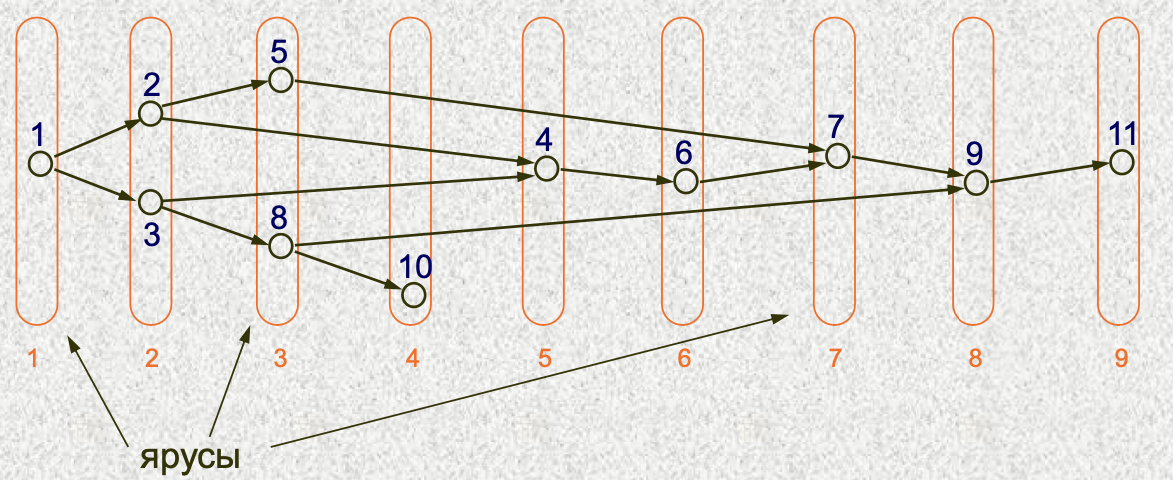
\includegraphics[width=0.2\textwidth]{pics/layered-graph-algo.png}
\end{center}

% -------- source --------
\bigbreak
[\cite{super_computers_lections} 134-137, 709-714]

\vfill\null
\columnbreak
%---------------------
\end{multicols}
\end{tcolorbox}
% --- END OF PAGE ----



% --- BEGIN OF PAGE ----
\newpage
\begin{tcolorbox}[colback=white, left=0mm, right=0mm]
\begin{multicols}{4}
%---------------------0--------------------

\vfill\null
\columnbreak
%---------------------1--------------------
\textbf{\LARGE dop 30. Виды параллельной обработки данных. Компьютеры с общей и распределенной памятью. Производительность вычислительных систем, методы оценки и измерения.}\\

Виды параллельной обработки данных:
\begin{itemize}
    \item Параллельная обработка
    \item Конвейерная обработка
\end{itemize}

При параллельной обработке несколько независимых устройств выполняют какую-то задачу (увеличение производительности достигается за счет количества независимо работающих устройств).\\
При конвейерной обработке процесс разбивается на некоторые этапы, которые выполняются последовательно. Выйгрыш в производительности достигается за счет совмещения операций, которые ранее могли быть разнесены во времени. Для конвейерной обрабоки существует некоторая задержка для того, чтобы заполнить все этапы, но после заполнения всех этапов происходит ускорение обработки. $T = L + (N - 1)$, где $T$ - общее время обработки, $L$ - число ступеней конвейера, $N$ - размер входных данных.\\

\begin{wrapfigure}{r}{0.1\textwidth}
    \centering
    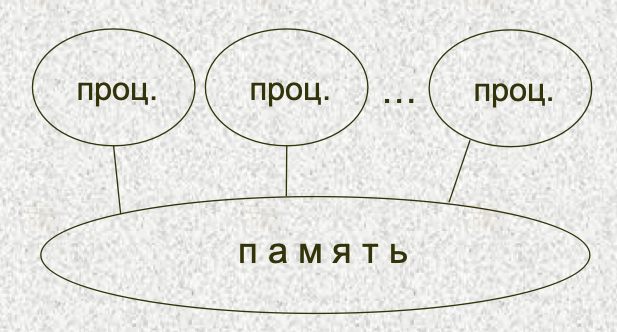
\includegraphics[width=0.1\textwidth]{pics/smp-computer.png}
\end{wrapfigure}

Компьютеры с общей памятью (SMP - Shared Memory Processors / Symmetric MultiProcessor), в SMP-компьютерах все, кроме процессоров, в одном экземпляре: образ ОС, память, подсистема ввода-вывода.\\
Плюс - относительная простота параллельного программирования
Минус - сложность увеличения числа процессоров (роста производительности)\\


\begin{wrapfigure}{r}{0.1\textwidth}
    \centering
    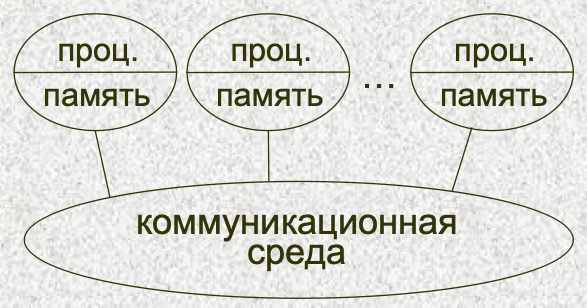
\includegraphics[width=0.1\textwidth]{pics/distributed-memory-computer.png}
\end{wrapfigure}

Компьютеры с распределенной памятью состоят из вычислительных узлов, каждый из которых является полноценным компьютером со своей памятью, ОС, устройствами ввода-вывода и т.п., взаимодействующих друг с другом через коммуникационную среду.\\
Плюс - относительная простота увеличения числа процессоров (роста производительности)\\
Минус - сложность параллельного программирования.\\

Основные показатели эффективности:\\
\begin{itemize}
    \item $p$ - число процессоров
    \item $T_{1}$ - время работы программы на одном процессоре
    \item $T_{p}$ - время работы программы на $p$ процессорах
    \item $S = T_{1} / T_{p}$ - ускорение (speedup) выполнения распараллеленной программы на $p$ процессорах (если $S = p$ - линейное ускорение, если $S > p$ - суперлинейное ускорение)
    \item Эффективность реализации - $R_{max} / R_{peak}$ - отношение реальной производительности к пиковой производительности (тк пиковая производительность на практике недостижима, то эффективность реализации всегда меньше 1)
    \item Эффективность распараллеливания $E = S / p$ - определяет среднюю долю времени выполнения параллельного алгоритма, в течение которого процессоры реально используются для решения задачи
    \item Стоимость вычислений - $C = pT_{p}$
    \item $T_{0} = pT_{p} - T_{1}$ - суммарные накладные расходы
    \item Масштабируемость (scalability) - способность системы увеличивать свою производительность при добавлении ресурсов. Вертикальная масштабируемость - замена платформы, в которой функционирует система на новую, с большей производительностью. Горизонтальная масштабируемость - увеличение производительности за счет добавления дополнительных программных или аппаратных средств
    \item $W$ - вычислительная сложность задачи (кол-во основных вычислительных шагов лучшего последовательного алгоритма, необходимого для решения задачи на одном процессоре)
    \item Сильная масштабируемость - зависимость производительности $R$ от количества процессоров при фиксированной вычислительной сложности ($W = const$)
    \item Масштабируемость вширь (wide scaling) - зависимость производительности $R$ от вычислительной сложности задачи $W$ при фиксированном числе процессоров ($p = const)$
    \item Слабая масштабируемость (weak scaling) — зависимость производительности $R$ от количества процессоров $p$ при фиксированной вычислительной сложности задачи в пересчёте на один процессор ($W/p = const$).
\end{itemize}

% -------- source --------
\bigbreak
[\cite{super_computers_lections} слайды 121-128, 191-193, 158-183]

\vfill\null
\columnbreak
%---------------------2--------------------
%\input{tickets/t_dop28}
\vfill\null
\columnbreak
%---------------------3--------------------
\textbf{\LARGE dop 26. Основные понятия теоpии pазностных схем: аппpоксимация, устойчивость, сходимость.}

Пусть дана исходная дифференциальная задача, которую мы запишем в виде
\begin{equation*}
    Lu(x)=f(x), \eqno(1)
\end{equation*}
где $x \in G$ , $G$ — область m-мерного пространства, $f(x)$ — заданная
функция, $L$ — линейный дифференциальный оператор. Предполагается, что дополнительные условия (типа начальных и граничных
условий) учтены оператором $L$ и правой частью $f$.

Для построения разностной схемы вводится сетка
$G_h$ — конечное множество точек, принадлежащих $G$, плотность распределения которых характеризуется параметром $h$ — шагом сетки.

В общем случае параметр $h$ — вектор, причем определена $|h|$ — длина вектора $h$. Обычно сетка $G_h$ выбирается так, что при
$|h| \rightarrow0$ множество $G_h$ стремится заполнить всю область $G$. Функция, определенная в точках сетки $G$, называется сеточной функцией.

После введения сетки $G_h$ следует заменить в уравнении (1) дифференциальный оператор $L$ разностным оператором $L_h$, правую
часть $f(x)$ — сеточной функцией $\varphi_n(x)$. В результате получим систему разностных уравнений
\begin{equation*}
    L_hy_h(x)=\varphi_h(x), \; x\in G_h, \eqno(2)
\end{equation*}
которая называется разностной схемой или разностной задачей.
% В отличие от дифференциального уравнения решение разностной
% задачи будем обозначать буквой $y$.

Заметим, что свойство аппроксимации означает близость разностного оператора к дифференциальному. Отсюда еще не следует, вообще говоря, близость
решений дифференциального и разностного уравнений. Свойство устойчивости разностной схемы является ее внутренним свойством, не зависящим от того, аппроксимирует ли эта схема какое-либо
дифференциальное уравнение. Оказывается, однако, что
если разностная схема аппроксимирует корректно поставленную задачу и устойчива, то ее решение сходится при $|h|\rightarrow 0$ к решению исходной дифференциальной задачи.

Будем считать, что решение $u(x)$ задачи (1) принадлежит линейному нормированному пространству $B_0, ||\cdot||_0$ —норма в $B_0$. Например, $B_0=C[a,b]$, $||u||_0 = \max_{x\in[a,b]} |u(x)|$. Аналогично считаем, что сеточные функции $y_h(x), \varphi_h(x)$ являются элементами линейного
нормированного пространства (пространства сеточных функций) $B_h$ с нормой $||\cdot||_h$. По существу, имеем семейство линейных нормированных пространств, зависящее от параметра h.

Чтобы иметь возможность сравнивать функции из различных пространств, вводится оператор проектирования $p_h: B_0 \rightarrow B_h$. Это,
по определению, линейный оператор, сопоставляющий каждой функции из $B_0$ некоторую функцию из $B_h$. Для функции $u\in B_0$ обозначим через $u_h$ ее проекцию на пространство $B_h$ т. е. $u_h(x) = p_h u(x)$.

В дальнейшем будем требовать, чтобы нормы в $B_h$ были согласованы с нормой в исходном пространстве $B_0$. Это означает, что для любой $u \in B_0$ выполняется условие
\begin{equation*}
    \lim_{|h| \rightarrow 0}||p_h u||_h=||u||_0 \eqno(3)
\end{equation*}

Требование согласования норм обеспечивает единственность предела сеточных функций при $|h|\rightarrow0$.

Пусть $u(x)$ — решение исходной задачи (1) и $y_h(x)$ — решение разностной задачи (2).

\textbf{Определение 1.} Сеточная функция $z_h(x) = y_h(x) - p_h u(x), x\in G_h$, называется \textit{погрешностью разностной схемы} (2).

Подставим $y_h(x) = p_hu(x) + z_h(x)$ в уравнение (2). Тогда получим, что погрешность $z_h(x)$ удовлетворяет уравнению
\begin{equation*}
    L_h z_h(x) = \psi_h(x), x\in G_h \eqno(4)
\end{equation*}
где
\begin{equation*}
    \psi_h(x) = \varphi_h(x) - L_h(p_h u(x))\equiv \varphi_h(x) - L_h u_h(x) \eqno(5)
\end{equation*}

\textbf{Определение 2.} Сеточная функция $\psi_h(x)$, определенная
формулой (5), называется \textit{погрешностью аппроксимации разностной задачи} (2) на решении исходной дифференциальной задачи (1).

Преобразуем выражение для $\psi_h(х)$. Проектируя уравнение (1) на сетку $G_h$, получим
\begin{equation}\nonumber
p_h Lu(x)=p_h f(x)
\end{equation}
или, учитывая принятые обозначения,
\begin{equation*}
(Lu)_h(x)=f_h(x) \eqno(6)
\end{equation*}
Из (5) и (6) получаем
\begin{equation}\nonumber
\psi_h(x)=\big[(Lu)_h(x)-L_hu_h(x)\big]+(\varphi_h(x)-f_h(x))
\end{equation}
т.е.
\begin{equation}\nonumber
\psi_h(x)=\psi_{h,1}(x) + \psi_{h,2}(x)
\end{equation}
где
\begin{equation*}
    \psi_{h,1}(x) = (Lu)_h(x)-L_hu_h(x), \psi_{h,2}(x) = \varphi_h(x)-f_h(x) \eqno(7)
\end{equation*}
\textbf{Определение 3.} Функции $\psi_{h,1}(x)$ и $\psi_{h,2}(x)$ называются, соответственно, погрешностью аппроксимации дифференциального
оператора $L$ разностным оператором $L_h$ и погрешностью аппроксимации правой части.

\textbf{Определение 4.} Говорят, что разностная задача (2) аппроксимирует исходную задачу (1), если $||\psi_h||_h \rightarrow 0$ при $|h|\rightarrow0$. Разностная схема имеет $k$-й порядок аппроксимации, если существуют
постоянные $k>0, M_1>0$, не зависящие от $h$ и такие, что
\begin{equation}\nonumber
||\psi_h||_h \leq M_1|h|^k.
\end{equation}
Аналогично определяются погрешность аппроксимации и порядок погрешности аппроксимации правых частей и дифференциального оператора.

\textbf{Определение 5.} Разностная схема (2) называется корректной, если

1) ее решение существует и единственно при любых правых частях $\varphi_h \in B_h$

2) существует постоянная $М_2>0$, не зависящая от $h$ и такая, что при любых $\varphi_h \in B_h$ справедлива оценка
\begin{equation*}
    ||y||_h \leq M_2||\varphi_h||_h \eqno(8)
\end{equation*}

Свойство 2), означающее непрерывную зависимость, равномерную относительно $h$, решения разностной задачи от правой части, называется \textit{устойчивостью} разностной схемы. Заметим, что требование 1) эквивалентно существованию оператора $L_h^{-1}$, обратного оператору $L_h$, а требование 2) эквивалентно равномерной по $h$
ограниченности оператора $L_h^{-1}$.

\textbf{Определение 6.} Решение разностной задачи (2) сходится к решению дифференциальной задачи (1), если при $|h|\rightarrow0$
\begin{equation}\nonumber
||y_h - p_hu||_h \rightarrow 0.
\end{equation}

Разностная схема имеет $k$-й порядок точности, если существуют постоянные $k>0, M_3>0$, не зависящие от $h$ и такие, что
\begin{equation}\nonumber
||y_h-\rho_hu||_h \leq M_3|h|^k.
\end{equation}

\textbf{Теорема.} Пусть дифференциальная задача (1) поставлена корректно,
разностная схема (2) является корректной и аппроксимирует исходную задачу (1). Тогда решение разностной задачи (2) сходится
к решению исходной задачи (1), причем порядок точности совпадает с порядком аппроксимации.

\textbf{Доказательство.} Доказательство следует прямо из определений. Действительно, уравнение для погрешности (4) имеет ту же структуру, что
и разностная задача (2). Поэтому из требования корректности следует оценка
\begin{equation*}
    ||z_h||_h \leq M_2||\psi_h||_h \eqno(9)
\end{equation*}
Поскольку константа $M_2$ не зависит от $h$, получаем, что при $||\psi_h||_h \rightarrow 0$
норма погрешности $z_h$ также стремится к нулю, т. е. схема сходится. Если $||\psi_h||_h \leq M_1|h|^k$, то из (9) получим
\begin{equation}\nonumber
||z_h||_h \leq M_1M_2|h|^k
\end{equation}
т. е. разностная схема имеет k-й порядок точности. $\blacksquare$

Значение приведенной выше теоремы состоит в том, что онапозволяет разделить изучение сходимости на два отдельных этапа: доказательство аппроксимации и доказательство устойчивости.
Обычно более сложным этапом является исследование устойчивости, которое состоит в получении оценок вида (8), называемых
априорными оценками.





% -------- source --------
\bigbreak
% [\cite[9.2 - 9.3]{dragonbook}]
\href{http://samarskii.ru/books/book1989.pdf}{Самарский А.А., Гулин А.В. Численные методы, 286 страница}
\vfill\null
\columnbreak
%---------------------
\end{multicols}
\end{tcolorbox}
% --- END OF PAGE ----


% --- BEGIN OF REFERENCES PAGE ----
\newpage
\printbibliography
% --- END OF REFERENCES PAGE ---


\end{document}